\documentclass[twoside, english, notitlepage, 11pt]{uiofysmaster}

\usepackage{packages}

\allowdisplaybreaks

\addbibresource{references.bib}

\author{Sebastian Gregorius Winther-Larsen}
\title{\textbf{AQUADUCT} \\ 
    \textbf{A}b Initio \textbf{Qua}ntum 
    \textbf{D}ynamics \\ \textbf{U}sing 
    \textbf{C}oupled Cluster in 
    \textbf{T}ime
}
\date{\today}

\begin{document}

\frontmatter
    \maketitle

    \begin{abstract}
    We advance the Coupled Cluster method's foray into the time-dependent realm, 
by implementing a robust solver based on the orbital-adaptive time-dependent 
Coupled Cluster (OATDCC)\cite{kvaal2012ab} method.
This involves implementing both a simplified static
orbital time-dependent coupled cluster solver with single and double excitations 
(TDCCSD) and an orbital-adaptive scheme with double excitations (OATDCCD).
To supplement the time-dependent methods we implement several ground state 
solvers based on the Lagrangian Coupled Cluster formulation, with single and double 
excitations, as well as a non-orthogonal orbital-optimised Coupled Cluster (NOCC)
solver\cite{myhre2018demonstrating}.

We construct several quantum dot basis sets with different potential functions
in one- and two dimensions, including interactions with magnetic fields.
What is more, we also implemet an 
interface with popular quantum chemistry software modules PySCF\cite{PYSCF}
and Psi4\cite{parrish2017psi4} for extraction of additional 
basis sets for atoms and molecules. The quantum systems are allowed to vary with time 
by addition of a time-dependent addition to the Hamiltonian, with which we simulate 
a laser field in the dipole approximation.

As a validation we reproduce results from the scientific literature, both for 
atoms, molecules and quantum dots. We show that our methods leads to convergence in 
the ever-increasing basis set size limit, for simple quantum dot systems. For the 
same quantum dot system, we show the sensitivity of the system to the frequency of 
a driving oscillating field. Frequencies closer to the resonant frequency 
leads to exctiations and increased energy. We are able to simulate systems that 
are fairly large - quantum dots in one- and two dimensions with up to twelve 
electrons. For systems that meander far from the reference state, we show that 
the orbital-adaptive method has far superior stability, compared with the 
method with static orbitals.

For all quantum dot system we find 
strong comformity with the harmonic potential theorem\cite{kohn1961cyclotron},
yet we see slight many-body 
effect for a two-dimensional double dot system. The two-dimensional quantum dots 
influenced by a homogoenous, static magnetic field in the form of an angular 
momentum operator, result in a split in the dipole spectrum of the system. This
is also in accordance with the harmonic potential theorem.
The difference between the two frequencies in the new spectrum is the same as the
Larmor frequency of the magnetic field, within acceptable tolerance levels. 
    \end{abstract}
    
    \begin{acknowledgements}
    As a project such as this eventually comes to an end, for better or for
worse\footnote{I have always believed that even an existence with severe stress is preferred
compared to an existence without purpose.},
the custom is to devote some words in a message of gratitude. After all, 
there are people in one's life that make everything a bit more enjoyable through their
support - be it scientific or spiritual.

Firstly, I would like to thank my supervisor Morten. You welcomed me, willingly, with open arms,
and despite of my previous background in finance, into the computational physics group. I value your 
unterminable optimism - after a chat with you I always feel invigorated and motivated. You bring 
great inspiration to your students and others around you.

Words of emphatic thanks are also imparted in the direction of my serendipitous co-supervisor Håkon.
Your aid and insights have proven invaluable beyond a doubt. I consider myself very lucky to have
someone examine my 
work as closely as you have done. More than that, I am delighted to have a friend like you.

To my partner in despair, Øyvind, who has been invaluable in all respects. You have that one personal 
trait that I look up to with high regard: unbounded resolve and grit that makes for true
strength of character. I have found it motivating to work beside you and I am thankful for your 
friendship over the the many months (years!) we have struggled with very difficult physics together.

I would like to give my regards to the amazing people that make up the computational physics graduate
students.
If nothing more, you definitely make for the most enjoyable luncheons that oft-times include
pristine
philosphical discussions. The tales of the camaraderie of this gang of nonconformists will 
undoubtedly become material for an operette or at least some form of low-budget musical theatre.

I am also thankful to the two troupes of troubadours I have been affiliated with during my time as a student 
at the University of Oslo. It was in the ranks\footnote{I am not sure if ``rank'' is the best word, because 
if Biørneblæs were even able to line up, it would more closely resemble a pile of overcooked spaghetti
than ranks and files.} of Studentorchestert Biørneblæs where I first 
picked up the saxophone, and here I found tremendous musical joy. Eventually I was head-hunted to 
become Il Maestro of Blindern Haarn oc Blaese. An event that actually \emph{was}
the basis of some form of very low-budget musical theatre. One should never let the (low) quality
of the music be hindrance to a great orchestral experience.

To Vilde: I feel fortunate to have someone like you as my companion. The adventures we've had make up
some of my most treasured memories, and I hope we will have many more together. Thank you for your 
patience, love and encouragement throughout these extra-ordinary months.

\paragraph{Collaboration details}

The software that has been developed as part of this thesis was developed in joint 
effort between \citeauthor{islandwind2019}\cite{islandwind2019} and myself. As such,
it exists as only one product, as we saw fit to join forces instead of manufacturing two 
duplicates of the same invention.
    \end{acknowledgements} 

    %\setcounter{tocdepth}{1}
    \tableofcontents
    %\listoffigures

\mainmatter

    \chapter{Introduction}

    The aim and raison d'étre of this thesis is to implement methods that enables the 
    study of many-body quantum systems in time. The word `ìmplement'' entails construction 
    of numerical solvers on a computer. Such computational modelling have since its 
    inception around the middle of the last century become present in all of the natural 
    sciences, and have since made its foray in the social sciences as well. In the 
    natural sciences, one could argue that computation plays as big a role as the two 
    conventional congregations of theory and experiment. In physics, computations are 
    a central component in a vast area of fields so diverse as
    quantum chromodynamics\cite{pederiva2018computing,vege2019solving},
    molecular dynamics\cite{stende2017constructing,treider2017speeding} and 
    astrophysics\cite{sand2016massive}.

    Quantum mechanics is the description of the behaviour of matter and light in all 
    its details, and in particular of the happenings on an atomic scale. A state of 
    a quantum system is described by a wavefunction $\Psi(\vb{r}, t)$, which provides 
    us with all there is to know about a particular system. We can determine
    $\Psi(\vb{r}, t)$
    at any point in the future by solving the Schrödinger equation, given the inital 
    state of the system $\Psi(\vb{r}, t_0)$,
    \begin{equation}
        i\hbar \frac{\partial}{\partial t} \Psi(\vb{r}, t) = \hat{H} \Psi(\vb{r}, t).
    \end{equation}
    Our ability to solve the Schrödinger equation analytically is constrained to only 
    a few quantum systems, and vanishes rapidly as the number of constituent particles in 
    such a system exceed just a few. It has therefore been necessary to extend the chalk and 
    the blackboard with numerics and a computer. The underlying theory for all of chemistry 
    is well-known and has been known for more than half a century, but the only element 
    we are able to solve on the blackboard is the the very simplest element, hydrogen.
    Adding an electron to the quantum hydrogren atom results in an analytically 
    unsolvable Schrödinger equation. As such, in order to \emph{solve chemistry} we 
    need numerical approximations.


\section{The Quantum Many-Body Problem}

    We have established that solving the Schrödinger equations exactly by hand is 
    impossible in the overwhelming majority of interesting cases. For this reason, 
    a plethora of computational, approximative methods have been developed aiming 
    to solve the many-body Schrödinger equation. Starting from first principles,
    or \emph{ab initio}, the goal of such algorithms is to procure some information
    about a quantum system in a reasonable amount of time. In order to accomplish 
    this, some sacrifices must be made in the form of simplifications. 

    The Hartree-Fock
    method\cite{hartree1928wave,fock1930naherungsmethode,szabo2012modern} which 
    has seen extensive use since its inception in 1930
    employs a mean-field appriximation, which provides an efficiently computed result, 
    but it is not very accurate. The most popular approximative method is without doubt 
    the density functional theory (DFT), developed by Kohn and Sham in
    1965\cite{kohn1965self}, which simplifies the quantum many-body problem by reformulating 
    it in terms of eletron number density. However, DFT is also insufficient if one requires a 
    high degree of accuracy.

    It is possible to solve a quantum many-body problem  ``correctly'' by direct diagonalisation 
    of the Hamiltionian, often called Full Configuration Interaction (FCI). Such a method 
    will yield an absolutely accurate result in the limit of an infinite orbital basis set,
    but it suffers from exponential complexity scaling\cite{helgaker2014molecular}.
    A sophisticated Monte-Carlo scheme, like Diffusion Monte-Carlo (DMC) can in principle 
    provide the exact solution to the Schrödinger equation by imaginary time-evolution 
    of an inital wave function ansatz\cite{hammond1994monte}. The high dependence of the 
    initial guess is problematic. What is more, the method often require the input of
    another less accurate method as a starting point. Another 
    example of a similar method is the Variational Monte-Carlo (VMC) method, which is
    simpler and faster than DMC, but not as accurate.

    Since the Hartree-Fock method is the earliest of methods designed to solve the quantum 
    many-body problem, it has become the purpose of all other many-body methods to describe 
    \emph{electron correlation}, defined as representing the difference between the 
    Hartree-Fock description of the electronic wavefunction and the exact solution of 
    the Schrödinger eqution. The simplest approach to treat the electron correlation
    is by performing a Configurations Interaction (CI) expansion,
    \begin{equation}
        \Psi = \Phi_\text{HF} 
            + \sum_{ia} C^i_a\Phi^a_i 
            + \sum_{\substack{i < j \\ a < b}} C^{ij}_{ab} \Phi^{ab}_{ij} + \dots,
    \end{equation}
    where $\Phi^a_i$ is a \emph{singly excited} configuration. We obtain the exact,
    Full Configuration Interaction, by including all terms in the CI expansion.
    Truncating the configurations interactions at a decided excitation may at first 
    seem like a good idea. It is common to perform such a truncation after the 
    double-excitation level, producing Configuration Interaction Singles Doubles (CISD).

    Two important properties that a many-body method must incorporate is \emph{size-extensivity}
    and \emph{size-consistency}. A quantum-mechanical model is said to be \emph{extensive}
    if the energy of the system computed with this model scales with the size of the 
    system\cite{bartlett1978many}. For systems of non-interacting helium atoms, for instance,
    we must have that $E(N\text{He}) = NE(\text{He})$. Moreover, a model is \emph{size-consistent}
    if the energies of two systems $A$ and $B$ and of the combined system $AB$, with 
    $A$ and $B$ very far apart, computed in equivalent ways, satify
    $E(AB) = E(A) + E(B)$\cite{pople1976theoretical}. It can be shown that 
    truncated CI does \emph{not} comply with the concept of
    extensivity\cite{shavitt2009many}.

    A class of methods of which most constituents provide proper \emph{extensive} model
    descriptions is Many Body Perturbation Theory (MBPT)\cite{brueckner1955approximate}.
    MBPT can also be truncated at a certain 
    excitation level, in the same manner as truncated Configuration Interaction. 
    The linked-diagram theorem\cite{goldstone1957derivation}, states that a 
    particular perturbation expansion can be expressed by ``linked terms''
    only\footnote{A thorough treatment of these terms are found in the end of
    \autoref{ch:perturbation}},
    leading to the Coupled Cluster method\cite{coester1958bound,coester1960short}.
    Coupled Cluster has become one of the most prevalent methods in quantum chemistry,
    as it is very accurate, whilst maintaining size-consistency and -extensivity.
    The Coupled Cluster method also has elegant truncation levels, similar to the 
    truncated Configuration Interaction method\footnote{Coupled Cluster and
    Configuration Interaction has an elegant correspondence,
    see \autoref{app:cc_vs_ci}}.

    Computational scaling of \emph{ab initio} quantum mechanical models range from 
    $\mathcal{O}(N!)$ for Full Configuration Interaction (FCI), via $\mathcal{O}(N^6)$ 
    for Coupled Cluster Singled Doubles with Perturbed Triples (CCSD(T)) to 
    $\mathcal{O}(N^4)$ for formal Hartree-Fock (HF)\cite{ratcliff2017challenges}.


\section{Goals}

    The specific task of this thesis is to study the time evolution of quantum 
    mechanical systems using the Coupled Cluster method. In particular this 
    pertains to the study of the time-dependent electronic systems, with an emphasis 
    on quantum dots. By use of proper object-orientation the implementation should 
    also be used to study simple atoms and molecules in three dimensions.
    The aim should be to 
    extend the formalism and algorithms developed in the thesis of 
    \citeauthor{haakon2017time}\cite{haakon2017time}.

    The these progression milestones have been split into the following steps,

    \begin{enumerate}
        \item Write a Coupled Cluster Doubles code with double exciations (CCD)
            capable of solving a system of two electrons in two or three dimensions 
            in a single harmonic oscillator well.
        \item Extend Coupled Cluster solver to include singles excitations (CCSD)
            and time evolution with static orbitals (TDCCSD). Moreover, expand system
            implementations to include more interesting systems, for example double
            potential wells or simple atoms.
        \item Include orbital dependencies in the time-dependent coupled cluster solver, as 
            discussed by \citeauthor{kvaal2012ab}\cite{kvaal2012ab}.
    \end{enumerate}

\section{Our Contributions}

    There already exists an abundance of optimised and well-tested ab inito quantum chemistry 
    software packages. As such we have not sought to build software meant to compete 
    with such software, but function as a supplement. As far as we know 
    there is currently no software that allows for time-dependent Coupled Cluster 
    computations in widespread use, making our contribution worthwhile. The interest 
    we have seen for our work at the Hylleraas centre at the University of Oslo 
    is testament to this\cite{islandwind2019numerically}.

    We have constructed two modules in the Python programming language that works
    well in conjunction, but 
    can also be used separately. The module \lstinline{coupled_cluster}, as the  
    name suggests contains all our Coupled Cluster solvers, both ground state and 
    time-dependent. The module \lstinline{quantum_systems} provides basis sets
    designed to work with the \lstinline{coupled_cluster} module. The 
    \lstinline{quantum_systems} module also contains functions for extracting basis sets 
    from the very popular quantum chemistry modules \lstinline{PySCF}\cite{PYSCF}
    and Psi4\cite{parrish2017psi4}. The source code for the \lstinline{coupled_cluster} module 
    can be found at
    \url{github.com/Schoyen/coupled-cluster}\footnote{At the time this document is 
    first printed, the source code may not be public. We plan to make the source code 
    open and public as soon as possible.} and documentation at 
    \url{www.coupledcluster.com}.
    The source code for the \lstinline{quantum_systems} module 
    can be found at
    \url{github.com/Schoyen/quantum-systems} and documentation at 
    \url{Schoyen.github.io/quantum-systems}.

    We have chosen Python as a development language for a couple of reasons. 
    First, even though Python is essently a  ``scripting language'', in the sense 
    that it is usually slower than a compiled language like \CC,
    most of our computations are matrix or tensor computations which are very fast
    in Python. We do matrix multiplications and linear algebra in NumPy, which 
    is very fast because of its use of Basic Liner Algebra Subprograms (BLAS) 
    and Linear Algebra PACKage (LAPACK).
    Both implemented in Fortran, BLAS consists of a low-level matrix and vector 
    arithmetic operations, while LAPACK is a collection of common algorithms 
    used in linear algebra such as routines for solving systems of linear 
    equations. For heavy operations that are not vectorisable, we have found
    just-in-time compilations with numba very beneficial.

    Second, Python is a high level language which has sped up development greatly 
    compared to developing in a lower level language. For this reason we 
    have a feeling that we have accomplished more than we would have 
    otherwise. The drawback of developing in a higher level language is the 
    lack of low level control, like memory management. 

\section{Structure of this Thesis}

    This thesis consists of five main parts. The first part, \emph{Fundamentals} 
    introduces the basis of quantum mechanics as well as the second quantisation 
    formalism.
    
    In the second part, \emph{Quantum Many-Body Approximation}, we 
    thoroughly present three many-body methods, each in its own chapter.
    We start with a chapter on \emph{Hartree-Fock Theory}, because this is 
    the first ab initio many-body method that saw truly widespread use, but 
    also because the Lagrange multiplier path we take to derive the method is 
    similar to what we will do later, when we talk about Lagrangian Coupled Cluster.
    We also introduce a time-dependent Hartree-Fock scheme here.
    Next, we present many-body \emph{Perturbation Theory}, which is often used as
    a supplement to other many-body methods, but it also highlights the origins 
    of the Coupled Cluster method, the topic of the next chapter.
    We derive both Brillouin-Wigner- and Rayleigh-Schrödinger Perturbation theory. 
    In the chapter on \emph{Coupled Cluster} we provide a detailed derivation
    of the Coupled Cluster equations, before detailing the problems caused 
    by the method's non-variational nature. This leads naturally to 
    the Lagrangian formulation of Coupled Cluster\cite{helgaker1988analytical}
    and the bivariational principle\cite{arponen1983variational}. Lastly,
    we introduce time-dependent Coupled Cluster theory, with both static and 
    adaptive orbitals\cite{kvaal2012ab}.

    In \emph{Implementation}, the third part of the thesis, we bestow upon the reader 
    a specification of the two python modules, \lstinline{quantum_systems} 
    and \lstinline{coupled_cluster}. Furthermore, we seek to explain the machinery
    in the two python modules, and their functionality. 

    In the fourth part of the thesis, we provide \emph{Results} generated with the
    coupled cluster solvers we have implemented. We start by a validation against
    some existing literature on time-dependent ab initio solvers. This includes 
    the reproduction of several results from relatively well-known articles. 
    The second and last chapter in this part contains the central results of 
    this thesis. Here we provide results from simulations of one- and two-dimensional 
    quantum dots, as well as two-dimensional quantum 
    dots acted on by an approximation of a magnetic field. Becuase this study 
    has been conducted in close conjunction with
    \citeauthor{islandwind2019}, more results that are computed with the 
    same solvers, relating to atoms and molecules can be found in Ref.
    \cite{islandwind2019}.
   
    Lastly, in the fifth and final section we impart a \emph{Conclusion} and 
    some suggestions for future work in the same field of study.


    \part{Fundamentals}

        \chapter{Quantum Mechanics}
    \epigraph{Hierzu ist es notwendig, die Energy nicht als eine stetige
    unbeschränkt teilbare, sondern als eine discrete, ause einer ganzen
    Zahl von endlichen gleichen Teilen zusammengesetzte Grösse 
    aufzufassen.}
    {--- Max Planck}


\section{Classical Mechanics}

    The formalism used in quantum mechanics largely stems from William Rowan Hamilton's 
    formulation of classical mechanics. Through the process of canonical
    quantisation any classical model of a physical system is turned into
    a quantum mechanical model.

    In Hamilton's formulation of classical mechanics, a complete description of a system
    of N particles is described by a set of canonical coordinates 
    $q = (\vec{q}_1, \dots, \vec{p}_N)$ and corresponding conjugate momenta
    $p = (\vec{p}_1, \dots \vec{p}_N)$. Together, each pair of coordinate and momentum
    form a point $\xi = (q, p)$ in phase space, which is a space of all possible states
    of the system. Moreover, pairs of generalised coordinates and conjugate
    momenta are canonical if they satisfy the Poisson brackets so that 
    $\{q_i, p_k\} = \delta_{ij}$. The Poisson bracket of two functions is defined as 

    \begin{equation}
        \label{eq:poisson_bracket}
        \{f, g\} = \frac{\partial f}{\partial q} \frac{\partial g}{\partial g}
        - \frac{\partial f}{\partial p} \frac{\partial g}{\partial q}.
    \end{equation}

    The governing equations of motion in a classical system is Hamilton's equations,

    \begin{align}
        \dot{q} &= \frac{\partial}{\partial p} \mathscr{H}(q, p) \\
        \dot{p} &= -\frac{\partial}{\partial q} \mathscr{H}(q, p)
    \end{align}

    where $\mathscr{H}(q, p)$ is the Hamiltonian, a function for the total energy of the
    system. Hamilton's equations may also be stated in terms of the Poisson brackets,

    \begin{equation}
        \frac{dp_i}{dt} = \{p_i, \mathscr{H}\}, \ \frac{dq_i}{dt} = \{q_i, \mathscr{H}\}.
    \end{equation}

    A system consisting of $N$ of equal mass $m$, subject forces caused by an external
    potential, as well as acting on each other with forces stemming from a central
    potetntial $w(q_ij)$ has the following Hamiltonian,

    \begin{equation}
        \mathscr{H}(q, p) = \mathscr{T}(q) + \mathscr{V}(p) + \mathscr{W}(p) 
            = \frac{1}{2m}\sum_{i} \abs{\vec{p}_i}^2 + \sum_{i} v(\vec{r}_i)
                + \frac{1}{2}\sum_{i<j} w(\vec{r_{ij}}).
    \end{equation}

    This Hamiltonian conveniently contains several parts - the kinetic energy, the
    external potential energy and the interaction energy; denoted by $\mathscr{T}$,
    $\mathscr{V}$ and $\mathscr{W}$ respectively.

\section{Canonical Quantisation}

    In order to transition from a classical system to a quantum system, we move from 
    the classucal phase space to the Hilbert space, through the procedure known as 
    canonical, or first\footnote{Second quantisation comes later.}-, quantisation.
    Whilst the state of a classical system is a point in phase space, a quantum state
    is a complex-valued state vector in discrete, infinite-dimensional, Hilbert space,
    that is a complete vector space equipped with an inner product. This space
    is most commonly chosen to be the space of square-integrable functions $\Psi$,
    dependent on all coordinates
    
    \begin{equation}
        \Psi = \Psi(x_1, x_2, \dots, x_N).
    \end{equation}
    
    These functions
    are dubbed wavefunctions and are maps from a point $(x_1, \dots, x_N)$ in
    configuration space to the complex vector space,

    \begin{equation}
        \Psi: X^N \to \mathds{C}.
    \end{equation}

    It has been widely discussed how such an object can represent the state of a 
    particle. The answer is provided by Max Born's probabilistic interpretation,
    which says that $\abs{\Psi(x_1, \dots, x_N)}^2$, gives the probability of finding
    the particle at a certain position. For a situation with one particle in one
    dimension we have,

    \begin{equation}
        \int_a^b \abs{\Psi(x)}^2 dx = 
        \left\{\begin{aligned}
            \text{probability of finding the} \\
            \text{particle between $a$ and $b$}
        \end{aligned}\right\}
    \end{equation}

    while $\abs{\Psi(x_1, x_2, \dots, x_N)}^2$ is the probability density for locating
    all particles at the point $(x_1, \dots x_N) \in X^N$. Since the total probability
    must be 1, we are provided with a normalisation condition for the wavefunction,
    
    \begin{equation}
        \int_{X^N} \abs{\Psi(x_1, x_2, \dots, x_N)}^2 dx_1 dx_2\dots dx_N = \mathds{1}.
    \end{equation}

    The relation between a classical- and quantum decsription of a mechanical system 
    is most clearly seen when the two descriptions are expressed in terms of the same 
    variables. In fact, we may apply \emph{quantisation} of the classical variables to 
    produce the quantum equivalent of the system. The classical phase space variables 
    are changed into quantum observables,
    \begin{equation}
        q_i \to \hat{q}_i, \ p_i \to \hat{p}_i.
    \end{equation}
    The quantum observables are required to satisfy the Heisenberg commutation relation,
    \begin{equation}
        [\hat{q}_i, \hat{p}_j] = i \hbar \delta_{ij},
    \end{equation}
    instead of the Poisson bracket (\autoref{eq:poisson_bracket}). Here $\hbar$ is the 
    reduced Planck's constant. For any general variables $A$ and $B$, this 
    transition can be expressed by subsition between Poission brackets for the 
    classical variables and commutators for the quantum observables,
    \begin{equation}
        \{A, B\} \to \frac{1}{i\hbar}[\hat{A},\hat{B}].
    \end{equation}

    This correspondence between the classical and quantum dynamical equations is 
    directly related to \emph{Ehrenfest's therom}, which states that the classical 
    dynamical equations keep their validity also in the quantum theory, with the 
    classical variables repaced by their corresponding quantum expectation
    values\cite{ehrenfest1927bemerkung}.

\subsection{The Dirac-von Neumann Postulates}

    The following postulates, or axioms, provide a precise and concise description 
    of quantum mechanics in terms of operators on the Hilbert space. There are
    many variations of these postulates, introduced both by their namesakes 
    Paul Adriene Maurice Dirac\cite{dirac1930principles} and John von 
    Neumann\cite{vonNeumann1932foundations}.

    \subsubsection{Hilbert Space}
    A quantum state of an isolated physical system is described by a vector
    with unit norm in a Hilbert space $\mathcal{H}$, 
    a complex vector space equipped with an inner product. The inner product 
    associates a scalar value, which may be either real or complex, with any pair
    of state vectors.
    
    The inner product can be defined as 
    \begin{equation}
        \braket{\psi_\alpha}{\psi_\beta} = \int \psi_\alpha^*(x) \psi_\beta(x)dx,
    \end{equation}
    where $\psi^*$ is the complex conjugate of $\psi$. Here we have introduced 
    Dirac notation, which is very common when describing quantum states. For each 
    quantum state $\ket{\psi_\alpha}$ there exists a dual state $\bra{\psi_\alpha}$.
    We refers to these two vectors as \emph{bra} and \emph{ket} vectors, respectably.
    Some properties of a Dirac-style inner product read
    \begin{align}
        \braket{\psi_\alpha}{\psi_\beta} =& \braket{\psi_\beta}{\psi_\alpha}^* \\
        \bra{\psi_\alpha}\left(z_1\ket{\psi_\beta} + z_2 \ket{\psi_\beta}\right)
            =& z_1 \braket{\psi_\alpha}{\psi_\beta} + z_2\braket{\psi_\alpha}{\psi_\beta} \\
        \braket{\psi_\alpha} \geq& 0,
    \end{align}
    where $z_n = a_n + ib_n$ is some complex number. Notice that in these properties, a 
    superposition of a state wavefunction in the form of linear combination of two other 
    states have appeared. Such superpositions are generally written
    \begin{equation}
        \label{eq:superposition}
        \ket{\psi_\gamma} = z_1\ket{\psi_\alpha} + z_2\ket{\psi_\beta},
    \end{equation}
    where we have produced a new quantum state from two other states. Any two or more
    states may be superposed to produce a new state. Superposition is of fundamental 
    importance to quantum mechanics, and even though the concept is similar to the 
    classical superposition principle for waves in classical physics, "the superposition 
    that occurs in quantum mechanics is of an essentially different nature from any 
    occuring in the classical theory" according 
    to \citeauthor{dirac1930principles}\cite{dirac1930principles}.

    Proceeding with the description of quantum states, a state function $\psi$ is said 
    to be \emph{normal} if its innerproduct with itself is one, $\braket{\psi}{\psi} = 1$.
    Two different state functions are \emph{orthogonal} if their inner product is zero. 
    We have orthogonal functions if $\braket{\psi_\alpha}{\psi_\beta} = \delta_{\alpha\beta}$,
    where $\delta_{\alpha\beta}$ is the Kronecker delta.


    \subsubsection{Observables}
    Each physical observable of a system is accociated with a \emph{hermitian}
    operator acting on the Hilbert space. The eigenstates of each such
    an operator define a \emph{complete}, \emph{orthonormal} basis set of vectors
    $\mathcal{B}$ for the $d$-dimensional Hilbert space,
    \begin{equation}
        \mathcal{B} = \{\ket{i}\}_{i=1}^d
    \end{equation}
    Completeness of the basis set $\mathcal{B}$ means,
    \begin{equation}
        \sum_{i=1}^d \ket{i}\bra{i} = \mathds{1}.
    \end{equation}

    With $\hat{O}$ an operator, \emph{hermiticity} means,
    \begin{equation}
        \bra{\phi}\hat{O}\psi\rangle = \langle\hat{O}\phi\ket{\psi} \equiv \bra{\phi} \hat{O} \ket{\psi}.
    \end{equation}
    This means that the operator $\hat{O}$ is its own Hermitian conjugate,
    \begin{equation}
        \hat{O}^\dagger = \hat{O}.
    \end{equation}
    Some properties of the Hermitian conjugate reads,
    \begin{align}
       (z\hat{O})^\dagger =& z^*\hat{O}^\dagger \\
       (\hat{O}_1 + \hat{O}_2)^\dagger =& \hat{O}_1^\dagger \hat{O}_2^\dagger \\
       (\hat{O}_1\hat{O_2})^\dagger =& \hat{O}_2^\dagger \hat{O}_1^\dagger.
    \end{align}

    \subsubsection{Measurements}
    Physically measurable values, associated with an observable $\hat{O}$ are defined by the 
    eigenvalues $o_n$ of the observable,
    \begin{equation}
        \hat{O}\ket{n} = o_n\ket{n}.
    \end{equation}
    The probability for finding a particular eigenvalue in the measurement is
    \begin{equation}
        p_n = \abs{\braket{n}{\psi}}^2,
    \end{equation}
    with the system in state $\ket{\psi}$ before the measurement, and $\ket{n}$ as the 
    eigenstate corresponding to the eigenvalue $o_n$.
    If the observable $\hat{O}$ is Hermitian, we can write the operators as a spectral 
    decomposition 
    \begin{equation}
        \hat{O} = \sum_{n=1}^d o_n \dyad{n},
    \end{equation}
    where $d$ is the dimensionality of the Hilbert space.

    \subsubsection{Time Evolution}
    In the \emph{Schrödinger picture}
    time evolution of the state vector, $\ket{\psi} = \ket{\psi (t)}$, is given by the Schrödinger
    equation\footnote{In the Schrödinger picture.}.
    \begin{equation}
        i\hbar \frac{d}{dt} \ket{\psi (t)} = \hat{H} \ket{\psi (t)}.
    \end{equation}
    Note that any superposed state, as described by \ref{eq:superposition}, will also be 
    a solution to the Schrödinger equation due to its linearity.

    The Schrödinger equation is first order in the time derivate, meaning that the time 
    evolution $\ket{\psi} = \ket{\psi(t)}$ is uniquely determined by some initial 
    condition $\ket{\psi_0} = \ket{\psi(t_0)}$. $\hat{H}$ is the Hamiltonian of the system,
    which is a \emph{linear}, \emph{hermitian} operator. The Hamiltonian gives rise to the 
    time evolution, which is a \emph{unitary} mapping between quantum states in time,
    \begin{equation}
        \ket{\psi(t)} =  \hat{\mathcal{U}}(t, t_0) \ket{t_0}.
    \end{equation}
    The time evolution operator $\hat{\mathcal{U}}$ is determined by the Hamiltonian 
    through the equaton 
    \begin{equation}
        i\hbar \frac{\partial}{\partial t} \hat{\mathcal{U}}(t, t_0)
            = \hat{H}\hat{\mathcal{U}}(t, t_0),
    \end{equation}
    which follows from the Schrödinger equation. For a time-independent 
    Hamiltonian it is given by 
    \begin{equation}
        \hat{\mathcal{U}}(t, t_0) = e^{-i \hat{H}(t - t_0/\hbar)}.
    \end{equation}
    We see that this time-propagater is Hermitian 
    \begin{equation}
        \hat{\mathcal{U}}\hat{\mathcal{U}}^\dagger 
        = \hat{\mathcal{U}}^\dagger \hat{\mathcal{U}} = 1.
    \end{equation}
    If however $\hat{H}$ is time-dependent, so that the operator at different times do 
    not commute, we may use a mroe general integral expression for the time-propagator,
    \begin{equation}
        \hat{\mathcal{U}}(t, t_0)
         = \sum_{n=0}^\infty (-\frac{i}{\hbar})^n
            \int_{t_0}^t \int_{t_0}^{t_1}dt_1 \int_{t_0}^{t_1}dt_2 \dots \int_{t_0}^{t_{n-1}}
                dt_n \hat{H}(t_1)\hat{H}(t_2) \dots \hat{H}(t_n).
    \end{equation}

    A unitary transformation of states and observables
    \begin{equation}
        \ket{\psi} \to \ket{\psi'} = \hat{U}\ket{\psi}, \ 
        \hat{O} \to \hat{O}' = \hat{U}\hat{O}\hat{U}^\dagger, \ 
        \hat{U}^\dagger\hat{U} = 1.
    \end{equation}
    leads to a different, but equivalent representation of a quantum system.
    The transition to the \emph{Heisenberg picture} is defined by a special
    time-dependent unitary transformation,
    \begin{equation}
        \hat{U} = \hat{\mathcal{U}}^\dagger(t, t_0),
    \end{equation}
    which is the inverse of the time-evolution operator. When applied to the 
    time-dependent state vector of the Schrödinger picture it will cancel 
    the time-dependence
    \begin{equation}
        \ket{\psi}_\text{H} 
        = \hat{\mathcal{U}}^\dagger(t, t_0) \ket{\psi(t)}_\text{S}. 
        = \ket{\psi(t_0)}_\text{S}
    \end{equation}
    The time-dependece is now carried by the observables, rather than the state 
    vectors,
    \begin{equation}
        \hat{O}_\text{H} 
        = \hat{\mathcal{U}}^\dagger(t, t_0)
        \hat{O}_\text{S}
        \hat{\mathcal{U}}(t, t_0),
    \end{equation}
    and the Schrödinger equation is replaced by the Heisenberg equation
    \begin{equation}
        \frac{d}{dt} 
        = \frac{i}{\hbar}[\hat{H}, \hat{O}_\text{H}]
        + \frac{\partial}{\partial t} \hat{O}_\text{H}.
    \end{equation}

    There is a third representation called the \emph{interaction picture}, but we will 
    remain firmly rooted in the Schrödinger picture and halt this general introduction 
    to time-development here. 

\section{The Quantum Hamiltonian}

    The full Hamiltionian for a quantum many-body system can be a large 
    and unwieldy thing. In this study we will constrain ourselves to the study of
    electronic systems. Purely on a phenomenological basis, one would include nuclear
    terms in the Hamiltonian as well. In this study however, we will stay within the
    Born-Oppenheimer approximation and treat the nuclei as stationary particles, thereby
    refraining from introducing terms that involve the motion of nuclei.

    The full  molecular electronic Breit-Pauli Hamiltionian, throrougly described in 
    Helgaker et al.\cite{helgaker2012recent}, contains the following types of terms
    \begin{equation}
        \label{eq:breit_pauli_hamiltonian}
        \hat{H}^{\text{BP}}_{\text{mol}}
        = \begin{cases}
            \hat{H}_{\text{kin}} \quad &\leftarrow \text{kinetic energy} \\
            + \hat{H}_{\text{cou}} \quad &\leftarrow \text{Coulomb interactions} \\
            + \hat{H}_{\text{ee}} \quad &\leftarrow \text{external electric field interaction} \\
            + \hat{H}_Z \quad &\leftarrow \text{Zeeman interactions} \\
            + \hat{H}_{\text{so}} &\leftarrow \text{spin-orbit interactions} \\
            + \hat{H}_{\text{ss}} &\leftarrow \text{spin-spin interactions} \\
            + \hat{H}_{\text{oo}} &\leftarrow \text{orbit-orbit interactions} \\
            + \hat{H}_{\text{dia}} &\leftarrow \alpha^4 \text{ diamagnetic interactions}
        \end{cases}
    \end{equation}
    We will not be working with this giant beast, but will go into some of the most  
    import terms that an electronic Hamiltonian can constitute. 
    
    \paragraph{Kinetic energy}

    The genereal kinetic energy operator is given by
    \begin{equation}
        \label{eq:kinetic_energy_term}
        \hat{H}_{\text{kin}}
            = - \frac{\hbar}{2m}\sum_i \nabla^2_i,
    \end{equation}
    where $\nabla$ is the differential operator and the sum is over all electrons in 
    the system. This term is an example of a one-particle operator as it remains the 
    same for all eletrons and has is contains to terms that would constitute interaction 
    between particles. For a free particle or a gas of non-interacting particles, 
    \autoref{eq:kinetic_energy_term} is sufficient to describe the system. 

    \paragraph{Potential terms}

    By adding a confining potential to the Hamiltonian in addition to the kinetic 
    energy term \autoref{eq:kinetic_energy_term},
    \begin{equation}
        \hat{H} \supset \hat{H}_\text{kin} + \hat{V}
    \end{equation}
    gives rise to much more intersting systems and are the beginning of an approximation 
    of reality. Perhaps the most common is the harmonic oscillator potential, which 
    in one dimension reads 
    \begin{equation}
        \hat{V}(x) = \frac{1}{2}m\omega^2x^2.
    \end{equation}
    This is a very popular confining potential because virtually any oscilaltory motion can 
    be approximated by it, if the amplitude of the oscillations are small. The parabolic 
    potential is the basis of a quantum dot which is a central part of this study. 
    In quantum chemistry we only consider potentials derived from particle-particle 
    interactions, and not such external potentials.

    \paragraph{Coulomb interactions}

    Electrostatic interaction between particles in a molecule or atom is 
    modelled by Coulomb terms in the Hamiltonian. 
    \begin{equation}
            \hat{H}_{\text{cou}} 
                = -\sum_{iK}\frac{k_eZ_Ke^2}{r_{iK}} 
                    + \frac{1}{2}\sum_{i \neq j} \frac{k_e e^2}{r_{ij}} 
                    + \frac{1}{2}\sum_{K \neq L} \frac{k_eZ_K Z_Le^2}{R_{KL}},
    \end{equation}
    where $e$ is the elementary particle charge and $k_e = 1 / 4\pi\epsilon_0$ is the 
    Coulomb constant.
    The first term is the potential between nuclei and electrons, the second term is
    the potential between electrons and the last term is the potential between 
    nuclei. In the Born-Oppenheimer approximaton we ignore the first and third term.

    \paragraph{External electric field interactions}
    
    Applying an electromagnetic field we need to include terms in the Hamiltonian that 
    model the effects of externally applied scalar potential $\phi = \phi(\vb{r}, t)$
    and vector potential $\vb{A} = \vb{A}(\vb{r}, t)$. This will also affect the 
    kinetic energy of the particles, which we therefore include at first,
    \begin{equation}
        \hat{H}_\text{ef} 
            \subset \frac{1}{2m}(\vb{p} + e \vb{A})^2 - e\phi
            = \frac{\hat{\vb{p}}}{2m} + \frac{e}{2m}(\vb{A}\cdot\hat{\vb{p}} + \hat{\vb{p}}\cdot\vb{A})
                + \frac{e^2}{2m}\vb{A}^2 - e\phi.
    \end{equation}
    This Hamiltonian now describes a free partice subject to an external 
    electro field. Since we have already included a term for kinetic energy we 
    now wish to remove it,
    \begin{equation}
        \hat{H}_\text{ef} 
            = - \frac{e}{2m}(\vb{A}\cdot\hat{\vb{p}} + \hat{\vb{p}}\cdot\vb{A})
                + \frac{e^2}{2m}\vb{A}^2 - e\phi.
    \end{equation}

    We assume that the external field has sufficiently large wavelenght compared to the 
    system, making the vector potential uniform in space $\vb{A}(\vb{r}, t) = \vb{A}(t)$
    This approximation is very reasonable, because visible light has a wavelength of 
    $\lambda \sim 5000 \text{Å}$ and an atom is around $1 \text{Å}$. In the dipole 
    approximation we can write the vector potential as 
    \begin{equation}
        \vb{A}(t) = \vb{A}_0e^{-i \omega_k t} + \vb{A}_0^*e^{i\omega_k t}a,
    \end{equation}
    where $\vb{A}_0$ and $\vb{A}_0^*$ are photon creation and annihilation operators. 
    These allow for spontaneous emission and absorption of photons without the presence 
    of a field, but we will stick to a semi-classical world where such things are 
    impossible. We therefore rewrite the vector potential to 
    \begin{equation}
        \vb{A}(t) = \epsilon A_0\sin(\omega_k t),
    \end{equation}
    which is the same up to a phase. In the Coulomb gauge we have 
    \begin{equation}
        \vb{E} = - \frac{d}{dt}\vb{A},
    \end{equation}
    which gives us an expression for the E-field 
    \begin{equation}
        \vb{E} = \epsilon \mathscr{E}_0 \cos(\omega_k t),
    \end{equation}
    where $\mathscr{E}_0 = -\omega_k A_0$ and we can approximate the external electric 
    field time-dependent field by 
    \begin{equation}
        \hat{H}_\text{ef} = - \hat{d} \cdot \epsilon \mathscr{E}_0 \cos{\omega_k t},
    \end{equation}
    where $\hat{\vb{d}} = q\hat{\vb{r}}$, is the dipole operator, dictating the 
    allowed transitions.

    \subsection{Angular Momentum and Intrinsic Spin}

    In general, modelling of interaction with magnetic fields necessitates the 
    use of operators for intrinsic angular momentum ($\vb{S}$) and extrinsic 
    angular momentum ($\vb{L}$). These are often referred to as \emph{spin} 
    and \emph{angular momentum}, respectively.
    We will spend some time here elaborating on such terms.

    \subsubsection{Angular momentum}
    The angular momentum in a classical system the angular momentum of a particle with 
    resepct to the orign is given as
    \begin{equation}
        \vb{L} = \vb{r} \times \vb{p},
    \end{equation}
    which broken down into components becomes,
    \begin{equation}
        L_x = y p_z - z p_y,\ 
        L_y = y p_x - x p_z,\ 
        L_z = x p_y - y p_x.
    \end{equation}
    From this we can obtain the quanutm mechanical description by promotion to operators,
    and inserting the representaion for the momentum operator in position space,
    $p_x \to i\hbar \partial / \partial x$.

    The commutators of the angular momentum operators follows a nice cyclic permutation 
    of indices rule:
    \begin{equation}
        [\hat{L}_x, \hat{L}_y] = i\hbar \hat{L}_z, \  
        [\hat{L}_y, \hat{L}_z] = i\hbar \hat{L}_x, \ 
        [\hat{L}_z, \hat{L}_x] = i\hbar \hat{L}_y.
    \end{equation}
    We see that they do not commute with each other, but the square of the total 
    angular momentum, defined by 
    \begin{equation}
        \hat{L}^2 \equiv \hat{L}_x^2 + \hat{L}_y^2 + \hat{L}_z^2,
    \end{equation}
    does
    \begin{equation}
        [\hat{L}^2, \hat{L}_x] = 0, \ 
        [\hat{L}^2, \hat{L}_y] = 0, \ 
        [\hat{L}^2, \hat{L}_z] = 0.
    \end{equation}

    In spherical coordinates, which is better suited for our needs, the angular 
    momentum operator is given by
    \begin{equation}
        \hat{\vb{L}} = -i\hbar \hat{\vb{r}} \times \nabla.
    \end{equation}
    Given the gradient in spherical coordinates,
    \begin{equation}
        \nabla = 
          e_r \frac{\partial}{\partial} 
        + e_\theta \frac{1}{r} \frac{\partial}{\partial \theta}
        + e_\phi \frac{1}{r\sin \theta} \frac{\partial}{\partial \phi}
    \end{equation}
    and $\vb{r} = re_r$ we get 
    \begin{equation}
        \begin{aligned}
        \hat{\vb{L}}
        &= 
        -i\hbar\left[ 
              r(e_r \times e_r)\frac{\partial}{\partial r} 
            + (e_r \times e_\theta)\frac{\partial}{\partial \theta}
            + (e_r \times e_\phi) \frac{1}{\sin\theta} \frac{\partial}{\partial \phi}  
        \right] \\
        &=
        -i\hbar \left( 
        e_\phi \frac{\partial}{\partial \theta}
        - e_\theta \frac{1}{\sin\theta}\frac{\partial}{\partial \phi}     
        \right).
        \end{aligned}
    \end{equation}
    Now, with an algebraic spinning backflip kick and 
    \begin{align}
        \hat{L}_x &= i\hbar \left(
            \sin\phi \frac{\partial}{\partial\theta}
            +\cos\phi\cot\theta\frac{\partial}{\partial \phi}
        \right) \\
        \hat{L}_y &= i\hbar \left(
            \cos\phi \frac{\partial}{\partial\theta}
            +\sin\phi\cot\theta\frac{\partial}{\partial \phi}
        \right) \\
        \hat{L}_z &= -i\hbar \frac{\partial}{\partial \phi}
    \end{align}
    falls out of the piñata.
    The squared operator becomes
    \begin{equation}
        \hat{L}^2 = -\hbar^2 \left[
        \frac{1}{\sin\theta}\frac{\partial}{\partial\theta}
            \left(\sin\theta\frac{\partial}{\partial\theta} \right)
        + \frac{1}{\sin^2\theta}\frac{\partial^2}{\partial\phi^2}
        \right]
    \end{equation}
    The eigenvalue equations of $\hat{L}^2$ and $\hat{L}_z$ are
    \begin{equation}
        \hat{L}^2\psi = \hbar^2l(l + 1)\psi, \quad \hat{L}_z\psi = \hbar m \psi,
    \end{equation}
    where $\psi = Y^m_l(\theta, \phi)$ are the spherical harmonics,
    \begin{equation}
        Y^m_l (\theta, \phi) 
            = 
            \epsilon\sqrt{\frac{(2l + 1)}{4\pi}\frac{(l - |m|)!}{(1 + |m|)!}}
            e^{im\theta} P^m_l(cos\theta),
    \end{equation}
    and $P^m_l$ are the associated Legendre polynomials.

    \subsubsection{Spin}

    In classical mechanics, intrinsic spin ($\vb{S} = I\omega$) is associated with
    an objects mortion aboth its centre of mass. A similar thing goes on in quantum 
    mechanics, but it has nothing to do with motion in space. In quantum mechanics spin 
    is seen as a property that particles can carry, but i analoguous with its classical 
    counterpart only in name.

    Algebraically, \emph{spin} is the same as \emph{angular momentum}, beginning with 
    the commutator relations,
    \begin{equation}
        [\hat{S}_x, \hat{S}_y] = i\hbar \hat{S}_z, \ 
        [\hat{S}_y, \hat{S}_z] = i\hbar \hat{S}_x, \ 
        [\hat{S}_z, \hat{S}_x] = i\hbar \hat{S}_y,
    \end{equation}
    while the eigenvectors of $\hat{S}^2$ and $S_z$ satisfy 
    \begin{equation}
        \hat{S}^2\ket{s\ m_s} = \hbar^2 s(s + 1)\ket{s\ m_s}, \quad
        \hat{S}_z\ket{s\ m_s} = \hbar m \ket{s\ m_s}.
    \end{equation}
   
    Because the quantum mechanical spin has nothing to do with motion in space and 
    is independent of any coordinates $r$, $\theta$ or $\phi$m there is no reason to 
    exclude half-integer values of $s$ and $m_s$,
    \begin{equation}
        s=0,\frac{1}{2},1,\frac{3}{2},\dots, \quad m_s\in[-s, s].
    \end{equation}
    As it would turn out, every elemental particle as a specific and immutable value of 
    $s$, and the most important one is $s=\frac{1}{2}$ (!) as it is the spin-value for 
    all leptons, including the electron, all quarks as well as protons and neutrons. Since 
    our particle of scrutiny is the electron our interest lies in spin-half systems, i.e. 
    \begin{equation}
        s = \frac{1}{2}, \quad m_s = \pm \frac{1}{2}.
    \end{equation}
    In such a system there are only two eigenstates,
    \begin{equation}
        \ket{\frac{1}{2},+\frac{1}{2}} = \ket{\uparrow} = \ket{+}, \quad
        \ket{\frac{1}{2},-\frac{1}{2}} = \ket{\downarrow} = \ket{-}.
    \end{equation}
    This means that the Hilbert space $\mathcal{H}$ for spin-half particles has 
    two dimensions. This means that any state can be expressed as a two-dimensional 
    vectors called spinors,
    \begin{equation}
        \ket{\chi} = \begin{pmatrix}
            a \\ b
        \end{pmatrix}
        = a\ket{\uparrow} + b\ket{\downarrow}
        = a\begin{pmatrix}
            1 \\ 0 
        \end{pmatrix}
        + b\begin{pmatrix}
            0 \\ 1
        \end{pmatrix}.
    \end{equation}
    The probability of finding a particle represented by the state vector $\ket{\chi}$
    in the spin up or spin down state is $|a|^2$ and $|b|^2$, respectively. This requires 
    a normalisation, $|a|^2 + |b|^2 = 1$.

    In the basis of $\ket{\uparrow}$ and $\ket{\downarrow}$ the operators $\hat{S}^2$, 
    $\hat{S}_x$, $\hat{S}_y$ and $\hat{S}_z$ are represented by two-dimensional matrices,
    \begin{equation}
        \hat{S}^2 = \frac{3}{4}\hbar^2\begin{pmatrix}
            1 & 0 \\ 0 & 1 
        \end{pmatrix}
    \end{equation}
    \begin{equation}
        \hat{S}_x = \frac{\hbar}{2}\sigma_x, \quad 
        \hat{S}_y = \frac{\hbar}{2}\sigma_y, \quad 
        \hat{S}_z = \frac{\hbar}{2}\sigma_z,
    \end{equation}
    where the Pauli matricies are given by, 
    \begin{equation}
        \sigma_x = \begin{pmatrix} 0 &  1 \\ 1 & 0 \end{pmatrix} \quad 
        \sigma_y = \begin{pmatrix} 0 & -i \\ i & 0 \end{pmatrix} \quad 
        \sigma_z = \begin{pmatrix} 1 &  0 \\ 0 & -1 \end{pmatrix}.
    \end{equation}

    \subsection{Atomic Units}

        It is common practice to switch to a set of units that are easier to work with,
        i.e. setting $\hbar = m_e = e = \dots = 1$. In this study we use atomic units, a
        form of such dimensionless units. To see how these units arise, consider
        the time-independent Schrödinger equation for a Hydrogen atom,

        \begin{equation}
            \left(-\frac{\hbar^2}{2m_e}\nabla^2 - \frac{e^2}{4\pi\epsilon_0 r} \right)
            \phi = E\phi,
        \end{equation}

        where $\hbar$ is the reduced Planck constant, equal to Planck's constant divided by 
        $2\pi$; $m_e$ is the mass of the electron, $-e$ is the charge of the electron and 
        $\epsilon_0$ is the permitivity of free space. We make this equation dimensionless by 
        letting $r \to \lambda r'$,

        \begin{equation}
            \left(-\frac{\hbar^2}{2m_e\lambda^2}\nabla'^2 - \frac{e^2}{4\pi\epsilon_0\lambda r'} \right)
            \phi' = E\phi'.
        \end{equation}

        We can factor out the constants in front of the operators, if we choose $\lambda$ so that,

        \begin{equation}
            \frac{\hbar^2}{m_e\lambda^2} = \frac{e^2}{4\pi \epsilon_0 \lambda} = E_a
            \to \lambda \frac{4\pi\epsilon_0\hbar^2}{m_e e^2} = a_0
        \end{equation}

        where $E_a$ is the atomic unit of energy that chemists call Hartree. Incidently,
        we see that $\lambda$ is just the Bohr radius, $a_0$. If we let $E' = E/E_a$, we 
        obtain the dimensionless Schrödinger equation,

        \begin{equation}
            \left(-\frac{1}{2}\nabla'^2 - \frac{1}{r'} \right) \phi' = E'\phi'.
        \end{equation}

        Some conversion factors between atomic units and SI units can be found in
        \autoref{tab:atomic_units_conversion}.

        \begin{table}
            \centering
            \caption{Conversion of atomic units to SI units.}
            \begin{tabular}{ccc} \hline
                Physical quantity & Conversion factor & Value \\ \hline
                Length  & $a_0$ & $5.2918 \times 10^{-11} m$ \\
                Mass    & $m_e$ & $9.1095 \times 10^{-31} kg$ \\
                Time    & $\hbar/E_a$ & $2.4189 \times 10^{-17} s$ \\
                Charge  & $e$   & $1.6022 \times 10^{-19} C$ \\
                Energy  & $E_a$ & $4.3598 \times 10^{-18} J$ \\
                Velocity& $a_0E_a/\hbar$ & $2.1877 \times 10^{6} ms^{-1}$ \\
                Angular momentum & $\hbar$ &  $1.0546 \times 10^{-34} Js$ \\
                Electric dipole moment & $ea_0$& $8.4784 \times 10^{-30} Cm$ \\
                Electric polarizability & $e^2a_0^2/E_a$ & $1.6488 \times 10^{-41} C^2m^2J^{-1}$ \\
                Electric field & $E_a/(ea_0)$ & $5.1423 \times 10^{11} Vm^{-1} $ \\
                Wave function & $a_0^{-3/2}$ & $2.5978 \times 10^{15} m^{-3/2}$ \\ \hline
            \end{tabular}
            \label{tab:atomic_units_conversion}
        \end{table}


    \section{Indistinguishable Particles}

        In classical mechanics, although particles are indistinguishable, one typically
        regards particles as individuals because a permutation of particles is counted as
        a new arrangement and something different than the initial configuration. 
        This was called ``Transcedental
        Individuality'' by Heinz Post\cite{post1963individuality}. In quantum mechanics, on 
        the other hand, a permutation is not regarded as giving rise to a new 
        arrangement. It follows that quantum objects are very different from anything else we
        know from everyday life, and must be considered ``non-individual''. This 
        idea has its origin from the uncertainty principle, sating that no sharply defined 
        particle exist. If we take this idea
        to its extreme one may postulate that all particles of a given type are one and the
        same. Here from Richard Feynman's Nobel lecture:
        Feynman\cite{feynman1965nobel},
        \say{I received a telephone call one day at the graduate college at Princeton from 
        Professor Wheeler, in which he said, \say{Feynman, I know why all electrons have
        the same charge and the same mass} \say{Why?} \say{Because, they are all the same 
       electron!} }

        Following the brief discussion above one may begin to postulate that, the probability density
        for the location of particles in a system must be permutation invariant,
        \begin{equation}
            \label{eq:square_wavefunction_pauli}
            \abs{\Psi(x_1, x_2, \dots, x_i, x_j, \dots, x_N)}^2 
            = 
            \abs{\Psi(x_1, x_2, \dots, x_j, x_i, \dots, x_N)}^2,
        \end{equation}
        Where $\Psi$ represents a wavefunction description of many particles 
        For any arbitrary permutation, this is equivalent to 
        \begin{equation}
            \Psi(x_1, \dots x_N) 
            =
            e^{i\alpha(\sigma)}\Psi(x_{\sigma(1)}, x_{\sigma(2)}, \dots, x_{\sigma(N)}),
        \end{equation}
        where $\sigma \in S_N$ is some permutation of $N$ indices and $\alpha$ is 
        some real number that may be dependent on $\sigma$.
        The same relation can be written by way of a linear permutation operator,
        \begin{equation}
            (\hat{P_\sigma}\Psi)(x_1, \dots, x_N)
            =
            \Psi(x_{\sigma(1)}, x_{\sigma(2)}, \dots, x_{\sigma(N)}).
        \end{equation}
        The `indistinguishability postulate'' states that if a permutation $P$ is applied 
        to a state representing an assembly of particles, there is no way of distinguishing
        between the permuted state and the original, by means of an observation at any time.
   
        One can show that the resulting wavefunction that has undergon a permutation operation 
        falls into two categories,
        \begin{equation}
            \hat{P}_\sigma\Psi = 
            \begin{cases}
                \Psi &\\
                (-1)^{\abs{\sigma}}\Psi& 
            \end{cases} \forall \sigma \in S_N
        \end{equation}
        where $\abs{\sigma}$ is the number of transpositions in $\sigma$ and the sign 
        will be $(-1)^{\abs{\sigma}} = \pm 1$. In the former case, when the sign is $+$,
        the wavefunction is ``totally symmetric with respect to permutations''; while in 
        the latter case, when the sign is $-$, the wavefunction is ``totally anti-symmetric.''
        We show this result with a simple permutation operator $\hat{P}_{ij}$ that exchanges 
        coordinates of particle $i$ and $j$, i.e.
        \begin{equation}
            \hat{P}_{ij}\Psi(x_1, x_2, \dots, x_i, x_j, \dots, x_N)
            =  \Psi(x_1, x_2, \dots, x_j, x_i, \dots, x_N).
        \end{equation}
        Applying this permutation operator twice will return us to the initial wavefunction,
        \begin{equation}
            \hat{P}_{ij} \hat{P}_{ij} = 1,
        \end{equation}
        which implies that the permutation operator is Hermitian and unitary. Morover, the 
        Permutation operator must commute with any operator $\hat{O}$,
        \begin{equation}
            [\hat{P}_{ij}, \hat{O}] = 0.
        \end{equation}
        Consider an eigenvalue equation for the permutation operator $\hat{P}_{ij}$,
        \begin{equation}
            \hat{P}_{ij}\Psi = \lambda_{ij}\Psi,
        \end{equation}
        from which it follows that 
        \begin{equation}
            \Psi = \hat{P}_{ij}^2 \Psi = \lambda_{ij}^2\Psi\ \to \  \lambda_{ij}^2 = 1.
        \end{equation}

        This leads us to another postulate in quantum theory that we have only two types of 
        basic particles, \emph{bosons} have totally symmetric wavefunctions only, while 
        \emph{fermions} have totally anti-symmetric wavefunctions only. ``The physical 
        consequences of this postulate seems to be in good agreement with experimental data''
        \cite{leinaas1977theory}. Moreover, all particles with integer spin are bosons, 
        and all particles with half-integer spin are fermions
        \cite{fierz1939relativistische,pauli1940connection}. This can be proved in relativistic
        quantum mechanics, but must be accepted as an axiom in nonrelativistic 
        theory\cite{hilborn1995atoms}.Generally, the degeneracy of a state for a given 
        energy $\epsilon$ is divided into three categories,
        \begin{equation}
            n(\epsilon) = \begin{cases}
                e^{-(\epsilon - \mu)/k_BT} &\quad \text{Maxwell-Boltzmann} \\
                \frac{1}{e^{-(\epsilon - \mu)/k_BT} + 1} &\quad \text{Fermi-Dirac} \\
                \frac{1}{e^{-(\epsilon - \mu)/k_BT} - 1} &\quad \text{Bose-Einstein}.
            \end{cases}
        \end{equation}
        The Maxwell-Boltzmann distribution is the classical result, for \emph{distinguishable}
        particles; the Fermi-Dirac distribution applies to \emph{identical fermions}, and 
        the Bose-Einstein distribution is for \emph{identical bosons}. Here, $T$ is the 
        temperature, $k_B$ is Boltzmann's constant and $\mu$ is the chemical potential.

        To this day, particles with no other spin has been found, but norwegian physicists
        Jon Magne Leinaas and Jan Myrheim discovered that in one- and two dimensions, more 
        general permutation symmetries are possible. The dubbed this third class of
        fundamental particles "anyons"\cite{leinaas1977theory}.
        
        \chapter{Second Quantisation}
 
The second-quantisation formalism is a very useful tool used in the description of 
many-body systems. Here the particles themselves are discrete quanta created and 
destroyed by \emph{creation}- and \emph{annihilation} operators. We start by introduction 
of the Slater determinant, a very useful description of an anti-symmetric wavefunction,
in order to build a nomenclature for describing the many-electron systems with 
which we are concerned.

\section{Slater Determinants}

For some smaller
systems it can be satisfactory or even provident to use a single, special function 
to describe the entire system. Here however, we introduce the Slater determinant which 
is a way to write a product of wavefunctions.  
We will only consider many-electron wavefunctions that can be written as a single 
Slater determinant or as a linear combination of several Slater determinants.

We define an \emph{orbital}\footnote{Sometimes also called a single-particle function,
a single-particle orbital, a single-electron orbital or similar. There is a chance that 
these terms will be used interchangably throughout this text without warning.} which is the
wavefunction for a single particle, or more precicely a single electron. The wavefunction
a larger group of electrons, for instance those electrons that surround an atom or molecule,
we call the \emph{molecular orbital}. We also discriminate between 
spatial orbitals which are functions of spatial coordinates; and spinorbitals, which 
are functions of the space and spin coordinates (typically a product of a spatial orbital
and a spin function). A very complete description and thorough discussion of all things 
concerning electronic sructure wavefunctions is given 
by \citeauthor{szabo2012modern}\cite{szabo2012modern}.

The best description for a multiple-electron wavefunction, given by the independent-particle
approximation is the Slater determinant,
\begin{equation}
    \label{eq:general_slater_determinant}
    \Phi = \frac{1}{\sqrt{N!}} \begin{vmatrix}
        \phi_1(1) & \phi_2(1) & \dots & \phi_N(1) \\
        \phi_1(2) & \phi_2(2) & \dots & \phi_N(2) \\
        \vdots & \vdots & \ddots & \vdots \\
        \phi_1(N) & \phi_2(N) & \dots & \phi_N(N)
    \end{vmatrix}
    = \mathcal{A}\phi_1 \phi_2 \dots \phi_N,
\end{equation}
where $\phi_i(\mu)$ is a spinorbital and $\mathcal{A}$ is the antisymmetriser. The
spinorbitals, are single-particle functions in the proper two-dimensional 
Hilbert space and they are not necessarily orthonormal.

To illustrate why this is a good approximation of the electronic wave function,
consider first the two-electron case,
\begin{equation}
    \Phi_{N=2} = \frac{1}{\sqrt{2}}(\phi_1(1)\phi_2(2) - \phi_1(2)\phi_2(1)).
\end{equation}
We see from this relatively simple expression that if the electrons were to occupy
the same state the wavefunction would equal zero, in effect forbidding such a state.
This ensures that the Pauli exclusion principle for 
fermions is satisfied\cite{pauli1925zusammenhang}. Moreover, if we switch coordinates of any two 
single-particle functions (spinorbitals), corresponding to the interchange of rows in
\autoref{eq:general_slater_determinant}, the result is a change of sign. This attribute
of a determinant accomodates the total anti-symmetry necessary for a fermionic wavefunction.
Conversely, a bosonic wavefunction can be constructed as a \emph{permanent}.

We usually write a Slater determinant in a much more simple way,
    \begin{equation}
        \ket{\Phi} = \ket{\phi_i \phi_j \phi_k \dots \phi_z} = \ket{ijk \dots z}.
    \end{equation}
The $N$ single-particle functions $\phi_i\dots\phi_z$, that make up this Slater determinant
now form a basis for an $N$-particle Hilbert space $\mathcal{H}_N$. 

\section{Creation and Annihilation Operators}
   
    The introduction of creation- and annihilation operators are what establishes
    the second quantisation formalism. As we will see, such operators makes the 
    construction of $N$-particle wavefunctions as symmetrised or anti-symmetrised
    products redundant, because these symmetry properties are encompassed in the 
    anticommutation properties of the operators. This is a great advantage of the 
    second quantisation framework. Another advantage is the relatively easy 
    management of many-particle systems. 

    The notation of creation and annihilation operators vary,
    \begin{align*}
        \text{creation operator for spinorbital } \phi_i, &\ 
        \hat{X}_i^\dagger, \hat{a}^\dagger_i, \hat{c}_i^\dagger, \hat{i}^\dagger; \\
        \text{annihilation operator for spinorbital } \phi_i, &\ 
        \hat{X}_i, \hat{a}_i, \hat{c}_i, \hat{i}.       
    \end{align*}
    Herein, $\hat{a}_i^\dagger$, $\hat{a}_i$ is used and, if there is no chance of 
    confusion, $\hat{i}^\dagger$, $\hat{i}$.

    \paragraph{The Creation Operator}
    For every single-particle index $q$,
    we define the creation operator
    $a_q^\dagger$ acting on the vacuum state by
    \begin{equation}
        \hat{a}_i^\dagger \ket{0} = \ket{q}.
    \end{equation}
    For any slater determinant with $N > 0$, the action is defined by
    \begin{align}
        \hat{a}_i^\dagger\ket{jk \dots z} &= \ket{ijk \dots z}, \\
        \hat{a}_i^\dagger\ket{ijk \dots z} &= 0.
    \end{align}
    We see that this the the same as inserting a column into the matrix-form of the 
    Slater determinant in \autoref{eq:general_slater_determinant}.

    \paragraph{The Annihilation Operator}
    It i sufficient to state that the 
    annihilation operator $a_i$ is the hermitian adjoint of the creation operator
    $\hat{a}_i$, but to specify we have
    \begin{equation}
        \hat{a}_i\ket{0} = 0,
    \end{equation}
    as there is no particle in the vacuum state to annihilate. 
    For any arbitrary Slater determinant, we have 
    \begin{align}
        \hat{a}_i \ket{ijk \dots z} &= \ket{ij \dots z}, \\
        \hat{a}_i \ket{jk \dots z} &= 0.
    \end{align}

    The creation- and annihilation operators map wavefunctions between Hilbert spaces of 
    different dimensionality, or particle number;
    \begin{align}
        \hat{a}^\dagger_i: &\quad \mathcal{H}_N \to \mathcal{H}_{N+1} \\
        \hat{a}_i: &\quad \mathcal{H}_N \to \mathcal{H}_{N-1},
    \end{align}
    where $\mathcal{H}_N$ is the Hilbert space for $N$ particles. The space comprising
    all Hilbert spaces of different particles numbers is called the Fock space, defined 
    as a direct sum of all Hilbert spaces
    \begin{equation}
        \mathscr{F} = \bigoplus_{N=0}^\infty \mathcal{H}_N.
    \end{equation}
    The creation- and annihilation operate on this Fock space.

    We can now build a Slater determinant as the result of successive operations of
    several creation operators $\hat{a}_q^\dagger$ on the vacuum state $\ket{0}$,
    \begin{equation}
        \label{eq:creation_annihilation_slater}
        \hat{a}^\dagger_i \hat{a}^\dagger_j \hat{a}^\dagger_k \dots \hat{a}^\dagger_z
        \ket{0} = \ket{ijk \dots z}.
    \end{equation}
    It is convenient to arrange the spinorbitals in a Slater determinant in
    alphabetical order, as in \autoref{eq:creation_annihilation_slater}. This 
    makes it necessary to ascertain the effects a creation or annihilation
    operator will have on a Slater determinant when the affected orbital is
    not at the beginning of the string of orbitals in the Slater determinant.
    Generally we have,
    \begin{equation}
        \hat{P} \ket{ijk \dots z} = (-1)^{\sigma(\hat{P})} \ket{ijk \dots z},
    \end{equation}
    where $\hat{P}$ permutes the string of orbitals and $\sigma(\hat{P})$ is the
    parity of the permutation $\hat{P}$. We have
    \begin{align}
        \hat{a}_p^\dagger \ket{ijk \dots z} &= 
            (-1)^{\eta_p} \ket{ijk \dots p \dots z}, \\
        \hat{a}_p \ket{ijk \dots p \dots z} &=
            (-1)^{\eta_p} \ket{ijk \dots z},
    \end{align}
    where $\eta_p$ is the number of orbitals preceeding the orbital $\phi_p$, pertaining
    to the creation (annihilation) operator, in the Slater determinant.

\section{Anticommutator Relations}

    To show how the anticommutator relations are built into the creation- and annihilation 
    operators, we start by considering two arbitrary creation operators acting on a Slater determinant,
    \begin{equation}
        \begin{aligned}
            \hat{a}_p^\dagger \hat{a}_q^\dagger \ket{ijk \dots} &= \ket{pqijk \dots}, \\
            \hat{a}_q^\dagger \hat{a}_p^\dagger \ket{ijk \dots} &= \ket{qpijk \dots}
                = - \ket{pqijk \dots}.
        \end{aligned}
    \end{equation}
    We demand that these two operations be equivalent, or that 
    \begin{equation}
        \begin{aligned}
            \hat{a}_p^\dagger \hat{a}_q^\dagger &= 
                -\hat{a}_q^\dagger \hat{a}_p^\dagger, \\
            \{\hat{a}_p^\dagger, \hat{a}_q^\dagger\} &\equiv 
                \hat{a}_p^\dagger \hat{a}_q^\dagger + 
                \hat{a}_q^\dagger \hat{a}_p^\dagger = \hat{0}.
        \end{aligned}
    \end{equation}
    Which is the first of three anti-commutator relations we are going to derive.

    The logical next step is to perform a similar operation with annihilation 
    operators,
    \begin{equation}
        \begin{aligned}
            \hat{a}_p \hat{a}_q \ket{qpijk \dots} &= 
                \hat{a}_p\ket{pijk \dots} = \ket{ijk \dots}, \\
            \hat{a}_q \hat{a}_p \ket{qpijk \dots} &= 
                - \hat{a}_q \hat{a}_p \ket{pqijk \dots} = 
                - \hat{a}_q \ket{qijk \dots} = - \ket{ijk \dots}.
        \end{aligned}
    \end{equation}
    We also require these two operations to be equivalent, 
    \begin{equation}
        \begin{aligned}
            \hat{a}_p \hat{a}_q &= 
                -\hat{a}_q \hat{a}_p, \\
            \{\hat{a}_p, \hat{a}_q\} &\equiv 
                \hat{a}_p \hat{a}_q + 
                \hat{a}_q \hat{a}_p = \hat{0}.
        \end{aligned}
    \end{equation}

    One case remains, when a creation operator and an annihilation operator is
    applied together on a Slater determinant,
    \begin{equation}
        \hat{a}_p^\dagger \hat{a}_q \ket{qijk \dots} 
            = \hat{a}_p^\dagger \ket{ijk \dots}
            = \ket{pijk \dots}.
    \end{equation}
    This operation will replace $\phi_q$ by $\phi_p$ even if $\phi_p$ would have
    been somewhere else in the interior of the Slater determinant. Any sign change
    as an effect of moving the orbital to the front of the string would be negated
    when the orbital is moved back to the original position. Exchanging the order
    of the operators however,
    \begin{equation}
        \hat{a}_q \hat{a}_p^\dagger \ket{qijk \dots} 
            = \hat{a}_q \ket{pqijk \dots} 
            = -\hat{a}_q \ket{qpijk \dots}
            = -\ket{pijk \dots}.
    \end{equation}
    We again see a sign change and have,
    \begin{equation}
        \{\hat{a}_p^\dagger, \hat{a}_q\} = \hat{0} \quad (p \neq q).
    \end{equation}
    If, on the other hand, $p=q$ we have 
    \begin{equation}
        \begin{aligned}
            \hat{a}_p^\dagger \hat{a}_p \ket{pijk \dots} &= \ket{pijk \dots}, \\
            \hat{a}_p \hat{a}_p^\dagger \ket{pijk \dots} &= 0,
        \end{aligned}
    \end{equation}
    and if the orbital $\phi_p$ in question does not appear in the Slater 
    determinant,
    \begin{equation}
        \begin{aligned}
            \hat{a}_p^\dagger \hat{a}_p \ket{ijk \dots} &= 0, \\
            \hat{a}_p \hat{a}_p^\dagger \ket{ijk \dots} &= 
                \hat{a}_p\ket{pijk \dots} = \ket{ijk \dots}.           
        \end{aligned}
    \end{equation} 
    For all cases we have that,
    \begin{equation}
        \left(\hat{a}_p^\dagger \hat{a}_p + \hat{a}_p \hat{a}_p^\dagger \right)
        \ket{\dots} = \ket{\dots},
    \end{equation}
    or
    \begin{equation}
        \{\hat{a}_p^\dagger, \hat{a}_p\} = \{\hat{a}_p, \hat{a}_p^\dagger\} = \hat{1}.
    \end{equation}
    In conclusion, the anti-commutator relations of the creation and annihilation
    operators are,
    \begin{align}
        \{\hat{a}_p, \hat{a}_q\} &= \hat{0}, \\
        \{\hat{a}_p^\dagger, \hat{a}_q^\dagger\} &= \hat{0}, \\
        \{\hat{a}_p^\dagger, \hat{a}_q\} &= \{\hat{a}_p, \hat{a}_q^\dagger\} 
         = \delta_{pq},
    \end{align}
    where $\delta_{pq}$ is the Kronecker delta.

\section{Representation of Operators}
    
    Here we shall see that it is very useful to express operators in terms of 
    creation- and annihilation operators. We introduce a general one- and two-body 
    operator. It is possible to create operators pertaining to any number of particles,
    but these are very uncommon to see in quantum chemistry, which is our domain.

    A second-quantised one-body operator is written like
    \begin{equation}
        \label{eq:one_body_operator}
        \hat{h} = \sum_{i=1}^N \hat{h}(i) 
        = \sum_{ij} \bra{i} \hat{h} \ket{j}\hat{a}_i^\dagger \hat{a}_j,
    \end{equation}
    where in general, $\bra{p} \hat{h} \ket{q}$ is the matrix element of the single-particle
    operator $\hat{h}$ in a given one-particle basis,
    \begin{equation}
        h^p_q = \mel{p}{\hat{h}}{q} = \int dx \phi_p(x)^* \hat{h} \phi_q(x).
    \end{equation}
    More accurately, we see from \autoref{eq:one_body_operator}, that $\hat{h}$
    weighs each occupied orbital of a Slater determinant with the appropriate 
    matrix element. 

    A second-quantised two-body operator is written like
    \begin{equation}
        \label{eq:2nd_quant_two_body_operator}
        \hat{u} = \sum_{i, j}^N\hat{u}(i,j) 
       = \frac{1}{2} \sum_{ijkl} u^{pq}_{rs}
            \hat{a}_i^\dagger \hat{a}_j^\dagger \hat{a}_l \hat{a}_k,
        = \frac{1}{4} \sum_{ijkl} \bra{ij}\hat{u}\ket{kl}_\text{AS} 
            \hat{a}_i^\dagger \hat{a}_j^\dagger \hat{a}_l \hat{a}_k
    \end{equation}
    where 
    \begin{equation}
        \mel{ij}{\hat{u}}{kl} 
        \equiv \int \int \phi_i^*(x_1) \phi_j^*(x_2)u(x_1, x_2) \phi_k(x_1)\phi_(x_2)
            dx_1 dx_2.
    \end{equation} 
    Notice the transposed order of indices in \ref{eq:2nd_quant_two_body_operator}.
    The interpretation of the expression is that a fermion is removed from state 
    $\ket{k}$ and $\ket{l}$ and created in state $\ket{i}$ and $\ket{j}$, with 
    the probability $\mel{ij}{\hat{u}}{kl}$.
    The antisymmetric two-eletron integral for $\hat{u}$ is abreviated,
    \begin{equation}
        \bra{ij} \hat{u}\ket{kl} - \bra{ij}\hat{u} \ket{kl} 
        = \bra{ij}\hat{u} \ket{kl}_\text{AS}
    \end{equation}

    We see that a full second-quantised Hamiltonian can be written,
    \begin{equation}
        \label{eq:second_quant_hamiltionian}
        \hat{H} = \hat{h} + \hat{u} 
        = \sum_{ij} \hat{h}_{ij}\hat{a}^\dagger_i \hat{a}_j
            + \frac{1}{4} \mel{ij}{\hat{u}}{kl}_\text{AS}
            \hat{a}^\dagger_i \hat{a}^\dagger_j \hat{a}_l \hat{a}_k.
    \end{equation}

\section{Normal Order and Wick's Theorem}

    We have built the foundations necessary to describe wavefunctions in terms
    of creation- and annihilation operators as well as a simple way of writing
    a general electronic Hamiltionian in the second-quantised manner. The following
    is a necessity to be able to compute vacuum expectation values 
    $\bra{-} \hat{A} \hat{B} \dots \ket{-}$ of products of creation- 
    and annihilation operators. Such expectation values are very important for 
    several computational methods, see \citeauthor{harris1992algebraic}\cite{harris1992algebraic}.

        \subsection{Normal ordering and contractions}

        The normal-ordered product of a string of operators $\hat{A_1}$, $\hat{A_2}$,
        $\hat{A_3}$, $\dots$, is defined as the rearranged product of operators such 
        that all the creation operators are to the left of all the annihilation
        operators, including a phase factor corresponding to the parity of the
        permutation, producing the rearrangent
        \begin{equation} 
            \begin{aligned}
            n[\hat{A}_1\hat{A}_2 \dots \hat{A}_n ]
            &\equiv (-1)^{\abs{\sigma}}
                \hat{A}_{\sigma(1)}\hat{A}_{\sigma(2)} \dots \hat{A}_{\sigma(n)} \\
            &= (-1)^{\sigma(\hat{P})}\hat{P}(\hat{A}_1\hat{A}_2 \dots \hat{A}_n) \\
            &= (-1)^{\abs{\sigma}}
            [\text{creation operators}] \cdot [\text{annihilation operators}] \\
            &= (-1)^{\abs{\sigma}}\hat{a}^\dagger \hat{b}^\dagger \dots \hat{u} \hat{v},
            \end{aligned}
        \end{equation}
        where $\hat{P}$ is a permutation operator acting on the product of operators, 
        and $\sigma$ is the parity of the permutation. One should bear in mind that this 
        definition is by no means unique. Here are some examples,
        \begin{gather*}
            n[\hat{a}^\dagger \hat{b}] = \hat{a}^\dagger \hat{b} \quad
            n[\hat{b} \hat{a}^\dagger] = -\hat{a}^\dagger \hat{b} \\
            n[\hat{a} \hat{b} ] = \hat{a} \hat{b} = - \hat{b} \hat{a} \\
            n[\hat{a}^\dagger\hat{b}^\dagger ]
                = \hat{a}^\dagger \hat{b}^\dagger 
                = -\hat{b}^\dagger \hat{a}^\dagger \\
            n[\hat{a}^\dagger \hat{b} \hat{c}^\dagger \hat{d}]
                = -\hat{a}^\dagger \hat{c}^\dagger\hat{b} \hat{d} 
                = \hat{c}^\dagger \hat{a}^\dagger\hat{b} \hat{d} 
                = \hat{a}^\dagger \hat{c}^\dagger\hat{d} \hat{b} 
                = -\hat{c}^\dagger \hat{a}^\dagger\hat{d} \hat{b}.
        \end{gather*}
        Note that the second quantised Hamiltonian in \autoref{eq:second_quant_hamiltionian}
        is already on normal-ordered form.

        For two arbitrary creation and annihilation operators, we define their contraction
        as 
        \begin{equation}
            \wick{\c {\hat{A}} \c {\hat{B}} } \equiv \bra{-} \hat{A} \hat{B}\ket{-},
        \end{equation}
        equivalently,
        \begin{equation}
            \wick{\c {\hat{A}} \c {\hat{B}} } \equiv \hat{A}\hat{B} - n[\hat{A} \hat{B}].
        \end{equation}
        For a creation- and annihilation operator there are four possible contractions,
        \begin{equation}
            \begin{aligned}
            \wick{\c{\hat{a}^\dagger} \c{\hat{b}^\dagger}} 
            &= \bra{-}\hat{a}^\dagger \hat{b}^\dagger \ket{-}
            = \hat{a}^\dagger \hat{b}^\dagger - n[\hat{a}^\dagger \hat{b}^\dagger]
            = 0 \\
            \wick{\c{\hat{a}} \c{\hat{b}}} 
            &= \bra{-}\hat{a} \hat{b} \ket{-}
            = \hat{a} \hat{b} - n[\hat{a} \hat{b}]
            = 0 \\
            \wick{\c{\hat{a}^\dagger} \c{\hat{b}}} 
            &= \bra{-}\hat{a}^\dagger \hat{b} \ket{-}
            = \hat{a}^\dagger \hat{b} - n[\hat{a}^\dagger \hat{b}]
            = 0 \\
            \wick{\c{\hat{a}} \c{\hat{b}^\dagger}} 
            &= \bra{-}\hat{a} \hat{b}^\dagger \ket{-}
            = \hat{a} \hat{b}^\dagger - n[\hat{a} \hat{b}^\dagger]
            = \hat{a} \hat{b}^\dagger - (- \hat{b}^\dagger\hat{a})
            = \{\hat{a}, \hat{b}^\dagger \} = \delta_{ab}.
            \end{aligned}
        \end{equation}
        We see that all contractions between creation- and annihilation operators
        are a number, most of them are zero and only those with a annihilation operator
        to the left and a creation operator to the right can be one.
       
		Contractions inside a normal ordered product is definded as follows,
		\begin{equation}
			n[\hat{A}\hat{B}\hat{C} \dots 
			\wick{\c1{\hat{R}} \dots \c2{\hat{S}} \dots 
					\c1{\hat{T}} \dots \c2{\hat{U}} \dots}]
			= (-1)^{\sigma} \wick{\c1{\hat{R}} \c1{\hat{T}} \c2{\hat{S}} \c2{\hat{U}}}
				\dots n[\hat{A}\hat{B}\hat{C}\dots],
		\end{equation}
		where all contracted operator pairs are moved to the front of the normal ordered 
		product, and $\sigma$ is the parity of the permutations required for this relocation.
		The result will be zero, or plus or minus the normal ordred product without the
		contracted operator pairs.

	\subsection{Wick's Theorem}
		Wick's theorem states that every string of creation and annihilation operators can
		be written as a sum of normal-ordered products with all possible contractions,
		\begin{equation}
			\begin{aligned}
			\hat{A}\hat{B}\hat{C}\hat{D}\dots
			=&n[\hat{A}\hat{B}\hat{C}\hat{D}\dots]
			+ n[\wick{\c{\hat{A}}\c{\hat{B}}\hat{C}\hat{D}}\dots]
			+ n[\wick{\c{\hat{A}}\hat{B}\c{\hat{C}}\hat{D}}\dots]
			+ n[\wick{\c{\hat{A}}\hat{B}\hat{C}\c{\hat{D}}}\dots] \\
			&+ \dots
			+ n[\wick{{\hat{A}}\c{\hat{B}}\c{\hat{C}}\hat{D}}\dots]
			+ n[\wick{{\hat{A}}\c{\hat{B}}{\hat{C}}\c{\hat{D}}}\dots]
			+ \dots 
			+ n[\wick{{\hat{A}}{\hat{B}}\c{\hat{C}}\c{\hat{D}}}\dots]
			+ \dots + \\
			&+ n[\wick{\c1{\hat{A}}\c1{\hat{B}}\c2{\hat{C}}\c2{\hat{D}}}\dots]
			+ n[\wick{\c1{\hat{A}}\c2{\hat{B}}\c1{\hat{C}}\c2{\hat{D}}}\dots]
			+ n[\wick{\c2{\hat{A}}\c1{\hat{B}}\c1{\hat{C}}\c2{\hat{D}}}\dots]
			+ \dots,
		\end{aligned}
		\end{equation}
		where eventually all possible contractions of one, two pairs etc, are included.

		Especially when computing vacuum expectation values of normal-ordred products 
        Wick's theorem becomes very important. The reason for this is that each contraction
        will not contribute to the result, unless it is a fully contracted operator string,
		\begin{equation} 
			\bra{}\hat{A} \dots \hat{B} \dots \hat{C} \dots \hat{D} \dots \ket{}
				= \sum_{\substack{\text{all possible} \\ \text{contractions}}}
				\wick{
				\bra{} n[\c1{\hat{A}} \dots \c2{\hat{B}} \dots 
				\c1{\hat{C}} \dots \c2{\hat{D}} \dots] \ket{}
				}.
		\end{equation}

		Most vacuum expectation values contain operator strings that already have substrings
		that are on normal-ordered form. This warrants a very useful generalisation of
		Wick's theorem for such strings,
		\begin{equation}
			\begin{aligned}
			n[\hat{A}_1\hat{A}_2 \dots ]
			n[\hat{B}_1\hat{B}_2 \dots ] \dots
			n[\hat{Z}_1\hat{Z}_2 \dots ]
			= n[\hat{A}_1\hat{A}_2\dots:
				\hat{B}_1\hat{B_2}\dots:
				\dots:
				\hat{Z}_1\hat{Z}_2\dots] \\
			+ \sum_{(1)}
				\wick{n[
				\c{\hat{A}}_1\hat{A}_2\dots:
				\c{\hat{B}}_1\hat{B_2}\dots:
				\dots:
				\hat{Z}_1\hat{Z}_2\dots]}
			+ \dots 
			+ \sum_{(n)}
				\wick{n[		
				\hat{A}_1 \c1{\dots} \c2{\dots} \c3{\dots} 
					\c1{\dots} \c2{\ } \c3{\ } \hat{Z}_N
				]},
			\end{aligned}
		\end{equation}
		where we sum over all combinations of contractions that each involve operators 
		from different substrings, starting with one contractions and up to when all
		operators, or as many as possible, are contracted.

    \subsection{Particle-Hole Formalism}

		We see that a Slater determinant can be built recursively with creation operators,
		\begin{equation}
			\Phi = \hat{i}_1\hat{i}_2\dots \hat{i}_N 
				= \hat{i}_1^\dagger \hat{i}_2^\dagger \dots \hat{i}_N^\dagger\ket{}.
		\end{equation}
		Instead of rewriting Slater determinants with operators applied to the vacuum 
		state in this manner we will introduce the reference state, or 
		Fermi vacuum,
		\begin{equation}
			\ket{0} = \ket{\Phi_0} = \ket{ijk\dots n}. 
		\end{equation}
		We will define other Slater determinants relative to this reference state.
		For instance,
		\begin{align}
		\label{eq:single_excitation}
		\ket{\Phi^a_i} \equiv \hat{a}^\dagger \hat{i}\ket{\Phi_0} &= \ket{ajk\dots n} \\
		\label{eq:double_excitation}
		\ket{\Phi^{ab}_{ij}} \equiv \hat{a}^\dagger\hat{b}^\dagger \hat{j} \hat{i}\ket{\Phi_0}
			&= \ket{abk\dots n} \\
		\label{eq:electron_removal}
		\ket{\Phi_i} \equiv \hat{i}\ket{\Phi_0} &= \ket{jk\dots n} \\
		\label{eq:electron_attachment}
		\ket{\Phi^a} \equiv \hat{a}^\dagger \ket{\Phi_0} &= \ket{aijk\dots n}
		\end{align}
		where equations \ref{eq:single_excitation}, \ref{eq:double_excitation}
		\ref{eq:electron_removal} and \ref{eq:electron_attachment}
		constitues a single excitation, a double excitation, an electorn removal and an
		electron attachment, respectively. Note that these reference relative Slater 
		determinants have the following properties,
		\begin{equation}
			\ket{\Phi^{ab}_{ij}} = \ket{\Phi^{ba}_{ji}}
				= - \ket{\Phi^{ba}_{ij}} = - \ket{\Phi^{ab}_{ji}}.
		\end{equation}
		Take note of the specific letters used for creating and annihilating electrons 
		in the example above. $i,j,k,l,\dots$ are letters restricted to indices of 
		\emph{hole} states, and $a,b,c,d,\dots$ are letters restriced to indices of
		\emph{particle} states, while $p,q,r,\dots$ are for general use, indicating 
		any state. Notice that
		\begin{equation}
			\begin{aligned}
				\hat{i}^\dagger\ket{0} = 0 &\quad \hat{a}\ket{0} = 0, \\
				\bra{0}\hat{i} = 0 &\quad \bra{0}\hat{a}^\dagger = 0.
			\end{aligned}	
		\end{equation}
		Whenever we try to insert an electron where there already is one, or when we 
		try to remove an electron that is not there, we get zero as result.

	\subsection{Wick's theorem relative to the Fermi vacuum}

		Now we will modify the concepts of normal-ordering, contractions and Wick's 
        theoreom so that the work better in conjunction with the freshly defined Fermi
        vacuum, instead of the physical vacuum.
		First we introduce pseudo-operators,
		\begin{equation}
			\begin{aligned}
				\hat{b}_i = \hat{i}^\dagger, &\quad \hat{b}_i^\dagger = \hat{i} \\
				\hat{b}_a = \hat{a}, &\quad \hat{b}_a^\dagger = \hat{a}^\dagger,
			\end{aligned}
		\end{equation}
		where $\hat{b}_i^\dagger$ is a hole creation operator and $\hat{b}_i$ is a particle
		creation operator, but only for vacant spaces below the fermi level. The reason 
		for introducing such operators is to be able to work with the fermi vacuum in the 
        same manner as regular operators work with the physical vacuum.
		Excited Slater determinants can easily be written using pseudo-operators,
		\begin{align}
			\ket{\Phi_i^a} &\equiv \hat{b}_a^\dagger\hat{b}_i^\dagger \ket{\Phi_0} \\
			\ket{\Phi_{ij}^{ab}} &\equiv 
				\hat{b}_b^\dagger \hat{b}_j^\dagger \hat{b}_a^\dagger \hat{b}_i^\dagger 
				\ket{\Phi_0}.
		\end{align}

		We introduce a new type of normal ordering for the pseudo-operators and for the
		actual operators that they represent,
		\begin{equation}
			\{\hat{A}\hat{B}\hat{C} \} 
				= (-1)\hat{b}_p^\dagger\hat{b}_q^\dagger \dots \hat{b}_u \hat{b}_v.
		\end{equation}
		We write a contraction in the same manner,
		\begin{equation}
			\wick{\c{\hat{A}}\c{\hat{B}}} = \hat{A}\hat{B} - \{\hat{A}\hat{B}\}.
		\end{equation}
		A normal-ordered product with contractions inside is also defined in the same 
		way. We see that the only non-zero contractions are
		\begin{equation}
			\wick{\c{\hat{b}_i}\c{\hat{b}_j^\dagger}} =	
			\wick{\c{\hat{i}^\dagger}\c{\hat{j}}} = \delta_{ij}, \quad
			\wick{\c{\hat{b}_a}\c{\hat{b}_b^\dagger}} =
			\wick{\c{\hat{a}}\c{\hat{b}^\dagger}} = \delta_{ab}.
		\end{equation}
        Here we are also made aware the benefit of pseudo-operators, as we now 
        have only have non-zero contributions from contractions that have a creation 
        operator to the right, and an annihilation operator to the left. More generally 
		we have the anticommutator relations
		\begin{equation}
			\{\hat{b}_p, \hat{b}_q^\dagger\} = \delta_{pq}, \quad
			\{\hat{b}_p, \hat{b}_q\} = 0.
		\end{equation}




    \part{Quantum Many-Body Approximations}

        \chapter{Hartree-Fock Theory} 
    \label{ch:hartree_fock}

    In 1927, soon after the discovery of the Schrödinger equation in 1926, Douglas R.
    Hartree introduced a procedure which he called the self-consistent field 
    method \cite{hartree1928wave}. 
    Hartree sought to do without empirical parameters and
    to solve the many-body time-independent Schrödinger equation from fundamental
    principles, \emph{ab initio}. A year later John C. Slater and John A. Gaunt 
    provided a sounder theoretical basis for the Hartree method by applying the 
    variational principle to a trial wave function as a product of single-particle
    functions \cite{slater1928self}\cite{gaunt1928theory}. 
    Slater later pointed out, with support from Vladimir A. Fock, that the method
    merely applied the Pauli exclusion principle in its older, incorrect formulation;
    forbidding presence of two electrons in the same state, but neglecting 
    quantum statistics \cite{slater1930note}\cite{fock1930naherungsmethode}. It was
    shown that a Slater determinant satisfies the antisymmetric property of the
    exact solution and would be a suitable ansatz for applying the variational
    principle. Later, Hartree reformulated the method for 
    calculations \cite{hartree1935self}.

    The Hartree-Fock methods makes the following simplifications to the multi-electron 
    atomic (molecular) problem,
    \begin{itemize}
        \item The full molecular wavefunction is constrained to a function of the
            coordinates of only the electrons in the molecule. In not so many words,
            the Born-Oppernheimer approximation is inherent in the method.
        \item Any relativistic effects are completely ignored, i.e. the momentum
            operator is assumed to be completely non-relativistic.
        \item A variational solution is assumed to be a linear combination of a basis
            set, which is assumed to be approximately complete. This set of basis
            functions is usually non-orthogonal.
        \item Some electron correlation effects are ignored, as the methods implies
            a mean-field approximation. Coulomb correlations are fully incorporated 
            in the Hartree-Fock method, but the method ignores Fermi correlations and is
            therefore unable to describe some effects, like London 
            dispersion\footnote{Named after Fritz London; London dispersion
            forces (LDF) are a type of force between atoms and 
            molecules\cite{heitler1927wechselwirkung}}.
        \item The ground state is approximated by a single 
            Slater determinant. 
    \end{itemize}

    Relaxation of the last two simplifications give rise to the large group of
    many-body methods commonly referred to as post-Hartree-Fock methods. 

    \section{Deriving the Hartree-Fock Equations}

    Consider a Hamiltionian for some system
    \begin{equation}
        \label{eq:hf_hamiltonian}
        \hat{H} = \hat{h} + \hat{u}
    \end{equation}
    where the ground state of $\hat{h}$ is a Slater determinant consisting 
    of $N$ single-particle functions,
    \begin{equation}
        \Phi = \ket{\phi_1 \phi_2 \dots \phi_N}, \quad 
            \braket{\phi_i}{\phi_j} = \delta_{ij},
    \end{equation} 
    If $\hat{u}$ is 
    only a limited perturbation to the system, it is reasonable to assume that the 
    actual ground state of the full system can also be represented by a Slater 
    determinant. Because the Hartree-Fock theory includes a mean-field approximation,
    each particle moves independently of the others interacting with the remaining
    electrons only indirectly through an average potential $\hat{v}^{\text{HF}}$.

    The expectation value of the Hamiltionian in \autoref{eq:hf_hamiltonian} is 
    \begin{equation}
        \label{eq:hf_energy}
        \begin{aligned}
         \bra{\Phi} \hat{H} \ket{\Phi} 
            &= \sum_i \bra{\phi_i} \hat{h} \ket{\phi_i}
            + \frac{1}{2} \sum_{ij} \bra{\phi_i \phi_k} \hat{u} 
                \ket{\phi_i \phi_j - \phi_j \phi_i} \\
            &= \sum_i \bra{\phi_i} \hat{h} \ket{\phi_i}
            + \frac{1}{2} \sum_{ij} \bra{\phi_i \phi_k} \hat{u} 
                \ket{\phi_i \phi_j}_\text{AS},
        \end{aligned}
    \end{equation}
    where 
    \begin{equation*}
        \bra{\phi_i \phi_j} \hat{u} \ket{\phi_k \phi_l}
         = \int \int \bar{\phi}_i(x_1) \bar{\phi}_j(x_2) 
            \hat{u}(x_1, x_2) \phi_k(x_1) \phi_l(x_2) dx_1 dx_2
    \end{equation*}

    Now we want to minimise the energy (\autoref{eq:hf_hamiltonian}) under the
    constraint of orthonormal single-particle functions, that is
    $\braket{\phi_i}{\phi_k} = \delta_{ij}$. The minimum solution is called the 
    Hartree-Fock state, $\ket{\Phi_{\text{HF}}}$. An optimisation problem with a 
    constraint begs the formulation of a Lagrangian functional with a Lagrange
    multiplier for each constraint,
    \begin{equation}
        \label{eq:hf_lagrangian}
        \begin{aligned}
        \mathscr{L}(\phi_1, &\dots, \phi_n, \lambda)
            = \bra{\Phi} \hat{H} \ket{\Phi} 
                - \sum_{ij}\lambda_{ij}(\braket{\phi_i}{\phi_j} - \delta_{ij}) \\
            &= \sum_i \bra{\phi_i} \hat{h} \ket{\phi_i}
                + \frac{1}{2}\sum_{ij} \bra{\phi_i \phi_j} 
                    \hat{u} \ket{\phi_i \phi_j -  \phi_j \phi_i}
                - \sum_{ij} \lambda_{ij} (\braket{\phi_i}{\phi_j - \delta_{ij}}).
        \end{aligned}
    \end{equation}

    The constraints can always be treated separately, 
    $\partial \mathscr{L}/\partial \lambda_{ij} \braket{\phi_i}{\phi_j} - \delta_{ij}$,
    as this demand will be fullfilled by finding that the solutions $\phi_i$ are 
    orthonormal.

    In order to find the optimum of the Lagrangian in (\autoref{eq:hf_lagrangian}),
    we choose a $k \in \{1, \dots, N \}$ and compute the directional derivative of
    $\phi_k^*$, by varying this single particle function and leaving all others fixed,
    \begin{equation}
        \delta \phi_k = \epsilon \eta, \quad \delta \phi_l = 0, k \neq l,
    \end{equation}
    where $\epsilon$ is some small number, and $\eta$ is a normalized single-particle 
    function. We define a function representing this variation,
    \begin{equation}
        \label{eq:variation_hf_lagrangian}
        f(\epsilon) = \mathscr{L} (\phi_1, \dots, \phi_k + \epsilon \eta,
            \dots, \phi_N, \lambda),
    \end{equation}
    expanded to first order in $\epsilon$,
    \begin{equation}
        f(\epsilon) = f(0) + \epsilon f'(0) + \mathscr{O}(\epsilon^2).
    \end{equation}
    For an optimum we must have 
    \begin{equation}
        f'(0) = 0, \quad \forall \eta,
    \end{equation}
    which means that the directional derivative of $\mathscr{L}$ at 
    $\{\phi_i\}_{i=1}^N$, in the direction $\eta$ vanishes.

    We compute the Taylor expansion of the varied Lagrangian
    (\autoref{eq:variation_hf_lagrangian}),
    \begin{gather}
        \begin{gathered}
            f(\epsilon) =
            \sum_i \bra{\phi_i + \delta_{ki}\epsilon\eta} \hat{h} \ket{\phi_i}
            + \frac{1}{2} \sum_{ij} 
            \bra{(\phi_i + \delta_{ki}\epsilon\eta)(\phi_j + \delta_{kj}\epsilon\eta)}
            \hat{u} \ket{\phi_i\phi_j - \phi_j\phi_i} \\
            - \sum_{ij} \lambda_{ij} (\bra{\phi_i + \delta_{ik} \epsilon\eta}
                \ket{\phi_j} - \delta_{ij}) + \mathscr{O}(\epsilon^2)
        \end{gathered} \\
        \quad 
        \begin{gathered}
            =
            \sum_i \bra{\phi_i} \hat{h} \ket{\phi_i} 
                + \frac{1}{2} \sum_ij \bra{\phi_i \phi_j} \hat{u} 
                    \ket{\phi_i \phi_j - \phi_j \phi_i}
                + \epsilon\bra{\eta} \hat{h} \ket{\phi_k} \\
            + \frac{1}{2} \sum_{ij}\bra{\phi_i\delta_{kj}\epsilon\eta}\hat{u}
                \ket{\phi_i\phi_j - \phi_j\phi_i} \\
            + \frac{1}{2} \sum_{ij}\bra{\delta_{ki}\epsilon\eta\phi_j}\hat{u} 
                \ket{\phi_i\phi_j - \phi_j\phi_i} \\
            - \sum_{ij} \lambda_{ij}(\braket{\phi_i}{\phi_j} - \delta_{ij})
            - \sum_{ij} \lambda_{ij}(\braket{\delta_{ik}\epsilon\eta}{\phi_j} - \delta_{ij})
                + \mathscr{O}(\epsilon^2)
        \end{gathered} \\
        \quad
        \begin{gathered}
            =
            \sum_i \bra{\phi_i} \hat{h} \ket{\phi_i} 
            + \frac{1}{2} \sum_ij \bra{\phi_i \phi_j} \hat{u} 
                    \ket{\phi_i \phi_j - \phi_j \phi_i}
            + \epsilon\bra{\eta} \hat{h} \ket{\phi_k}
            - \sum_{ij}\lambda_{ij}(\braket{\phi_i}{\phi_j} - \delta_{ij}) \\
            + \frac{1}{2} \epsilon \sum_i \bra{\phi_i\eta} \hat{u}
                \ket{\phi_i \phi_k}
            - \frac{1}{2} \epsilon \sum_i \bra{\phi_i\eta} \hat{u}
                \ket{\phi_k \phi_i} \\
            + \frac{1}{2} \epsilon \sum_j \bra{\eta\phi_j} \hat{u}
                \ket{\phi_k \phi_j}
            - \frac{1}{2} \epsilon \sum_j \bra{\eta\phi_j} \hat{u}
                \ket{\phi_j \phi_k} \\
            - \epsilon \sum_j \lambda_{jk}\braket{\eta}{\phi_j}
            + \mathscr{O}(\epsilon^2) 
        \end{gathered} \\
        \quad
        \begin{gathered}
            \label{eq:hf_taylor_exp}
            =
            \sum_i \bra{\phi_i} \hat{h} \ket{\phi_i} 
            + \frac{1}{2} \sum_ij \bra{\phi_i \phi_j} \hat{u} 
                    \ket{\phi_i \phi_j - \phi_j \phi_i}
            - \sum_{ij}\lambda_{ij}(\braket{\phi_i}{\phi_j} - \delta_{ij}) \\
            + \epsilon\bra{\eta} \hat{h} \ket{\phi_k}
            + \epsilon \sum_i \bra{\eta\phi_i} \hat{u} \ket{\phi_k \phi_i}
            - \epsilon \sum_i \bra{\eta\phi_i} \hat{u} \ket{\phi_i \phi_k} \\
            - \epsilon \sum_j \lambda_{jk}\braket{\eta}{\phi_j}
            + \mathscr{O}(\epsilon^2).
        \end{gathered}
    \end{gather}

Notice that the zeroth term, represented by the first line in \autoref{eq:hf_taylor_exp},
is simply the original Lagrangian in \autoref{eq:hf_lagrangian}. We equate all the 
first-order terms to zero,
\begin{equation}
    \bra{\eta} \hat{h} \ket{\phi_k} 
    + \sum_i \bra{\eta \phi_i} \hat{u} \ket{\phi_k\phi_i}
    - \sum_i \bra{\eta \phi_i} \hat{u} \ket{\phi_i\phi_k}
    - \sum_i \lambda_{ik} \braket{\eta}{\phi_i} = 0.
\end{equation}
This must be valid for any choice $\eta$, meaning
\begin{equation}
    \label{eq:unfinished_hf_eqn}
    \hat{h} \ket{\phi_k} 
    + \sum_i \bra{\cdot\ \phi_i} \hat{u} \ket{\phi_k\phi_i}
    - \sum_i \bra{\cdot\ \phi_i} \hat{u} \ket{\phi_i\phi_k}
    - \sum_i \lambda_{ik} \ket{\phi_i} = 0,
\end{equation}
where $\bra{\cdot\ \phi_1} \hat{u} \ket{\phi_2 \phi_3}$ is interpreted
as an integral over only the second particle in the matrix element. We define,
\begin{gather}
    \hat{v}_{\text{HF}} = \hat{v}_{\text{direct}} + \hat{v}_{\text{exchange}}
        =\sum_i \bra{\cdot\ \phi_i} \hat{u} \ket{\phi_k\phi_i}
        -\sum_i \bra{\cdot\ \phi_i} \hat{u} \ket{\phi_i\phi_k} \\
    \label{eq:fock_operator} 
    \hat{f} = \hat{h} + \hat{v}_{\text{HF}},
\end{gather}
Where \autoref{eq:fock_operator} is the Fock operator.
We can now rewrite rewrite \autoref{eq:unfinished_hf_eqn} to 
\begin{equation}
    \label{eq:noncanonical_hf_eqns}
    \hat{f}(\phi_1,\dots\phi_N)\ket{\phi_i} = \sum_j \lambda_{ij}\ket{\phi_j},
\end{equation} 
which is a set of linear equations, one equation for each single-particle function 
$\phi_i$, we call the non-canonical Hartree-Fock equations.

It so happens that the Slater determinant $\ket{\Phi}$ is invariant under unitary
transformation of the single particle functions. Consider a rotation of the 
single-particle functions,
\begin{equation}
    \tilde{\phi}_k = \sum_j C^j_k\phi_j ,
\end{equation}
where $C$ is a unitary matrix.
We choose a particular
unitary transformation $C$, rotating the single particle functions in a certain 
manner so that $\lambda = CEC^\dagger$, where $E_{jk} = \delta_{jk}\epsilon_k$ are the 
elements of a diagonal matrix (the eigenvalues of $\lambda$). This provides us with 
a new set of eigenvalue equations,
\begin{equation}
    \label{eq:canonical_hf_eqns}
    \hat{f}(\tilde{\phi}_1, \dots, \tilde{\phi}_N)\ket*{\tilde{\phi}_i}
        = \epsilon_i \ket*{\tilde{\phi}_i},
\end{equation}
which are the canonical Hartree-Fock equations. From now on we will stick with these 
equations and suppress the tilde notations.

\section{The Roothan-Hall Equations}
\label{sec:roothan_hall_eqns}

In order to solve the Hartree-Fock equations (\autoref{eq:canonical_hf_eqns}) we 
discretise the equations in terms of a finite, fixed basis $\{\chi_p \}_{p=1}^L$ 
size $L$. It is not a necessity for this basis to be orthonormal, and we therefore 
define the overlap matrix,
\begin{equation}
    S^\alpha_\beta \equiv \braket{\chi_\alpha}{\chi_\beta}.
\end{equation}

The Hartree-Fock single-particle functions are expanded in this basis,
\begin{equation}
    \label{eq:roothan_hall_exp}
    \ket{\phi_p} = \sum_\alpha C^\alpha_p \ket{\chi_\alpha},
\end{equation}
where $C$ is not necessarily unitary, because the basis is not necessarily 
orthogonal. However, we do have $C^\dagger SC = 1$.

We insert the expansion from \autoref{eq:roothan_hall_exp} into the expression 
for the canonical Hartree-Fock equations from \autoref{eq:canonical_hf_eqns},
\begin{equation}
    \hat{f}\sum_\alpha C^\alpha_p \ket{\chi_\alpha}
        = \epsilon_p \sum_\alpha C^\alpha_p \ket{\chi_\alpha}.
\end{equation}
Then we left project with an arbitrary function from our new basis,
\begin{gather}
    \begin{gathered}
        \bra{\chi_\beta} \hat{f} \sum_\alpha C^\alpha_p \ket{\chi_\alpha}
            = \epsilon_\alpha \braket{\chi_\beta}{\chi_\alpha} \sum_r C^\alpha_p \\
        \sum_\alpha f^\beta_\alpha C^\alpha_p = \epsilon_p \sum_\alpha S^\beta_\alpha C^\alpha_p \\
    \end{gathered} \\
    \label{eq:roothaan-hall}
    F(D) C = S C \epsilon.
\end{gather}
where $D=CC^\dagger$ is 
the density matrix.
\autoref{eq:roothaan-hall} is a matrix equation called the Roothaan-Hall equations.

Elaborating on the computation of the Fock matrix element,
\begin{equation}
    f^\alpha_\beta = \bra{\chi_\alpha} \hat{f} \ket{\chi_\beta}
        = \bra{\chi_\alpha} \hat{h} \ket{\chi_\beta} 
        + \bra{\chi_\alpha} \hat{v}_{\text{direct}} \ket{\chi_\beta}
        - \bra{\chi_\alpha} \hat{v}_{\text{exchange}} \ket{\chi_\beta},
\end{equation}
where
\begin{align}
    &\begin{gathered}
    \bra{\chi_\alpha} \hat{v}_{\text{direct}} \ket{\chi_p}
        = \sum_j \bra{\chi_\alpha \phi_j} \hat{u} \ket{\chi_p \phi_j} 
        = \sum_{\beta'\alpha'j} C^{\alpha'}_j (C^j_{\beta'})^*
            \bra{\chi_\alpha \chi_{\alpha'}} \hat{u} \ket{\chi_p \chi_{\beta'}} \\
        = \sum_{\beta'\alpha'} D^{\alpha'}_{\beta'} \bra{\chi_\alpha \chi_{\alpha'}} \hat{u} \ket{\chi_p \chi_{\beta'}}
    \end{gathered} \\
    &\begin{gathered}
    \bra{\chi_\alpha} \hat{v}_{\text{exchange}} \ket{\chi_p}
        = \sum_j \bra{\chi_\alpha \phi_j} \hat{u} \ket{\phi_j \chi_p} 
        = \sum_{\beta'\alpha'j} C^{\alpha'}_j (C^j_{\beta'})^* 
            \bra{\chi_\alpha \chi_{\alpha'}} \hat{u} \ket{\chi_{\beta'} \chi_p} \\
        = \sum_{\beta'\alpha'} D^{\alpha'}_{\beta'} \bra{\chi_\alpha \chi_{\alpha'}} \hat{u} \ket{\chi_{\beta'} \chi_p},  
    \end{gathered}
\end{align}
gives,
\begin{equation}
    f^\alpha_\beta = \bra{\chi_\alpha}\hat{h} \ket{\chi_\beta} 
        + \sum_{\beta'\alpha'}D^{\alpha'}_{\beta'}(
            \bra{\chi_\alpha\chi_{\alpha'}}\hat{u} \ket{\chi_\beta\chi_{\beta'}}
            - \bra{\chi_\alpha\chi_{\alpha'}}\hat{u} \ket{\chi_{p'}\chi_\beta}
        ),
\end{equation}
which is the matrix element of the Fock operator.

The benefit of the Roothan-Hall equations (\autoref{eq:roothan_hall_exp}), is that they 
are represented by matrices, and therefore easy to implement on a computer. The
Roothan-Hall equations are solved iteratively, starting from an initial guess for $C$. 
This guess can be used to compute the density matrix, 
$D^{(k)} = C^{(k)}(C^{(k)})^H$, where $k$ denotes the $k$th iteration. The density 
matrix is used to compute the Fock matrix. This provides us with a general eigenvalue 
problem, from which a new $C$ and $\epsilon$ can be found. This formula is then repeated
until the iterations converge. At this point we say that we have reached self-consistency 
in the mean field, and this method is usually called the method of self-consistent
field (SCF) iterations.

\section{Restricted Hartree-Fock Theory}

Consider $N$ electrons confined in a potential. 
To begin with we will assume that these are non-interacting, and can therefore be 
described by the one-body part of the Hamiltionian, only
\begin{equation}
    \hat{h}(\vb{r}) = \hat{t}(\vb{r}) + \hat{v}(\vb{r}),
\end{equation}
where $\hat{v}$ is the potential set up by an atomic nucleus, or some other confining
force. The one-body operator $\hat{h}$ does not couple to electron spin, so the 
spin-orbitals or single-particle eigenfunctions of $\hat{h}$ separate,
\begin{equation}
    \phi_P(\vb{r}, \sigma) = \varphi_p(\vb{r})\chi_\alpha(\sigma),
\end{equation}
where $P = (p, \alpha)$ is the combined spin- and spatial index and $\alpha = \pm 1/2$
is the value of the projection of the electron spin along the $z$-axis. The spin 
index/coordinate can only take values $\sigma \pm 1$, and we employ orthonormal 
spinorbitals, $\braket{\chi_\alpha}{\chi_\beta} = \delta_{\alpha\beta}$. 

We restrict the orbitals to have the same spatial wavefunction for spin up and spin
down, and we consider only closed-shell configurations. This means that our 
molecular wavefunctions, in the form of a Slater determinant, can only have an 
even number of $N$ electrons, with all electrons paired in such a manner that there 
are two spin values for each of the $n=N/2$ spatial orbitals. The $N$-electron 
ground state of $\hat{h}$ is given by the first $N$ eigenfunctions $\phi_{(p,\sigma)}$
occupied,
\begin{equation}
    \ket{\Phi} = \ket*{\phi_{1,+}\phi_{1,-}\dots \phi_{\frac{N}{2},+}\phi_{\frac{N}{2},-}},
\end{equation}
commonly also written as 
\begin{equation}
    \ket{\Phi}_{\text{RHF}} = 
    \ket*{\varphi_1 \bar{\varphi}_1 \dots \varphi_{N/2} \bar{\varphi}_{N/2}}.
\end{equation}
The reasoning behind this restriction is that one would assume, for many systems, that 
the exact wavefunction has the same kind of structure. This is a good approximation
for almost all 
electronic systems in nature. We therefore do not optimise all the $N$ single-particle 
functions freely, but assume that they form sets of doubly occupied spatial orbitals. 
Matrix elements can now be computed more easily on the restricted form,
\begin{equation}
    \mel*{\phi_{(p,\alpha)}}{\hat{h}}{\phi_{(q,\beta)}} 
    = \braket{\chi_\alpha}{\chi_\beta}
        \int d\vb{r} \varphi_p(\vb{r})^*\hat{h}\varphi_q(\vb{r}).
\end{equation}
And similarly for two-body operators,
\begin{equation}
    \mel{\phi_{p\alpha}\phi_{q\beta}}{\hat{u}}{\phi_{r\gamma}\phi_{s\delta}}
    = \braket{\chi_\alpha}{\chi_\gamma}\braket{\chi_\beta}{\chi_\delta}
        \int \int d \vb{r}_1 d \vb{r}_2 \varphi_p(\vb{r}_1)\varphi_q(\vb{r}_2)
            \hat{u}(\vb{r}_1 \vb{r}_2) \varphi_r(\vb{r}_1)\varphi_s(\vb{r}_2).
\end{equation}

Now we will find the special form of the Fock operator in restricted 
Hartree-Fock theory. First we insert the wavefunction restriction into 
the Hartree-Fock equation
\begin{equation}
    \begin{aligned}
        \hat{f}\phi_I(\vb{r}, \sigma) &= \epsilon_i \phi_I(\vb{r}, \sigma) \\
        \hat{f}\varphi_i(\vb{r}) \chi_\alpha(\sigma)
        &= \epsilon_i \varphi_i(\vb{r})\chi_\alpha(\sigma).
    \end{aligned}
\end{equation}
Here we have joined the spatial- and spin indices with a capital letter $I = (i, \alpha)$.
We left multiply with $\chi_\alpha^*$, suppress indices for brevity and integrate over spin,
\begin{equation}
    \mel{\chi_\alpha}{\hat{f}}{\varphi_i\chi_\alpha}
    = \mel{\chi_\alpha}{\hat{f}}{\phi_{I = (i,\alpha)}}
    = \epsilon_i\varphi_i.
\end{equation}
Next we insert the Fock operator,
\begin{equation*}
    \hat{f} = \hat{h} + \sum_i\mel{\cdot\varphi_i}{\hat{u}}{\cdot\varphi_i}_\text{AS}.
\end{equation*} 
This special notation $\mel{\cdot\varphi_1}{\hat{u}}{\cdot\varphi_2}$ means that we
integrate over the second orbital in the matrix element only. After insertion we get
\begin{equation}
   \begin{gathered}
        \mel{\chi_\alpha}{\hat{h}}{\chi_\alpha}\varphi_i
        + \sum_J \mel{\chi_\alpha\phi_J}{\hat{u}}{\phi_I\phi_J}_\text{AS}
        = \epsilon_i\varphi_i \\
        \hat{h}\varphi_i 
        + \sum_J \mel{\chi_\alpha\phi_J}{\hat{u}}{\phi_I\phi_J}
        - \sum_J \mel{\chi_\alpha\phi_J}{\hat{u}}{\phi_J\phi_I}
        = \epsilon_i\varphi_i.
   \end{gathered} 
\end{equation}
Because we have a closed-shell system, the sum over occupied spinorbitals include an 
equal sum over spin up and spin down functions so that
\begin{equation*}
    \sum_J^N = \sum_\beta\sum_j^{n/2}.
\end{equation*} 
We next insert this into our eigenvalue equation and split the single-particle functions 
into separate spin- and spatial orbitals,
\begin{equation}
    \begin{gathered}
        \hat{h}\varphi_i 
        + \sum_\beta\sum_j^{n/2}
            \mel{\chi_\alpha\varphi_j\chi_\beta}{\hat{u}}{\varphi_i\chi_\alpha\varphi_j\chi_\beta} 
        - \sum_\beta\sum_j^{n/2}
            \mel{\chi_\alpha\varphi_j\chi_\beta}{\hat{u}}{\varphi_j\chi_\beta\varphi_i\chi_\alpha} \\
        = \hat{h}\varphi_i 
        + 2\sum_j^{n/2} \mel{\cdot \varphi_j}{\hat{u}}{\varphi_i\varphi_j}
        +  \sum_j^{n/2} \mel{\cdot \varphi_j}{\hat{u}}{\varphi_j\varphi_i}
        = \epsilon_i\varphi_i.
    \end{gathered}
\end{equation}
We now have the form of the Fock operator within the restricted Hartree-Fock theory,
\begin{equation}
    \label{eq:RHF_fock_operator}
    \begin{aligned}
    \hat{f} &= \hat{h} + \sum_i^{n/2} \mel{\cdot\varphi_i}{(2\hat{u} - \hat{P}_{12})}{\cdot\varphi_i} \\
        &= \hat{h} + 2\sum_i^{n/2} \int d\vb{r}_2 \varphi_i^*(\vb{r}_2) \hat{u} \varphi_i(\vb{r}_2)
        -\sum_i^{n/2} \int d\vb{r}_2 \varphi_i^*(\vb{r}_2) \hat{u} \varphi_j(\vb{r}_2)
    \end{aligned}
\end{equation}

The Hartree-Fock energy also has a special form in the restricted Hartree-Fock domain,
\begin{equation}
    \begin{aligned}
        \mel{\Phi}{\hat{H}}{\Phi}
        =& \sum_P \mel{\phi_P}{\hat{h}}{\phi_P}
        + \frac{1}{2}\sum_P \sum_Q \mel{\phi_P \phi_Q}{\hat{u}}{\phi_P \phi_Q}_\text{AS} \\
        =& \sum_\alpha \sum_p^{n/2} \mel{\phi_{(p,\alpha)}}{\hat{h}}{\phi_{(p,\alpha)}} \\
            &\quad + \sum_\alpha \sum_p^{n/2}\sum_\beta \sum_q^{n/2} 
        \bra{\phi_{(p,\alpha)}\phi_{(q,\beta)}}\hat{u}
        \left( 
            \ket{\phi_{(p,\alpha)}\phi_{(q,\beta)}} - \ket{\phi_{(q,\beta)}\phi_{(p,\alpha)}} 
        \right) \\
        =& 2\sum_p^{n/2} \mel{\varphi_p}{\hat{h}}{\varphi_q}
        + 2 \sum_{pq}^{n/2} \mel{\varphi_p\varphi_q}{\hat{u}}{\varphi_p\varphi_q}
        - \sum_{pq}^{n/2} \mel{\varphi_p\varphi_q}{\hat{u}}{\varphi_p\varphi_q}.
    \end{aligned}
\end{equation}

\section{Unrestricted Hartree-Fock Theory}

The restricted Hartree-Fock model is often a good enough approximation, but under some 
circumstances it will fail to provide a good result. The unrestricted Hartree-Fock model 
is an intermediate between the general Hartree-Fock model and the restricted Hatree-Fock 
model. Compared with the restricted Hartre-Fock single-particle wavefunction form, what we do 
in unrestricted form is somewhat obvious - we now allow the spins to be different,
\begin{equation}
    \phi_P(\vb{r}, \sigma) = \varphi_p^{\alpha}(\vb{r})\chi_\alpha(\sigma),
\end{equation}
where we have given the spatial orbitals a spin-index as well. As before, a capital index 
is the combined spatial- and spin index $P=(p,\alpha)$, where $P \in [1,L]$, $p\in [1, L/2]$
and $\alpha = \pm 1/2$. 
Like before, we require the states to be orthonormal 
\begin{equation}
    \braket{\phi_P}{\phi_Q} 
    = \braket*{\varphi^\alpha_p}{\varphi^\beta_q}\braket{\chi_\alpha}{\chi_\beta}
    = \delta_{PQ}.
\end{equation}
We can write a general unrestricted Hartree-Fock state as 
\begin{equation}
    \ket{\Phi}_{\text{UHF}}
        =
        \ket*{\varphi_1^{1/2} \varphi_1^{-1/2} \varphi_2^{1/2} \varphi_2^{-1/2}
            \dots \varphi_{L/2}^{1/2} \varphi_{L/2}^{-1/2}}
        =
        \ket{\phi_1\phi_2\phi_3\phi_4 \dots \phi_{L-1} \phi_L}.
\end{equation}

In order to find an expression for the Fock operator we insert the wavefunction into the 
canonical Hartree-Fock equation,
\begin{equation}
    \hat{f}\phi_P = \epsilon_p\phi_P, \ \to \ 
    \hat{f}\varphi_p^\alpha \chi_\alpha = \epsilon_p\varphi_p^\alpha \chi_\alpha. 
\end{equation}
Now we left multiply by $\chi_\alpha^*$ and integrate over spin,
\begin{gather}
    \mel{\chi_\alpha}{\hat{f}}{\varphi_p^\alpha\chi_\alpha}
    = \mel{\chi_\alpha}{\epsilon_p}{\varphi_p^\alpha\chi_\alpha} \\
    \hat{f}^\alpha \varphi_p^\alpha
    = \left[ 
        \int d\sigma_1 \chi_\alpha(\sigma_1)^*\hat{f}(\vb{r}, \sigma_1)\chi_\alpha(\sigma_1)     
    \right] \varphi_p^\alpha
    = \epsilon_p\varphi_p^\alpha.
\end{gather}
We now have what is called the spatial unrestricted Hartree-Fock equations. Inserting for 
the canonical Fock operator yields the following left-hand side
\begin{equation}
    \begin{aligned}
        \hat{f}^\alpha\varphi_p^\alpha 
        =& \hat{h}\varphi_p^\alpha 
        + \sum_Q^L \mel{\chi_\alpha \phi_Q}{\hat{u}}{\varphi_p^\alpha\chi_\alpha\phi_Q}q
        - \sum_Q^L \mel{\chi_\alpha \phi_Q}{\hat{u}}{\phi_Q\varphi_p^\alpha\chi_\alpha} \\
        =& \hat{h}\varphi_p^\alpha
        + \sum_\beta \sum_q^{L/2}
            \mel{\chi_\alpha\varphi^\beta_q\chi_\beta}{\hat{u}}{\varphi^\alpha_p\chi_\alpha\varphi^\beta_q\chi_\beta} \\
        & \quad - \sum_\beta \sum_q^{L/2}
            \mel{\chi_\alpha\varphi^\beta_q\chi_\beta}{\hat{u}}{\varphi^\beta_q\chi_\beta\varphi^\alpha_p\chi_\alpha} \\
        =& \hat{h} \varphi_p^\alpha
        + \sum_\beta \sum_q^{L/2}
            \mel{\cdot\varphi_q^\beta}{\hat{u}}{\cdot\varphi_q^\beta}\varphi_p^\alpha
        - \sum_q^{L/2}
            \mel{\cdot\varphi_q^\alpha}{\hat{u}}{\cdot\varphi_p^\alpha}\varphi_q^\beta.
    \end{aligned}
\end{equation} 
This means that we get the following form for the spatial Fock operators in unrestricted Hartree-Fock 
\begin{align}
\label{eq:fock_up_uhf}
\hat{f}^\uparrow &= 
    \hat{h} + \sum_p^{L/2}[\hat{v}^\uparrow_{\text{Coulomb}} - \hat{v}^\uparrow_{\text{exchange}}]
    + \sum_p^{L/2}\hat{v}^\downarrow_{\text{Coulomb}},  \\
\label{eq:fock_down_uhf}
\hat{f}^\downarrow &= 
    \hat{h} + \sum_p^{L/2}[\hat{v}^\downarrow_{\text{Coulomb}} - \hat{v}^\downarrow_{\text{exchange}}]
    + \sum_p^{L/2}\hat{v}^\uparrow_{\text{Coulomb}}.
\end{align}
From the definition of the two spatial Fock operators in \autoref{eq:fock_up_uhf} and 
\autoref{eq:fock_down_uhf},
we see that the two integro-differential eigenvalue equations that arises from inserting
$\hat{f}^\uparrow$ and $\hat{f}^\downarrow$ into the canonical Hartree-Fock equation,
\begin{align}
    \label{eq:fock_eqn_up_uhf}
    \hat{f}^\uparrow \varphi_p^\uparrow &= \epsilon_p^\uparrow\varphi_p^\uparrow, \\
    \label{eq:fock_eqn_down_uhf}
    \hat{f}^\downarrow \varphi_p^\downarrow &= \epsilon_p^\downarrow\varphi_p^\downarrow,
\end{align}
are 
coupled and cannot be solved independently. The spin-up orbitals depend on the occupied spin-down 
orbitals and vice versa. This means that the two equations must be solved by a simultaneous 
iterative process.

We can also derive an equation for the unrestricted Hartree-Fock energy,
\begin{equation}
    \begin{aligned}
    E_{UHF} =& \mel{\Phi_{\text{UHF}}}{\hat{H}}{\Phi_{\text{UHF}}}\\
    =& \sum_\alpha\sum_p^{L/2} \mel{\varphi_p^\alpha\chi_\alpha}{\hat{h}}{\varphi_p^\alpha\chi_\alpha}
    + \sum_\alpha\sum_p^{L/2}\sum_\beta\sum_q^{L/2}
        \mel{\varphi_p^\alpha\chi_\alpha\varphi_q^\beta\chi_\beta}{\hat{u}}
            {\varphi_p^\alpha\chi_\alpha\varphi_q^\beta\chi_\beta}_\text{AS} \\
    =& \sum_\alpha\sum_{pq}^{L/2} \mel{\varphi_p^\alpha}{\hat{h}}{\varphi_p^\alpha} 
    + \sum_{\alpha\beta}\sum_q^{L/2}
        \mel{\varphi_p^\alpha\varphi_q^\beta}{\hat{u}}{\varphi_p^\alpha\varphi_q^\beta} 
    - \sum_\alpha\sum_{pq}^{L/2}
        \mel{\varphi_p^\alpha\varphi_q^\alpha}{\hat{u}}{\varphi_q^\alpha\varphi_p^\alpha}.
    \end{aligned}
\end{equation}

If we were to expand the unrestricted Hartree-Fock equations, \autoref{eq:fock_eqn_up_uhf} and 
\autoref{eq:fock_eqn_down_uhf}, in a basis like we did in \autoref{sec:roothan_hall_eqns}, we 
would get the Pople-Nesbet-Berthier equations \cite{berthier1954extension,pople1954self}.

\section{Time-Dependent Hartree-Fock}

This section follows closely the narrative of
\citeauthor{hochstuhl2014time} \cite{hochstuhl2014time}.
Deriving the time-dependent Hartree-Fock equations starts,
of course, with the time-dependent Schrödinger equation,
\begin{equation}
    i\hbar \frac{\partial}{\partial t}\ket{\Phi(t)} = \hat{H}(t)\ket{\Phi(t)},
\end{equation}
where the Hamiltonian is 
\begin{equation}
    \hat{H}(t) = \hat{h}(t) + \hat{u}(t).
\end{equation}
This is the same Hamiltonian that we started with in this chapter
(see \autoref{eq:hf_hamiltonian}),
except for the introduction of a 
time-dependence. We start by multiplying from the left with the reference Slater
determinant $\bra{\Phi}$. The right-hand side of the Schrödinger equation becomes
the familiar Hartree-Fock energy,
\begin{equation}
    \mel{\Phi}{\hat{H}}{\Phi} 
    = \sum_p \mel{\phi_p}{\hat{h}}{\phi_p}
    + \frac{1}{2} \sum_{pq}\mel{\phi_p\phi_q}{\hat{u}}{\phi_p\phi_q}_\text{AS}.
\end{equation}
The left-hand side, is more interesting,
\begin{equation}
    \mel{\Phi}{\frac{\partial}{\partial t}}{\Phi} 
    = \sum_p \mel{\phi_p}{\frac{\partial}{\partial t}}{\phi_p},
\end{equation}
which we will deal with in due time, but before doing so we need to introduce 
functional derivatives and the functional derivatives of various matrix elements.
First, the one-body matrix elements,
\begin{equation}
        \frac{\delta}{\delta\phi^*_r} \sum_p \mel{\phi_p}{\hat{h}}{\phi_p}
        = \sum_p \frac{\delta}{\delta \phi^*_r}
            \int dr \phi_p^* \hat{h} \phi_p 
        = \sum_p \delta_{pr} \hat{\phi} = \hat{h}\ket{\phi_r}.
\end{equation}
Second, the matrix elements of the time-derivative,
\begin{equation}
    \frac{\delta}{\delta \phi_r^*} \sum_p\mel{\phi_p}{\frac{\partial}{\partial t}}{\phi_p}
    = \frac{\partial}{\partial t} \ket{\phi_r},
\end{equation}
which is so similar to the one-body computation that the result is simply written down,
instead of computing the result explicitly.
Lastly, we have the two-body matrix elements,
\begin{equation}
    \begin{aligned}
        \frac{\delta}{\delta \phi_r^*} &\sum_{pq}
            \mel{\phi_p\phi_q}{\hat{u}}{\phi_p\phi_q}_\text{AS} \\
        &\ = \frac{\delta}{\delta \phi_r^*(r_1)} \sum_{pq} \int dr_1 dr_2 
            \phi_p^*(r_1) \phi_q^*(r_2)\hat{u}[\phi_p(r_1)\phi_q(r_2) - \phi_q(r_1)\phi_p(r_2)] \\
        &\ = \sum_{pq}\delta_{pq} \int dr_2 \phi_q^*(r_2) 
            \hat{u} [\phi_p(r_1) \phi_q(r_2) - \phi_q(r_1)\phi_p(r_2)]
        = \sum_q \mel{\cdot \phi_q}{\hat{u}}{\phi_r\phi_q}_\text{AS}.
    \end{aligned}
\end{equation}

Now we want to vary the reference state to find the optimal one, 
applying the so-called time-dependent variational principle\cite{dirac1930principles},
\begin{equation}
    \mel{\delta\Phi}{(\hat{H} - i\hbar\frac{\partial}{\partial t})}{\Phi} = 0,
\end{equation}
which we want to minimise under the requirement of orthonormal single-particle functions
in time,
\begin{equation}
    \braket{\phi_p(t)}{\phi_q(t)} = \delta_{pq}.
\end{equation}
Such an optimization problem under a constraint begs the formulation of a Lagrangian.
We have then
\begin{equation}
    \mathscr{L}(\Phi, \lambda_{pq}) = 
        \mel{\Phi}{(\hat{H} - i\hbar\frac{\partial}{\partial t})}{\Phi}
        - \sum_{pq} \lambda_{pq} (\braket{\phi_p}{\phi_q} - \delta_{pq}).
\end{equation}
We find a stationary point of this Lagrangian functional, by variation of the single-particle 
functions so that 
\begin{equation}
    \frac{\delta\mathscr{L}}{\delta \phi_r^*} = 0, \quad \forall r.
\end{equation}
This is where we will make use of the functional derivatives we computed before,
\begin{equation}
    \label{eq:derivative_of_HF_time_lagrangian}
    \frac{\delta\mathscr{L}}{\delta \phi_r^*}
    = \hat{h}\ket{\phi_r} 
        + \sum_q\mel{\cdot\phi_q}{\hat{u}}{\phi_r\phi_q}_\text{AS}
        - i\hbar\frac{\partial}{\partial t} \ket{\phi_r}
        - \sum_q \lambda_{rq} \ket{\phi_r} = 0.
\end{equation}
Now we want to solve for the Langrange multiplier, we do this by left-projection of the 
functional derivative above with $\bra{\phi_s}$ and move the resulting multiplier $\lambda_{sq}$
to the left, and all other terms to the right. We 
get the following expression for the Lagrange multiplier,
\begin{equation}
    \lambda_{sq} = \mel{\phi_s}{\hat{h}}{\phi_r} 
        + \mel{\phi_s\phi_q}{\hat{u}}{\phi_r\phi_q}_\text{AS}
        - i\hbar \mel{\phi_s}{\frac{\partial}{\partial t}}{\phi_r}
\end{equation}
We insert this expression for the Lagrange multiplier into \autoref{eq:derivative_of_HF_time_lagrangian}
which results in,
\begin{equation}
    \label{eq:projected_time_hf_eqn}
    \hat{P}\left[\hat{h}\ket{\phi_r}
        + \sum_q\mel{\cdot\phi_q}{\hat{u}}{\phi_r\phi_q}_\text{AS}
        - i\hbar\frac{\partial}{\partial t} \ket{\phi_k}\right] = 0,
\end{equation}
where we have introduced the projection operator $\hat{P}$, 
\begin{equation}
    \hat{P} = \hat{1} - \sum_p \outerproduct{\phi_p}.
\end{equation}
Rearranging \autoref{eq:projected_time_hf_eqn} yields
\begin{equation}
    \label{eq:tdhf_before_Q}
    i\hbar \hat{P}\frac{\partial}{\partial t} \ket{\phi_r} 
    = \hat{P}\left[\hat{h}\ket{\phi_r} 
        + \mel{\cdot\phi_q}{\hat{u}}{\cdot\phi_q} \right]\ket{\phi_r}_\text{AS}
    = \hat{P}\hat{f}\ket{\phi_r},
\end{equation}
where we see that Fock operator has appeared. This equation is an integro-differential 
equation, as the projection operator $\hat{P}$ appear on both sides of the equality 
sign, and a solution can be difficult to find. Because the time-dependent Hartree-Fock 
wavefunction is invariant under unitary transformation, we can obtain equations that are 
numerically more appropriate, by applying a unitary transformation $\hat{Q}(t)$ which 
satisfies
\begin{equation}
    i\hbar\mel{\phi_p}{\frac{\partial}{\partial t}}{\phi_q}
    \equiv \mel{\phi_p}{\hat{Q}(t)}{\phi_q}.
\end{equation}
It turns out that a reasonable choice for $\hat{Q}(t)$ is $\hat{f}(t)$, in which case 
\autoref{eq:tdhf_before_Q} becomes
\begin{equation}
    \label{eq:tdhf_eqn}
    i\hbar\frac{\partial}{\partial t}\ket{\phi_p(t)} = \hat{f}(t)\ket{\phi_p(t)},
\end{equation}
where we have explicitly written out the time-dependence. This is the time-dependent 
Hartree-Fock equation.

Now we pick a specific, finite and static basis $\{\chi_p\}_{p=1}^{L}$ and expand the Hartree-Fock single-particle
functions in this basis,
\begin{equation}
    \ket{\phi_p(t)} = \sum_\alpha C^\alpha_p(t) \ket{\chi_\alpha}.
\end{equation}
Notice that the basis set is indeed static, with no time-dependence, only the coefficients 
of the expansions $U^\alpha_p(t)$ evolve in time.  
We insert the expansion into \autoref{eq:tdhf_eqn},
\begin{equation}
    i\hbar\frac{\partial}{\partial}\sum_\alpha C^\alpha_p \ket{\chi_\alpha} = \hat{f}(t)\sum_\alpha C^\alpha_p \ket{\chi_\alpha}.
\end{equation}
We left-project this equation with $\bra{\chi_\beta}$,
\begin{equation}
    \begin{gathered}
    i\hbar\frac{\partial}{\partial t} \sum_\alpha C^\alpha_p(t)\braket{\chi_\beta}{\chi_\alpha}
        = \sum_\alpha C^\alpha_p(t) \mel{\chi_\beta}{\hat{f}(t)}{\chi_\alpha}  \\
    \to i\hbar \sum_\alpha \dot{C}^\alpha_p S^\beta_\alpha = \sum_\alpha C^\alpha_p\hat{f}^\beta_\alpha(t),
    \end{gathered}
\end{equation}
which can be written as a matrix equation,
\begin{equation}
    \label{eq:tdhf}
    i\hbar \vb{S}\dot{\vb{C}}(t) = \vb{F}(t)\vb{C}(t).
\end{equation}

We have derived the time-dependent Hartree-Fock equations, in the form of
a matrix equation in \autoref{eq:tdhf}. The time-dependent Hartree-Fock equations
are a set of elegant equations of motion that dictate
the time-development of 
the system by simple propagation of the Hartree-Fock coefficients. 
Moreover, we have come to the realisiation that it is necessary 
to compute the Hatree-Fock self-consistent field iterations only once,
and after that we can treat \autoref{eq:tdhf} as set of ordinary 
differential equations, which can solved numerically without great 
effort. The only consideration 
one must make is to update the Fock matrix at each time step.
        \chapter{Perturbation Theory}

Perturbation theory is a very powerful method and a generic method applicable to all 
matrix problems. Additionally, perturbation theory is relatively cheap in terms of computing
time especially compared with coupled cluster theory. As the method provides a different 
route to the solution of the Schrödinger equation, by approaching the exact solution 
systematically, based on an order-by-order expansion of the energy and wave function. 
Therefore, perturbation theory is often used to improve the results from other computation 
schemes. What is more, the exponential form of the wave function in coupled cluster theory 
stems from the non-degenerate Rayleigh-Schrödinger perturbation theory (RSPT) expansion.

\section{Formal perturbation theory}

We split the Hamiltonian into a known part and a perubed part,
\begin{equation}
    \hat{H} = \hat{H}_0 + \hat{V}.
\end{equation}
Sometimes it is convenient to write
\begin{equation}
    \label{eq:schrodinger_w_order_param}
    \hat{H} = \hat{H}_0 + \lambda\hat{V},
\end{equation}
where we have included an "order parameter" $\lambda$. This parameter is used to categorise
the contributions of different order. 
The exact solution is given by
\begin{equation}
    \label{eq:perturbation_schrodinger}
    \begin{gathered}
        \hat{H} \Psi_n = E_n \Psi_n \\
        (\hat{H}_0 + \hat{V}) \Psi_n = E_n \Psi_n, \quad \Psi_n = \Phi_n + \chi_n
    \end{gathered}
\end{equation}
while the solvable and simple zero order problem is given by
\begin{equation}
    \label{eq:zero_order_perturbed_schrodinger}
    \hat{H}_0 \Phi_n = E_n^{(0)} \Phi_n
\end{equation}

By projecting \autoref{eq:perturbation_schrodinger} with $\bra{\Phi_0}$ we get
\begin{equation}
    \begin{gathered}
    \bra{\Phi_n} \hat{H}_0 \ket{\Psi_n} + \bra{\Phi_n} \hat{V} \ket{\Psi_n}
        = E_n \braket{\Phi_n}{\Psi_n} \\
    \to E_n = \bra{\Phi_n} \hat{H} \ket{\Psi_n} \\
    \to \Delta E_n = E_n - E_n^{0} = \bra{\Phi_n} \hat{V} \ket{\Psi_n}
    \end{gathered}
\end{equation}
where we have used that 
\begin{gather}
    \label{eq:intermediate_normalisation}
    \braket{\Phi_m}{\Phi_n} = \delta_{mn} \\
    \braket{\Psi_n}{\Phi_n} = \braket{\Phi_n + \chi_n}{\Phi_n} = 1 \\
    \braket{\Psi_n} = 1 + \braket{\chi_n}.
\end{gather}
This is called the intermediate normalisation assumption.

\subsection{Energy- and Wavefunction Expansion}

We now have need for the order parameter from $\lambda$ \autoref{eq:schrodinger_w_order_param}
as we expand the wavefunction and energy,
\begin{equation}
    \begin{aligned}
        \Psi_n &= \Phi_n + \chi_n = \Psi_n^{(0)} + \lambda\Psi_n^{(1)} 
            + \lambda^2\Psi_n^{(2)} + \dots \quad (\Psi_n^{(0)} \equiv \Phi_n) \\
        E_n &= E_n^{(0)} + \Delta E_n = E_n^{(0)} + \lambda E_n^{(1)} 
            + \lambda^2 E_n^{(2)} + \dots 
    \end{aligned}
\end{equation}
We insert these expansions into the Schrödinger equation,
\begin{equation}
    \begin{aligned}
        (\hat{H} - E_n) \Psi_n = 0 \\
        (\hat{H}_0 + \lambda \hat{V})\Psi_n = 0,
    \end{aligned}
\end{equation}
resulting in 
\begin{equation}
    (\hat{H}_0 + \lambda \hat{V} - E_n^{(0)} - \lambda E_n^{(1)} 
        -\lambda^2 E_n^{(2)} - \dots)
    (\Psi_n^{(0)} + \lambda \Psi_n^{(1)} + \lambda \Psi_n^{(2)} + \dots) = 0.
\end{equation}
Now we gather the coefficients of different powers of $\lambda$,
\begin{align}
    (\hat{H}_0 - E_n^{(0)})\Psi_n^{(0)} &= 0 \\
    \label{eq:perturbation_lambda_power_first}
    (\hat{H}_0 - E_n^{(0)})\Psi_n^{(1)} &= (E_n^{(1)} - \hat{V})\Psi_n^{(0)}  \\
    (\hat{H}_0 - E_n^{(0)})\Psi_n^{(2)} &= (E_n^{(1)} - \hat{V})\Psi_n^{(1)}
        + E_n^{(2)}\Psi_n^{(0)} \\
        &\dots \nonumber \\
    \label{eq:perturbation_lambda_power_mth}
    (\hat{H}_0 - E_n^{(0)})\Psi_n^{(m)} &= (E_n^{(1)} - \hat{V})\Psi_n^{(m-1)}
        + \sum_{l=0}^{m-2} E_n^{(m-l)}\Psi_n^{(l)}.
\end{align}
Where the last line gives a general $m$th-order equation. This equation can be 
simplified somewhat,
\begin{equation}
    (E_n^{(0)} - \hat{H}_0)\Psi_n^{(m)} = \hat{V}\Psi_n^{(m-1)} 
        - \sum_{l=0}^{m-1}E_n^{(m-l)}\Psi_n^{(l)}.
\end{equation}
By applying $\bra{\Phi_n}$ to each of the equations, we get expressions 
for $E_n^{(m)}$. 
For $\lambda^1$ (\autoref{eq:perturbation_lambda_power_first}) we get,
\begin{equation}
    \begin{gathered}
    \bra{\Phi_n} \hat{H}_0 - E_n^{(0)}\ket{\Psi_n^{(1)}}
        = \bra{\Phi_n} E_n^{(1)} - \hat{V}\ket{\Phi_n} \\
    \bra{(\hat{H}_0 - E_n^{(0)})\Phi_n} \ket{\Psi_n^{(1)}}
        = \bra{\Phi_n} E_n^{(1)} - \hat{V}\ket{\Phi_n} \\
    \to E_n^{(1)} = \bra{\Phi_n} \hat{V} \ket{\Phi_n} = \hat{V}_{nn}
    \end{gathered}
\end{equation}
Since we have an expression for $E_n^{(1)}$, we can solve the inhomogeneous 
differential equation for $\Psi_n^{(1)}$, by also requiring the intermediate
normalisation condition $\braket{\Phi_n}{\Psi_n^{(1)}} = \delta_{l0}$. For 
the general $m$th-order expression (\autoref{eq:perturbation_lambda_power_mth}),
\begin{equation}
    \begin{gathered}
        \bra{\Phi_n} E_n^{0} - \hat{H}_0\ket{\Psi_n^{(m)}}
            = \bra{\Phi_n} \hat{V} \ket{\Psi_n^{(m-1)}}
            - \sum_{l=0}^{m-1}E_n^{(m-l)}\braket{\Phi_n}{\Psi_n^{(l)}} \\
        E_n^{(m)} = \bra{\Phi_n^{(m)}} = \bra{\Phi_n} \hat{V} \ket{\Psi_n^{(m-1)}}.
    \end{gathered}
\end{equation} 
In principle, we can obtain every next-order energy contribution $E_n^{(m)}$ from 
the previous-order wavefunctions $\Psi_n^{(m-1)}$ and then solve for $\Psi_n^{(m)}$.

\subsection{The 2n+1 Wigner Rule}

\subsection{Projection Operators}
We define the projection operators in terms of the zero-order wave functions,
\begin{equation}
    \begin{aligned}
        \hat{P} &= \ket{\Phi_0} \bra{\Phi_0} \\
        \hat{Q} &= \hat{1} - \hat{P} = \sum_{i=1}^N \ket{\Phi_i} \bra{\Phi_i}.
    \end{aligned}
\end{equation}
The projecton operators have the following conventient properties,
\begin{equation}
    \begin{gathered}
    \hat{P}^2 =  \ket{\Phi_0}\bra{\Phi_0}\ket{\Phi_0}\bra{\Phi_0} 
        = \ket{\Phi_0}\bra{\Phi_0} = \hat{P} \\
    \hat{Q}^2 = (1 - \hat{P})^2 = \hat{1} - \hat{P} - \hat{P} + \hat{P}
        = \hat{1} - \hat{P} = \hat{Q} \\
    \hat{P}\hat{Q} = \hat{Q} \hat{P} = 0 \\
    [ \hat{P}, \hat{H}_0 ] = [ \hat{Q}, \hat{H}_0 ] = 0
    \end{gathered}
\end{equation}

If we write the wavefunction as a linear expansion in terms of $\Phi_i$,
\begin{equation}
    \Phi = \sum_i a_i \Phi_i,
\end{equation}
acting on it with the projection operators will yield
\begin{equation}
    \hat{P} \Psi = \sum_i a_i \ket{\Phi_0}\bra{\Phi_0}\ket{\Phi_i}
        = \sum_i a_i\ket{\Phi_0}\delta_{0i} = a_0\Phi_0.
\end{equation}
In not so many greek letters, the operator $\hat{P}$ will extract $\Phi_0$ from 
$\Psi$, while $\hat{Q}$ annihilates $\hat{Q}$,
\begin{equation}
    \hat{Q}\Psi = (\hat{1} - \hat{P}) = \Psi - a_0\Phi_0 
        = \sum_{i=1}^N a_i\Phi_i,
\end{equation}
meaning we can write
\begin{equation}
    \Psi = \hat{P} \Psi + \hat{Q} \Psi.
\end{equation}

\subsection{The Resolvent}
Now follows what some considers a more elegant derivation of the perturbation equations,
including the introduction of the \emph{resolvent} of the unperturbed part of the Hamiltonian
$\hat{H}_0$.

Starting from a rearrangment of the Schrödinger equation,
\begin{equation}
    \begin{gathered}
        (\hat{H}_0 + \hat{V})\Psi = E\Psi, \\
        \to -\hat{H}_0 \Phi = (\hat{V} - E)\Psi,
    \end{gathered}
\end{equation}
we introduce a seemingline arbirary parameter $\zeta$ by adding $\zeta\Phi$ to both sides,
\begin{equation}
    (\xi - \hat{H}_0)\Phi = (\hat{V} - E + \xi)\Phi.
\end{equation}
Next, we apply $\hat{Q}$ to both sides,
\begin{equation}
    \label{eq:q_space_schrodinger_1} 
    \hat{Q}(\zeta - \hat{H}_0)\Psi = \hat{Q}(\hat{V} - E + \zeta)\Psi.
\end{equation}
The right-hand side of this expression can be rewritten as,
\begin{equation}
    \begin{aligned}
    \hat{Q}(\zeta - \hat{H}_0)\Psi &= \hat{Q}^2(\zeta - \hat{H}_0)
        = \hat{Q}(\zeta - \hat{H}_0)\hat{Q}\Psi \\
        &= \sum_{i \neq 0} \sum_{j \neq 0} \ket{\Phi_i} \bra{\Phi_i}
            \zeta - \hat{H}_0 \ket{\Phi_j} \bra{\Phi_j},
    \end{aligned}
\end{equation}
\autoref{eq:q_space_schrodinger_1} is now 
\begin{equation}
    \label{eq:q_space_schrodinger_2}
    \hat{Q}(\zeta - \hat{H}_0)\hat{Q}\Psi = \hat{Q}(\hat{V} - E + \zeta)\Psi.
\end{equation}

By restricting to choice of $\zeta$, so they do not coincide with the eigenvalues
of $\hat{H}_0$ in $\hat{Q}$-space, we ensure that the inverse of 
$\hat{Q}(\zeta - \hat{H}_0)\hat{Q}$ exists. This inverse is the \emph{resolvent} of
$\hat{H}_0$,
\begin{equation}
    \hat{R}_0(\zeta) = \frac{\hat{Q}}{\zeta - \hat{H}_0}
        \equiv \sum_{i \neq 0} \sum_{j \neq 0}
            \ket{\phi_i}\bra{\Phi_i} 
            (\zeta - \hat{H}_0)^{-1}
            \ket{\Phi_j}\bra{\Phi_j}.
\end{equation}
The resolvent simplifies in the diagonal case to
\begin{equation}
    \hat{R}_0(\zeta)
        = \sum_{i \neq 0} \ket{\Phi_i} \bra{\Phi_i}
            (\zeta - E_j^{(0)})^{-1} \ket{\Phi_j}\bra{\Phi_j}
        = \sum_{i \neq 0} \frac{\ket{\Phi_i} \bra{\Phi_i}}{(\zeta - E_i^{(0)})}. 
\end{equation}

It is somewhat straightforward to prove that $\hat{R}_0(\zeta)$ is the inverse of
$\hat{Q}(\zeta - \hat{H}_0)\hat{Q}$ in $\hat{Q}$-space,
\begin{equation}
    \begin{aligned}
        \frac{\hat{Q}}{\zeta - \hat{H}_0} &\hat{Q}(\zeta - \hat{H}_0)\hat{Q} \\
            &= \left(
                \sum_{i,j \neq 0} \ket{\Phi_i}\bra{\Phi_i}
                    (\zeta - \hat{H}_0)^{-1} \ket{\Phi_j}\bra{\Phi_j}
            \right) \left(
                \sum_{k,l \neq 0} \ket{\Phi_k}\bra{\Phi_k}
                    (\zeta - \hat{H}_0) \ket{\Phi_l}\bra{\Phi_l}
            \right) \\
            &= \sum_{i,l \neq 0} \ket{\Phi_i}
                \bra{\Phi_i}
                    (\zeta - \hat{H}_0)^{-1}
                    \left(\sum_{j \neq 0} \ket{\Phi_j} \bra{\Phi_j} \right)
                    (\zeta - \hat{H}_0)
                \ket{\Phi_l}
            \bra{\Phi_l} \\
            &= \sum_{i, l \neq 0} \ket{\Phi_i}
                \bra{\Phi_i} (\zeta - \hat{H}_0)^{-1}
                (1 - \ket{\Phi_0}\bra{\Phi_0})
                (\zeta - \hat{H}_0) \ket{\Phi_l}
            \bra{\Phi_l} \\
            &= \sum_{i \neq 0} \ket{\Phi_i}\bra{\Phi_i} = \hat{Q}.
    \end{aligned}
\end{equation}

Applying the resolvent to both sides of \autoref{eq:q_space_schrodinger_2},
\begin{equation}
    \begin{gathered}
    \hat{Q}\Psi = \hat{R}_0(\zeta)(\hat{V} - E + + \zeta)\Psi \\
    \to \Psi = \Phi_0 + \hat{R}_0(\zeta)(\hat{V} - E + \zeta)\Psi,
    \end{gathered}
\end{equation}
which can be interpreted as a recursive relation for $\Psi$. Substituting the
right-hand side into $\Psi$ on the right-hand side repeatedly yields,
\begin{equation}
    \Psi = \sum_{m=0}^\infty \{\hat{R}_0(\zeta)(\hat{V}) - E + \zeta \}^m \Phi_0.
\end{equation}
The problem with this equation is that $E$, which is unknown, appears on the right-hand
side. A question also arises regarding what to do with $\zeta$. There are two common 
choices for $\zeta$ that give rise to two important theories,
\begin{align*}
    \zeta = E &\leftarrow \text{Brillouin-Wigner Perturbation} \\
    \zeta = E^{(0)}_0 \to -E + \zeta = -\Delta E 
        &\leftarrow \text{Rayleigh-Schrödinger Perturbation}
\end{align*}

\section{[UNFINISHED] Brillouin-Wigner Perturbation Theory}

Set $\zeta = E$ and get BWPT\cite{brillouin1932problemes,wigner1935modification}.

\section{[UNFINISHED] Rayleigh-Schrödinger Perturbation Theory}

set $\zeta = E_n^{(0)}$ and get RSPT\cite{rayleigh1894theory,schrodinger1926quantisierung}.

        \chapter{Coupled Cluster}

\section{Coupled-Cluster Doubles (CCD)}

As a good starting point for understanding the coupled cluster scheme and especially
where the coupled-cluster equations come from, we start with constraining the cluster
operator to
\begin{equation}
    \hat{T}_{\text{CCD}} = \hat{T}_2.
\end{equation}
The CCD wave function includes all connected and disconnected clusters involving
$\hat{T}_2$ only,
\begin{equation}
    \Psi_{\text{CCD}} = e^{\hat{T}_2} = \Phi_0 + \hat{T}_2\Phi_0 + \frac{1}{2}\hat{T}_2^2\Phi_0 
        + \frac{1}{3!}\hat{T}_2^3\Phi_0 + \dots
\end{equation}

There are several ways to arrive at the coupled-cluster equations, the best ways are
by employing configuration-interaction techniques and with the algebraic method,
employing second quantisation and Wick's theorem.

\subsection{Configuration space derivation}

We start from the CCD-constrained time-independent Schrödinger equation,
\begin{equation}
    \hat{H}\Psi_{\text{CCD}} = E_{\text{CCD}} \Psi_{\text{CCD}},
\end{equation}
which we left project with the reference state,
\begin{gather*}
    \bra{\Phi_0} \hat{H} \ket{\Psi_{\text{CCD}}} = \bra{\Phi_0} E_{\text{CCD}} \ket{\Psi_{\text{CCD}}} \nonumber \\
    \to E_{\text{CCD}} = \bra{\Phi_0} \hat{H} \ket{\Psi_{\text{CCD}}},
\end{gather*}
where we have taken advandage of the intermediate normalisation, 
$\braket{\Phi_0}{\Psi_{\text{CCD}}} = 1$. We then insert the exponential expansion
from the coupled cluster ansatz,
\begin{equation}
    \label{eq:ccd_energy}
    \begin{aligned}
    E_{\text{CCD}} &= \bra{\Phi_0} \hat{H} (1 + \hat{T}_2)\ket{\Phi_0} \\
        &= E_{\text{ref}} 
        + \sum_{\substack{i>j \\ a>b}} \bra{\Phi_0} \hat{H} \ket{\Phi_{ij}^{ab}}t^{ab}_{ij} \\
        &= E_{\text{ref}}
        + \sum_{\substack{i>j \\ a>b}} \bra{ij}  \ket{ab}t^{ab}_{ij}.
    \end{aligned}
\end{equation}
The energy expression will truncate here because no higher order terms will contribute.
It is common to substract $E_{\text{ref}}$ to get,
\begin{equation}
    \hat{H}_N \Psi_{\text{CCD}} = \Delta E_{\text{CCD}} \Psi_{\text{CCD}},
\end{equation}
where $\hat{H}_N = \hat{H} - E_{\text{ref}}$. Now follows a bunch of expressions
intended to show the correspondence between coupled cluster- and perturbation theory,
\begin{equation}
    \hat{H}_N = \hat{F} - \hat{U} + \hat{H}_2 - E_{\text{ref}}
        = \hat{H}_0 + \hat{F}^0 - \hat{U} + \hat{H}_2 - E_{\text{ref}},
\end{equation}
where,
\begin{gather}
    \hat{H}_0 = \hat{F}^d = \sum_\mu \hat{f}_\mu^d, 
        \quad \bra{p} \hat{f}_\mu^d \ket{q} = \epsilon_p \delta_{pq} \\
    \hat{F}^0 = \sum_\mu \hat{f}^0_\mu,
        \quad \bra{p} \hat{f}^0 \ket{q} = (1 - \delta_{pq})\bra{p} \hat{f} \ket{q} \\
    \hat{U} = \sum_\mu \hat{u}_\mu, 
        \quad \bra{p} \hat{u}_\mu \ket{q} = \sum_i \bra{pi} \ket{qi} \\
    \hat{H}_2 = \sum_{\mu > \nu} \frac{1}{r_{\mu\nu}},
        \quad E_{\text{ref}} = E_0 + E^{(1)}, \\
    E_0  = \sum_i \epsilon_i, \quad E^{(1)} = - \frac{1}{2} \sum_{ij} \bra{ij} \ket{ij}.
\end{gather}
In the canonical HF case we have $\hat{F}^0 = 0$ and $\hat{F}^d = \hat{F}$.

In order to compute the energy of the system we need the amplitudes $t^{ab}_{ij}$.
Starting from the modified Schrödinger equation,
\begin{equation}
    \hat{H}_N \Psi_{\text{CCD}} = \Delta E_{\text{CCD}} \Psi_{\text{CCD}}.
\end{equation}
We left project with a doubly-excited Slater determinant, and insert for the CC ansatz,
\begin{gather}
    \bra{\Phi^{ab}_{ij}} \hat{H}_N e^{\hat{T}_2} \ket{\Phi_0} 
        = \Delta E_{\text{CCD}} \bra{\Phi^{ab}_{ij}} e^{\hat{T}_2} \ket{\Phi_0} \\
    \bra{\Phi^{ab}_{ij}} 
        \hat{H}_N \left(1 + \hat{T}_2 + \frac{1}{2}\hat{T}^2_2\right) \ket{\Phi_0}
        = \Delta E_{\text{CCD}} t^{ab}_{ij}. \label{eq:ccd_amplitude}
\end{gather}
Here we have only expanded the exponential function up to the quadratic term. The next
term in the series will triple-excite the bra Slater determinant, which will give a
zero-contribution according to the Slater-Condon rules, because of two noncoincidences. Next we apply the Slater-Condon rules to the rest of the terms on the right-hand side, starting with just the normal-ordered Hamiltonian,
\begin{equation}
    \bra{\phi^{ab}_{ij}} \hat{H}_N \ket{\Phi_0} = \bra{ab} \ket{ij},
\end{equation}
where only $\hat{H}_2$ contributes.

Next we look at the linear term,
\begin{equation}
    \begin{aligned}
    \bra{\Phi^{ab}_{ij}} &\hat{H}_N \hat{T}_2 \ket{\Phi_0} 
        = \sum_{klcd} \bra{\phi^{ab}_{ij}} \hat{H}_N \ket{\phi^{cd}_{kl}} \\
    &= \bra{\Phi^{ab}_{ij}} \hat{H}_0 - E_{\text{ref}} \ket{\Phi^{ab}_{ij}}t^{ab}_{ij}
        + \sum_{\substack{k>l \\ c>d}} 
            \bra{\Phi^{ab}_{ij}} \hat{F}^0 - \hat{U} \ket{\Phi^{cd}_{kl}} t^{cd}_{kl} \\
    &\quad + \sum_{\substack{k>l \\ c>l}} 
        \bra{\Phi^{ab}_{ij}} \hat{H}_2 \ket{\Phi^{cd}_{kl}} t^{cd}_{kl} 
        = L_0 + L_1 + L_2.
    \end{aligned}
\end{equation}
We are going to evaluate these terms one-by-one, starting with $L_0$,
\begin{equation}
    \begin{aligned}
        L_0 &= \bra{\Phi^{ab}_{ij}} \hat{H}_0 - E_{\text{ref}}\ket{\Phi^{ab}_{ij}}
            = \bra{\Phi^{ab}_{ij}} \hat{H}_0 - E_0 - E^{(1)}\ket{\Phi^{ab}_{ij}} \\
            &= \left(-\varepsilon^{ab}_{ij} + \frac{1}{2}\sum_{kl}\bra{kl} \ket{kl}\right) t^{ab}_{ij}.,
    \end{aligned}
\end{equation}
where $\varepsilon^{ab}_{ij} = \varepsilon_i + \varepsilon_j - \varepsilon_a - \varepsilon_b$.

The next term,
\begin{equation}
    L_1 = \sum_{\substack{k>l \\ c>d}} 
            \bra{\Phi^{ab}_{ij}} \hat{F}^0 - \hat{U} \ket{\Phi^{cd}_{kl}} t^{cd}_{kl},
\end{equation}
yields contributions if at least three of the indices $k$, $l$, $c$, $d$ are equal to 
the indices $i$, $j$, $a$, $b$ (we want one or zero noncoincidences). All the possible
terms are,
\begin{equation}
L_1 = \begin{cases}
\begin{aligned}
     - \sum_k u_{kk} t^{ab}_{ij} &\quad \text{all indices equal} \\
     - \sum_k(f^0_{jk} - u_{jk}) t^{ab}_{ik} &\quad \text{one hole index unequal} \\
     + \sum_k(f^0_{ik} - u_{ik}) t^{ab}_{jk} &\quad \text{the other hole index unequal} \\
     - \sum_c(f^0_{ac} - u_{ac}) t^{bc}_{ij} &\quad \text{one particle index unequal} \\
     + \sum_c(f^0_{bc} - u_{bc}) t^{zc}_{ij} &\quad \text{the other particle index unequal}.
\end{aligned}
\end{cases}
\end{equation}

For the last linear term,
\begin{equation}
    L_2 = \sum_{\substack{k>l \\ c>d}}\bra{\Phi^{ab}_{ij}} \hat{H}_2 \ket{\Phi^{cd}_{kl}} t^{cd}_{kl},
\end{equation}
we require that at least two of the indices $k$, $l$, $c$, $d$ are equal to the indices $i$, $j$, $a$, $b$,
as we can do with at most two noncoincidences in the bra and the ket. For equality in
both the hole indices or both the particle indices we have
\begin{align}
    cd = ab \quad &\to \quad \sum_{k>l}\bra{ij}\ket{kl} t^{ab}_{kl} \\ 
    kl = ij \quad &\to \quad \sum_{c>d}\bra{ab}\ket{cd} t^{cd}_{ij}.
\end{align}
For one equality in both hole and particle index we have
\begin{equation}
    -\sum_{kl}\big(\bra{bk}\ket{cj} t^{ac}_{ik} - \bra{bk}\ket{ci} t^{ac}_{jk}  
                -\bra{ak}\ket{cj} t^{bc}_{ik} - \bra{bk}\ket{ci}  t^{ac}_{jk} \big),
\end{equation}
where the sign stems from the maximum coincidence permutations as dictated by the
Slater-Condon rules. Most of the three- and four euqal index terms are accounted
for by the expression above, the remaining three-index equality terms are
\begin{align}
    -\sum_{kl}\big( \bra{jl}\ket{kl} t^{ab}_{ik} - \bra{il}\ket{kl} t^{ab}_{jk} \big) \\
    +\sum_{cl}\big( \bra{bl}\ket{cl} t^{ac}_{ij} - \bra{al}\ket{cl} t^{bc}_{ij} \big),
\end{align}
and there is one term for the case where all indices are equal,
\begin{equation}
    \sum_{k>l} \bra{kl} \ket{kl} t^{ab}_{ij} = \frac{1}{2} \sum_{kl} \bra{kl} \ket{kl} t^{ab}_{ij}.
\end{equation}

These last three- and four-index equality terms are expressible in terms of $\hat{u}$,
and will cancel the first term in $L_1$ together with the $\hat{u}$ term from $L_0$.
All terms so far are the same as in a CID computation. The difference between CCD and
CID as the following extra quadratic terms,
\begin{equation}
    Q = \frac{1}{2}\bra{\Phi^{ab}_{ij}} \hat{H}_N \hat{T}_2^2\ket{\Phi_0}
        = \frac{1}{2} \sum_{\substack{k>l \\ c>d}} \sum_{\substack{m>n \\ e>f}}
            \bra{\phi^{ab}_{ij}} \hat{H}_N \ket{\Phi^{cdef}_{klmn}}t^{cd}_{kl}t^{ef}_{mn}.
\end{equation}
From this expression we will have a contrition only when four of the indices $k$, $l$,
$m$, $n$, $c$, $d$, $e$, $f$ are equal to $i$, $j$, $a$, $b$, and only $\hat{H}_2$
can contribute. After some algebraic acrobatics we'll find that this becomes
\begin{equation}
    \label{eq:quad_term}
    \begin{aligned}
        Q = \sum_{\substack{k>l \\ c>d}} \bra{kl} \ket{cd}\big[
                &(t^{ab}_{ij}t^{cd}_{kl} + t^{cd}_{ij}t^{ab}_{kl}) 
            -2   (t^{ac}_{ik}t^{cd}_{jl} + t^{bd}_{ij}t^{bd}_{ij}) \\
            -2  &(t^{ab}_{ik}t^{cd}_{jl} + t^{cd}_{ik}t^{ab}_{jl}) 
            +4   (t^{ac}_{ik}t^{bd}_{jl} + t^{bd}_{ik}t^{ac}_{jl})
            \big].
    \end{aligned}
\end{equation}
From \autoref{eq:ccd_energy} we see that
\begin{equation}
    \label{eq:ccd_energy2}
    \Delta E_{\text{CCD}} = \sum_{\substack{i>j \\ a>b}} \bra{ij} \ket{ab} t^{ab}_{ij},
\end{equation}
and because the indices in \autoref{eq:quad_term} are dummy variables we see that
the first term here cancels with the right-hand side of \autoref{eq:ccd_amplitude}.
Some algebraic massage after the initial acrobatic exercises leads to,
\begin{equation}
    \begin{aligned}
    \varepsilon^{ab}_{ij}t^{ab}_{ij}
        &= \bra{ab}\ket{ij} + \frac{1}{2}\sum_{cd} \bra{ab}\ket{cd}t^{cd}_{ij}
            + \frac{1}{2}\sum_{kl} \bra{ij} \ket{kl} t^{ab}_{kl} \\
        &\ -\sum_{kl}\big(
             \bra{bk}\ket{cj}t^{ac}_{ik} 
            -\bra{bk}\ket{ci}t^{ac}_{jk}
            -\bra{ak}\ket{cj}t^{bc}_{ik}
            +\bra{ak}\ket{ci}t^{bc}_{jk}
            \big) \\
        &\ -\sum_k \hat{f}^0_{jk} t^{ab}_{ik}
            +\sum_k \hat{f}^0_{ik} t^{ab}_{jk}
            +\sum_c \hat{f}^0_{bc} t^{ac}_{ij}
            -\sum_c \hat{f}^0_{ac} t^{bc}_{ij} \\
        &\ +\sum_{klcd} \bra{kl} \ket{cd} \Big[
            \frac{1}{4}t^{cd}_{ij}t^{ab}_{kl}
            -\frac{1}{2}(t^{ac}_{ij}t^{bd}_{kl} + t^{bd}_{ij}t^{ac}_{kl}) \\
        &\quad\quad -\frac{1}{2}(t^{ab}_{ik}t^{cd}_{jl} + t^{cd}_{ik}t^{ab}_{jl})
            +(t^{ac}_{ik}t^{bd}_{jl} + t^{bd}_{ik}t^{ac}_{jl})
            \Big],
    \end{aligned}
\end{equation}
which is the CCD amplitude equations. This equation contains simultaneous algebraic 
expressions, contrary to CI. The equations must be solved iteratively, substituting 
$t^{ab}_{ij}$ obtained in each iteration, into the quadratic terms for the next 
iteration.

\subsection{Algebraic Derivation}

In this derivation we make great use of second quantisation formalism and Wick's 
theorem. We start with the normal-ordered Hamiltionian,
\begin{equation}
    \begin{aligned}
    \hat{H}_N &= (\hat{H}_0)_N + \hat{F}^0_N  + \hat{W} \\
        &= \sum_p \varepsilon_p \{ \hat{p}^\dagger \hat{p} \}
            + \sum_{p\neq q} f_{pq} \{ \hat{p}^\dagger \hat{q} \}
            + \frac{1}{4} \sum_{pqrs} \bra{pq} \ket{rs} \{\hat{p}^\dagger\hat{q}^\dagger\hat{s}\hat{r}\}.
    \end{aligned}
\end{equation}
The one-particle terms $(\hat{H}_0)_N$ and $\hat{F}^0_N$ can be combined by setting
$\varepsilon_{p} = f_{pp}$, reducing the normal-ordered Hamilionian to
\begin{equation}
    \begin{aligned}
    \hat{H}_N &= \hat{F}_N  + \hat{W} \\
        &= \sum_{pq} f_{pq} \{ \hat{p}^\dagger \hat{q} \}
            + \frac{1}{4} \sum_{pqrs} \bra{pq} \ket{rs} \{\hat{p}^\dagger\hat{q}^\dagger\hat{s}\hat{r}\}.
    \end{aligned}
\end{equation}

First we want to find an expression for the energy,
\begin{equation}
    \Delta E_{\text{CCD}} = \bra{0}\hat{H}_N (1 + \hat{T}^2) \ket{0}
        = \bra{0} \hat{H}_N \hat{T}_2 \ket{0},
\end{equation}
where only the vacuum expectation value of the product of the Hamiltonian and the 
doubles cluster operators gives a contributions, because the vacuum expectation value
of just the Hamiltonian is zero. Inserting for the operators,
\begin{equation}
    \Delta E_{\text{CCD}} 
        = \sum_{\substack{i>j \\ a>b}}\bra{0}\left[ 
        \sum_{pq} f_{pq} \{\hat{p}^\dagger \hat{q}\}
        + \frac{1}{4}\sum_{pqrs}\bra{pq} \ket{rs} \{\hat{p}^\dagger\hat{q}^\dagger\hat{s}\hat{r}\}
        \right] 
        \{\hat{a}^\dagger\hat{b}^\dagger\hat{j}\hat{i} \}
        \ket{0}t^{ab}_{ij}.
\end{equation}
Here the one-particle part will vanish as there is no manner one can contract all the
operators in this term without using an internal contraction in the normal-ordered
product. It is also useful to convert the first sum to an unrestricted sum,
\begin{equation}
    \Delta E_{\text{CCD}}
        = \frac{1}{16}\sum_{ijab}\sum_{pqrs}\bra{pq} \ket{rs} 
           \bra{0} 
           \{\hat{p}^\dagger\hat{q}^\dagger\hat{s}\hat{r}\} 
           \{\hat{a}^\dagger\hat{b}^\dagger\hat{j}\hat{i} \}
           \ket{0} t^{ab}_{ij}.
\end{equation}
We contract the operators in the normal-ordered products,
\begin{gather}
    \begin{aligned}
         \bra{0}
            &\wick{
            \{\c4{\hat{p}}^\dagger \c3{\hat{q}}^\dagger \c2{\hat{s}} \c1{\hat{r}} \} 
            \{\c1{\hat{a}}^\dagger \c2{\hat{b}}^\dagger \c3{\hat{j}} \c4{\hat{i}} \} 
            }
            +
            \wick{
            \{\c4{\hat{p}}^\dagger \c3{\hat{q}}^\dagger \c2{\hat{s}} \c1{\hat{r}} \} 
            \{\c2{\hat{a}}^\dagger \c1{\hat{b}}^\dagger \c3{\hat{j}} \c4{\hat{i}} \}
            } \\
            +
            &\wick{
            \{\c4{\hat{p}}^\dagger \c3{\hat{q}}^\dagger \c2{\hat{s}} \c1{\hat{r}} \} 
            \{\c1{\hat{a}}^\dagger \c2{\hat{b}}^\dagger \c4{\hat{j}} \c3{\hat{i}} \}
            }
            +
            \wick{
            \{\c4{\hat{p}}^\dagger \c3{\hat{q}}^\dagger \c2{\hat{s}} \c1{\hat{r}} \} 
            \{\c2{\hat{a}}^\dagger \c1{\hat{b}}^\dagger \c4{\hat{j}} \c3{\hat{i}} \}
            }
         \ket{0}
    \end{aligned} \\
    \begin{aligned}
        = &\delta_{pi}\delta_{qj}\delta_{sb}\delta_{ra} 
        - \delta_{pi}\delta_{qj}\delta_{sa}\delta_{rb} \\
        - &\delta_{pj}\delta_{qi}\delta_{sb}\delta_{ra} 
        + \delta_{pj}\delta_{qi}\delta_{sa}\delta_{rn}. 
    \end{aligned} 
\end{gather}
All these products of delta functions give us a reduction in the sums and the CCD
energy becomes,
\begin{equation}
    \Delta E_{\text{CCD}} = \frac{1}{4}\sum_{ijab}\bra{ij} \ket{ab} t^{ab}_{ij}.
\end{equation}

The natural next step is to find the amplitude equations,
\begin{equation}
    \bra{\Phi^{ab}_{ij}}\hat{H}_N\left(1 + \hat{T}_2 + \frac{1}{2}\hat{T}^2\right) \ket{0}
        = \Delta E_{\text{CCD}} t^{ab}_{ij}.
\end{equation}
We compute this expression in steps, starting with the lone normal-ordred Hamiltonian,
\begin{equation}
    \bra{\Phi^{ab}_{ij}} \hat{H}_N \ket{0}
        = \frac{1}{4}\sum_{pqrs} \bra{0}
        \{\hat{a}\hat{b}\hat{j}^\dagger\hat{i}^\dagger\}
        \{\hat{p}^\dagger\hat{q}^\dagger\hat{s}\hat{r}\}
        \ket{0}\bra{pq} \ket{rs},
\end{equation}
here we also have to compute a few contractions,
\begin{gather}
    \begin{aligned}
        \bra{0}
        &\wick{
        \{ \c4{\hat{i}}^\dagger \c3{\hat{j}}^\dagger \c2{\hat{b}} \c1{\hat{a}}\}
        \{ \c1{\hat{p}}^\dagger \c2{\hat{q}}^\dagger \c3{\hat{s}} \c4{\hat{r}} \}
        }
        +\wick{
        \{ \c4{\hat{i}}^\dagger \c3{\hat{j}}^\dagger \c2{\hat{b}} \c1{\hat{a}}\}
        \{ \c2{\hat{p}}^\dagger \c1{\hat{q}}^\dagger \c3{\hat{s}} \c4{\hat{r}} \}
        } \\
        +&\wick{
        \{ \c4{\hat{i}}^\dagger \c3{\hat{j}}^\dagger \c2{\hat{b}} \c1{\hat{a}}\}
        \{ \c1{\hat{p}}^\dagger \c2{\hat{q}}^\dagger \c4{\hat{s}} \c3{\hat{r}} \}
        }
        +\wick{
        \{ \c4{\hat{i}}^\dagger \c3{\hat{j}}^\dagger \c2{\hat{b}} \c1{\hat{a}}\}
        \{ \c2{\hat{p}}^\dagger \c1{\hat{q}}^\dagger \c4{\hat{s}} \c3{\hat{r}} \}
        }
        \ket{0}
    \end{aligned} \\
    \begin{aligned}
        =&\delta_{ir}\delta_{js}\delta_{bq}\delta_{ap} 
        -\delta_{ir}\delta_{js}\delta_{bp}\delta_{aq}\\
        -&\delta_{is}\delta_{jr}\delta_{bq}\delta_{ap}
        +\delta_{is}\delta_{jr}\delta_{bp}\delta_{aq}.
    \end{aligned} 
\end{gather}
This will leave us with a similar expression as the one in the energy equation,
\begin{equation}
    \bra{\Phi^{ab}_{ij}} \hat{H}_N \ket{0} = \bra{ab} \ket{ij}.
\end{equation}

Now for the linear terms,
\begin{equation}
    \begin{aligned}
         \bra{\phi^{ab}_{ij}} \hat{H}_N \hat{T}_2 \ket{0} 
            = &\sum_{\substack{k>l \\ c>d}} \bra{\phi^{an}_{ij}} \hat{H}_n 
                \{\hat{c}^\dagger \hat{d}^\dagger \hat{l} \hat{k} \} \ket{0}t^{cd}_{kl} \\
            = \frac{1}{4} &\sum_{klcd} \bra{\Phi^{ab}_{ij}} \hat{F}_N + \hat{W}\ket{\Phi^{cd}_{kl}}t^{cd}_{kl}
    \end{aligned}
\end{equation}
Starting with the first term,
\begin{equation}
    \begin{aligned}
         L_1 &= \frac{1}{4}\sum_{klcd} \bra{\phi^{ab}_{ij}} \hat{F}_N \ket{\phi^{cd}_{kl}} t^{cd}_{kl} \\
            &= \frac{1}{4}\sum_{klcd} \sum{pq} f_{pq} \bra{\phi^{ab}_{ij}}
                \{ \hat{p}^\dagger \hat{q}\} \ket{\phi^{cd}_{kl}} t^{cd}_{kl} \\
            &= \frac{1}{4} \sum_{klcd}\sum_{pq} f_{pq} \bra{0}
                \{\hat{i}^\dagger \hat{j}^\dagger \hat{b} \hat{a} \}
                \{\hat{p}^\dagger \hat{q}\} 
                \{\hat{c}^\dagger \hat{d}^\dagger \hat{l} \hat{k} \}
            \ket{0} t^{cd}_{kl}
    \end{aligned}
\end{equation}
The product of normal-ordered operators must be contracted in such a way that tree and
three operators in the first and last operators string are contracted with one another,
and the two operators in the middle string is contracted with one operator in the last
and first one. This provides us with $3\times 3 \times 2 = 16$ possible contractions.
Here are the first four contractions,
\begin{gather}
    \begin{aligned}
        &\wick{
        \{\c5{\hat{i}}^\dagger \c4{\hat{j}}^\dagger \c3{\hat{b}} \c1{\hat{a}} \}
        \{\c1{\hat{p}}^\dagger \c2{\hat{q}}\} 
        \{\c2{\hat{c}}^\dagger \c3{\hat{d}}^\dagger \c4{\hat{l}} \c5{\hat{k}} \} 
        } + 
        \wick{
        \{\c5{\hat{i}}^\dagger \c4{\hat{j}}^\dagger \c1{\hat{b}} \c3{\hat{a}} \}
        \{\c1{\hat{p}}^\dagger \c2{\hat{q}}\} 
        \{\c3{\hat{c}}^\dagger \c2{\hat{d}}^\dagger \c4{\hat{l}} \c5{\hat{k}} \} 
        } \\ +
        &\wick{
        \{\c5{\hat{i}}^\dagger \c4{\hat{j}}^\dagger \c2{\hat{b}} \c1{\hat{a}} \}
        \{\c3{\hat{p}}^\dagger \c4{\hat{q}}\} 
        \{\c1{\hat{c}}^\dagger \c2{\hat{d}}^\dagger \c3{\hat{l}} \c5{\hat{k}} \} 
        } +
        \wick{
        \{\c5{\hat{i}}^\dagger \c3{\hat{j}}^\dagger \c2{\hat{b}} \c1{\hat{a}} \}
        \{\c4{\hat{p}}^\dagger \c5{\hat{q}}\} 
        \{\c1{\hat{c}}^\dagger \c2{\hat{d}}^\dagger \c3{\hat{l}} \c4{\hat{k}} \} 
        }
    \end{aligned} \\
    \begin{aligned}
         =&\delta_{ik}\delta_{jl}\delta_{bd}\delta_{ap}\delta_{cq}
         +\delta_{ik}\delta_{jl}\delta_{ac}\delta_{bp}\delta_{dq} \\
         -&\delta_{ik}\delta_{jq}\delta_{bd}\delta_{ac}\delta_{pl}
         -\delta_{iq}\delta_{pk}\delta_{jl}\delta_{bd}\delta_{ac}.
    \end{aligned}
\end{gather}
The last 12 contractions will be equivalent to these four, and thus we rid ourselves
of the $\frac{1}{4}$-prefactor, yielding
\begin{equation}
    L_1 = \sum_c(f_{bc} t^{ac}_{ij} - f_{ac} t^{bc}_{ij}) + \sum_k (f_{ik} t^{ab}_{jk} - f_{jk} t^{ab}_{ik}).
\end{equation}

Proceeding to the second linear term,
\begin{equation}
    \begin{aligned}
    L_2 &= \frac{1}{4}\sum_{klcd} \bra{\Phi^{ab}_{ij}} \hat{W} \ket{\Phi^{cd}_{kl}} t^{cd}_{kl} \\
        &= \frac{1}{16}\sum_{pqrs} \sum_{klcd} \bra{pq} \ket{rs} \bra{0}
            \{\hat{j}^\dagger \hat{b} \hat{i}^\dagger  \hat{a} \}
            \{\hat{p}^\dagger \hat{q}^\dagger \hat{s} \hat{r} \}
            \{\hat{c}^\dagger \hat{d}^\dagger \hat{k} \hat{l} \}
        \ket{0}t^{cd}_{kl}
    \end{aligned}
\end{equation}
Here there are many possible ways to contract the operators string, so it is convenient
to label the different kinds of contractions. Subscript $a$-term consist of two
hole-hole contractions, subscript $b$-terms consist of two particle-particle
contractions and subscript $c$-terms consist of one particle-hole and one
hole-particle contractions,
\begin{align}
    &\begin{aligned}
        L_{2a}
        &= \frac{1}{8}\sum_{pqrs} \sum_{klcd} \bra{pq} \ket{rs} \bra{0}
            \wick{
            \{\c2{\hat{i}}^\dagger \c1{\hat{j}}^\dagger \hat{b} \hat{a} \}
            \{\hat{p}^\dagger \hat{q}^\dagger \hat{s} \hat{r} \}
            \{\hat{c}^\dagger \hat{d}^\dagger \c1{\hat{k}} \c2{\hat{l}} \}
            }
            \ket{0}t^{cd}_{kl} \\
        &= \frac{1}{8}\sum_{pqrs} \sum_{cd} \bra{pq} \ket{rs} \bra{0}
            \{ \hat{b} \hat{a} \}
            \{\hat{p}^\dagger \hat{q}^\dagger \hat{s} \hat{r} \}
            \{ \hat{c}^\dagger \hat{d}^\dagger \}
            \ket{0}t^{cd}_{kl}
    \end{aligned} \\
    &\begin{aligned}
        L_{2b}
        &= \frac{1}{8}\sum_{pqrs} \sum_{klcd} \bra{pq} \ket{rs} \bra{0}
            \wick{
            \{\hat{i}^\dagger \hat{j}^\dagger \c2{\hat{b}} \c1{\hat{a}} \}
            \{\hat{p}^\dagger \hat{q}^\dagger \hat{s} \hat{r} \}
            \{\c1{\hat{c}}^\dagger \c2{\hat{d}}^\dagger \hat{l} \hat{k} \}
            }
            \ket{0}t^{cd}_{kl} \\
        &= \frac{1}{8}\sum_{pqrs} \sum_{kl} \bra{pq} \ket{rs} \bra{0}
            \{\hat{i}^\dagger \hat{j}^\dagger \}
            \{\hat{p}^\dagger \hat{q}^\dagger \hat{s} \hat{r} \}
            \{\hat{l} \hat{k} \}
            \ket{0}t^{cd}_{kl}
    \end{aligned} \\
    &\begin{aligned}
        L_{2c}
            = \frac{1}{4}\sum_{pqrs} \sum_{klcd} \bra{pq} \ket{rs} \bra{0}
            &\wick{
            \{\c2{\hat{i}}^\dagger \hat{j}^\dagger \c1{\hat{b}} \hat{a} \}
            \{\hat{p}^\dagger \hat{q}^\dagger \hat{s} \hat{r} \}
            \{\hat{c}^\dagger \c1{\hat{d}^\dagger} \c2{\hat{l}} \hat{k} \}
            } \\
            +
            &\wick{
            \{\hat{i}^\dagger \c2{\hat{j}}^\dagger \c1{\hat{b}} \hat{a} \}
            \{\hat{p}^\dagger \hat{q}^\dagger \hat{s} \hat{r} \}
            \{\hat{c}^\dagger \c1{\hat{d}^\dagger} \c2{\hat{l}} \hat{k} \}
            } \\
            +
            &\wick{
            \{\c2{\hat{i}}^\dagger \hat{j}^\dagger \hat{b} \c1{\hat{a}} \}
            \{\hat{p}^\dagger \hat{q}^\dagger \hat{s} \hat{r} \}
            \{\hat{c}^\dagger \c1{\hat{d}^\dagger} \c2{\hat{l}} \hat{k} \}
            } \\
            +
            &\wick{
            \{\hat{i}^\dagger \c2{\hat{j}}^\dagger \hat{b} \c1{\hat{a}} \}
            \{\hat{p}^\dagger \hat{q}^\dagger \hat{s} \hat{r} \}
            \{\hat{c}^\dagger \c1{\hat{d}^\dagger} \c2{\hat{l}} \hat{k} \}
            }
            \ket{0}t^{cd}_{kl} \\
        = \frac{1}{4} \sum_{pqrs} \sum_{kc} \bra{pq} \ket{rs} \bra{0}
            &\{\hat{i}^\dagger \hat{a}\}
            \{\hat{p}^\dagger \hat{q}^\dagger \hat{s} \hat{r} \}
            \{\hat{c}^\dagger \hat{k} \} 
            \\ -
            &\{\hat{j}^\dagger \hat{a} \}
            \{\hat{p}^\dagger \hat{q}^\dagger \hat{s} \hat{r} \}
            \{\hat{c}^\dagger \hat{k} \} 
            \\ -
            &\{\hat{i}^\dagger \hat{b} \}
            \{\hat{p}^\dagger \hat{q}^\dagger \hat{s} \hat{r} \}
            \{\hat{c}^\dagger \hat{k} \} 
            \\ +
            &\{\hat{j}^\dagger \hat{b} \}
            \{\hat{p}^\dagger \hat{q}^\dagger \hat{s} \hat{r} \}
            \{\hat{c}^\dagger \hat{k} \} 
        \ket{0}.
    \end{aligned}
\end{align}
The vacuum expectation value in $L_{2a}$ can be evaluated as,
\begin{gather}
    \begin{aligned}
        \bra{0}
            &\wick{
            \{ \c2{\hat{b}} \c1{\hat{a}} \}
            \{ \c1{\hat{p}}^\dagger \c2{\hat{q}}^\dagger \c4{\hat{s}} \c3{\hat{r}} \}
            \{ \c3{\hat{c}}^\dagger \c4{\hat{d}}^\dagger \}
            } +
            \wick{
            \{ \c2{\hat{b}} \c1{\hat{a}} \}
            \{ \c1{\hat{p}}^\dagger \c2{\hat{q}}^\dagger \c4{\hat{s}} \c3{\hat{r}} \}
            \{ \c4{\hat{c}}^\dagger \c3{\hat{d}}^\dagger \}
            } \\ +
            &\wick{
            \{ \c1{\hat{b}} \c2{\hat{a}} \}
            \{ \c1{\hat{p}}^\dagger \c2{\hat{q}}^\dagger \c4{\hat{s}} \c3{\hat{r}} \}
            \{ \c3{\hat{c}}^\dagger \c4{\hat{d}}^\dagger \}
            } +
            \wick{
            \{ \c1{\hat{b}} \c2{\hat{a}} \}
            \{ \c1{\hat{p}}^\dagger \c2{\hat{q}}^\dagger \c4{\hat{s}} \c3{\hat{r}} \}
            \{ \c4{\hat{c}}^\dagger \c3{\hat{d}}^\dagger \}
            }
            \ket{0}
    \end{aligned} \\
    \begin{aligned}
         =&\delta_{bq}\delta_{ap}\delta_{sd}\delta_{rc}
          -\delta_{bq}\delta_{ap}\delta_{sc}\delta_{rd} \\
         -&\delta_{aq}\delta_{bp}\delta_{sd}\delta_{rc}
         + \delta_{aq}\delta_{bp}\delta_{sc}\delta_{rd}
    \end{aligned}
\end{gather}
Inserting this result into the original expression and substituting to similar indicies
will yield,
\begin{equation}
    L_{2a} = \frac{1}{2} \sum_{cd}\bra{ab} \ket{cd} t^{cd}_{ij}.
\end{equation}
A very similar computation will yield the following result for the next linear term,
\begin{equation}
    L_{2b} = \frac{1}{2} \sum_{kl} \bra{kl} \ket{ij} t^{ab}_{kl}.
\end{equation}
The last linear term is very different, however. INSERT SOMETHING HERE!

After long last, we have only the quadratic term to deal with,
\begin{equation}
    Q = \frac{1}{8}\sum_{pqrs}\sum_{\substack{k>l \\ c>d}} \sum_{\substack{m>n \\ e>f}}
        \bra{pq} \ket{rs} \bra{0}
            \{\hat{i}^\dagger \hat{j}^\dagger \hat{b} \hat{a} \}
            \{\hat{p}^\dagger \hat{q}^\dagger \hat{s} \hat{r} \}
            \{\hat{c}^\dagger \hat{d}^\dagger \hat{l} \hat{k} \}
            \{\hat{e}^\dagger \hat{f}^\dagger \hat{n} \hat{m} \}
        \ket{0} t^{dc}_{kl} t^{ef}_{mn}.
\end{equation}
In this expression there are no non-zero contractions between the third and 
fourth normal ordered operator string. We therefore need to contract operators 
in the first normal-ordered string with operators either in the third or four 
string, and the operator in the second string with the rest. 

We start by contracting all operators in the first normal-ordered string 
with all the operators in the fourth normal-ordered string,

\begin{equation}
    \begin{gathered}
    \frac{1}{8}\sum_{pqrs}\sum_{\substack{k>l \\ c>d}} \sum_{\substack{m>n \\ e>f}}
    \bra{pq} \ket{rs} \bra{0}
      \wick{ 
            \{\c4{\hat{i}}^\dagger \c3{\hat{j}}^\dagger \c2{\hat{b}} \c1{\hat{a}} \}
            \{\hat{p}^\dagger \hat{q}^\dagger \hat{s} \hat{r} \}
            \{\hat{c}^\dagger \hat{d}^\dagger \hat{l} \hat{k} \}
            \{\c1{\hat{e}}^\dagger \c2{\hat{f}}^\dagger \c3{\hat{n}} \c4{\hat{m}} \}
        \ket{0} t^{cd}_{kl} t^{ef}_{mn}
        } \\
    =
    \frac{1}{8}\sum_{pqrs}\sum_{\substack{k>l \\ c>d}}
    \bra{pq} \ket{rs} \bra{0}
        \{\hat{p}^\dagger \hat{q}^\dagger \hat{s} \hat{r} \}
        \{\hat{c}^\dagger \hat{d}^\dagger \hat{l} \hat{k} \}
    \ket{0} t^{cd}_{kl} t^{ab}_{ij}.
    \end{gathered}
\end{equation}
There are four possible ways to contract this last term, resulting in
\begin{equation}
    \frac{1}{2}\sum_{\substack {k>l \\ c >d }}
        \bra{kl} \ket{cd} t^{cd}_{kl} t^{ab}_{ij}.
\end{equation}
We get the same result by contracting the four operators in the first 
string with the four operators in the third string, cancelling the
factor $\frac{1}{2}$, eventually yielding a result equal to
$\Delta E_{\text{CCD}} t^{ab}_{ij}$, which we see by 
comparing this result to \autoref{eq:ccd_energy2}.

There are four remaining reasonable classes in which to sort the
permutations of contractions that remain;
\begin{itemize}
    \item[a] the two hole operators in the first string are
    contracted with the third or fourth operator string, yielding 
    equal results;
    \item[b] one hole and one particle operators in the first string
    are contracted with operators in the third string, the rest of
    the operators in the first string are contracted with operators 
    in the fourth string;
    \item[c] two particle operators and one hole operator from the 
    first string are contracted with operators in the third string,
    the last hole operator is contracted with an operator in the 
    fourth string;
   \item[d] one particle operator and two hole operators are contracted 
    with operators in the third string and the last particle operator 
    with an operator in the fourth string.
\end{itemize}
The results for class a and class b are somewhat straight-forward to 
compute, giving the following,
\begin{align}
    &\begin{gathered}
        Q_a = \frac{1}{16}\sum_{pqrs}\sum_{klcd} 
        \bra{pq} \ket{rs}\bra{0}
            \{\hat{p}^\dagger \hat{q}^\dagger \hat{s} \hat{r} \}
            \{\hat{l} \hat{k} \}
            \{\hat{c}^\dagger \hat{d}^\dagger \}
        \ket{0} t^{cd}_{ij} t^{ab}_{kl} \\
        = \frac{1}{4} \sum_{klcd}
        \bra{kl} \ket{rs} t^{cd}_{ij} t^{ab}_{kl}
    \end{gathered} \\
    &\begin{gathered}
        Q_b = \frac{1}{4}\sum_{pqrs} \sum_{klcd}
        \bra{pq} \ket{rs} \bra{0}
            \{\hat{p}^\dagger \hat{q}^\dagger \hat{s} \hat{r} \}
            \{\hat{c}^\dagger \hat{k} \}
            \{\hat{d}^\dagger \hat{l} \}
            \ket{0}
            (t^{ac}_{ik}t^{bd}_{jl} - t^{bc}_{ik}t^{ad}_{jl}) \\
        = \sum_{klcd} \bra{kl} \ket{cd}
            (t^{ac}_{ik}t^{bd}_{jl} - t^{bc}_{ik}t^{ad}_{jl})
        = \sum_{klcd} \bra{kl} \ket{cd}
            (t^{ac}_{ik}t^{bd}_{jl} - t^{bd}_{ik}t^{ac}_{jl})
    \end{gathered}
\end{align}

The sets of terms for class c and d can each be generated in two distinct
ways, dependent on the choice of the tree operators from the first operator
string ($\hat{i}^\dagger \hat{a} \hat{b}$ or 
$\hat{j}^\dagger \hat{a} \hat{b}$ for c and 
$\hat{i}^\dagger \hat{j}^\dagger \hat{a}$ or 
$\hat{i}^\dagger \hat{j}^\dagger \hat{b}$ for d). In each case there 
are 16 possibilities; the three operators from the first string can be 
contracted with operators in both the third or fourth string in four ways and
the remainding operators can be then be contracted in two ways. All these 
possibilities lead to equivalent results. For example, here is the first 
$Q_c$ term,
\begin{equation}
    \begin{gathered}
    \frac{1}{8} \sum_{pqrs} \sum_{klcd} \sum_{mnef}
    \bra{pq} \ket{rs} \bra{0}
        \wick{
        \{\c4{\hat{i}}^\dagger \c3{\hat{j}}^\dagger \c2{\hat{b}} \c1{\hat{a}} \}
        \{\hat{c}^\dagger \hat{d}^\dagger \hat{l} \hat{k} \} 
        \{\hat{c}^\dagger \hat{d}^\dagger \c3{\hat{l}} \hat{k} \}
        \{\c1{\hat{e}}^\dagger \c2{\hat{f}}^\dagger \c4{\hat{n}} \hat{m} \}
        }
    \ket{0} t^{cd}_{kl} t^{ef}_{mn} \\
    = - \frac{1}{8} \sum_{pqrs} \sum_{klcd}
    \bra{pq} \ket{rs} \bra{0} 
        \{\hat{p}^\dagger \hat{q}^\dagger \hat{s} \hat{r} \}
        \{\hat{c}^\dagger \hat{d}^\dagger \hat{k} \}
        \{\hat{l} \}
    \ket{0} t^{cd}_{kj} t^{ab}_{li}
    \ket{0}
    \end{gathered}
\end{equation}
The remainding operators in this expression can be contracted in four ways,
\begin{align}
    \begin{aligned}
        \bra{0}&
        \wick{
        \{\c4{\hat{p}}^\dagger \c3{\hat{q}}^\dagger \c2{\hat{s}} \c1{\hat{r}}\}
        \{\c1{\hat{c}}^\dagger \c2{\hat{d}}^\dagger \c3{\hat{k}} \}
        \{\c4{\hat{l}} \}
        }
        +
        \wick{
        \{\c4{\hat{p}}^\dagger \c3{\hat{q}}^\dagger \c2{\hat{s}} \c1{\hat{r}}\}
        \{\c1{\hat{c}}^\dagger \c2{\hat{d}}^\dagger \c4{\hat{k}} \}
        \{\c3{\hat{l}} \}
        } \\
        &+
        \wick{
        \{\c4{\hat{p}}^\dagger \c3{\hat{q}}^\dagger \c2{\hat{s}} \c1{\hat{r}}\}
        \{\c2{\hat{c}}^\dagger \c1{\hat{d}}^\dagger \c3{\hat{k}} \}
        \{\c4{\hat{l}} \}
        }
        +
        \wick{
        \{\c4{\hat{p}}^\dagger \c3{\hat{q}}^\dagger \c2{\hat{s}} \c1{\hat{r}}\}
        \{\c2{\hat{c}}^\dagger \c1{\hat{d}}^\dagger \c4{\hat{k}} \}
        \{\c3{\hat{l}} \}
        } \ket{0}
    \end{aligned} \\
    = \delta_{pl} \delta_{qk} \delta_{rd} \delta_{sc}
    - \delta_{pk} \delta_{ql} \delta_{rd} \delta_{sc}
    - \delta_{pl} \delta_{qk} \delta_{rc} \delta_{sd}
    + \delta_{pk} \delta_{ql} \delta_{rc} \delta_{sd}
\end{align}
Algbra eventually leads to,
\begin{equation}
    - \frac{1}{2} \sum_{klcd} \bra{kl} \ket{cd}
        t^{ab}_{ik} t^{cd}_{jl}.
\end{equation}
A similar computations provides the second $Q_c$ term,
\begin{equation}
    - \frac{1}{2} \sum_{klcd} \bra{kl} \ket{cd}
        t^{cd}_{ik} t^{ab}_{jl}
\end{equation}
These two terms give us,
\begin{equation}
    Q_c = - \frac{1}{2} \sum_{klcd} \bra{kl} \ket{cd}
        (t^{ab}_{ik}t^{cd}_{jl} - t^{cd}_{ik}t^{ab}_{jl})
\end{equation}
Treating the class d terms gives,
\begin{equation}
    Q_d - \frac{1}{2} \sum_{klcd} \bra{kl} \ket{cd}
        (t^{ac}_{ij}t^{bd}_{kl} - t^{bd}_{ij}t^{ac}_{kl}).
\end{equation}
Combining all the quadratic terms will now yield the same as in 
\autoref{eq:quad_term}, and we can conclude that an algebraic 
derivation of the coupled cluster method is equivalent to the 
configuration space derivation.

    \part{Implementation}

        \chapter{Implementation: Quantum Systems}

For a quantum system to be studied on the computer it is necessary to 
make a distinction for what defines the system. One must therefore undergo the
mathematical procedure of defining a finite basis sets that defines the 
quantum system under scrutiny when dealing with the electronic problem. 

Here we present the \lstinline{quantum_systems} python module, designed to 
provide basis sets for one- and two-dimensional quantum dots. The two-dimensional 
quantum dot can also be modelled with a constant, homogeneous magnetic field; and 
as a double quantum dot. 
Moreover, the module includes an option for constructing a custom system which can 
be interfaced with popular quantum chemistry packages \lstinline{PySCF}\cite{PYSCF} 
and \lstinline{Psi4}\cite{parrish2017psi4}. This allows one to construct basis sets 
representing all kinds of systems of interest in quantum chemistry, like atoms and 
molecules. 

The \lstinline{quantum_systems} module also contains an implementation of 
a plane wave or homogenous electron gas basis set, sometimes called the 
jellium model. However, this implementation exists mainly as 
a curiosity at this point. In the future it can be developed into something more useful,
as the electron gas can serve as a first approximation to a metal or a semi-conductor.

The \lstinline{quantum_system} module can installed from github with \lstinline{pip}
by the following command,
\begin{lstlisting}[language=bash]
pip install git+https://github.com/Schoyen/quantum-systems.git
\end{lstlisting}
The same task can of course be accomplished by more commands,
\begin{lstlisting}[language=bash]
git clone https://github.com/Schoyen/quantum-systems.git
cd quantum-systems
pip install .
\end{lstlisting}


It can be useful to install the module to a separate environment. We have made this 
possible through \lstinline{conda},
\begin{lstlisting}[language=bash]
conda environment create -f environment.yml
conda activate quantum-systems    
\end{lstlisting}

\section{Quantum Dots}

In reality, quantum dots are nanometre-sized structures made of semiconductor materials.
Theoretically, quantum dots are easy to model by harmonic oscillator potential and in practice
they are relativelty easy to manufacture in a laboratory. This doubly
theoretical-experimental benefit has made quantum dots a popular area of study. Moreover so 
because of their wide area of apllications.

The possible applications of quantum dots are many. Coupled single-electron quantum dots 
could potentially be used as harware elements in quantum computers, i.e.
qubits\cite{loss1998quantum}; quantum dots also promise to increase the efficiency of 
photvoltaic solar cells; and they have already found use in cellular imaging in biology.
Reimann and Manninen\cite{reimann2002electronic} has written an outstandingly
thorough review on quantum dots, covering their varied types of fabrication, theoretical
methods common in their study and vast ocean of applications.

The usefulness and relative theoretical ease of modelling warrants the study of quantum dots.
Herein, several classes have been implemented in order to construct basis sets modelling 
quantum dots in both one and two dimensions. These basis sets models \emph{bound} systems
as the common harmonic oscillator-type potentials that are used have the characteristics of 
infinite quantum wells. 

\subsection{One Dimension}

This is perhaps one of the simplest of all quantum mechanical 
models, being studied ad nauseum in everyones introductory quantum 
mechanics course. The one-body part of the Hamiltonian for the one-dimensional quantum 
harmonic oscillator is,
\begin{equation}
    \label{eq:1d_ho_hamiltonian}
    \hat{h} = \frac{\hat{p}^2}{2m} + \frac{1}{2}m \omega^2\hat{x}^2.
\end{equation}
The potential, $\hat{v} = \frac{1}{2}m \omega^2\hat{x}^2$, forms the well known 
parabolig curve. In a general one-dimensional system, this potenation could 
readily be exchanged for something else. For instance that of the 
\emph{double well},
\begin{equation}
    \hat{v} = \frac{1}{2} m \omega^2
        \left(\hat{x}^2 + \frac{1}{4}l^2 - l |\hat{x}|\right),
\end{equation}
where $l$ is the width of a barrier in the middle of the parabolic 
potential.

In atomic units we can set $\hbar = m = 1$. Substituting for the 
momentum operator, $\hat{p} = \hat{-i\hbar (\partial / \partial x)}$, gives us 
\begin{equation}
    \label{eq:1d_hamiltonian}
    \hat{h} = - \frac{1}{2} \frac{\partial^2}{\partial x^2} + \hat{v}.
\end{equation}
The second-order derivate can be approximated by the central difference 
formula for some function $f(x)$, yielding
\begin{equation}
    f''(x) = \frac{f(x + dx) - 2f(x) +f(x - dx)}{dx^2},
\end{equation}
for some small $dx$. This means that we approximate the Hamilton 
operator of the system (\autoref{eq:1d_hamiltonian}) by a matrix,
\begin{equation}
    h^p_q =  \begin{pmatrix}
    1/dx^2 + v_1 & -1/2dx^2 & \ddots & & & \\
    -1/2dx^2 & 1/dx^2 + v_2 & -1/2dx^2 & \ddots & & \\
    \ddots & -1/2dx^2 & 1/dx^2 + v_3 & -1/2dx^2 & \ddots & \\
    & \ddots & \ddots & \ddots & \ddots & \ddots \\
    & & \ddots & -1/2dx^2 & 1/dx^2 + v_{n-1} & -1/2dx^2 \\
    & & & \ddots & -1/2dx^2 & 1/dx^2 + v_n
    \end{pmatrix},
\end{equation}
and we have thus transformed the time-independent Schrödinger equation
\begin{equation}
    \hat{h} \ket{n} = \epsilon \ket{n},
\end{equation}
into a matrix equation which is easily representable and solvable on a computer, where $n$ is 
the number of points used to numerically represent the wavefunciton 
and Hamiltonian mateix representation. This is done with some generic 
eigenvalue solver, for instance \lstinline{numpy.linalg.eigh}.
The eigen functions provide the foundations for the single-particle functions.

Since we would like to model interaction between particles we need something more,
than just a numerical representation of the one-body operator. We therefore need to 
compute coulomb interaction, in the form of an integral. This is done in
several steps, starting with an ``inner intergral'' over all all space 
and two and two single-particle functions,
\begin{equation}
   u^q_s = \int \phi_q(x_1) \frac{\alpha}{(x_1-x_2)^2 + 2a^2}  \phi_s(x_2) dx,
\end{equation}
where $a$ and $\alpha$ are parameters that are necessary to include for this integral 
to be calculable.
Numerically, this part is divided into two functions in our python implementation,
\begin{python}
def _shielded_coulomb(x_1, x_2, alpha, a):
    return alpha / np.sqrt((x_1 - x_2) ** + a ** 2)

def _compute_inner_integral(spf, l, num_grid_points, grid, alpha, a):
    inner_integral = np.zeros((l, l, num_grid_points), dtype=np.complex128)

    for q in range(l):
        for s in range(l):
            for i in range(num_grid_points):
                inner_integral[q, s, i] = _trapz(
                    spf[q]
                    * _shielded_coulomb(grid[i], grid, alpha, a)
                    * spf[s],
                    grid,
                )

    return inner_integral
\end{python}
The inner orbital is then used in the computation in the orbial integral,
\begin{equation}
    w^{pq}_{rs} = \int \phi_p u^q_s \phi_r dx,
\end{equation}
which numerically is implemented as follows,
\begin{python}
def _compute_orbital_integrals(spf, l, inner_integral, grid):
    u = np.zeros((l, l, l, l), dtype=np.complex128)

    for p in range(l):
        for q in range(l):
            for r in range(l):
                for s in range(l):
                    u[p, q, r, s] = _trapz(
                        spf[p] * inner_integral[q, s] * spf[r], grid
                    )

    return u
\end{python}

Each integral is solved by the trapezoidal scheme,
\begin{python}
def _trapz(f, x):
   n = len(x)
   delta_x = x[1] - x[0]
   val = 0

   for i in range(1, n):
       val += f[i - 1] + f[i]

   return 0.5 * val * delta_
  
\end{python}

Needless to say, computing the coulomb integrals is one of the more compute-heave tasks,
and we therefore make great use of just-in-time compulation from the \lstinline{numba} 
module for python.

A full representation of the one-dimensional quantum dot (oscillator) class is provided 
below,
\begin{tcolorbox}
    {\fontfamily{cmss}\selectfont
    \textbf{class} quantum\_systems.\textbf{ODQD}

    \hspace{1em}(\emph{n}, \emph{l}, \emph{grid\_length}, \emph{num\_grid\_points}, 
    \emph{a=$0.25$}, \emph{alpha=$1.0$})

    \vspace{1em}
    Create One-Dimensional Quantum Dot basis set.
    \vspace{1em}

    \textbf{Parameters}

    \hspace{2em}\textbf{n}(\emph{int}) Number of electrons
    
    \hspace{2em}\textbf{l}(\emph{int}) Number of spinorbitals
    
    \hspace{2em}\textbf{grid\_length}(\emph{int, float}) Space over which to 
        construct wavefunction.
    
    \hspace{2em}\textbf{num\_grid\_points}(\emph{int, float}) Number of 
        points for construction of wavefunction.

    \hspace{2em}\textbf{a}(\emph{float, default $0.25$}) Coulomb screening parameter.
    
    \hspace{2em}\textbf{alpha}(\emph{float, default $1.0$}) Coulomb strength parameter. 

    \vspace{1em}
    \textbf{Attributes}

    \hspace{2em} \textbf{h}
    One-body matrix 
    \textbf{Type} \emph{np.array}
    
    \hspace{2em} \textbf{f}
    Fock matrix
    \textbf{Type} \emph{np.array}

    \hspace{2em} \textbf{u}
    Two-body matrix
    \textbf{Type} np.array

    % \hspace{2em} \textbf{o}
    % Occupied orbital indices
    % \textbf{Type} \emph{Slice} object

    % \hspace{2em} \textbf{v}
    % Virtual orbital indices
    % \textbf{Type} \emph{Slice} object

    \vspace{1em}
    \textbf{Methods}

    \hspace{2em} \textbf{setup\_system}(\emph{Potential=None})
        \begin{adjustwidth}{4em}{}
        Must be called in order to compute basis functions. The method will 
        revert to regular harmonic oscillator potential with $\omega=0.25$
        if no potential has been provided.
        Optional potentials include one-dimensional double well potentials.           
        \end{adjustwidth}
   
    \hspace{2em} \textbf{contruct\_dipole\_moment}()
        \begin{adjustwidth}{4em}{}
        Constructs dipole moment. This method is called by
        \textbf{setup\_system}(). Necessary when constructing custom systems with 
        time development.
        \end{adjustwidth}
    }
\end{tcolorbox}


\subsection{Two Dimensions}

The one-body part of the Hamiltonian for a two-dimensional quantum dots is almost
identical to the one-body part for a one-dimensional quantum dot. In cartesian
coordinates we simple include a $y$ in the potential as well as an $x$, but mostly 
because we have analytical expressions for the Coulomb integrals in polar
coordinates\cite{anisimovas1998energy}, we write the one-body operators in 
polar coordinates as well with $\hat{r}^2 = \hat{x}^2 + \hat{y}^2$,
\begin{equation}
    \label{eq:2d_ho_one_body_hamiltonian}
    \hat{h} = \frac{\hat{p}^2}{2m} + \frac{1}{2}m\omega^2\hat{r}^2
        = - \frac{\hbar^2}{2m}\left(
            \frac{\partial^2}{\partial r^2}
            + \frac{1}{r} \frac{\partial}{\partial r}
            + \frac{1}{r^2} \frac{\partial^2}{\partial \theta^2}
        \right)
        + \frac{1}{2}m\omega^2\hat{r}^2.
\end{equation}

The wavefunctions for a two-dimensional harmonic oscillator can be
written
\begin{equation}
    \label{eq:2d_ho_eigenstate}
    \phi(r,\theta) = N_{nm} R_{nm}(r) Y_m(\theta) = N_{nm} (ar)^{\abs{m}} L_n^{\abs{m}}(a^2r^2)
        e^{-a^2r^2/2} e^{im\theta},
\end{equation}
where $a=\sqrt{m\omega/\hbar}$ si the Bohr radius, $L^{\abs{m}}_n$ is 
the associated Laguerre polynomials, $n$ and $m$ are the principal and
the azimutal quantum numbers respectively\footnote{There is usually another quantum 
number called the magnetic quantum number. Because of our restriction to two dimensions,
this quantum number does not appear. In three dimensions we would usually denote the azimuthal
quantum number by $l$ and the magnetic quantum number by $m$ or $m_l$. A fourth quantum 
number is the spin projection quantum number commonly written $m_s$.}, and $N_{nm}$ is a normalisation 
factor given by,
\begin{equation}
    N_{nm} = a\sqrt{\frac{n!}{\pi(n + \abs{m})!}}.
\end{equation}


The energy eigenvalues of a two-dimensional harmonic oscillator is given by 
\begin{equation}
    \epsilon_{nm} = \hbar\omega(2n + \abs{m} + 1).
\end{equation}
It is very beneficial that such a nice expression exists, because the one-body 
matrix elements of a harmonic oscillator is simply,
\begin{equation}
    \bra{\phi_p}\hat{h}\ket{\phi_q} = \hat{h}^p_q = \epsilon_p \delta^p_q.
\end{equation}
These matrix elements encompass both the kinetic energy operator matrix element and 
potential energy matrix element. If we were dealing with completely none-interacting 
particles not much more would be nedded.
We see, however, that this form of one-body matrix elements necessitates a mapping from 
the general coordinates $p,q$, as used above, and the quantum numbers $n,m$.

This functionality $(n,m)\mapsto p$ is 
achieved by the following python function
\begin{python}
def get_index_p(n, m):
    num_shells = 2 * n + abs(m) + 1

    previous_shell = 0
    for i in range(1, num_shells):
        previous_shell += i

    current_shell = previous_shell + num_shells

    if m == 0:
        if n == 0:
            return 0

        p = previous_shell + (current_shell - previous_shell) // 2

        return p

    elif m < 0:
        return previous_shell + n

    else:
        return current_shell - (n + 1)
\end{python}
It will also be necessary to map back $p\mapsto(n,m)$,
\begin{python}
def get_indices_nm(p):
    n, m = 0, 0
    previous_shell = 0
    current_shell = 1
    shell_counter = 1

    while current_shell <= p:
        shell_counter += 1
        previous_shell = current_shell
        current_shell = previous_shell + shell_counter

    middle = (current_shell - previous_shell) / 2 + previous_shell

    if (current_shell - previous_shell) & 0x1 == 1 and abs(
        p - math.floor(middle)
    ) < 1e-8:
        n = shell_counter // 2
        m = 0

        return n, m

    if p < middle:
        n = p - previous_shell
        m = -((shell_counter - 1) - 2 * n)

    else:
        n = (current_shell - 1) - p
        m = (shell_counter - 1) - 2 * n

    return n, m
\end{python}

An important difference between the one-dimensional quantum dot and a two-dimensional 
quantum dot is that in the latter we have energy degeneracies of the eigenstates.
This is illustrated in \autoref{fig:2d_basis_states}. In this figure we have included 
a spin-up and a spin-down state for each $n,m$-state. This spin feature is not in any way 
included in \autoref{eq:2d_ho_eigenstate}, but we may represent the spin condition by
including it in the orthonormality conditions of the wavefunctions,
\begin{equation}
    \braket{n_1m_1\sigma_1}{n_2m_2\sigma_2} 
    = \delta_{n_1n_2}\delta_{m_1m_2}\delta_{\sigma_1\sigma_2},
\end{equation}
where $\sigma$ is the spin.

\begin{figure}
    \begin{center}
        \begin{tikzpicture}[scale=0.9, background rectangle/.style={fill=grey},
        show background rectangle]
            \begin{scope}
                \foreach \i in {1, 2, 3} {
                    \draw(-1, \i - 1) node[anchor=east]
                    {$\epsilon = \i$};
                }

                % Highest energy level
                \foreach \i in {0, 3, 6} {
                    \draw (\i, 2) -- (\i + 2, 2);
                    \node at (\i + 0.75, 2) {$\uparrow$};
                    \node at (\i + 1.25, 2) {$\downarrow$};
                }
                \node[below, inner sep=.2cm] at (1, 2)
                {$n = 0, m = -2$};
                \node[below, inner sep=.2cm] at (4, 2)
                {$n = 1, m = 0$};
                \node[below, inner sep=.2cm] at (7, 2)
                {$n = 0, m = 2$};

                % Middle energy level
                \foreach \i in {1.5, 4.5} {
                    \draw (\i, 1) -- (\i + 2, 1);
                    \node at (\i + 0.75, 1) {$\uparrow$};
                    \node at (\i + 1.25, 1) {$\downarrow$};
                }
                \node[below, inner sep=.2cm] at (2.5, 1)
                {$n = 0, m = -1$};
                \node[below, inner sep=.2cm] at (5.5, 1)
                {$n = 0, m = 1$};

                % Lowest energy level
                \draw (3, 0) -- (5, 0);
                \node at (3 + 0.75, 0) {$\uparrow$};
                \node at (3 + 1.25, 0) {$\downarrow$};
                \node[below, inner sep=.2cm] at (4, 0)
                {$n = 0, m = 0$};
            \end{scope}
        \end{tikzpicture}
    \end{center}
    \caption{The
    lowest three energy levels in the two-dimensional quantum dot.
    Each arrow representes a spin up or a spin down state with the
    quantum numbers $n$ and $m$ as listed below. This pattern goes
    on indefinitly with the addition of one bar (two oscillators)
    per level.}
    \label{fig:2d_basis_states}
\end{figure}

Because the electrons we will be studying are interacting, we need two-body matrix elements 
as well. The analytical formula for the Coulomb interaction integrals, provided by Anisimovas and 
Matulis\cite{anisimovas1998energy} is
\begin{equation}
    \begin{aligned}
        \langle \phi_1\phi_2| \hat{W} | \phi_3\phi_4 \rangle =& 
        \delta_{s_1, s_4} \delta_{s_2, s_3} \delta_{m_1 + m_2, m_3 + m_4}
        \Big[\prod_{i=1}^4 \frac{n_i!}{(|m_i| + n_i)} \Big]^{1/2}
        \sum_{(4)j=0}^n \frac{(-1)^{j_1+j_2+j_3+j_4}}{j_1!j_2!j_3!j_4!} \\
        &\times \Big[\prod_{i=1}^n {n_i + |m_i| \choose n_i + j_i} \Big]
        \frac{1}{2^{(G+1)/2}} \sum_{(4)l=0}^\gamma (-1)^{\gamma_2 + \gamma_3 - l_2 - l_3} \\
        &\times \delta_{l_1 + l_2, l_3 + l_4} \Big[\prod_{i=1}^4 {\gamma_i \choose l_i} \Big] 
        \Gamma\Big(1 + \frac{L}{2} \Big)\Gamma\Big(\frac{G - L + 1}{2}\Big).
    \end{aligned}
\end{equation}
The symbols $j_i$ are integer summation indices (regular indices) running from $0$ to $n_i$.
The symbols $\gamma_i$ stand for numbers,
\begin{align*}
\gamma_1 &= j_1 + j_4 + (|m_1| + m_1)/2 + (|m_4| - m_4)/2 \\
\gamma_4 &= j_1 + j_4 + (|m_1| - m_1)/2 + (|m_4| + m_4)/2
\end{align*}
$\gamma_2$ and $\gamma_3$ can be obtained by replacing indices $1 \to 2$ and $4 \to 3$.
Moreover,
\begin{align*}
\sum_{(4)j=0}^n =
\sum_{j_1=0}^{n_1}\sum_{j_2=0}^{n_2}\sum_{j_3=0}^{n_3}\sum_{j_4=0}^{n_4},
\quad 
G = \sum_i \gamma_i, 
\quad
L = \sum_i l_i
\end{align*}
For the implementation of this expression for the purpose of computing the two-dimensional 
quantum dot basis sets, we refer the reader to the appendices (\autoref{app:anisimovas}).

\paragraph{Dipole Moments}
For our implementation of time dependent Hamiltonians, outlined below, we make use of 
a dipole approximation of an electric field. For this reason it is necessary to compute 
dipole moments. Moreover, the ``transitions rules
'' of quantum mechanics stems from evalueting matrix elements of this kind,
\begin{equation}
    \vb{d}_{pq} = \bra{\phi_p} \hat{\vb{r}} \ket{\phi_q} 
        = \hat{i}\bra{\phi_p} \hat{x} \ket{j} + \hat{j}  \bra{\phi_p} \hat{y} \ket{\phi_q},
\end{equation}
where $\phi_p, \phi_q$ are some typical state vectors, on the form in \autoref{eq:2d_ho_eigenstate}.
As we will be representing the two-dimensional quantum dots in polar coordinates,
we can rewrite this to,
\begin{equation}
    \vb{d}_{pq} 
        = \hat{i}\bra{\phi_p} \hat{r}\cos{\hat{\theta}}\ket{\phi_q}
        = \hat{j}\bra{\phi_p} \hat{r}\cos{\hat{\theta}}\ket{\phi_q}.
\end{equation}
The integrals we need to compute are
\begin{gather}
    \bra{\phi_p} r \cos\theta \ket{\phi_q} 
        = 
        N_{nm}^* N_{nm} 
        \int_0^\infty r^2 R^*_{nm}(r)R_{nm}(r) dr
        \int_0^{2\pi} \cos\theta Y^*_{m}(\theta)Y_{m}(\theta)d\theta \\
    \bra{\phi_p} r \sin\theta \ket{\phi_q} 
        = 
        N_{nm}^* N_{nm} 
        \int_0^\infty r^2 R^*_{nm}(r)R_{nm}(r) dr
        \int_0^{2\pi} \sin\theta Y^*_{m}(\theta)Y_{m}(\theta)d\theta.
\end{gather}

The radially dependent integrals are the most difficult to compute, and we compute this 
symbolically with \lstinline{sympy}. For the angular integrals, we can find analytical 
expressions that can be evaluated quickly,
\begin{equation}
    \int_0^{2\pi} \cos \theta e^{i\bar{m} \theta} 
    = \frac{e^{i\bar{m}\theta}}{1 - \bar{m}^2}
        (\sin \theta - i \bar{m}\cos \theta)\Big\lvert_0^{2\pi},
\end{equation}
where $\bar{m} = (m_q - m_p) \in \mathbb{Z}$. We see that the integral evalues to $0$ 
for all possible values of $\bar{m}$ except for $\pm1$. This special case warrants further 
investigation,
\begin{equation}
        \int_0^{2\pi} \cos \theta e^{i\theta} d\theta 
        = \int_0^{2\pi} \cos^2\theta + i\cos\theta\sin \theta d\theta 
        = \frac{1}{2}\sin\theta\cos\theta + \frac{\theta}{2} + \frac{i}{2}\sin^2\theta
            \Big\lvert_0^{2\pi} = \pi.
\end{equation}
Similarly,
\begin{equation}
   \begin{gathered}
   \int_0^{2\pi} \sin\theta \theta e^{i\bar{m}\theta}d\theta 
    = \frac{e^{i\bar{m}\theta}}{1 - \bar{m}^2}
        (i\bar{m}\sin\theta - \cos\theta)\Big\lvert_0^{2\pi}
        = 0 \quad \forall \bar{m} \in \mathbb{Z} \neq 1 \\
    \int_0^{2\pi} \sin \theta e^{i \theta} d\theta 
    = \int_0^{2\pi} \cos\theta \sin\theta + i \sin^2\theta d\theta
    = \frac{1}{2} \sin\theta - \frac{i}{2}\sin\theta\cos\theta + i\frac{\theta}{2}
        \Big\lvert_0^{2\pi} = i\pi
   \end{gathered}
\end{equation}
This is a very nice result, as it conforms with the selection rule related to the 
azimutal quantum number $m$.

The final specification of the two-dimensional harmonic oscillator basis set class, which 
is everything the user sees is the following,


\begin{tcolorbox}
    {\fontfamily{cmss}\selectfont
    \textbf{class} quantum\_systems.\textbf{TwoDimensionalHarmonicOscillator}

    \hspace{1em}(\emph{n}, \emph{l}, \emph{radius\_length}, \emph{num\_grid\_points}, 
    \emph{omega=$0.25$}, \emph{mass=1})

    \vspace{1em}
    Create Two-Dimensional Quantum Dot basis set.
    \vspace{1em}

    \textbf{Parameters}

    \hspace{2em}\textbf{n}(\emph{int}) Number of electrons
    
    \hspace{2em}\textbf{l}(\emph{int}) Number of spinorbitals
    
    \hspace{2em}\textbf{grid\_length}(\emph{int or float}) Space over which to 
        construct wavefunction.
    
    \hspace{2em}\textbf{num\_grid\_points}(\emph{int of float}) Number of 
        points for construction of wavefunction.

    \hspace{2em}\textbf{omega}(\emph{float, default $0.25$}) Angular frequency of
        harmonic oscillator potential.
    
    \hspace{2em}\textbf{mass}(\emph{int or float, default $1.0$}) Mass of electrons.
        Atomic units is used as default.

    \vspace{1em}
    \textbf{Attributes}

    \hspace{2em} \textbf{h}
    One-body matrix 
    \textbf{Type} np.array
    
    \hspace{2em} \textbf{f}
    Fock matrix
    \textbf{Type} np.array

    \hspace{2em} \textbf{u}
    Two-body matrix
    \textbf{Type} np.array

    \vspace{1em}
    \textbf{Methods}

    \hspace{2em} \textbf{setup\_system}()
        \begin{adjustwidth}{4em}{}
        Must be called in order to compute basis functions.           
        \end{adjustwidth}
   
    \hspace{2em} \textbf{contruct\_dipole\_moment}()
        \begin{adjustwidth}{4em}{}
        Constructs dipole moment. This method is called by
        \textbf{setup\_system}().
        \end{adjustwidth}
    }
\end{tcolorbox}


\subsubsection{Double well}

The extension from a single two-dimensional quantum dot to a double 
quantum dot is a relatively straigth-forward proecedure, as it is 
a mere perturbation of the regular single dot. What is more, the  
double dot system has more possible energy tranistions and it has more 
enery degeneracies, makin it a more interestin system to study. There 
are several ways to define the double quantum dot. We have devised two 
diffrent potentials that accomplish the task. The first is with a 
sharp edge and the other with a smoother bulge dividing the two 
potential wells. 

Startin with the sharp-edge implementation the one-body operators is 
as follows,
\begin{equation}
    \label{eq:sharp_double_well_one_body}
    \hat{h} = \frac{\hat{p}}{2m} + \frac{1}{2}m \omega^2 \hat{r}^2
        + \frac{1}{2}\left(\frac{1}{4}l^2 - l |\hat{x}| \right),
\end{equation}
where $l$ is the ``strength'' of the barrier between the wells. We 
can readily see what makes the barrier so acute, namely the absolute 
value of the position operator, $|\hat{x}|$\footnote{Here we might as 
well have used the position operator $\hat{y}$, which would have resulted 
in an equivalent potential, rotated ninety degrees.}.

In \autoref{eq:sharp_double_well_one_body}, we immediately reconise 
the first two terms as the normal quantum dot. This is beneficial, as we 
can reuse single-particle functions from \autoref{eq:2d_ho_eigenstate}.
This means that the one-body matrix elements are simply,
\begin{equation}
    \begin{aligned}
    h^p_q &= \epsilon_p\delta^p_q + \frac{1}{2}m\omega^2
        \mel{\phi_p}{\frac{1}{4}l^2 - l |\hat{x}|}{\phi_q} \\ 
    &= \epsilon_p\delta^p_q + \frac{1}{8}m \omega^2l^2\delta^p_q 
        - \frac{1}{2} m \omega^2l \mel{\phi_p}{|\hat{x}|}{\phi_q}.
    \end{aligned}
\end{equation}
We see from the first two terms a perturbation in the diagonal matrix 
elements, i.e. 
\begin{equation}
    \epsilon_p^{\text{DW}} = \epsilon_p + \frac{1}{8}m\omega^2l^2,
\end{equation}
and that we need only compute the matrix elements of the position operator.
Because we are still working with polar coordinates, we make the necessary 
transformation, and the interal becomes
\begin{equation}
    \mel{\phi_p}{|\hat{x}|}{\phi_q} 
    = \int_0^\infty \int_0^{2\pi} 
        \phi_{n_pm_p}^*(r,\theta) r^2 |\cos\theta| \phi_{n_qm_q}(r,\theta)
    drd\theta
\end{equation}
We see that the wavefunctions $\phi_nm$ are the same as for the unperturbed 
two-dimensional quantum dot, and this directs us to the same kind of interals 
as for the dipole calculations above. The radial interal is cumbersome, and
therefore left for a symbolic solver, but for angular integral we can at least 
give the computer some help,
\begin{equation}
    \int_0^{2\pi} |\cos\theta| e^{i\bar{m}\theta} d\theta
    = \frac{i(1 + e^{i\pi n})(\bar{m} + 2ie^{(i\pi \bar{m}/2)} - \bar{m}e^{i\pi n})}{\bar{m}^2 - 1},
\end{equation}
where $\bar{m} = (m_q - m_p) \in \mathbb{Z}$. We see that this expression is 
not defined for $\bar{m} = 1$, but inserting for this value in the interegal 
will yield zero as a resut. In fact, the integral will evaluate to zero for 
each odd value of $\bar{m}$. If the barrier was aligned in the other direction,
alon the $y$-axis, a similar computation can be performed for $\sin$ instead of 
$\cos$.

Since the particles are interacting in the same way as before, there is no need 
to compute a special version of the Coulomb integral matrix elements for the 
double well. We do, however, need to transform the single-particle functions and 
two-body elements from the regular harmonic oscillator basis to an approximate basis 
for the double-well problem. This can be done via diaonalisation of the one-body 
Hamiltonian in order to find a matrix of coefficients $\mathbf{C}$, that perform 
this basis change,
\begin{equation}
    \ket{\phi_q}_\text{DW} = \sum_p C_p \ket{\phi_p}_\text{HO},
\end{equation}
which can be inserted into an eigenvalue equation for the one-body operator,
\begin{equation}
    \begin{aligned}
        \hat{h} \ket{\psi_q}_\text{DW} &= \epsilon_q\ket{\psi_q}_\text{DW} \\
        \sum_p \hat{h}C_p \ket{\phi_p} &= \sum_p\epsilon_p C_{pq}\ket{\phi_p}.
    \end{aligned}
\end{equation}
Assuming that the eigenvalues $\epsilon_q$ are eigenvalues for the double well 
single-particle functions, we project onto the regular harmonic oscillator 
basis,
\begin{equation}
    \begin{gathered}
     \sum_p\mel{\phi_r}{\hat{h}}{\phi_p} 
        = \sum_p C_{pr} \epsilon_p \braket{\phi_r}{\phi_p} \\
    \sum_p h_{pr} C_{pr} = C_{pr}\epsilon_p \\
    \mathbf{h} \mathbf{C} = \mathbf{C} \mathbf{\epsilon}
    \end{gathered}
\end{equation}
This is an eigenvalue equation we can solve in order to obtain the coefficient 
matrix which transforms from the one basis to the other. This transformation
can subsequently be applied to the two-body operator,
\begin{equation}
    \mel{\psi_\alpha\psi_\beta}{\hat{w}}{\psi_\gamma\psi_\delta} 
    = {C^p_\alpha}^* {C^p_\beta}^* \mel{\phi_p\phi_q}{\hat{w}}{\phi_r\phi_s} C^r_\gamma C^s_\delta,
\end{equation}
where summation over same indices is assumed.


\begin{tcolorbox}
    {\fontfamily{cmss}\selectfont
    \textbf{class} quantum\_systems.\textbf{TwoDimensionalDoubleWell}

    \hspace{1em}(\emph{n}, \emph{l}, \emph{radius\_length}, \emph{num\_grid\_points}, 
    \emph{barrier\_strength=}$1.0$, \emph{l\_ho\_factor=$1.0$}, 
    \emph{omega=$0.25$}, \emph{mass=$1$})

    \vspace{1em}
    Create Two-Dimensional Quantum Dot with double well potential, i.e. the Double Dot.
    This class inherits from \textbf{TwoDimensionalHarmonicOscillator}.
    \vspace{1em}

    \textbf{Parameters}

    \hspace{2em}\textbf{n}(\emph{int}) Number of electrons
    
    \hspace{2em}\textbf{l}(\emph{int}) Number of spinorbitals
    
    \hspace{2em}\textbf{grid\_length}(\emph{int or float}) Space over which to 
        construct wavefunction.
    
    \hspace{2em}\textbf{num\_grid\_points}(\emph{int of float}) Number of 
        points for wavefunction.

    \hspace{2em}\textbf{barrier\_strength}(\emph{float, default $1.0$}) Barrier strength 
        in double well potential.
    
    \hspace{2em}\textbf{l\_ho\_factor}(\emph{float, default $1.0$}) Normal HO vs double
        well basis function.

    \hspace{2em}\textbf{omega}(\emph{float, default $0.25$}) Angular frequency of
        harmonic oscillator potential.
    
    \hspace{2em}\textbf{mass}(\emph{int or float, default $1.0$}) Mass of electrons.
        Atomic units is used as default.

    \vspace{1em}
    \textbf{Attributes}

    \hspace{2em} \textbf{h}
    One-body matrix 
    \textbf{Type} np.array
    
    \hspace{2em} \textbf{f}
    Fock matrix
    \textbf{Type} np.array

    \hspace{2em} \textbf{u}
    Two-body matrix
    \textbf{Type} np.array

    \vspace{1em}
    \textbf{Methods}

    \hspace{2em} \textbf{setup\_system}(\emph{axis=$0$})
        \begin{adjustwidth}{4em}{}
        Must be called in order to compute basis functions. Parameter \emph{axis}
        decices to which axis the well barrier is aligned. $(0,1) = (x,y)$.           
        \end{adjustwidth}
    }
\end{tcolorbox}


HERE COMES THE SMOOTH \emph{potentiâl doublé}.

\subsubsection{Magnetic field}

Extending the two-dimensional quantum dot to be under the influence of a 
static, transverse magnetic field is relatively effortless. We are considering a system with 
the following one-body hamiltonian,
\begin{equation}
    \label{eq:b_field_one_body}
    \hat{h} = \frac{\hat{p}^2}{2m} + \frac{1}{2}m\Omega^2\hat{r}^2 
        + \frac{\omega_c}{2}\hat{L}_z,   
\end{equation}
where $\Omega = \sqrt{\omega_0^2 + \frac{\omega_c^2}{4}}$ and $\omega_c$ is the 
parameter dictating the strength of the magnetic field. We see that this Hamiltonian
is the same as the normal two-dimensional quantum dot one-body Hamiltonian 
(\autoref{eq:2d_ho_one_body_hamiltonian}) for $\omega_c = 0$ as $\Omega \to \omega_0$,
which is the well potential frequency. Conversely, if the 
magnetic field is infitinely strong we see that $\Omega \to \omega_c/2$ and 
\autoref{eq:b_field_one_body} becomes the one-body hamiltonian of a free electron in 
a transverse magnetic field.
The single-particle functions 
(\autoref{eq:2d_ho_eigenstate}) with the adjusted Bohr radius $a=\sqrt{m\Omega/\hbar}$,
are also eigenfunctions of the angular momentum
$L_z$ and the energy eigenvalues are simply
\begin{equation}
    \label{eq:2d_b_eigenvalues}
    \epsilon_{nm} = \hbar\Omega(2n + |m| + 1) - \frac{\hbar\omega_c}{2}m.
\end{equation}
We see immediately that the energy undergoes a general shift due to the new $\Omega$
which is dependent on $\omega_c$, but also that the energy shift of a particular shift 
is dependent on the sign of the azimuthal quantum number $m$ for the given state. These 
factors will give different degeneracies, as illustrated in \autoref{fig:magnetic_spaghetti}.
Such a plot of single-particle particle energies are sometimes referred to as the 
Fock-Darwin spectrum\cite{fock1928bemerkung,darwin1931diamagnetism}.
With this comes the challenge of sorting the one-body matrix elements correctly, 
and ensuring that the closed-shell structure.

\begin{figure}
    \centering
    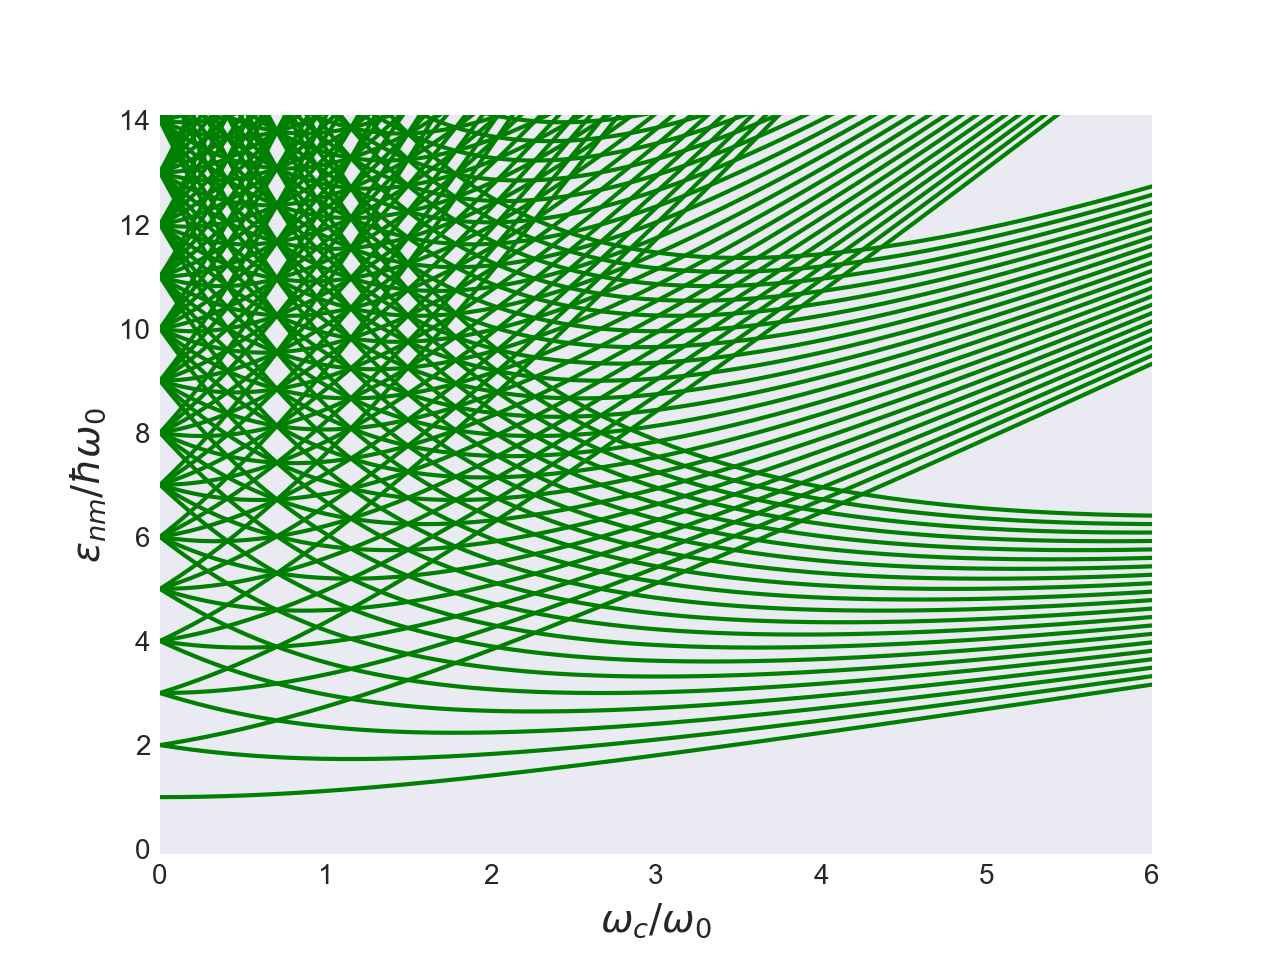
\includegraphics[width=0.75\textwidth]{implementation/figures/spaghetti.png}
    \caption{A few of the lowest eigenvalues $\epsilon_{nm}$ for a two-dimensional 
    quantum dot for transverse magnetic field of increasing strength. This plot of 
    the single-particle energies form the Fock-Darwin spectrum. Some states for very 
    high values of $m$ are omitted to make the formation of Landau bands in strong
    fields more visible.
    \label{fig:magnetic_spaghetti}}
\end{figure}

Notice in \autoref{fig:magnetic_spaghetti}, that there are lengthy intervals of 
b-field strength were there is no degeneracy in the eigenenergies. Conversely, there 
for certain specific field strengths there are very interesting shell structures with 
diverse energies. For $\omega_c/\omega=1/\sqrt{2}$ we get the interesting shell structure
depicted in \autoref{fig:b_field_degeneracy}. Such accidental bunching also occurs 
for $\omega_c/\omega=2/\sqrt{3}, 3/2, 4/\sqrt{5}\dots$. We also see from figure 
\autoref{fig:magnetic_spaghetti} that for an infinitely strong magnetic field as 
$\omega_c/\omega \to \infty$, in the free particle limit, that the energy levels 
form a sequence of so-called Landau bands. 


\begin{figure}
    \centering
    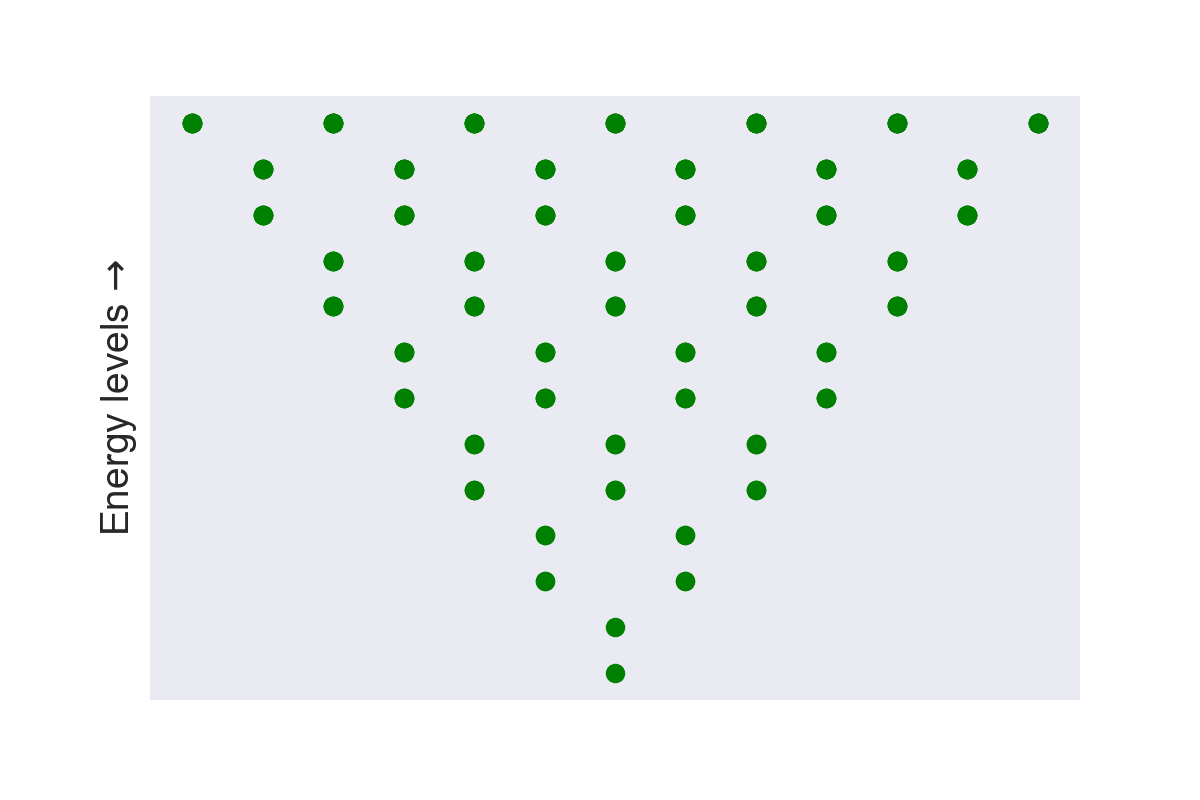
\includegraphics[width=0.75\textwidth]{implementation/figures/omega_inv_square_root_2_degeneracy.png}
    \caption{Illustration of eigenenergy degeneracies for two-dimensional quantum 
    dot for transverse magnetic field of strength $\omega_c=1/\sqrt{2}$.
    Each dot 
    \label{fig:b_field_degeneracy}}
\end{figure}

As for the computation of the basis set, not much needs to be added in the computation 
than the extra energy to the diagonal part of the one-body matrix elements $h^p_q$, as 
everything else is the same, including the two-body Coulomb integrals. But, as we have 
already mentioned and displayed in \autoref{fig:magnetic_spaghetti}, for increasing 
strength of the magnetic field, the eigenenergies as function  of $\omega_c$ eventually 
cross over one another. The magnetic field has the effect of decreasing the energy of
a state with $m>0$ and increasing the energy of a state with $m<0$. This means that 
it is necessary to sort the eigenvalues after they have been computed. 

The class specification of the two-dimensional quantum dot subjected to a transverse,
homogeneous, static magnetic field is below.

\begin{tcolorbox}
    {\fontfamily{cmss}\selectfont
    \textbf{class} quantum\_systems.\textbf{TwoDimHarmonicOscB}

    \hspace{1em}(\emph{n}, \emph{l}, \emph{radius\_length}, \emph{num\_grid\_points}, 
    \emph{omega\_0=$1.0$}, \emph{mass=$1$}, \emph{omega\_c=$0$})

    \vspace{1em}
    Create Two-Dimensional Quantum Dot with constant homogenous magnetic field.
    This class inherits from \textbf{TwoDimensionalHarmonicOscillator}.
    \vspace{1em}

    \textbf{Parameters}

    \hspace{2em}\textbf{n}(\emph{int}) Number of electrons
    
    \hspace{2em}\textbf{l}(\emph{int}) Number of spinorbitals
    
    \hspace{2em}\textbf{grid\_length}(\emph{int or float}) Space over which to 
        construct wavefunction.
    
    \hspace{2em}\textbf{num\_grid\_points}(\emph{int of float}) Number of 
        points for wavefunction.

    \hspace{2em}\textbf{omega\_0}(\emph{float, default $1.0$}) Part of harmonic 
        osc. not dep. on magnetic field. 
    
    \hspace{2em}\textbf{mass}(\emph{int or float, default $1.0$}) Mass of electrons.
        Atomic units is used as default.
    
    \hspace{2em}\textbf{omega\_c}(\emph{float, default $0$}) Larmor frequency.

    \vspace{1em}
    \textbf{Attributes}

    \hspace{2em} \textbf{h}
    One-body matrix 
    \textbf{Type} np.array
    
    \hspace{2em} \textbf{f}
    Fock matrix
    \textbf{Type} np.array

    \hspace{2em} \textbf{u}
    Two-body matrix
    \textbf{Type} np.array

    \vspace{1em}
    \textbf{Methods}

    \hspace{2em} \textbf{setup\_system}()
        \begin{adjustwidth}{4em}{}
        Must be called in order to compute basis functions.
        \end{adjustwidth}

    \hspace{2em} \textbf{construct\_dipole\_moment}()
        \begin{adjustwidth}{4em}{}
        Constucts dipole moment. This method is called by setup\_system().
        \end{adjustwidth}
    }
\end{tcolorbox}


\section{[UNFINISHED] Constructing a Custom System}

\section{[UNFINISHED] Time Evolution}


        \chapter{Coupled Cluster}

The main product of this study is manifested in the \lstinline{coupled_cluster}
module for Python. This module is designed to fit together with the
\lstinline{quantum_systems} module described in the previous chapter. We have tried to 
make this module easy to extend, resulting in a framework where every solver scheme 
inherits from an abstract parent class that specifies what must be implemented in order 
to make a supplemental solver or class operational in conjunction with the rest of the 
framework.

As a beginning to this project, which we hope will continue to grow and be used, 
we have implemented several different ground state solver classes, and several
time-dependent solver classes. In order of increasing sophistication and 
elegance, we have a ground state- and a time-dependent solver for both the coupled cluster
method
with double excitations (CCD), the coupled cluster method with singles- and double 
excitations (CCSD), and for the orbital-adaptive coupled cluster method with double
excitations (OACCD). The time-dependent solvers within a particular category are 
dependent on its ground state counterpart, but the ground state solvers can be used
independently.

The \lstinline{coupled_cluster} module can be install from github via \lstinline{pip}
by the following command,
\begin{lstlisting}[language=bash]
pip install git+https://github.com/Schoyen/coupled-cluster.git
\end{lstlisting}
If one prefers, the same task can be accomplished by the following commands,
\begin{lstlisting}[language=bash]
git clone https://github.com/Schoyen/coupled-cluster.git
cd coupled-cluster
pip install .
\end{lstlisting}
We have supplied environment specifications for \lstinline{conda}, with requirement 
specifications for the convenience of the user. Assuming the git repository is cloned 
properly,
\begin{lstlisting}[language=bash]
conda environment create -f environment.yml
\end{lstlisting}
Activate the environment with,
\begin{lstlisting}[language=bash]
conda activate cc
\end{lstlisting}
Full documentation of this module, which we hope will be kept up to date with any future revisions 
can be found at \url{www.coupled-cluster.com}.

\section{Ground State Computations}

    Before any development in time can be performed, we need to derive configurations 
    of systems that 
    we can be pretty certain exist in nature. This makes the implementation of ground 
    state solvers necessary. We have implemented ground state solvers; the
    \lstinline{CoupledClusterDoubles} and \lstinline{CoupledClusterSinglesDoubles} 
    are based on the theoretical framework form of the Lagrangian formulation of coupled 
    cluster, while \lstinline{OATDCCD} is a ground state version of an orbital-adaptive 
    ground state coupled cluster solver with double excitations. Moreover, we constructed 
    a data structure for the amplitudes in the \lstinline{AmplitudeContainer} class and 
    we have implemented two ``mixer'' classes that help with convergences of the ground
    state solvers, \lstinline{AlphaMixer} and \lstinline{DIIS}.

    \subsection{Representation of Amplitudes}

    The most central structure in any coupled cluster solver are the amplitudes. The 
    amplitudes are what defines the true structure of the wavefunction as a linear 
    combination of single-particle functions contained in the reference Slater 
    determinant. We have found it beneficial to implement a special container 
    class for the amplitudes, aptly called \lstinline{AmplitudeContainer}.

    \begin{tcolorbox}
    {\fontfamily{cmss}\selectfont
    \textbf{class} coupled\_cluster.cc\_helper.\textbf{AmplitudeContainer}
    (\emph{t}, \emph{l}, \emph{np})

    \vspace{1em}
    Container for amplitude functions.

    \vspace{1em}
    \textbf{Parameters:}

    \hspace{2em}\textbf{t}(\emph{list}, \emph{tuple}, \emph{set}) $\tau$ amplitudes

    \hspace{2em}\textbf{l}(\emph{list}, \emph{tuple}, \emph{set}) $\lambda$ amplitudes

    \hspace{2em}\textbf{np}(\emph{module}) Matrix library, e.g. numpy, cupy etc

    \vspace{1em}
    \textbf{Attributes:}

    \hspace{2em} \textbf{t} $\tau$ amplitudes

    \hspace{2em} \textbf{l} $\lambda$ amplitudes

    \vspace{1em}
    \textbf{Methods:}

    \hspace{2em} \textbf{unpack}()
    \begin{adjustwidth}{4em}{}
        \textbf{Returns:} Amplitudes

        \textbf{Return type:} \emph{generator}
    \end{adjustwidth}

    \hspace{2em} \textbf{asarray}()
    \begin{adjustwidth}{4em}{}
        \textbf{Returns:} Amplitude vector

        \textbf{Return type:} \emph{np.array}
    \end{adjustwidth}

    }
\end{tcolorbox}

    The \lstinline{AmplitudeContainer} class is built as a data structure for 
    the amplitude functions, and comprises all methods and attributes to serve this 
    purpose. This includes overloading of primitive methods of the base 
    python \lstinline{Object} type.: \lstinline{__add__} and \lstinline{__radd__}
    enables adding a scalar or properly shaped vector to the amplitudes, 
    \lstinline{__mul__} and \lstinline{__rmul__} allows for multiplication 
    with scalars and vectors, and \lstinline{__iter__} is implemented to make 
    the class an iterable. In summary, the \lstinline{AmplitudeContainer} 
    functions as a fully operational data structure for amplitudes of coupled 
    cluster solver, with both $\tau$ and $\lambda$ amplitudes.

    \subsection{Coupled Cluster Base Class}

    All ground state solvers within the \lstinline{coupled_cluster} module are built 
    as sub-classes of the abstract base class \lstinline{CoupledCluster}. The most
    important method of this class is the \lstinline{compute_ground_state()} method.
    This method in turn calls the \lstinline{iterate_t_amplitudes()} and 
    \lstinline{iterate_l_amplitudes()} successively. 

    As we have outlined in 
    \autoref{ch:coupled_cluster_theory}, the $\tau$ amplitudes are only dependent on 
    $\tau$, while the $\lambda$ amplitudes are dependent on both $\tau$ and $\lambda$.
    Therefore, the $\tau$ amplitude equations iterative solver
    \lstinline{iterate_t_amplitudes()} is called first, and the $\lambda$ amplitude
    equation solver is called second.
    For illustration, the most important section of the \lstinline{compute_l_amplitudes()} method 
    is the following
    \begin{python}
    for i in range(max_iterations):
    self.compute_l_amplitudes()
    residuals = self.compute_l_residuals()

    if self.verbose:
        print(f"Iteration: {i}\tResiduals (l): {residuals}")

    if all(res < tol for res in residuals):
        break

    assert i < (
        max_iterations - 1
    ), f"The l amplitudes did not converge. Last residual: {residuals}" 
    \end{python}
    The equivalent section of code in the \lstinline{compute_t_amplitudes()} method is 
    nearly identical.
    The \lstinline{CoupledCluster} class is supposed to provide a framework for which 
    to implement various coupled cluster ground state solver classes. It therefore
    has several abstract methods that such subclasses need to implement and overwrite.
    The most important of these are the methods \lstinline{compute_t_amplitudes} 
    and \lstinline{compute_l_amplitudes}, which are supposed to contain the evaluation 
    of amplitude equations for a given coupled cluster truncation and scheme. 

    With the hope that the functiunality of the rest of the methods 
    in the abstract base class \lstinline{CoupledCluster} can be inferred from 
    name, and with the goal of brevity we proceed to a study of the simplest 
    ground state coupled cluster solver, namely CCD, implemented in the 
    \lstinline{CoupledClusterDoubles} class. 

    \begin{tcolorbox}
    {\fontfamily{cmss}\selectfont
    \textbf{class} coupled\_cluster.cc.\textbf{CoupledCluster}

    \hspace{1em}(\emph{system}, \emph{mixer=<class'coupled\_cluster.mix.DIIS'>}, 
        \emph{verbose=False}, \emph{np=None})

    \vspace{1em}
    Abstract base class defining the basic structure of a coupled cluster ground state 
    solver class.
    
    \vspace{1em}
    \textbf{Parameters}

    \hspace{2em}\textbf{system}(\emph{QuantumSystem}) A system class from the 
        \emph{quantum\_systems} module.

    \hspace{2em}\textbf{mixer}(\emph{AlphaMixer, default AlphaMixer}) Mixer - 
        Subclass of \emph{AlphaMixer} class.

    \hspace{2em}\textbf{verbose}(\emph{bool, default False}) Will print results 
        for each iteration if \emph{True}.

    \vspace{1em}
    \textbf{Methods}

    \hspace{2em} \textbf{compute\_ground\_state}
        (\emph{t\_args=[]}, \emph{t\_kwargs=\{\}}, \emph{l\_argys=[]}, \emph{l\_kwargs=\{\}})
        \begin{adjustwidth}{4em}{}
        Computes ground state of system given as parameter. Allows for parameters relating 
        the the $\tau$- and $\lambda$ amplitudes, for use in inheriting classes.
        \end{adjustwidth}
    
    \hspace{2em} \textbf{compute\_particle\_density}()
        \begin{adjustwidth}{4em}{}
        Computes the one-body density of the system.
   
        \textbf{Returns:} Particle density 
  
        \textbf{Return type:} \emph{np.array}
        \end{adjustwidth}
    
    \hspace{2em} \textbf{compute\_reference\_energy}()
        \begin{adjustwidth}{4em}{}
        Computes reference energy

        \textbf{Returns:} Reference energy

        \textbf{Return type:} \emph{np.array}
        \end{adjustwidth}
    
    \hspace{2em} \textbf{get\_amplitudes}(\emph{get\_t\_0=False})
        \begin{adjustwidth}{4em}{}
        Getter for amplitudes.

        \textbf{Parameters:} 
        
            \hspace{1.5em} \textbf{get\_t\_0} (\emph{bool, default False}) 
            Returns amplitude at $t=0$ if \lstinline{True}.

        \textbf{Returns:} Amplitudes

        \textbf{Return type:} \emph{AmplitudeContainer}

        \end{adjustwidth}

    \hspace{2em} \textbf{iterate\_l\_amplitudes} 
        (\emph{max\_iterations=$100$}, \emph{tol=$1e^{-4}$}, \emph{**mixer\_kwargs})
        \begin{adjustwidth}{4em}{}
            Finds solution to $\lambda$ amplitudes iteratively.

        \textbf{Parameters:} 
        
        \hspace{1.5em} \textbf{max\_iterations} (\emph{int})
            The limit of iterations allowed.

        \hspace{1.5em} \textbf{tol} (\emph{float, default $1e^{-4}$})
            The tolerance for convergence.

        \end{adjustwidth}
 
    \hspace{2em} \textbf{iterate\_t\_amplitudes} 
        (\emph{max\_iterations=$100$}, \emph{tol=$1e^{-4}$}, \emph{**mixer\_kwargs})
        \begin{adjustwidth}{4em}{}
            Finds solution to $\tau$ amplitudes iteratively.

        \textbf{Parameters:} 
        
        \hspace{1.5em} \textbf{max\_iterations} (\emph{int})
            The limit of iterations allowed.

        \hspace{1.5em} \textbf{tol} (\emph{float, default $1e^{-4}$})
            The tolerance for convergence.

        \end{adjustwidth}
        
    \hspace{2em} \textbf{\_get\_t\_copy} Abstract method

    \hspace{2em} \textbf{\_get\_l\_copy} Abstract method

    \hspace{2em} \textbf{compute\_energy} Abstract method

    \hspace{2em} \textbf{compute\_one\_body\_density\_matrix} Abstract method

    \hspace{2em} \textbf{compute\_t\_amplitudes} Abstract method

    \hspace{2em} \textbf{compute\_l\_amplitudes} Abstract method

    \hspace{2em} \textbf{setup\_t\_mixer} Abstract method

    \hspace{2em} \textbf{setup\_l\_mixer} Abstract method

    \hspace{2em} \textbf{compute\_t\_residuals} Abstract method

    \hspace{2em} \textbf{compute\_l\_residuals} Abstract method

    }
\end{tcolorbox}

    \subsection{Coupled Cluster Doubles}
    
    Starting from construction, the \lstinline{CoupledClusterDoubles} class passes 
    the system, defined through a \lstinline{QuantumSystem} object to the 
    parent class constructor, along with any keyword arguments, such as turning 
    on verbosity, mixer type and what matrix library to apply. The
    \lstinline{QuantumSystem} class will contain all the information necessary to 
    set up the system, i.e. construct a one-body matrix, fock matrix and two-body 
    matrix. These will be used to set up empty arrays for the $\tau$ and $\lambda$ 
    amplitudes. The \lstinline{compute_initial_guess} is called lastly in the 
    constructor, computing the inital guess of the double-excited amplitudes as 
    \begin{equation}
        \label{eq:ccd_inital_guess}
        \tau^{(0)} = \frac{u^{ab}_{ij}}{D^{ab}_{ij}},
    \end{equation}
    where $u$ is the two-body operator and
    $D^{ab}_{ij} = f^a_a + f^b_b - f^i_i - f^j_j$,
    where $f$ is the Fock operator.
    
    In the \lstinline{CoupledClusterDobles} class specification one would
    notice that it has implementations of all the abstract methods 
    from the \lstinline{CoupledCluster} abstract class. The reason for the existence 
    of the class, the \lstinline{compute_ground_state()} method, is inherited from the 
    parent class, and does the same thing as described above - calling 
    \lstinline{iterate_t_amplitudes()} and \lstinline{iterate_l_amplitudes()}. These 
    methods also exist as members of \lstinline{CoupledClusterDoubles}, but are excluded 
    from the class specification for sake of brevity. It is 
    possible to pass arguments to the the two iterator methods; one list for each iteration
    method, or as keywords.
    One can also pass arguments 
    to the mixer through the \lstinline{compute_ground_state_method()}. 
    An overview of mixing applied to iterative solvers is given in the next 
    section.

    The important part of the specific coupled cluster scheme solver is contained in the two 
    methods \lstinline{compute_t_amplitudes()} and \lstinline{compute_l_amplitudes()}.
    These functions evaluate the entire coupled cluster doubles amplitude equations.
    The computation of each term (diagram) in the amplitude equation is done in separate functions,
    as calls to \lstinline{numpy.tensordot()}, for a total of ten terms for the 
    $\tau$ amplitude equation in the coupled cluster doubles method including 
    permutation operators:
    \begin{equation}
        \label{eq:ccd_tau}
        \begin{aligned}
        0 =& u^{ab}_{ij} + f^b_c \tau^{ac}_{ij}P(ab) 
            - f^k_j \tau^{ab}_{ik}P(ij)
            + \frac{1}{4} \tau^{ac}_{ij} \tau^{ab}_{mn}u^{mn}_{cd} 
            + \frac{1}{2} \tau^{cd}_{ij}u^{ab}_{cd}
            + \frac{1}{2} \tau^{cd}_{jm} \tau^{ab}_{in} u^{mn}_{cd}P(ij) \\
            &\ - \frac{1}{2} \tau^{ac}_{nm} \tau^{bd}_{ij} u^{nm}_{cd}P(ab)
            + \tau^{ac}_{im} \tau^{bd}_{jn}u^{mn}_{cd}P(ij)
            + \tau^{ac}_{im}u^{bm}_{jc}P(ab)P(ij)
            + \frac{1}{2} \tau^{ab}_{mn}u^{mn}_{ij}.
        \end{aligned}
    \end{equation}

    The initial guess in equation \autoref{eq:ccd_inital_guess} is terms 2 and 3
    from \autoref{eq:ccd_tau}. These terms also form the basis of the iterative scheme,
    if we move them to the left of the equal sign in \autoref{eq:ccd_tau}, 
    \begin{equation}
        D^{ab}_{ij} \tau^{ab}_{ij} = g(u, \tau),
    \end{equation}
    where $g(u, \tau)$ now consists of the rest of the doubles amplitude equation, our 
    recursion relation can be written
    \begin{equation}
        t^{(k+1)} = \frac{g(u,\tau^{(k)})}{D^{ab}_{ij}}.
    \end{equation}

    \begin{tcolorbox}
    {\fontfamily{cmss}\selectfont
    \textbf{class} coupled\_cluster.cc.\textbf{CoupledClusterDoubles}
    (\emph{system}, \emph{**kwargs})

    \vspace{1em}
    Implementation of coupled cluster with double excitations ground state solver. 
    Inherits from the \textbf{CoupledCluster} abstract base class.

    \vspace{1em}
    \textbf{Parameters}

    \hspace{2em}\textbf{system}(\emph{QuantumSystem}) A system class from the 
        \emph{quantum\_systems} module.

    \vspace{1em}
    \textbf{Methods} 
 
    \hspace{2em} \textbf{compute\_ground\_state}
        (\emph{t\_args=[]}, \emph{t\_kwargs=\{\}}, \emph{l\_args=[]}, \emph{l\_kwargs=\{\}})
        \begin{adjustwidth}{4em}{}
        Computes CCD ground state of given system.
        \end{adjustwidth}  

    \hspace{2em} \textbf{compute\_initial\_guess}()
        Computes initial guess for amplitudes.
        %\begin{adjustwidth}{4em}{}
        %\end{adjustwidth}

    \hspace{2em} \textbf{\_get\_t\_copy}()
        \begin{adjustwidth}{4em}{}
        \textbf{Returns:} Copy of $\tau^{ab}_{ij}$ amplitudes
        
        \textbf{Return type:} \emph{AmplitudeContainer}
        \end{adjustwidth}

    \hspace{2em} \textbf{\_get\_l\_copy}()
        \begin{adjustwidth}{4em}{}
        \textbf{Returns:} Copy of $\lambda^{ij}_{ab}$ amplitudes
        
        \textbf{Return type:} \emph{AmplitudeContainer}
        \end{adjustwidth}

    \hspace{2em} \textbf{compute\_t\_residuals}()
        \begin{adjustwidth}{4em}{}
        \textbf{Returns:} Norm of $\tau^{ab}_{ij}$ amplitudes
        
        \textbf{Return type:} \emph{float}
        \end{adjustwidth}

    \hspace{2em} \textbf{compute\_l\_residuals}()
        \begin{adjustwidth}{4em}{}
        \textbf{Returns:} Norm of $\lambda^{ij}_{ab}$ amplitudes
        
        \textbf{Return type:} \emph{float}
        \end{adjustwidth}

    \hspace{2em} \textbf{setup\_t\_mixer}(\emph{**kwargs})
        Sets up mixer for $\tau$ amplitudes

    \hspace{2em} \textbf{setup\_l\_mixer}(\emph{**kwargs})
        Sets up mixer for $\lambda$ amplitudes

    \hspace{2em} \textbf{compute\_energy}()
        \begin{adjustwidth}{4em}{}
        \textbf{Returns:} CCD ground state energy

        \textbf{Return type:} {\emph{float}}
        \end{adjustwidth}

    \hspace{2em} \textbf{compute\_t\_amplitudes}()
        Computes $\tau$ amplitudes

    \hspace{2em} \textbf{compute\_l\_amplitudes}()
        Computes $\lambda$ amplitudes
    
    \hspace{2em} \textbf{compute\_one\_body\_density}()
        \begin{adjustwidth}{4em}{}
        \textbf{Returns:} One-body density matrix

        \textbf{Return type:} \emph{np.array}
        \end{adjustwidth}

    \hspace{2em} \textbf{compute\_two\_body\_density}()
        \begin{adjustwidth}{4em}{}
        \textbf{Returns:} Two-body density matrix

        \textbf{Return type:} \emph{np.array}
        \end{adjustwidth}

    }
\end{tcolorbox}
    \vfill
    \pagebreak

    An example of a computation of one term from \autoref{eq:ccd_tau} is,
    \begin{python}
    def add_d2e_t(u, t, o, v, out, np):
        term = np.tensordot(t, u[o, v, v, o], axes=((1, 3), (2, 0)))
            .transpose(
                0, 2, 1, 3
        )
        term -= term.swapaxes(0, 1)
        term -= term.swapaxes(2, 3)
        out += term
    \end{python}
    This function particular computes the $D_{2e}$ diagram\footnote{After the labelling from 
    \autoref{ch:coupled_cluster_theory} and Shavitt \& Bartlett\cite{shavitt2009many}}.

    \subsection{Coupled Cluster Singles Doubles}

    Most of the rest of the methods in the \lstinline{CoupledClusterDoubles} class are there 
    for the use of other methods, or for extracting observables. Moving to the next logical 
    coupled cluster solver scheme; the coupled cluster method with single- and double 
    excitations is now a matter of taking into account the extra computations needed in 
    this scheme, for each method in the abstract base clase \lstinline{CoupledCluster}. 
    There are indeed many more computations, but the code will structurally be the same. 
    The class specification for \lstinline{CoupledClusterSinglesDoubles} is therefore 
    given here without specification of the methods as they are excactly the same. For testing 
    purposes, the \lstinline{CoupledClusterSingelsDoubles} class have the option 
    to only include double excitation at construction. The amplitude equations for 
    the CCSD scheme is found by constructing the coupled cluster Lagrangian
    (\autoref{eq:cc_energy_lagrangian}) in \lstinline{sympy} and differentiating 
    it symbolically. The resulting equations can be found in \autoref{app:ccsd_equations}.

    \begin{tcolorbox}
    {\fontfamily{cmss}\selectfont
    \textbf{class} coupled\_cluster.cc.\textbf{CoupledClusterSinglesDoubles}

    \hspace{1em}(\emph{system}, \emph{include\_singles=True}, \emph{**kwargs})

    \vspace{1em}
    Implementation of coupled cluster with single- and double excitations
    ground state solver. 
    Inherits from the \textbf{CoupledCluster} abstract base class.
    \vspace{1em}

    \textbf{Parameters}

    \hspace{2em}\textbf{system}(\emph{QuantumSystem}) A system class from the 
        \emph{quantum\_systems} module.

    \hspace{2em}\textbf{include\_singles}(\emph{bool, default True}) 
        Includes single excitations if \lstinline{True}.
    } 
\end{tcolorbox}

    \subsection{Orbital-Adaptive Coupled Cluster}

    The algorithm applied when computing the ground state in the orbital-adaptive sphere 
    is the nonorthogonal orbital-optimised coupled cluster (NOCC) method, developed by 
    Myhre\cite{myhre2018demonstrating}. The NOCC scheme is shown to converge towards full
    configuration interaction. Since the \lstinline{OACCD} class is acutally applying 
    NOCC it can be perceived as a misnomer, but as of yet there exist no ground state 
    equivalent of the time-dependent 
    orbital-adaptive coupled cluster (OACC) method. Such a method is in development, and there
    is strong indication that NOCC would be equivalent to a OACC ground state solver. What is 
    more, NOCC does vary the orbitals as well as iterate over amplitude, and we have therefore 
    opted to call it OACC.

    \begin{tcolorbox}
    {\fontfamily{cmss}\selectfont
    \textbf{class} coupled\_cluster.cc.\textbf{OACCD}
    (\emph{system}, \emph{**kwargs})

    \vspace{1em}
    Implementation of the orbital-adaptive coupled cluster method with double excitation,
    also called the nonorthogonal orbital-optimized coupled cluster model.
    Requires orthonormal basis functions. Based on work by Rolf H. 
    Myhre\cite{myhre2018demonstrating}.

    Inherits from the \textbf{CoupledCluster} abstract base class.

    \vspace{1em}
    \textbf{Parameters}

    \hspace{2em}\textbf{system}(\emph{QuantumSystem}) A system class from the 
        \emph{quantum\_systems} module.

    \vspace{1em} 
    \textbf{Methods}

    \hspace{2em} \textbf{compute\_ground\_state}
        (\emph{max\_iterations=$100$}, \emph{tol=$1e^{-4}$},

        \hspace{3em} \emph{termination\_tol=$1e^{-4}$}, \emph{tol\_factor=$0.1$},
        \emph{change\_system\_basis=False},
        
        \hspace{3.2em}\emph{**mixer\_kwargs})

        \begin{adjustwidth}{4em}{}
        Computes ground state of system.

        \textbf{Parameters:} 

            \hspace{1.5em}\textbf{max\_iterations} (\emph{int, default $100$}) 
            Maximum number of iterations.

            \hspace{1.5em}\textbf{tol} (\emph{float, default $1e^{-4}$})
            Tolerance of convergence.

            \hspace{1.5em}\textbf{termination\_tol} (\emph{float, default $1e^{-4}$})
            Give up if tolerance is below this.

            \hspace{1.5em}\textbf{tol\_factor} (\emph{float, default $0.1$})
            Decreases tolerance if non-convergent.

            \hspace{1.5em}\textbf{change\_system\_basis} (\emph{bool, default False})
            Changes basis after calculation.

        \end{adjustwidth}
    } 
\end{tcolorbox}

    Our implementation of the NOCC ground state solver is inherited from code written by
    \citeauthor{myhre2018demonstrating} and 
    adapted to our 
    framework. We supply a brief overview of the algorithm here. The starting point for the 
    NOCC model is the bivariational Lagrangian
    \begin{equation}
        \label{eq:nocc_lagrangian}
        \mathscr{L} = \mel*{\tilde{\Psi}}{\hat{H}}{\Psi} \\
            = \mel*{\tilde{\phi}}
                {
                (1 + \Lambda) e^{-\hat{T}}e^{-\kappa}\hat{H}e^{\kappa}e^{\hat{T}}
                }{\phi}
    \end{equation}
    which is very similar to the coupled cluster Lagrangian (\autoref{eq:cc_energy_lagrangian}),
    except for a biorthogonal basis and a transformation of the Hamiltonian, defined 
    as follows
    \begin{equation}
        \begin{aligned}
            \tilde{c}_p^\dagger &= e^{-\kappa}\hat{c}_p^\dagger e^\kappa \\
            c_p &= e^{-\kappa} \hat{c}_p^\dagger e^\kappa \\
            \ket{\phi} &= e^{-\kappa}\ket*{\hat{\phi}}
        \end{aligned}
    \end{equation}
    where the orthogonal reference creation- and annihilation operators marked with a hat
    ($\hat{\ }$), as is the reference state function. We require that $\kappa$ is antihermitian,
    \begin{equation}
        \kappa = \sum_{pq} \kappa_{pq}c^\dagger_p c_q, \quad \kappa^\dagger = -\kappa.
    \end{equation}
    Moreover, we split $\kappa$ into excitations and relaxations (up and down),
    \begin{equation}
        \label{eq:agg_kappa}
        \kappa = \sum_{ai} \kappa^u_{ai}c^\dagger_a \tilde{a}_i
            + \kappa^d_{ia} c^\dagger_i \tilde{c}_a
            = \sum_{ai} \kappa^u_{ai} X_ai + \kappa^d_{ia} \tilde{X}^\dagger_{ia}.
    \end{equation} 
    
    As in any many-body formulation that includes a Lagrangian, we would like to compute 
    the first-order conditions of the Lagrangian, in order to derive what would be the 
    NOCC equation. The problem with this is that the result would be some extremely 
    lengthy expressions, because $\kappa$ does not commute with $\hat{T}$ or $\Lambda$.
    Therefore, we express the NOCC equations with an optimized basis where $\kappa=0$,
    where a solution would correspond to a stationary point of the Schrödinger equation.
    This is the same as expanding the exponentials in $\kappa$ and keeping only zero-order 
    terms. This trick leads to an algorithm which iterates between orbital transformations 
    and amplitudes until self-consistency.

    At a particular stationary point the differential of the Lagrangian
    (\autoref{eq:nocc_lagrangian}) must be zero with respect to the four sets of 
    parameters $\{\tau\}$, $\{\lambda\}$, $\{\kappa^u\}$ and $\{\kappa^d\}$, giving
    us four sets of equations,
    \begin{align}
        \frac{\partial \mathscr{L}}{\partial \lambda_{\mu_n}}
            &= \mel*{\tilde{\phi}}
            {\tilde{X}_{\mu_n} e^{-\hat{T}}\hat{H}e^{\hat{T}}}
            {\phi}, \\
        \frac{\partial \mathscr{L}}{\partial \tau_{\mu_n}}
            &= \mel*{\tilde{\phi}}
            {(1 + \Lambda)e^{-\hat{T}}[\hat{H}, X_{\mu_n}]e^{\hat{T}}}
            {\phi}, \\
        \frac{\partial \mathscr{L}}{\partial \kappa^u_{\mu_1}}
            &= \mel*{\tilde{\phi}}
            {(1 + \Lambda)e^{-\hat{T}}[\hat{H}, X_{\mu_1}]e^{\hat{T}}}
            {\phi}, \\
        \frac{\partial \mathscr{L}}{\partial \kappa^d_{\mu_1}}
            &= \mel*{\tilde{\phi}}
            {(1 + \Lambda)e^{-\hat{T}}[\hat{H}, \tilde{X}_{\mu_1}]e^{\hat{T}}}
            {\phi}.
    \end{align}

    We are now ready to outline the full algorithm of the 
    \lstinline{compute_ground_state()} in what we have called the \lstinline{OACCD}.
    The method is iterating over the the norm of $\kappa^u$ and $\kappa^d$, called the 
    residuals of $\kappa$, until consistency compared to a tolerance value is achieved. 
    For each such iteration, iteration over the $\tau$ and $\lambda$ double excitation
    amplitudes is performed, but at a much less strict tolerance value than under the 
    \lstinline{CoupledClusterDoubles} scheme. After the iteration over $\tau$ and $\lambda$ 
    is achieved, the values for $\kappa^u$ and $\kappa^d$ are recalculated, in order to 
    compute the aggragate $\kappa$ (\autoref{eq:agg_kappa}), 
    which in turn can be used to transform the orbitals,
    \begin{equation*}
        \begin{gathered}
            h^{(k + 1)} = e^{-\kappa} h^{(k)} e^{\kappa}, \\
            (u^{pq}_{rs})^{(k + 1)}
            = (e^{-\kappa})^p_a (e^{-\kappa})^q_b 
                (u^{ab}_{cd})^{(k)}
            (e^{\kappa})^d_s (e^{\kappa})^c_r,
        \end{gathered}
    \end{equation*}
    which (in addition to being written with incomprehensible notation) is used to compute 
    a new Fock operator. The resulting rotation of the orbitals will aid in better 
    convergence towards the ground state.

    \subsubsection{Specialised Orbital-Adaptive \lstinline{AmplitudeContainer}}

    Because of the nature of the orbital-adaptive coupled cluster scheme, it is no 
    longer sufficient to store just the amplitudes as representation of the exact 
    state. Therefore, we have implemented a subclass of the \lstinline{AmplitudeContainer}
    data structure which also contains the coefficient matrices necessary to perform the 
    required orbital transformations.

    \begin{tcolorbox}
    {\fontfamily{cmss}\selectfont
    \textbf{class} coupled\_cluster.cc\_helper.\textbf{OACCVector}
    (\emph{t}, \emph{l}, \emph{C}, \emph{C\_tilde} \emph{np})

    \vspace{1em}
    Container for amplitude functions.

    \vspace{1em}
    \textbf{Parameters:}

    \hspace{2em}\textbf{t}(\emph{list}, \emph{tuple}, \emph{set}) $\tau$ amplitudes

    \hspace{2em}\textbf{l}(\emph{list}, \emph{tuple}, \emph{set}) $\lambda$ amplitudes

    \hspace{2em}\textbf{C}(\emph{np.array}) Right-hand side coefficient matrix

    \hspace{2em}\textbf{C\_tilde}(\emph{np.array}) Left-hand side coefficient matrix

    \hspace{2em}\textbf{np}(\emph{module}) Matrix library, e.g. numpy, cupy etc

    \vspace{1em}
    \textbf{Attributes:}

    \hspace{2em} \textbf{t} $\tau$ amplitudes

    \hspace{2em} \textbf{l} $\lambda$ amplitudes

    \hspace{2em} \textbf{C} Coefficient matrix $\vb{C}$ 

    \hspace{2em} \textbf{C\_tilde} Coefficient matrix $\tilde{\vb{C}}$

    \vspace{1em}
    \textbf{Methods:}

    \hspace{2em} \textbf{unpack}()
    \begin{adjustwidth}{4em}{}
        \textbf{Returns:} Amplitudes and coefficient matrices

        \textbf{Return type:} \emph{generator}
    \end{adjustwidth}

    \hspace{2em} \textbf{asarray}()
    \begin{adjustwidth}{4em}{}
        \textbf{Returns:} Amplitude vector and coefficient matrices

        \textbf{Return type:} \emph{np.array}
    \end{adjustwidth}

    }
\end{tcolorbox}

    Like the \lstinline{AmplitudeContainer} class, this data structure also implements 
    fuctionality for addition, multiplications and iteration.
    
\subsection{Mixing of Amplitude Vectors}

    Iterative many-body methods are prone to convergence problems for certain configurations.
    This would be doubly important since we have moved to a variational description 
    of coupled cluster theory,
    where generalisations of the variational theory dictate inifitesimal variations, which 
    is not always feasible to implement.
    Moreover, an iterative optimisation scheme may not always converge properly at all. 
    Luckily, there exists numerous techniques both for controlling and acceleration 
    convergence.

    \subsubsection{Alpha mixer}

    The simplest way to ``massage'' convergence out of the coupled cluster ground state methods
    to use a dampening, where one would include a part of the result from the previous 
    iteration, here applied to the $\tau$ amplitudes,
    \begin{equation}
        \bar{\tau}^{(k+1)} = (1 - \theta)\tau^{(k+1)} + \theta\tau^{(k)},
    \end{equation}
    where $\tau^{(k+1)}$ is the current result from evaluating the amplitude equations, 
    and $\tau^{(k)}$ is the previous value. Choosing $\theta \in [0,1]$ will tune how
    much of the previous amplitude to include in the new state. The idea is to allow for 
    a more gentle transition between the iterations. We have implemented this 
    very simple mixing scheme in the \lstinline{AlphaMixer} class, which also serves as 
    a base class for further mixer implementations.

    \begin{tcolorbox}
    {\fontfamily{cmss}\selectfont
    \textbf{class} coupled\_cluster.mix.\textbf{AlphaMixer}
    (\emph{theta=0.1}, \emph{np=None})

    \vspace{1em}
    Class defining the $\alpha$ mixer. Computes a superposition of current and new 
    amplitude vector. Also defines base class and methods the new mixer classes must
    implement.
        
    \vspace{1em}
    \textbf{Parameters}

    \hspace{2em}\textbf{theta}(\emph{float, default 0.1}) 
        Mixing parameter. $\theta \in [0, 1]$

    \hspace{2em}\textbf{np}(\emph{Module})
        Matrix library to be used, e.g. numpy, cupy.

    \vspace{1em} 
    \textbf{Methods}

    \hspace{2em} \textbf{compute\_new\_vector}
        (\emph{trial\_vector}, \emph{direction\_vector} \emph{error\_vector})

        \begin{adjustwidth}{4em}{}
        Computes new trial vector for mixing with full right hand side of amplitude 
        equation.

        \textbf{Parameters:} 

            \hspace{1.5em}\textbf{trial\_vector} (\emph{np.array}) 
            Initial vector for mixing

            \hspace{1.5em}\textbf{direction\_vector} (\emph{np.array})
            Vector to be added to \emph{trial\_vector}.

            \hspace{1.5em}\textbf{error\_vector} (\emph{np.array})
            Not used in $\alpha$ mixer. Needed in subclasses.

        \textbf{Returns:} New mixed vector

        \textbf{Return type:} \emph{np.array}

        \end{adjustwidth}
    } 
\end{tcolorbox}


    \subsubsection{The Quasi-Newton method with DIIS acceleration}

    A more sophisticated method to aid in convergence, and perhaps the most popular,
    is by performing a direct inversion of iterative subspace (DIIS). The DIIS method 
    is built to accelerate the quasi-Newton method, an we will necesarily outline the 
    quasi-Newton before we examine DIIS, which is explained in Helgaker et 
    al.\cite{helgaker2014molecular}.

    The commutator of Fock operator with the cluster operator is generally
    \begin{equation}
        \label{eq:fock_cluster_commutator}
        [\hat{f}, \hat{T}] = \sum_\mu D_\mu \tau_\mu X_\mu,
    \end{equation}
    where $\epsilon_\mu$ is the sum of unoccupied energies minus the sum of all 
    occupied energies, i.e. $D^{ab}_{ij} = \epsilon_a  + \epsilon_b - \epsilon_i - \epsilon_j$,
    $\tau_\mu$ is the amplitude of a particular excitation, and $X_\mu$ is an excitation 
    operator. For CCD \autoref{eq:fock_cluster_commutator} becomes,
    \begin{equation}
        [\hat{f}, \hat{T}_2] = D^{ab}_{ij} \tau^{ab}_{ij} c^\dagger_a c^\dagger_b c_i c_j.
    \end{equation}
    This allows us to write the coupled cluster vector function $\Omega^{(0)}_\mu$,
    and its Jacobian $\Omega^{(1)}_{\mu\nu}$ of the $n$th iteration in the form 
    \begin{align}
        \label{eq:vector_function_diis}
        \Omega^{(0)}_\mu &= D_\mu \tau^{(n)}_\mu 
            + \mel{\Phi_\mu}
            {e^{-\hat{T}^{(n)}} \hat{U} e^{\hat{T}^{(n)}}}
            {\Phi_0} \\
        \label{eq:jacobian_diis}
        \Omega^{(1)}_{\mu\nu} &= D_\mu\delta_{\mu\nu} 
            + \mel{\Phi_\mu}
            {e^{-\hat{T}^{(n)}} [\hat{U}, X^\nu] e^{\hat{T}^{(n)}}}
            {\Phi_0}
    \end{align}
    which are very similar to the coupled cluster energy and amplitude equations, but 
    the matrix element contains just $\hat{U}$, the fluctuation potential, instead of 
    the entire Hamiltonian $\hat{H} = \hat{F} + \hat{U}$.

    The Jacobian constists only of a diagonal part, involving differences of the 
    orbital energies, and a nondiagonal part, containing the fluctuation potential.
    The trick from \emph{Newton's} method is to expand the vector functions around 
    the set of amplitudes of the current iteration $\tau^{(n)}$,
    \begin{equation}
        \Omega(\tau^{(n)} + \Delta\tau) = \Omega^{(0)}(\tau^{(n)})
            + \Omega^{(1)}(\tau^{(n)})\Delta \tau + \dots,
    \end{equation}
    which leads to a recursion relation, neglecting terms that are nonlinear in
    $\Delta \tau$,
    \begin{equation}
        \Omega^{(1)}(\tau^{(n)})\Delta \tau^{(n)} = - \Omega^{(0)}(\tau^{(n)}).
    \end{equation}
    By inserting \autoref{eq:vector_function_diis} and \autoref{eq:jacobian_diis} 
    we get the \emph{quasi-Newton} equations for the optimisation of the 
    coupled-cluster wavefunction,
    \begin{equation}
        \label{eq:quasi_newton}
        \Delta \tau^{(n)}_\mu = - \frac{\Omega^{(0)}_\mu(\tau^{(n)})}{D_\mu}
    \end{equation}
    The quasi-Newton method is fairly robust, but the convergence may be improved 
    significantly by introducing DIIS.

    In the DIIS framework\cite{pulay1980convergence}, the new amplitudes 
    $\tau^{(n+1)}$ are obtained by a linear interpolation among the previous 
    estimates of the amplitudes,
    \begin{equation}
        \tau^{(n+1)} = \sum_{k+1}^n w_k(\tau^{(k)} + \Delta\tau^{(k)}),
    \end{equation}
    where $\Delta\tau^{(k)}$ are obtained from \autoref{eq:quasi_newton}, and 
    the interpolations weights sum to unity,
    \begin{equation*}
        \label{eq:diis_weights_sum}
        \sum_{k=1}^n w_k = 1.
    \end{equation*}
    To determine the DIIS weights, we associate each set of amplitudes $\tau^{(k)}$ 
    with an error vector. We use the scaled vector function $\Delta\tau^{(k)}$ as 
    error vector and determine the interpolation coefficients by minimising the norm of 
    the averaged vector
    \begin{equation}
        \Delta \tau^{\text{ave}} = \sum_{k=1}^n w_k \Delta \tau^{(k)}
    \end{equation}
    subject to \autoref{eq:diis_weights_sum}.

    We have implemented the DIIS acceleration of the quasi-Newton method in the class 
    \lstinline{DIIS}. This class inherits from the \lstinline{AlphaMixer} class and
    would function in its place. The \lstinline{DIIS} class allows one to pick 
    how many vectors to store and compute a linear interpolation of, with a default 
    value of $10$ vectors.

    \begin{tcolorbox}
    {\fontfamily{cmss}\selectfont
    \textbf{class} coupled\_cluster.mix.\textbf{DIIS}
    (\emph{theta=0.1}, \emph{np=None})

    \vspace{1em}
    General vector mixing class to accelerate quasi-Newton using the 
    direct inversion of iterative space (DIIS) scheme. Inherits from 
    \emph{AlphaMixer}.
        
    \vspace{1em}
    \textbf{Parameters}

    \hspace{2em}\textbf{num\_vecs}(\emph{float, default 0.1}) 
        Number of vectors to keep in memory.
    \hspace{2em}\textbf{np}(\emph{Module})
        Matrix library to be used, e.g. numpy, cupy.

    \vspace{1em} 
    \textbf{Methods}

    \hspace{2em} \textbf{compute\_new\_vector}
        (\emph{trial\_vector}, \emph{direction\_vector} \emph{error\_vector})

        \begin{adjustwidth}{4em}{}
        Computes new trial vector for mixing with full right hand side of amplitude 
        equation.

        \textbf{Parameters:} 

            \hspace{1.5em}\textbf{trial\_vector} (\emph{np.array}) 
            Initial vector for mixing

            \hspace{1.5em}\textbf{direction\_vector} (\emph{np.array})
            Vector to be added to \emph{trial\_vector}.

            \hspace{1.5em}\textbf{error\_vector} (\emph{np.array})
            Error vector associated with QN DIIS. 

        \textbf{Returns:} New mixed vector

        \textbf{Return type:} \emph{np.array}
        \end{adjustwidth}

    \hspace{2em} \textbf{clear\_vectors}()
        \begin{adjustwidth}{4em}{}
        Delete all stored vectors.
        \end{adjustwidth}
    } 
\end{tcolorbox}

    \vfill
    \pagebreak

\section{Time Development}

    We have sought to formulate the time-dependent coupled cluster methods
    in the abstraction of very general differential equations. By doing this we 
    conform to the mindset of \emph{implement once, apply anywhere}. In any 
    implementation of a time-dependent coupled cluster solver, we consider it as
    though we  are working with a general function $f(u(t), t)$, so that it can 
    be solved by any general solver for a differential equation. The abstract 
    formulation of a differential equation reads 
    \begin{equation}
        \label{eq:general_ode_orig}
        u'(t) = f(u(t), t).
    \end{equation}
    Notice that nearly any equations of motion in physics can be written in this 
    way. Practically, this framework makes it necessary for us to implement the  
    primitive \lstinline{__call__} method for all coupled cluster solvers, in order 
    to make them into a callable representation of the right-hand side of 
    \autoref{eq:general_ode_orig}.

    Similarly to the rest of the \lstinline{coupled_cluster} module, the portion relating
    to time development begins with an abstract base class,
    \lstinline{TimeDependentCoupledCluster}
    functioning as an interface for the rest of the classes. At construction, the 
    \lstinline{TimeDependent}- \lstinline{CoupledCluster} class is passed an affiliated 
    ground state solver in the form of a \lstinline{Coupled}- \lstinline{Cluster} object, a 
    \lstinline{QuantumSystems} object and an \lstinline{Integrator} object. All these 
    are necessary in order to compute a time-development. The starting point for 
    time development is a system in it's ground state, necessitating the specification 
    of a system and a ground state solver.
    Inclusion of a \lstinline{CoupledCluster} object in the 
    \lstinline{TimeDependentCoupledCluster} class allows one to call the 
    \lstinline{compute_ground_state()} from this object, and it is included as a 
    wrapper. Several other methods are included from the ground state realm, like 
    the methods for particle density computations. 
    The \lstinline{__call__} method is implemented in 
    the abstract base class, where the current amplitude in the form as an 
    \lstinline{AmplitudeContainer} object is passed as an argument 
    together with the current time step. The right hand side of all amplitude equations 
    are evaluated, and new amplitudes are returned. The class is called, i.e. evaluated 
    by an \lstinline{Intergator}, i.e. the system is developed in time by solving 
    the equations of motion with a numerical integrator.  We will consider 
    integrators separately in the next section.

    The bare minimum that a time-dependent coupled cluster scheme needs to implement 
    in order to function is the methods \lstinline{rhs_t_amplitudes()} and 
    \lstinline{rhs_l_amplitudes()}, which should return the right-hand side of 
    the amplitude equations. These methods should be integrated as generators, to make 
    it possible to iterate over them, and should yield the amplitudes in order of 
    increasing excitation level. Most of the remainding functionality lies in the 
    superclass \lstinline{TimeDependentCoupledCluster}.

    Arguably the most important method in the \lstinline{TimeDependentCoupledCluster}
    abstract base class is the \lstinline{solve(time_steps)} method. For the array 
    of time steps supplied, this method propagates with the integrator member of the 
    class for all amplitudes. This method remains the same for all time-propagation 
    schemes, and is therefore implemented in the base class for inheritance in 
    sub-classes. 

    \begin{tcolorbox}
    {\fontfamily{cmss}\selectfont
    \textbf{class} coupled\_cluster.cc.\textbf{TimeDependentCoupledCluster}

    \hspace{1em}(\emph{cc}, \emph{np=None}, \emph{integator=None} \emph{**cc\_kwargs})

    \vspace{1em}
    Abstract base class defining the basic structure for a time-dependent coupled cluster 
    solver.

    \vspace{1em}
    \textbf{Parameters}

    \hspace{2em}\textbf{cc}(\emph{CoupledCluster})
        Class instance defining the ground state solver.

    \hspace{2em}\textbf{system}(\emph{QuantumSystem}) 
        Class instance defining the system to be solved.

    \hspace{2em}\textbf{np}(\emph{module})
        Matrix/linear algebra library to be used, e.g. Numpy, Cupy
    
    \hspace{2em}\textbf{integrator}(\emph{Integrator})
        Integrator class instance, e.g. RK4, GaussIntegrator

    \vspace{1em}
    \textbf{Methods}

    \hspace{2em} \textbf{compute\_ground\_state}
        (\emph{t\_args=[], \emph{t\_kwargs=\{\}},
        \emph{l\_args=[]}, \emph{l\_kwargs}})
        \begin{adjustwidth}{4em}{}
        Call on method from \emph{CoupledCLuster} class to compute ground
        state of system.           
        \end{adjustwidth}


    \hspace{2em} \textbf{compute\_particle\_density}()
        \begin{adjustwidth}{4em}{}
        Computes one-body density at time $t$.

        \textbf{Returns:} Particle density 

        \textbf{Return type:} \emph{np.array} 
        \end{adjustwidth}     

    \hspace{2em} \textbf{rhs\_l\_amplitudes}()
        \begin{adjustwidth}{4em}{}
        Function that needs to be implemented as a generator. The generator 
        should return the $\lambda$-amplitudes right-hand sides, in order of 
        increasing excitation.           
        \end{adjustwidth}

    \hspace{2em} \textbf{rhs\_t\_amplitudes}()
        \begin{adjustwidth}{4em}{}
        Function that needs to be implemented as agenerator. The generator 
        should return the $\tau$-amplitudes right-hand sides, in order of 
        increasing excitation.
        \end{adjustwidth}

    \hspace{2em} \textbf{set\_initial\_conditions}(\emph{amplitudes=None})
        \begin{adjustwidth}{4em}{}
        Set initial condition of system. It is necessary to make a call to 
        this system before computing time-development. Can be called without 
        argument. Will in that case revert to amplitudes of ground state solver.

        \textbf{Parameters: }

            \hspace{1.5em} \textbf{amplitudes}(\emph{AmplitudeContainer})
                Amplitudes for initial system configuration.
        \end{adjustwidth}

    \hspace{2em} \textbf{solve} (\emph{time\_points}, \emph{timestep\_tol=$1e^{-8}$})
        \begin{adjustwidth}{4em}{}
        Develop given system in time, specified by an array of \emph{time\_points}.
        Integrates equations of motion repeatedly, over all time points.
        
        \textbf{Parameters:}

            \hspace{1.5em} \textbf{time\_points} (\emph{list, np.array})
                Time points over which to integrate EOM.

            \hspace{1.5em} \textbf{timestep\_tol} (\emph{float, default $1e^{-8}$})
                Tolerance in size of steps \lstinline{dt}.

        \textbf{Returns:} Amplitudes
        \textbf{Return type:} \emph{AmplitudeContainer}
        \end{adjustwidth}
   
    } 
\end{tcolorbox}

    The \lstinline{solve} method in full is
    \begin{python}
    def solve(self, time_points, timestep_tol=1e-8):
        n = len(time_points)

        for i in range(n - 1):
            dt = time_points[i + 1] - time_points[i]
            amp_vec = self.integrator.step(
                self._amplitudes.asarray(), time_points[i], dt
            )

            self._amplitudes = type(self._amplitudes).from_array(
                self._amplitudes, amp_vec
            )

            if abs(self.last_timestep - (time_points[i] + dt)) > timestep_tol:
                self.update_hamiltonian(time_points[i] + dt, self._amplitudes)
                self.last_timestep = time_points[i] + dt

            yield self._amplitudes
    \end{python}
    We see that after the integrator is advanced one step in time, returning an amplitude 
    vector. This amplitude object is stored as a member of the class by use of the 
    \lstinline{from_array()} method from the \lstinline{AmplitudeContainer} class,
    after which the  
    Hamiltonian of the system is updated if enough time has passed.

    \subsection{TDCCSD}

    We have implemented both a time-dependent CCD (TDCCD) solver and a time-dependent CCSD
    (TDCCSD)
    solver. For the sake of brevity, we present only the TDCCSD here as their appearance 
    would be nearly identical. 
    The \lstinline{TDCCSD} class, a sub-class of \lstinline{TimeDependentCoupledCluster},
    inheriting all methods from this super-class. It accepts the same parameter as the super-class, except the 
    parameter that defines the ground state solver to be used - the \lstinline{CoupledCluster}
    class implementation. The ground state solver is already decided by the level of 
    excitation for the computation at hand. All parameters are passed to the constructor 
    in the parent class.

    The \lstinline{solve()} method will have the exact same functionality as in the parent class,
    but since the \lstinline{TDCCSD} contains amplitudes and everything else needed to 
    solve the equations of motions in a singles and doubles trunctation, it will now yield a 
    \lstinline{Generator} object 
    containing amplitudes that are developed in time. Any observable can be extracted during 
    an iteration over this \lstinline{Generator} object. We have implemeted several methods that 
    can be useful in extracting information about the state of the time-developed system,
    for instance \lstinline{compute_time_dependent_overlap()} which computes the 
    probability of the system being in the ground state, and \lstinline{compute_energy()} 
    which computes the energy of the system in the current time-dependent state.

    \begin{tcolorbox}
    {\fontfamily{cmss}\selectfont
    \textbf{class} coupled\_cluster.cc.\textbf{TDCCSD}
    (\emph{*args}, \emph{**kwargs})

    \vspace{1em}
    Sub-class of \textbf{TimeDependentCoupledCluster}
    Class for computing time-development of provided system, employing time-dependent 
    coupled cluster method with single- and double excitations. The orbitals are kept 
    static. This class inherits all methods from the parent class, but includes 
    a few extra.

    \vspace{1em}
    \textbf{Parameters}

    \hspace{2em}\textbf{cc}(\emph{CoupledCluster})
        Class instance defining the ground state solver.

    \hspace{2em}\textbf{system}(\emph{QuantumSystem}) 
        Class instance defining the system to be solved.

    \hspace{2em}\textbf{np}(\emph{module})
        Matrix/linear algebra library to be used, e.g. Numpy, Cupy
    
    \hspace{2em}\textbf{integrator}(\emph{Integrator})
        Integrator class instance, e.g. RK4, GaussIntegrator

    \vspace{1em}
    \textbf{Methods}

    \hspace{2em} \textbf{compute\_energy} ()
        \begin{adjustwidth}{4em}{}
        Computes energy at current time step.

        \textbf{Returns:} energy
        \textbf{Return type:} \emph{float}
        \end{adjustwidth}

    \hspace{2em} \textbf{compute\_time\_dependent\_overlap} ()
        \begin{adjustwidth}{4em}{}
        Computes overlap of current time-developed state with the ground state.

        \textbf{Returns:} Probability of grond state 
        \textbf{Return type:} \emph{np.array}
        \end{adjustwidth}

    } 
\end{tcolorbox}

    The ground state probability, i.e. \lstinline{compute_time_dependent_overlap()}, is 
    based on a general time-dependent auto-correlation function,
    \begin{equation}
        \label{eq:td_autocorr_1}
        A(t', t) \equiv \braket{S(t')}{S(t)}.
    \end{equation}
    Because coupled cluster theory is not variational in the usual sense it is necessary to 
    define a general state vector as combination of both $\ket{\Psi}$ and $\bra*{\tilde{\Psi}}$,
    \begin{equation}
        \ket{S} = \frac{1}{\sqrt{2}} \begin{pmatrix}
            \ket{\Psi} \\ \ket*{\tilde{\Psi}}
        \end{pmatrix}
    \end{equation}
    which makes the time-dependent auto-correlation function (\autoref{eq:td_autocorr_1}),
    \begin{equation}
        A(t', t) = \frac{1}{2} 
        \left( \braket*{\tilde{\Psi}(t')}{\Psi(t)} 
            +  \braket*{\Psi(t')}{\tilde{\Psi}(t)}  \right)
    \end{equation}
    according to the definitions of the \emph{indefinite} innerproduct by
    \citeauthor{pedersen2019symplectic}\cite{pedersen2019symplectic}. 
    Here we would set $t'=0$, because we are
    interested in the ground state overlap, translating to the state before developement 
    in time.

    Within our truncation to include only single- and double excitations,
    an inner product of two state vectors, in the normal coupled cluster scheme
    with static orbitals, can be computed in the following manner
    \begin{equation}
        \label{eq:inner_product_td_overlap}
        \begin{aligned}
            \braket{\Psi'}{\Psi} 
            =& \mel{\Phi}
            {
                (1 + \Lambda)e^{-\hat{T}'} e^{\hat{T}}
            }
            {\Phi} \\
            =&
            \mel{\Phi}{
            (1 + \Lambda_1 + \Lambda_2)
            (1 - \hat{T}'_1 - \hat{T}'_2 + \frac{1}{2}\hat{T}'^2_1) 
            (1 + \hat{T}_1 + \hat{T}_2 + \frac{1}{2}\hat{T}^2_1)
            }{\Phi} \\
            =& \braket{\Phi} - \mel{\Phi}{\Lambda_1\hat{T}'_1}{\Phi} 
                + \mel{\Phi}{\Lambda_1\hat{T}'_1}{\Phi}
                - \mel{\Phi}{\Lambda_2\hat{T}'_1\hat{T}_1}{\Phi}
                - \mel{\Phi}{\Lambda_2\hat{T}'_2}{\Phi} \\
            \ & + \mel{\Phi}{\Lambda_2\hat{T}_2}{\Phi}
                + \frac{1}{2}\mel{\Phi}{\Lambda_2\hat{T}'_1\hat{T}'_1}{\Phi}
                + \frac{1}{2}\mel{\Phi}{\Lambda_2\hat{T}_1\hat{T}_1}{\Phi},
        \end{aligned}
    \end{equation}
    where we have ignored terms that would give a zero-contribution.
    Evaluating the remainding terms can be done with your 
    favourite method. Here is an example using Wick's theorem,
    \begin{equation}
        \begin{aligned}
            \mel{\Phi}{\Lambda_2\hat{T}_2}{\Phi} 
            &= \mel{\Phi} 
            {
            \sum_{abij} \frac{1}{4}\lambda^{ij}_{ab}
                \{\hat{i}^\dagger \hat{a} \hat{j}^\dagger \hat{b} \}
            \sum_{cdkl} \frac{1}{4}\tau^{cd}_{kl}
                \{\hat{c}^\dagger \hat{k} \hat{d}^\dagger \hat{l} \}           
            } 
            {\Phi} \\
            &= \mel{\Phi} 
            {
            \sum_{\substack{abcd\\ijkl}} \frac{1}{16}\lambda^{ij}_{ab} \tau^{cd}_{kl}
                \wick{
                \{\c1{\hat{i}^\dagger} \c2{\hat{a}} \c3{\hat{j}^\dagger} \c4{\hat{b}} \}
                \{\c2{\hat{c}^\dagger} \c1{\hat{k}} \c4{\hat{d}^\dagger} \c3{\hat{l}} \}
                } 
            } 
            {\Phi}  + \text{three more equivalent contractions} \\
            &= 
            \frac{1}{4} \mel{\Phi} 
            {
                \sum_{\substack{abcd \\ ijkl}} \lambda^{ij}_{ab} \tau^{cd}_{kl} 
                \delta_{ac} 
                \delta_{bd}
                \delta_{ik} 
                \delta_{jl}
            } {\Phi}
            = \frac{1}{4} \sum_{abij} \lambda^{ij}_{ab} \tau^{ab}_{ij}.
        \end{aligned}
    \end{equation}

    The entirity of the \lstinline{compute_time_dependent_overlap_method()} consists of
    similar computations,
    \begin{python}
    def compute_time_dependent_overlap():
        np = self.np
        t_0, t_1, t_2, l_1, l_2 = self._amplitudes.unpack()
        t_1_0, t_2_0 = self.cc.t_1, self.cc.t_2 
        l_1_0, l_2_0 = self.cc.l_1, self.cc.l_2

        psi_t_0 = 1
        psi_t_0 += np.einsum("ia, ai ->", l_1, t_1_0)
        psi_t_0 -= np.einsum("ia, ai ->", l_1, t_1)
        psi_t_0 += 0.25 * np.einsum("ijab, abij ->", l_2, t_2_0)
        psi_t_0 -= 0.5 * np.einsum("ijab, aj, bi ->", l_2, t_1_0, t_1_0)
        psi_t_0 -= np.einsum("ijab, ai, bj ->", l_2, t_1, t_1_0)
        psi_t_0 -= 0.5 * np.einsum("ijab, aj, bi ->", l_2, t_1, t_1)
        psi_t_0 -= 0.25 * np.einsum("ijab, abij ->", l_2, t_2)
    
        psi_0_t = 1
        psi_0_t += np.einsum("ia, ai ->", l_1_0, t_1)
        psi_0_t -= np.einsum("ia, ai ->", l_1_0, t_1_0)
        psi_0_t += 0.25 * np.einsum("ijab, abij ->", l_2_0, t_2)
        psi_0_t -= 0.5 * np.einsum("ijab, aj, bi ->", l_2_0, t_1_0, t_1_0)
        psi_0_t -= np.einsum("ijab, ai, bj ->", l_2_0, t_1, t_1_0)
        psi_0_t -= 0.5 * np.einsum("ijab, aj, bi ->", l_2_0, t_1, t_1)
        psi_0_t -= 0.25 * np.einsum("ijab, abij ->", l_2_0, t_2_0)
    
        auto_corr = 0.5 * (
            psi_t_0 * np.exp(-t_0) 
            + (psi_0_t * np.exp(t_0)).conj()
        )

        return np.abs(auto_corr) ** 2
    \end{python}

    The time-dependent energy in \lstinline{compute_energy()} is found by evaluation of 
    the coupled cluster Lagrangian (\autoref{eq:cc_energy_lagrangian}) at the current 
    time-developed amplitudes.

    \subsection{OATDCCD}

    In order to move to an orbital-adaptive framework, we have implemented a new abstract 
    base class that includes treatment of orbitals. This class has the modified 
    amplitude container \lstinline{OACCVector} as a memeber. Most important differences 
    from the standard time-dependent coupled cluster framework in the way the 
    \lstinline{__call__} implementation also returns coefficient matrices, how the 
    Hamiltonian is updated for every time step and the inclusion of functions that 
    compute $P$- and $Q$-space equations. As we will get into, the $Q$-space equations 
    will simplify greatly under the assumption of a complete basis, but the $P$-space 
    equations will differ depending on the excitation level.

    \subsubsection{Disappearing RHS of Q-space equations.}

    A necessary additon to an orbital-adaptive time-dependent coupled cluster framework 
    is the computation of $P$- and $Q$-space equations. The $Q$-space equations can 
    be simplified substatially, because they equate to zero for an infinite basis. 
    We will show this now, starting with \autoref{eq:oatdccd_q_1},
    \begin{equation}
        i\hbar\sum_q \rho^q_p Q \frac{\partial}{\partial t} \ket{\varphi_q} 
        = \sum_q \rho^q_p Q h\ket{\varphi_q}
        + \sum_{qrs} \rho^{qs}_{pr} Q W^r_s \ket{\varphi_q}.
    \end{equation}
    Inserting for $Q$ in the second term on the right-hand side gives
    \begin{equation}
        \sum_{qrs} \rho^{qs}_{pr} Q W^r_s \ket{\varphi_q} 
        = \sum_{qrs} \rho^{qs}_{pr} W^r_s\ket{\varphi_q} 
        - \sum_{qrs} \rho^{qs}_{pr} W^r_s
            \sum_t \ket{\varphi_t}\braket{\tilde{\varphi}_t}{\varphi_q}.
    \end{equation}
    If we assume an infinite orthogonal basis, we have 
    \begin{equation*}
        \sum_t \dyad{\varphi_t}{\tilde{\varphi}_t}\ket{\varphi_q} = \hat{1},
    \end{equation*}
    and the term will disappear. Inserting for $Q$ in the first term on the 
    right hand side of the first $Q$-space equations also yields zero. This 
    means that the first $Q$-space equations reduce to 
    \begin{equation}
        \begin{aligned}
        i\hbar \sum_q \rho^q_p Q \frac{\partial}{\partial t} &= 0 \\
        i\hbar \sum_q \rho^q_p \frac{\partial}{\partial t} \ket{\varphi_p}
        &=
        i\hbar \sum_q \rho^q_p
            \sum_s \dyad{\varphi_s}{\tilde{\varphi}_s}\frac{\partial}{\partial t}
            \ket{\varphi_p} \\
        \frac{\partial}{\partial t}\ket{\varphi_p(t)}
        &=
        \sum_s \ket{\varphi_s(t)}
            \mel*{\tilde{\varphi}_s(t)}{\frac{\partial}{\partial t}}{\varphi_p(t)} \\
        \frac{\partial}{\partial t} C^\alpha_p(t) \ket{\chi_\alpha}
        &=
        \sum_s C^\alpha_s(t) \ket{\chi_\alpha} \eta^s_p \\
        \dot{C}^\alpha_p &= \sum_s C^\alpha_s \eta^s_p,
        \end{aligned}
    \end{equation}
    which we rewrite more nicely on einsten summation form,
    \begin{equation}
        \dot{\vb{C}} = \vb{C}\eta^p_q.
    \end{equation}
    Similarly for the second $Q$-space equations (\autoref{eq:oatdccd_q_2}),
    \begin{equation}
       \dot{\tilde{\vb{C}}} = -\eta^p_q\tilde{\vb{C}}.
    \end{equation}
    We see that the $Q$ space equation has provided us with equations that 
    describe the time propagation of the orbitals through the coefficient 
    matrices $\vb{C}$ and $\tilde{\vb{C}}$. These equations are valid 
    for all excitations levels of orbital-adaptive time-dependent coupled cluster
    (OATDCC), and have been implemented 
    in the new abstract class \lstinline{OATDCC}.

    We see that $\eta^p_q$ is the only thing needed in order to compute the 
    coefficient matrices which dictate the orbital time propagation. We get $\eta^p_q$
    from the $P$-space equations. Since the $P$-space equations will be different for 
    each level of sophistication we move onto a treatment of \lstinline{OATDCCD}.

    \subsubsection{P-space equations in OATDCCD} 

    The P-space equations for the orbital-adaptive time-dependent coupled cluster 
    doubles (OATDCCD) scheme are nothing more than a series of tensor contractions,
    given by \autoref{eq:oatdccd_p_1} and \autoref{eq:oatdccd_p_2}, restated here.
    \begin{align*}
    i\hbar\sum_{bj}A^{ib}_{aj} \eta^j_b
        &= \sum_j \rho^i_j h^j_a - \sum_b \rho^b_a h^i_b
        + \frac{1}{2}\left[
             \sum_{prs}\rho^{is}_{pr} u^{pr}_{as}
            -\sum_{rqs}\rho^{qs}_{ar} U^{ir}_{qs}
        \right], \\
    -i\hbar\sum_{bj}A^{ja}_{bi} \eta^b_j
        &= \sum_b \rho^a_b h^b_i - \sum_j \rho^j_i h^a_j
        + \frac{1}{2}\left[
             \sum_{prs}\rho^{as}_{pr} u^{pr}_{is}
            -\sum_{rqs}\rho^{qs}_{ir} U^{ar}_{qs}       
        \right]
    \end{align*}
    We apply \lstinline{numpy.linalg.tensorsolve}, in order to find $\eta^a_i$ and 
    $\eta^j_b$, which is the entirity of $\eta^p_q$.
    Now we have everything we need in order to iterate over the OATDCCD equations of 
    motion.

    In the outmost briefness, for each iteration, i.e. for each 
    \lstinline{Integrator.step()} advance, we 
    compute the right hand side of the OATDCCD equations, \autoref{eq:oatdccd_tau} 
    and \autoref{eq:oatdcc_lambda}, providing us with new amplitudes 
    $\lambda^{ij}_{ab}$ and $\tau^{ab}_{ij}$. These can be used to compute density 
    matrices, which in turn can be used to find $\eta^p_q$ from the $P$-space 
    equations. These will gives us the time-development or the orbitals in 
    the form of coefficient matrices $\vb{C}$ and $\tilde{\vb{C}}$, which are used 
    to update the one- and two-body parts of the Hamiltonian $\hat{h}$ and $\hat{u}$,
    respectively.

    \begin{tcolorbox}
    {\fontfamily{cmss}\selectfont
    \textbf{class} coupled\_cluster.cc.\textbf{OATDCCD}
    (\emph{*args}, \emph{**kwargs})

    \vspace{1em}
    Class for computing time-development of provided system, employing orbital-adaptive 
    time-dependent coupled cluster with double excitations.   Subclass of abstract class\textbf{OATDCC}, which redefines the essential computations
    for the orbital-adaptive framework. \textbf{OATDCC} inherits all methods from 
    \textbf{TimeDependentCoupledCluster}, overwriting those that are necessary to overwrite.

    \vspace{1em}
    \textbf{Parameters}

    \hspace{2em}\textbf{cc}(\emph{CoupledCluster})
        Class instance defining the ground state solver.

    \hspace{2em}\textbf{system}(\emph{QuantumSystem}) 
        Class instance defining the system to be solved.

    \hspace{2em}\textbf{np}(\emph{module})
        Matrix/linear algebra library to be used, e.g. Numpy, Cupy
    
    \hspace{2em}\textbf{integrator}(\emph{Integrator})
        Integrator class instance, e.g. RK4, GaussIntegrator

    \vspace{1em}
    \textbf{Methods}

    \hspace{2em} \textbf{compute\_energy} ()
        \begin{adjustwidth}{4em}{}
        Computes energy at current time step.

        \textbf{Returns:} energy
        \textbf{Return type:} \emph{float}
        \end{adjustwidth}

    }
\end{tcolorbox}

    \subsubsection{Problematic Overlap}

    Notice the absence of a \lstinline{compute_time_dependent_overlap()} function
    in the \lstinline{OATDCCD} class specification. It is unfeasible to compute 
    a time-dependent overlap in an orbital-adaptive scheme, because of the 
    computation increase due to the basis transformations.

    Computing the inner product of two state vector at the \emph{same} point in 
    time would be unproblematic, and would result in the same kind of 
    computation as in \autoref{eq:inner_product_td_overlap}. Moreover, in this 
    inner product with static orbitals, many terms evaluate to zero. At two different 
    times, as in a computation of the ground state probability
    $|\braket*{\tilde{\Psi}(0)}{\Psi(t)}|^2$ this would not be the case, and we need 
    to keep all terms,
    \begin{equation}
        \begin{aligned}
        \braket*{\tilde{\Psi}}{\Psi}
            =& \mel*{\tilde{\Phi}}{(1 + \Lambda) e^{\hat{T}'}e^{\hat{T}}}{\Phi} \\
            =& \mel*{\tilde{\Phi}}
            {
               \left(1 + \Lambda_2\right)
               \left(1 - \hat{T}'_2 + \frac{1}{2}\hat{T}'^2_2\right) 
               \left(1 + \hat{T}_2 + \frac{1}{2}\hat{T}^2_2\right)
            }
            {\Phi} \\
            =& \braket*{\tilde{\Phi}}{\Phi} - \mel*{\tilde{\Phi}}{\hat{T}'_2}{\Phi} 
                + \frac{1}{2}\mel*{\tilde{\Phi}}{\hat{T}'^2_2}{\Phi}
                + \mel*{\tilde{\Phi}}{\Lambda_2}{\Phi}
                - \mel*{\tilde{\Phi}}{\Lambda_2\hat{T}'_2}{\Phi} \\
            &\ + \frac{1}{2} \mel*{\tilde{\Phi}}{\Lambda_2\hat{T}'^2_2}{\Phi}
                + \mel*{\tilde{\Phi}}{\hat{T}_2}{\Phi}
                - \mel*{\tilde{\Phi}}{\hat{T}'_2\hat{T}_2}{\Phi}
                + \frac{1}{2}\mel*{\tilde{\Phi}}{\hat{T}'^2_2\hat{T}_2}{\Phi} \\
            &\  + \mel*{\tilde{\Phi}}{\Lambda_2\hat{T}_2}{\Phi}
                - \mel*{\tilde{\Phi}}{\Lambda_2\hat{T}'_2\hat{T}_2}{\Phi}
                + \frac{1}{2}\mel*{\tilde{\Phi}}{\Lambda_2\hat{T}'^2_2\hat{T}_2}{\Phi} \\
            &\ + \text{six more terms}.
        \end{aligned}
    \end{equation}
    With static orbital, only terms that have the same number of excitations and relaxations would 
    give a contribution to the final result. Now, because the orbitals have evolved in time, 
    we don't have the same orthogonal properties that would cancel the other terms. Because we must 
    include \emph{everything} it becomes unfeasible to compute the time-dependent overlap in the 
    orbital-adaptive scheme. The computation cost would scale at the same level as direct diagonalisation 
    methods does, i.e. full configuration interaction schemes.

\subsection{Integrators and ODE Solvers}

    Most, if not all, physical systems that evolve in time can be described 
    as set of equations that we call the equations of motion. These can be usually 
    be formulated as a single- or a set of ordinary differential equations written 
    on the abstract form
    \begin{equation}
        \label{eq:general_ode}
        u'(t) = f(u(t), t).
    \end{equation}
    To this particular equation there is an infinite number of solutions, so in order to
    make the solution unique, we must also specify an initial condition
    \begin{equation}
        u(0) = U_0.
    \end{equation}
    Given the right hand side of \autoref{eq:general_ode}, $f(u,t)$ and the initial
    condition $U_0$, our task would be to compute $u(t)$. The simplest equation of motion
    in physics is Newton's second law,
    \begin{equation}
        a(t) = \frac{F(t)}{m},
    \end{equation}
    which we have reformulated to be on the standard form as \autoref{eq:general_ode}.
 
    In any numerical scheme, the ODE defining our problem will be discretised, such 
    that the inital value problem \autoref{eq:general_ode} becomes the following 
    \begin{equation}
        u_{n+1} = u_n + hf(u_n, t_n), \quad u(t_0) = u_0,
    \end{equation}
    where $h$ is some small time step, $t_{n+1} = t_n + h$. We see that the equation(s) at 
    hand is solve in steps and the most important method of an implementation of any integrator 
    scheme will be the method defining how one would step from one point to the next. 
 
    We have already derived the equations of motions for several coupled 
    cluster frameworks\footnote{TDCC:\autoref{eq:tdcc_tau} and
    \autoref{eq:tdcc_lambda}.
    OATDCC:\autoref{eq:oatdcc_tau}, \autoref{eq:oatdcc_lambda}}. Solving these equations 
    in time is done in the same manner as any other equations of motion. The right hand 
    side of these equations is put into practice by implementing \lstinline{__call__()} for 
    all the time-dependent classes, and the initial condition of the problem is some 
    configuration defined by the amplitudes of the problem. By formulating the time-dependent
    many-body problem in this way, we can find solutions to the equations of motion by 
    any numerical integrator scheme. For convenience, we have included two integrator 
    implementations in the \lstinline{coupled_cluster} module - the common fourth order 
    Runge-Kutta method and the symplectic Gauss-Legendre method. Moreover, we have defined an 
    abstract base class \lstinline{Integrator}, which defines a general integrator for 
    eventual future additons.

    \begin{tcolorbox}
    {\fontfamily{cmss}\selectfont
    \textbf{class} coupled\_cluster.integrators.\textbf{Integrator}
    (\emph{np})

    \vspace{1em}
    Abtract integrator parent class. Subclass must implement \emph{step} method       
    \vspace{1em}
    \textbf{Parameters}

    \hspace{2em}\textbf{np}(\emph{Module})
        Matrix library to be used, e.g. numpy, cupy.

    \vspace{1em} 
    \textbf{Methods}

    \hspace{2em} \textbf{set\_rhs} (\emph{rhs})

        \begin{adjustwidth}{4em}{}
        Setter for right-hand side of problem.

        \textbf{Parameters:} 

            \hspace{1.5em}\textbf{rhs} (\emph{callable, int, float}) 
                Right hand side of ODE.

        \end{adjustwidth}

    \hspace{2em} \textbf{step} (\emph{u}, \emph{t}, \emph{dt})

        \begin{adjustwidth}{4em}{}
            Shell method. Must be implemented by subclass.
        \end{adjustwidth}

    } 
\end{tcolorbox}

    \subsubsection{The Runge-Kutta Method}

    The Runge-Kutta methods are a large family of implicit and iterative methods of 
    increasing order. The first-order Runge-Kutta method is the same as the forward 
    Euler method, where a step is defined as follows, 
    \begin{equation}
        u_{n+1} = u_n + h f(u_n, t_n).
    \end{equation}
    The general step of an explicit $n$-th order Runge-Kutta method is defined
    by
    \begin{equation}
        u_{n+1} = u_n = h \sum_{i=1}^s b_i k_i,
    \end{equation}
    where 
    \begin{equation}
        \begin{aligned}
            k_1 =& f(u_n, t_n), \\
            k_2 =& f(u_n + h(a_{21}k_1), t_n + c_2h), \\
            k_3 =& f(u_n + h(a_{31}k_1 + a_{32}k_2), t_n + c_3h), \\
                \vdots& \\
            k_s =& f(u_n + h(a_{s1}k_1 + a_{s2}k_2 + \dots + a_{s,s-1}k_{s-1}), t_n + c_s),
        \end{aligned}
    \end{equation}
    where $s$ is the number of stages, and the coefficients $a_{ij}$ 
    (for $j\in[1,i\rangle$ and $i\in\langle j, s]$), $b_i$ (for $b\in[1,s]$)
    and $c_i$ (for $i\in[2,s]$) defines the particular method. The matrix 
    $a_{ij}$ is called the Runge-Kutta matrix and $b_i$ and $c_i$ are known as the 
    \emph{weights} and \emph{nodes}, respectively. We call the Runge-Kutta method consistent 
    if
    \begin{equation*}
        \sum_{j=1}^{i-1} a_{ij} = c_i, \quad i \in[2,s].
    \end{equation*}

    We have implemented the fourth-order Runge-Kutta method in the class
    \lstinline{RungeKutta4}. This is the most common of the Runge-Kutta method, and is 
    often sometimes referred to as simply ``the Runge-Kutta method''. 

    \begin{tcolorbox}
    {\fontfamily{cmss}\selectfont
    \textbf{class} coupled\_cluster.integrators.\textbf{RungeKutte4}
    ()

    \vspace{1em}
    Classical fourth-order Runge-Kutta numerical integrator.

    \vspace{1em}
    \textbf{Parameters}

    \hspace{2em}\textbf{np}(\emph{Module})
        Matrix library to be used, e.g. numpy, cupy.

    \vspace{1em} 
    \textbf{Methods}

    \hspace{2em} \textbf{step}{\emph{u, t, dt}}

        \begin{adjustwidth}{4em}{}
        One itegration step

        \textbf{parameters:} 
        
            \hspace{1.5em} \textbf{u} (np.array) Array of equations to be integrated.

            \hspace{1.5em} \textbf{f} (float) Current time step.

            \hspace{1.5em} \textbf{dt} (float) Time step size.

        \end{adjustwidth}



    } 
\end{tcolorbox}

    A step of size $h$ in the fourth order Runge-Kutta method is defined by 
    \begin{equation}
       \begin{aligned}
            u_{n+1} =& u_n + \frac{1}{6}(k_1 + 2k_2 + 2k_3 + k_4), \\
            t_{n+1} =& t_n + h,
       \end{aligned} 
    \end{equation} 
    where
    \begin{align*}
        k_1 =& hf(u_n, t_n), \\
        k_2 =& hf(u_n + \frac{k_1}{2}, t_n + \frac{h}{2}), \\
        k_3 =& hf(u_n + \frac{k_2}{2}, t_n + \frac{h}{2}), \\
        k_4 =& hf(u_n + k_3, t_n + h),
    \end{align*}
    This is implemented in the \lstinline{step(u, t, dt)} method as
    \begin{python}
    f = self.rhs
    K1 = dt * f(u, t)
    K2 = dt * f(u + 0.5 * K1, t + 0.5 * dt)
    K3 = dt * f(u + 0.5 * K2, t + 0.5 * dt)
    K4 = dt * f(u + K3, t + dt)
    u_new = u + (1 / 6.0) * (K1 + 2 * K2 + 2 * K3 + K4 
    \end{python}

    \subsubsection{Symplectic Gauss Integrator}

    The Runge-Kutta method, as described above, will be unstable for most systems
    becuase of its inability to preserve structure and energy of the system. It is 
    necessary to apply an integrator which is both structure-preserving and 
    symplectic.
    We have inherited code used by 
    \citeauthor{pedersen2019symplectic}\cite{pedersen2019symplectic} and have 
    adapted it to our framework. Nevertheless, we give a brief overview of 
    its inner mechanics here.

    A quadrature rule is an approximation of the definite integral of a function over 
    an interval $[a,b]$.

    The most common family of quadrature rules are derived by 
    defining an equidistant grid of $N$ points on the interval $[a,b]$,
    where the grid points $x_n$ are given by 
    \begin{equation}
        x_n = a + nh
    \end{equation}
    where $h = (b - a)/N$, with index $n\in[0, N]$. A quadrature rule is commonly stated 
    as a weighted sum of function values at specified points. 
    \begin{equation*}
        \int_a^b f(x) dx \approx \sum_{i=1}^{(N-1)} h f(x_i).
    \end{equation*}
    The simplest of such schemes of equidistant points is the \emph{trapezoidal} rule 
    given by 
    \begin{equation}
        \int_a^b f(x) dx = 
            h \left(\frac{1}{2}g(x_0) + f(x_1) + f(x_2) + \dots 
                f(x_{N-1}) + \frac{1}{2}f(x_N) \right) + \mathscr{O}(h^2).
    \end{equation}

    A very efficient method consists of repeating the trapezoidal rule and 
    performing it for successive values of $h$, each having half the size of the 
    previous one. This yields a sequence of approximations to the integral for various 
    values of $h$ can be fitted to a polynomial, and the value for this polynomial 
    for $h=0$ will yield a very accurate approximation to the exact value. This is
    called the \emph{Romberg} method.

    The $n$-point Gaussian quadrature rule functions similarly to the family of methods 
    described above, but instead of equidistant points we use the zeros of 
    orthogonal polynomials for the gripd points $x_n$. The first pick of orthogonal 
    polynomials are Legendre polynomials, which are orthogonal on the interval $[-1,1]$,
    i.e.,
    \begin{equation}
        \int_{-1}^1 P_l(x) P_{l'}(x) dx = \delta_{ll'}.
    \end{equation}
    We also approximate the function $f$ with Legendre polynomials. 
    
    The Gauss-Legendre quadrature rule is constructed to yield an exact 
    result for polynomials of degree $2n-1$ or less. An advantage of the Gauss-Legendre 
    method is that its accuracy is much better than that of other methods using the 
    same number of integration points. In fact, the accuracy of an $N$-point Gauss-Legendre 
    method is equivalent to that of an equidistiant point method using $2N$ points.
    The resulting Gauss-Legendre quadrature rule can be stated as 
    \begin{equation}
        \int_{-1}^1 f(x) dx = \sum_{n=1}^N w_n f(x_n) + \mathscr{O}(h^{2N}),
    \end{equation}
    where $x_n$ are the zeroes of the Legendre polynomial $P_n$, $h$ is $2/N$ and 
    $w_n$ are appropriately chosen weights for the method.
    
    Orthogonal polynomials $p_r$ of degree $r$ and 
    leading coefficient one, satisfy the following recurrence realtion,
    \begin{equation}
        P_{r+1}(x) = (x - a_{r,r})p_r(x) - a_{r,r-1}p_{r-1}(x) \dots -a_{r,0}p_0(x).
    \end{equation}
    The three-term recurrence relation can be written as a matrix equation
    \begin{equation}
        J\tilde{P} = x\tilde{P} - p_n(x) \times \vb{e}_n,
    \end{equation}
    where $\tilde{P} = [p_0(x),p_1(x),\dots,p_{n-1}(x)]^T$, $\vb{e}_n$ is the $n$th 
    standard basis vector and $J$ is the Jacobian matrix,
    \begin{equation}
        J = \begin{pmatrix}
            a_0 &    1  &    0  & \dots   &         & \\
            b_1 &  a_1  &    1  &    0    & \dots   & \\
            0   &  b_2  &   a_2 &    1    &    0    & \dots\\
            0   & \dots &       &         & \dots   & 0 \\
                & \dots &   0   & b_{N-2} & a_{N-2} & 1 \\
                &       & \dots &      0  & n_{N-1} & a_{N-1} \\
        \end{pmatrix}
    \end{equation}

    The eigenvalues of this matrix will be the nodes $x_n$, i.e. the zeros of the 
    polynomials up to degree $N$. If $\phi^{(n)}$ is an eigenvector corresponding to 
    an eigenvalue such an eigenvalue $x_n$, the corresponding weight can be found 
    from the first component of this vector
    \begin{equation}
        w_n = \mu_0 \left(\phi_1^{(n)} \right)^2,
    \end{equation}
    where 
    \begin{equation*}
        \mu_0 = \int_a^b \omega(x) dx
    \end{equation*}
    and $\omega(x)$ is the weight function. $\omega(x) = 1$ when Legendre polynomials
    are used in the Gauss quadrature. This efficient way of arriving at weights and 
    nodes is called the Golub-Welsh algorithm\cite{golub1969calculation}.
   
    Generally, a quadrature method is not used to compute the solution to ODEs, but we 
    adapt it to a Runge-Kutta solver in the way explained in 
    \citeauthor{pedersen2019symplectic}\cite{pedersen2019symplectic}. A general 
    implicit $s$-stage Runge-Kutta method is defined by 
    \begin{align}
        u_{n+1} = u_n + h\sum_{i=1}^s x_i f(u_n + Z_{ij}, t_n + w_i h), \\
        \label{eq:z_solve}
        Z_{in} h\sum_{j=1}^s a_{ij} f(u_n + Z_{jn}, t_n + w_j h).
    \end{align}
    This allows us to make an interpolation between each time step $t_n$ and $t_n + h$
    by a polynomial of order $s$ and requiring the ODE to be satisfied at the $s$
    Gauss-Legendre quadrature points gives a symplectic and reversible integrator of
    order $2s$. The matrix $a_{ij}$ is computed analytically,
    \begin{equation}
        a_{ij} = \int_0^{w_j} \ell_j(x) dx,
    \end{equation}
    where
    \begin{equation}
        \ell_j(x) = \prod_{k=1,k\neq j}^s \frac{x - w_k}{w_j - w_k},
    \end{equation}
    is the $j$th Lagrange interpolation polynomial.
    The nonlinear equation \autoref{eq:z_solve} is solved iteratively for each time
    step, making the method implicit. These fixed-point iterations are defined by 
    \begin{equation}
        Z^{(k+1)}_{in} = h\sum_{j=1}^s a_{ij}f(u_n + Z^{(k)}_{jn}, t_n + w_j h).
    \end{equation}
    The initial guess is crucial to the convergence speed of the method. We have 
    employed guess (A) scheme described in section VIII.6.1 of
    Ref.\cite{hairer2006geometric}.

    For the user of the Gauss integrator, the experience will be much more pleasant 
    than dealing with the derivations of the method, because its opeartion
    are the same, as evidenced by the \lstinline{GaussIntegrator}
    class specification. 

    \begin{tcolorbox}
    {\fontfamily{cmss}\selectfont
    \textbf{class} coupled\_cluster.integrators.\textbf{GaussIntegrator}
    (\emph{np}, \emph{s=$2$}, \emph{maxit=$20$}, \emph{eps=$1e^{-14}$})

    \vspace{1em}
    Simple implementation of symplectic Gauss-Legendre integrtor
    of order $4$ and $6$ ($s=2$ and $2=3$).
    
    \vspace{1em}
    \textbf{Parameters}

    \hspace{2em} \textbf{np} (\emph{Module})
        Matrix library to be used, e.g. numpy, cupy.

    \hspace{2em} \textbf{s} (\emph{int, default $2$})
        Order $= 2s$. Scheme only implemented for $s\in\{2, 3\}$.

    \hspace{2em} \textbf{maxit} (\emph{int})
        Maximum number of iterations.

    \hspace{2em} \textbf{eps} (\emph{float, default $1e^{-4}$})
        Convergence tolerance.

    \vspace{1em} 
    \textbf{Methods}

    \hspace{2em} \textbf{step} {\emph{u, t, dt}}

        \begin{adjustwidth}{4em}{}
        One itegration step

        \textbf{parameters:} 
        
            \hspace{1.5em} \textbf{u} (np.array) Array of equations to be integrated.

            \hspace{1.5em} \textbf{f} (float) Current time step.

            \hspace{1.5em} \textbf{dt} (float) Time step size.

        \end{adjustwidth}


    } 
\end{tcolorbox} 
    
    \part{Results}
   
        \chapter{Validation}
\label{ch:validation}

Here we present a series of reproduced results from the scientific literature as 
a validation of our computational implementation. We manage to reproduce the 
instantaneous dipole results from the simulation of the 
hydrogen molecule in \citeauthor{li2005time}\cite{li2005time},
the time-dependent ground state probability of a quantum dot from 
\citeauthor{Zanghellini04}\cite{Zanghellini04}
and the spectrum of Helium from
\citeauthor{pedersen2019symplectic}\cite{pedersen2019symplectic}.
The simulation of the ionisation of beryllium 
from \citeauthor{miyagi2013time}\cite{miyagi2013time},
serves as an illustration of the advantage of
adaptive orbitals versus static orbitals in a time-dependent coupled cluster method.
For all time-dependent studies in this chapter we have employed the symplectic 
\lstinline{GaussIntegrator} integrator class, as it has shown to be most stable in 
preliminary studies.


\section{Instantaneous dipole in $H_2$}

\citeauthor{li2005time}\cite{li2005time} employ a time-dependent Hartree-Fock 
apporach in order to study the electronic optical response of molecules 
in intense fields. To be specific, they model the hydrogen molecule $H_2$ 
with a \lstinline{6-311++G(d,p)} basis set, subject to an oscillating field 
of $1.72\times10^{13}\text{ W} \text{cm}^{-2}$ and $456\text{ nm}$. They find the time-dependent
Hartree-Fock method to be nearly indistinguishable from calculations using the 
full time-dependent Schrödinger equation. We have managed to replicate the 
instantaneous dipole of this simulation of hydrogen.

A \lstinline{6-311++G(d,p)} basis set corresponds to a \lstinline{6-311++Gss} 
basis set in \lstinline{PySCF}, and we can extract it from here,
\begin{python}
molecule = "
    h 0.0 0.0 -0.6948522960236121;
    h 0.0 0.0  0.6948522960236121
    "
basis = "6-311++Gss"
system = construct_pyscf_system_ao(molecule, basis=basis)
\end{python}
The bond length of the Hydrogen molecule is approximately $0.7354\text{ Å}$, converted 
to multiples of Bohr radii here. As the naming suggests, the basis set is a split-valence 
triple-zeta basis set, with one added s-type diffuse function and a set of p-type
polarisation 
functions for each Hydrogen atom\footnote{This would be obvious for a quantum chemist,
but basis set configurations looks like incantantions from a spellbook to the 
uninitiated physicist}.

In their simulations \citeauthor{li2005time} have used a linearly polarised and 
spatially homogenous external field aligned along the $z$-axis, 
\begin{equation}
    \vb{e}(t) = \vb{E}(t)\sin(\omega t).
\end{equation}
The field envelope $|\vb{E}|$ is linearly increased with time to a maximum value 
$|\vb{E}_\text{max}|$ at the end of the first cycle and remains at $|\vb{E}_\text{max}|$
for one cycle and then decreases linearly to zero by the end of the next cycle,
\begin{equation}
    \label{eq:li_laser}
    \begin{aligned}
        \vb{E}(t) = (\omega t / 2\pi) \vb{E}_\text{max} \quad &\text{for} \quad
            0 \leq t \leq 2\pi / \omega \\ 
        \vb{E}(t) = \vb{E}_\text{max} \quad &\text{for} \quad 
            2\pi / \omega \leq t \leq 4\pi / \omega \\ 
        \vb{E}(t) = (3 - \omega t / 2\pi) \vb{E}_\text{max} \quad &\text{for} \quad 
            4\pi / \omega \leq t \leq 6\pi / \omega \\
        \vb{E}(t) = 0 \quad &\text{for} \quad
            t < 0 \text{ and } t > 6\pi / \omega,
    \end{aligned}
\end{equation}
where the maximum field intensity if $1.72\times10^{14} \text{ W} \text{cm}^{-2}$ 
($E_\text{max} = 0.07 \text{ au}$). \citeauthor{li2005time} also run a simulation 
for a lower intensity, but we are conecerned only with this relatively more intensive 
pulse. The entire simulation lasts for $T=225 \text{ au}$.

The result of our simulation is shown in \autoref{fig:li_compare}, where we have 
computed the instantaneous dipole over time using three different methods. The 
time-dependent Hartre-Fock result is shown in the bottom sub-figure, and is expected 
to be exactly the same as figure 4.a from \citeauthor{li2005time}\cite{li2005time},
which it appear to be. For comparrison we have computed the result with both of 
our time-dependent coupled cluster methods. The result of the time-dependent 
coupled cluster method with single and double excitations are showed in the top subfigure,
and the result of the orbital-adaptive coupled cluster method with double excitations 
are shown in the middle subfigure. We see that there is no perceptible difference between 
the results of the three methods.

\begin{figure}
    \centering
    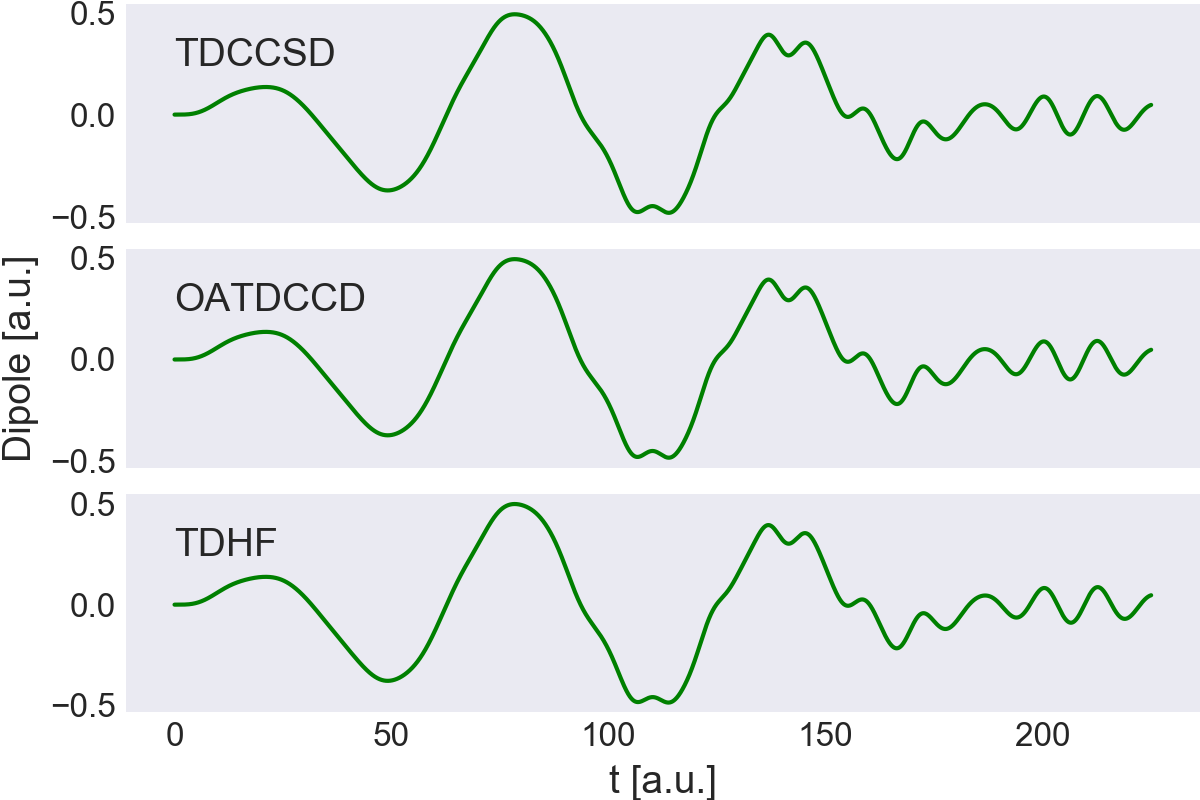
\includegraphics[width=0.75\textwidth]{results/figures/li_compare.png}
    \caption{Instantaneous dipole for $H_2$ in an oscillating electric field
        $E_\text{max} = 0.07 \text{ au}$ ($1.72\times10^14 \text{ W} \text{cm}^{-2}$)
        and $\omega=0.1 \text{ au}$ ($456\text{ nm}$) using a \lstinline{6-311++G(d,p)}
        basis set.
    }
    \label{fig:li_compare}
\end{figure}


\section{Ground State Probability in 1D Quantum Dot}

\citeauthor{Zanghellini04}\cite{Zanghellini04} calculate the time development of a 
one-dimensional quantum dot with two electrons using the multi-configurational 
time-dependent Hartree-Fock method (MCTDHF). This method yields excact results for 
a very large number of configurations, $\eta \to \infty$. This study would provide a 
proper benchmark for our implementation because the coupled cluster method with singles and 
doubles excitations (CCSD) is excact for $n=2$ particles. 
The harmonic oscillator potential applied in
their study had a frequency of $\Omega=0.25$, used a strong laser-like field with 
maximum intensity of $\vb{E} = 1$ and a laser frequency of $\omega = 8 \Omega = 2$.
The oscillating field is described much more simply than in
\citeauthor{li2005time}\cite{li2005time}, using a simple sine function,
\begin{equation}
    \vb{e}(t) = \vb{E}\sin(\omega t),
\end{equation}
where the envelope $\vb{E}$ does not vary in time.

\citeauthor{Zanghellini04}\cite{Zanghellini04} find that their multi-configurational time-dependent
Hartree-Fock scheme convergences as the number of configurations is 
$\eta \geq15$, up to the resulotion of their figures.
We are able to reproduce this result precisesly by employing the 
time-dependent coupled cluster method with singles and double excitations (TDCCSD).
We have used our own one-dimensional quantum dot class, \lstinline{ODQD}, with 
a harmonic potential and $l=20$ spin-orbitals
in the basis set for this simulation.

\begin{figure}
    \centering
    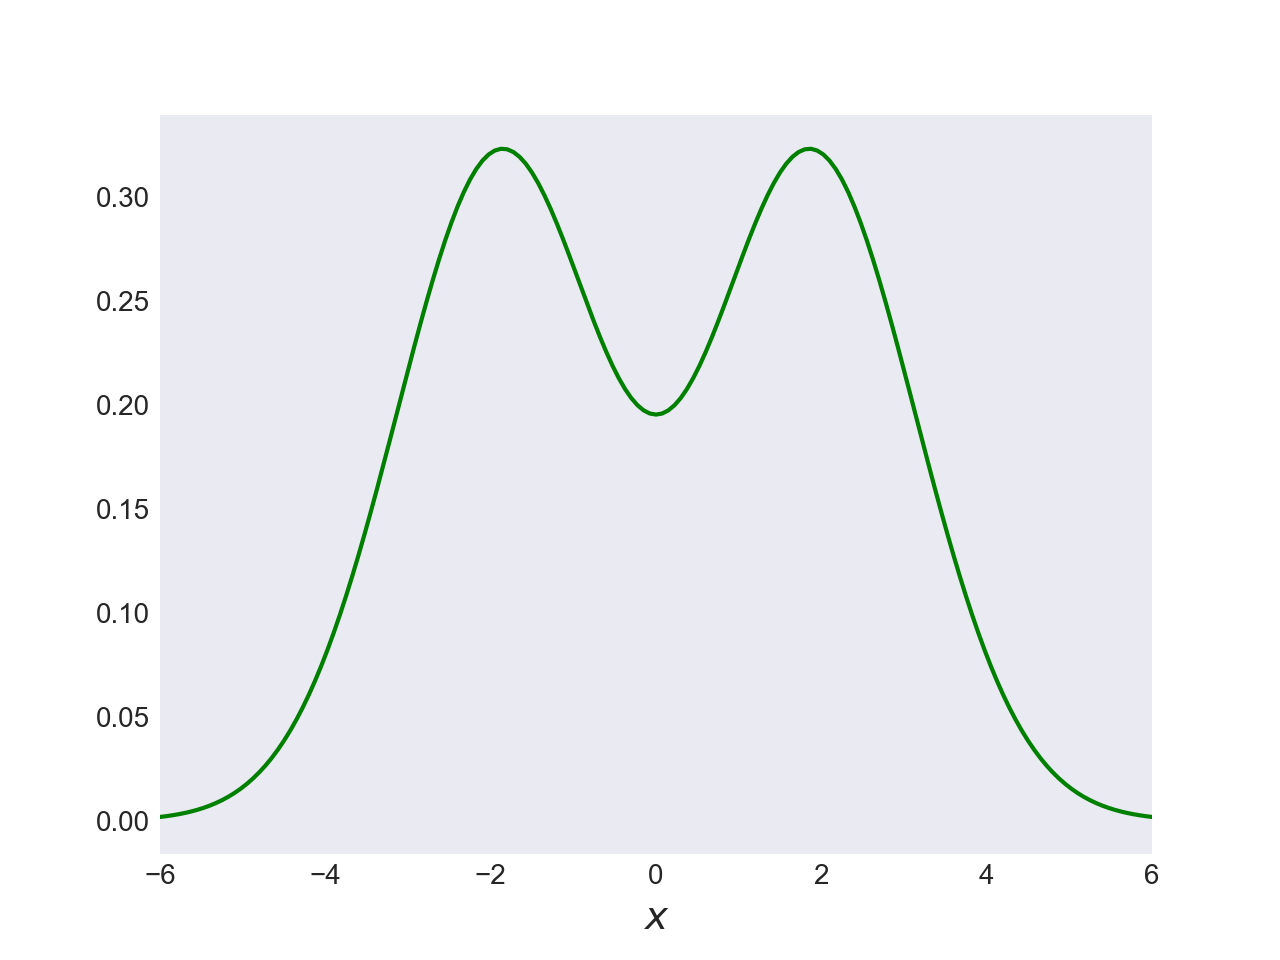
\includegraphics[width=0.75\textwidth]{results/figures/zanghellini_fig1.png}
    \caption{
        \label{fig:zanghellini_fig1}
        Electron density for the ground state wavefunction of a quantum dot with 
        $n=2$ eletrons and $l=20$ spin-orbitals in the basis set computed with
        CCSD. This plot 
        corresponds precisely with figure 1 in
        \citeauthor{Zanghellini04}\cite{Zanghellini04}.
    }
\end{figure}

\begin{figure}
    \centering
    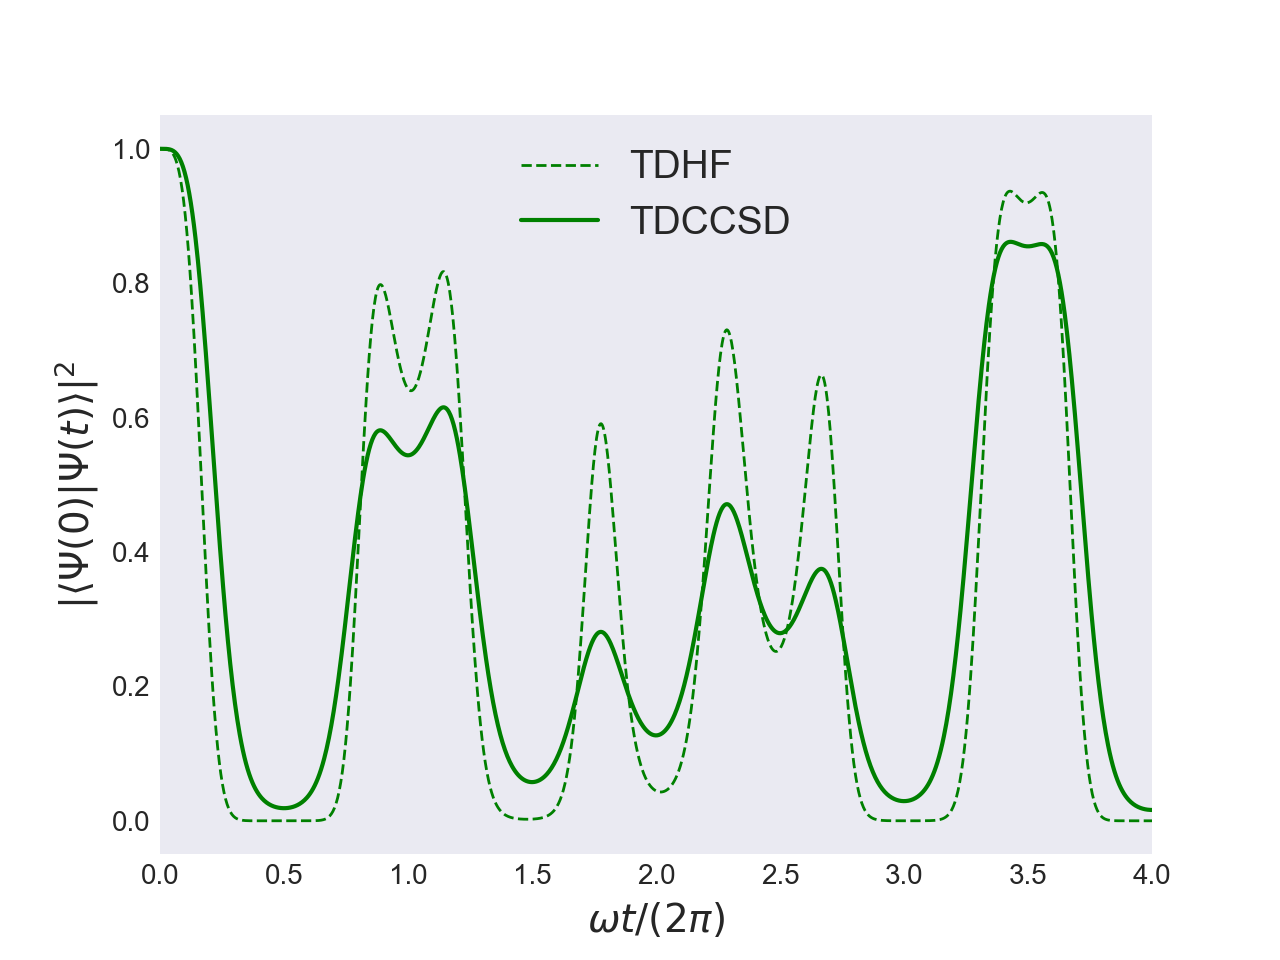
\includegraphics[width=0.75\textwidth]{results/figures/zanghellini_fig2.png}
    \caption{
        \label{fig:zanghellini_fig2}
        Probability of being in the ground state $|\braket{\Psi(0)}{\Psi(t)}|$
        using both TDHF and TDCCSD, for a one-dimensional quantum dot with $n=2$
        particles and $l=20$ spin-orbitals. This plot corresponds precisely with 
        figure 2 in \citeauthor{Zanghellini04}\cite{Zanghellini04}.
    }           
\end{figure}

In \autoref{fig:zanghellini_fig1} we see the ground state electron density for the 
ground state wavefunction computed with CCSD. \citeauthor{Zanghellini04} computed the electron
density for an increasing number of configurations $\eta$ using multi-configurational
time-dependent Hartree-Fock (MCTDHF). This figure matches the convergent electron density found by
\citeauthor{Zanghellini04} as $\eta \to \infty$, in figure 1 from their article. 

\autoref{fig:zanghellini_fig2} depicts the probability for the system being in the ground 
state as a function of time. Here we have included both a time-dependent Hartree-Fock
computation, corresponding to a multi-configurational time-dependent 
Hartree-Focke computation with $\eta=1$ configurations, and 
a time-depenedent coupled cluster computation with single and double excitations.
We see that our coupled cluster scheme corresponds to the multi-configurational Hartree-Fock 
scheme employed by \citeauthor{Zanghellini04} when $\eta\to\infty$, as
\autoref{fig:zanghellini_fig2} match figure 2 in
\citeauthor{Zanghellini04}\cite{Zanghellini04} precisely.


\section{Dipole Spectrum of Helium}

In their comparison study of symplectic and regular Runge-Kutta type integrators, 
\citeauthor{pedersen2019symplectic}\cite{pedersen2019symplectic} produce a dipole 
spectrum of helium. 

The basis set employed by \citeauthor{pedersen2019symplectic} is a cc-pVDZ 
basis set which we extract from \lstinline{Psi4},
\begin{python}
He = "
    He 0.0 0.0 0.0
    symmetry c1
"
options = {"basis": "cc-pvdz", "scf_type": "pk", "e_convergence": 1e-8}
system = construct_psi4_system(He, options)
\end{python}
The \lstinline{cc-pVDZ} basis set is a correlation consistent, polarised, valence-only 
basis set with double zeta-functions. For hydrogen this basis set amounts to five 
orbitals in total.

% \omega=2.8735643 \text{ au}
In their study \citeauthor{pedersen2019symplectic} use an oscillating field with 
frequency $\omega=2.8736 \text{ au}$ and maximum intensity
$\vb{E}_\text{max} = 10 \text{ au}$. This frequency corresponds to the lowest-lying 
electric-dipole allowed transition from the ground state of helium. The oscillating 
field can be described as 
\begin{equation}
    \vb{e}(t) = \vb{E}(t) \cos(\omega t),
\end{equation}
with a sinusoidal envelope
\begin{equation}
    \label{eq:pedersen_2019_envelope}
    \vb{E}(t) = \vb{E}_\text{max}\sin^2\left(\frac{\pi t}{t_d}\right) H(t_d - t),
\end{equation}
where $H$ is the Heaviside step function designed to return zero when the field 
has reached its designated halting time $t_d$. This envelope is similar in behaviour 
to the one in the study by \citeauthor{li2005time}\cite{li2005time} - it 
increaes gradually at first, and then gradually decreases. 

The oscillating field is only meant to ``disturb'' the ground state of the atom,
as it is quickly 
switched off at $t_d=5$. Then the system is allowed to propagate in time for 
a long period. In our reproduction of the system, we have let the system 
evolve for a total time $T=1500 \text{ au}$. For each time step we compute the 
dipole in the same direction as the polarisation of the oscillating field. The 
fourier transform of this signal will then yield the dipole spectrum of the 
atom. The time-development is performed with the orbital-adaptive time-dependent 
coupled cluster method with double excitations. The result from this simulation is 
depicted in \autoref{fig:helium_spectrum}, which is qualitatively equal to figure 
7 in \citeauthor{pedersen2019symplectic}\cite{pedersen2019symplectic}.

\begin{figure}
    \centering
    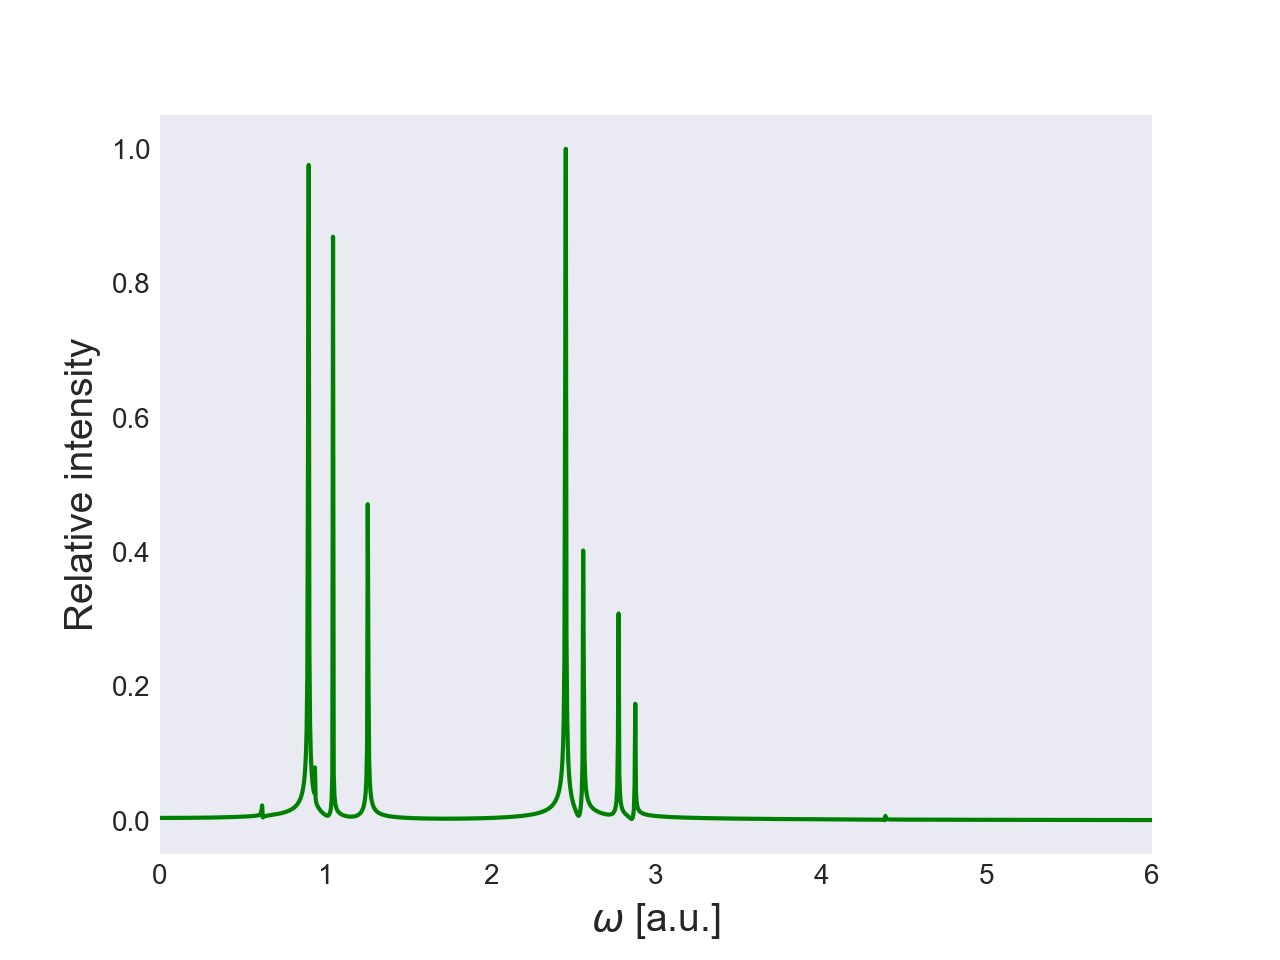
\includegraphics[width=0.75\textwidth]{results/figures/helium_spectrum.png} 
    \caption{Dipole spectrum of He at field strength $10\text{ au}$ using 
        OATDCCD and a \lstinline{cc-pVDZ} basis set.      
    }
    \label{fig:helium_spectrum}
\end{figure}


\section{Ionisation of 1D Beryllium}
\label{sec:miyagi_replication}

\citeauthor{miyagi2013time}\cite{miyagi2013time} implement the time-dependent 
restricted active space self consistent field singles (TD-RASSCF-S) method 
and compare it with time-dependent configuration interaction singles (TDCIS) and 
the multi-configurational time-dependent Hartree-Fock (MCTDHF) method. A simulation they 
perform in this study is the simulation of the ionisation of beryllium. This 
simulation is performed by applying an oscillating field defined by the following 
vector potential,
\begin{equation}
    \vb{A}(t) = \frac{\vb{E}_\text{max}}{\omega}\sin\left(\frac{\pi t}{T} \right),
\end{equation}
giving the following field
\begin{equation}
    \vb{e}(t) = - \vb{E}_\text{max}\sin\left(\frac{\pi t}{T} \right)
    \left[
        \frac{2\pi}{T\omega} \cos\left(\frac{\pi t}{T} \right) \sin\left(\omega t \right)
        + \sin\left(\frac{\pi t}{T} \right) \cos(\omega t)
    \right].
\end{equation}
We reproduce the one-dimensional beryllium model with our \lstinline{AtomicPotential}
class, which can be passed as a potential to the \lstinline{ODQD}
(one-dimensional quantum dot) class when setting up the system,
\begin{python}
Z = 4; n = 4; l = 40; c = 1; a = 1; alpha = 1;
potential = AtomicPotential(Z, c)
odbe = ODQD(n, l, grid_length, num_grid_points, a, alpha)
odbe.setup_system(potential=potential)
\end{python}
where \lstinline{Z} are the number of protons, \lstinline{n} is the number of electrons,
\lstinline{l} is the number of spinorbitals, \lstinline{c} is the position of the nucleus,
\lstinline{a} is the Coulomb screening parameter and \lstinline{alpha} is the strength of the 
Coulomb interaction. We pick a wide grid of $300 \text{ au}$, with $5001$ points, and 
a time step size of $\Delta t=0.01$. The maximum field strength is set to
$\vb{E}_\text{max} = 0.0755 \text{ au}$ and the frequency of the laser field is set to
$\omega = 0.057 \text{ au}$. This corresponds to a peak intensity of 
$2.0 \times 10^{14} \text{ W cm}^{-2}$ and a laser wavelength of $800 \text{ nm}$.

The idea behind the simulation is to compute the particle density over time, and see if 
there is more than significantly high probability to see an electron very far away from the 
nucleus. The total time of the simulation is $T=331 \text{ au}$, and the particle density 
$\rho(x, t)$ is computed at the very beginning of the simulation, halfway through 
and at the end of the simulation. We do this both with our time-dependent coupled 
cluster singles doubles (TDCCSD) method with static orbitials and 
the orbital-adaptive time-dependent 
coupled cluster doubles method (OATDCCD). 
The results of the simulations are shown in 
\autoref{fig:miyagi_fig4}.

\begin{figure}
    \centering
    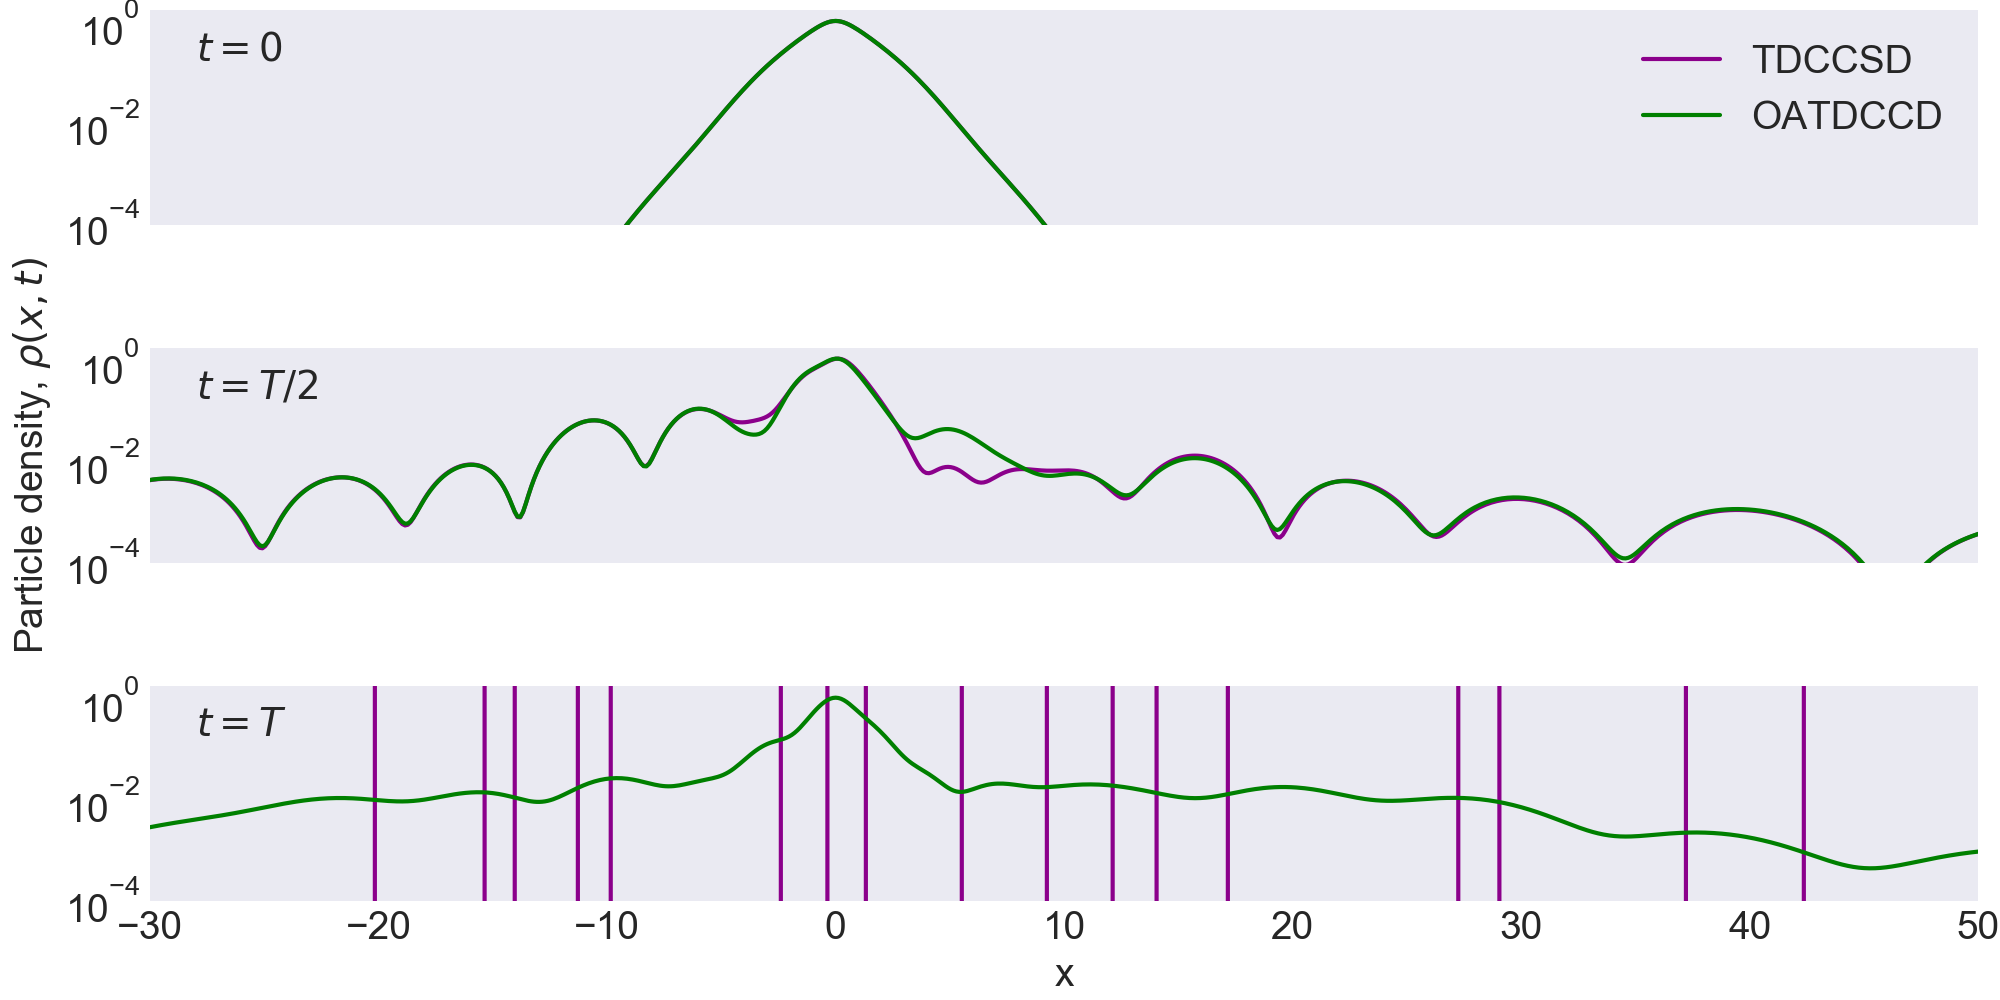
\includegraphics[width=\textwidth]{results/figures/miyagi/fig4_miqyagi.png} 
    \caption{Snapshots of the electron density $\rho(x, t)$ in the 1D beryllium atom 
        at $t=0$, $t=T/2$ and $T$, computed with TDCCSD and OATDCCD. 
    }
    \label{fig:miyagi_fig4}
\end{figure}

In the top subfigure in \autoref{fig:miyagi_fig4} we see the electron density before 
the system is developed in time, and the two methods are in good agreement. In 
the middle subfigure the simulation is halfway through its course and the two methods
both appear to show the same effects, but with 
slight discrepancies. In the bottom subfigure, we see that the OATDCCD method is doing
fine, but the TDCCSD is absolutely non-sensible. We can conclude that the propagating 
obitals in time enables us to get the same qualitative result as \citeauthor{miyagi2013time}
in figure 4 from their study. Keeping the orbitals static as in the TDCCSD method makes 
us unable to model the same behaviour. We will delve a bit deeper to try to shed 
some light on why the TDCCSD method fails.

\begin{figure}
    \centering
    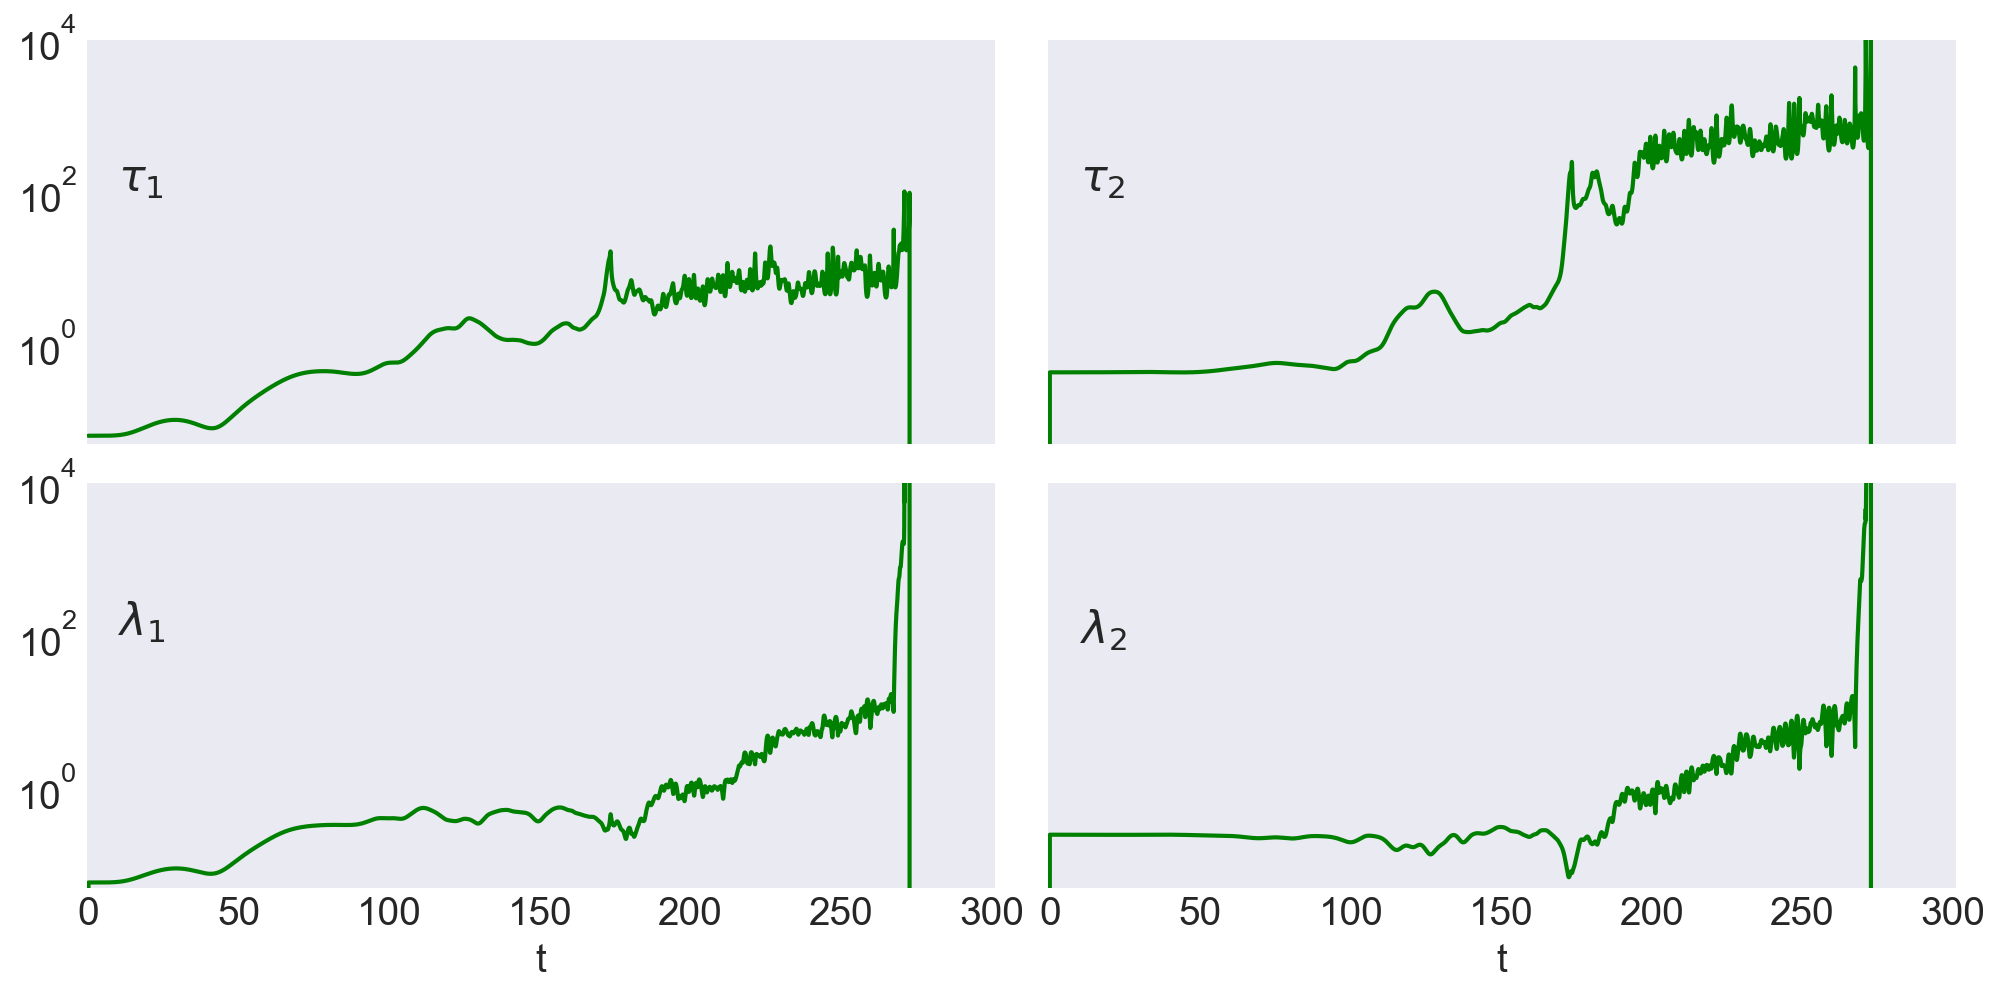
\includegraphics[width=\textwidth]{results/figures/miyagi/amplitude_norm_tdccsd.png} 
    \caption{Norm of the amplitudes over time in the 1D beryllium atom, computed 
        with TDCCSD. We see unreasonably high amplitude norms.
    }
    \label{fig:miyagi_tddccsd_amplitude}
\end{figure}

If we compute the norm of the amplitudes over the course of the simulation for 
the time-dependent coupled cluster singles doubles (TDCCSD) method, we get the 
result shown in \autoref{fig:miyagi_tddccsd_amplitude}. In essence, the amplitudes 
in any coupled cluster computation provides a linear combination of orbitals 
from the reference state $\ket{\Phi_0}$, in order to provide the best representation of the 
exact state $\ket{\Psi}$. For this reason one would not expect the norm of the 
amplitudes to be realtively low for an exact that is close to the reference state.
We encounter problems with the static orbitals because we are dealing with a system that
moves very far 
from its inital state. In \autoref{fig:miyagi_tddccsd_amplitude} we see
that the amplitudes stay within a reasonable magnitude for up to about halfway through 
the simulation, after which we see the method is struggling greatly to 
represent the current state with the basis it has been given. In figure 
\autoref{fig:miyagi_tdccsd_overlap}, a plot of the 
overlap of the current, time-dependent state with the initial ground state
helps to underline this point. The inset figure in \autoref{fig:miyagi_tdccsd_overlap}
shows the area of the figure with the highest value for the overlap, at a larger scale.
We see that the ground state probability reaches values of more than $300$, which is 
most definitely unreasonable, because a probability like this should always be between 
$0$ and $1$.

\begin{figure}
    \centering
    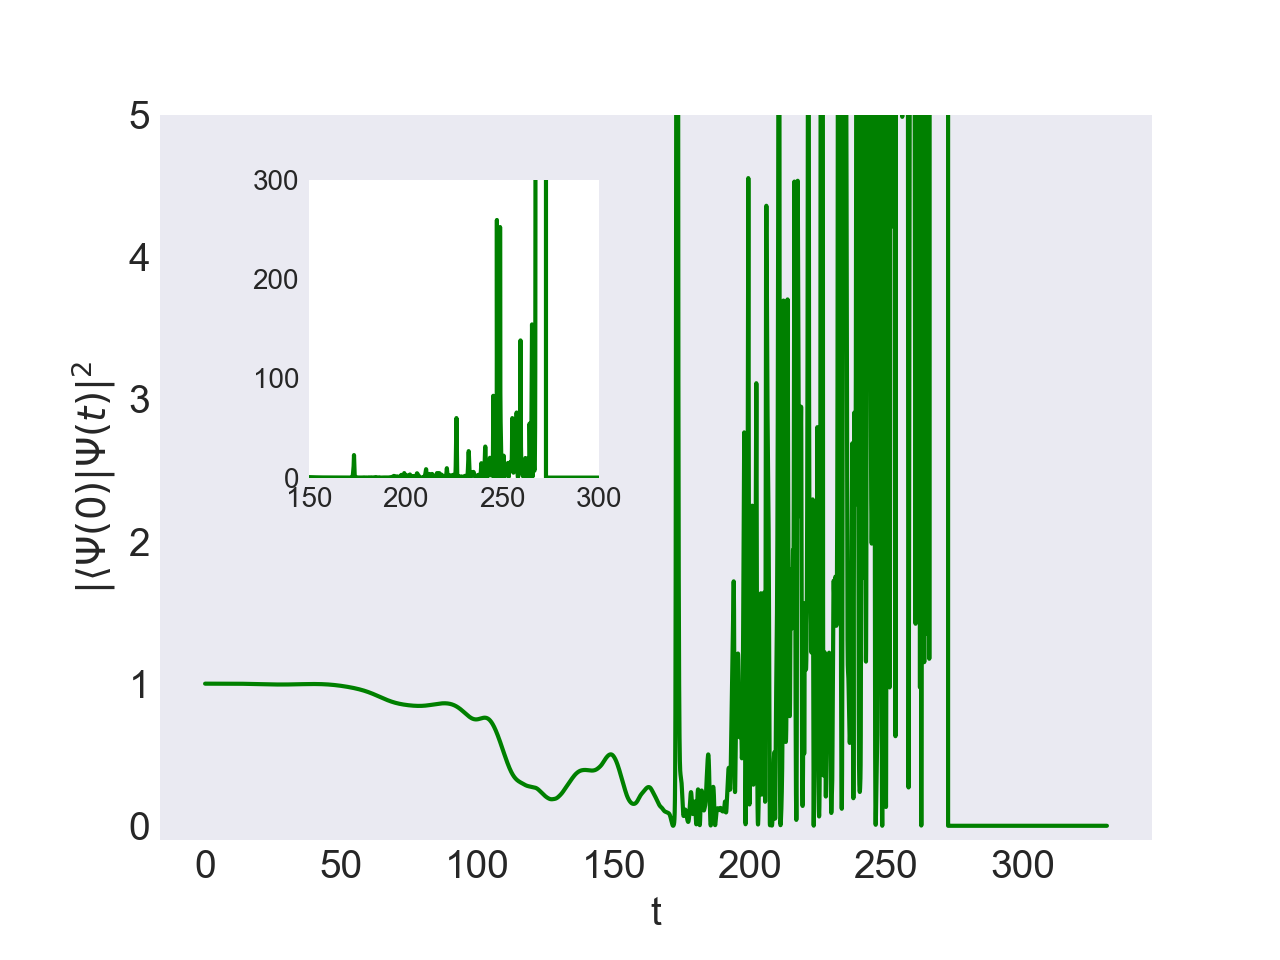
\includegraphics[width=0.75\textwidth]{results/figures/miyagi/overlap_tdccsd.png}
    \caption{Probability of being in the ground state over time 
        $|\braket{\Psi(0)}{\Psi(t)}|$ in the 1D beryllium atom, computed with TDCCSD. 
        We see impossibly unreasonable probabilities.
    }
    \label{fig:miyagi_tdccsd_overlap}
\end{figure}

It is difficult to draw a clear conclusion as to when the time-dependent coupled cluster 
method with static orbitals breaks down and is unfeasible for use. However, we can 
draw some broader, qualitative strokes towards a diagnosis of the problem. Any coupled 
cluster method is supposed to provide the best representation of a system's exact 
wavefunction by picking fitting parts of the basis set contained in the reference 
state for that system. If the exact wavefunction exists in a very different basis 
space than the reference state, it stands to reason that it is very difficult, if 
not impossible to find a mapping between the two. This problem stems from the foundations 
of the approximative nature of the coupled cluster method as it has a truncated basis set. 

\citeauthor{pedersen2019symplectic}\cite{pedersen2019symplectic} provide a similar 
deduction, highlighting there what appears to be a system-dependent upper limit for 
the strength of the external field. They underline the improvement in the computations 
by using a symplectic integrator instead of a standard fourth-order Runge-Kutta method.
We use the exact same integrator as the one \citeauthor{pedersen2019symplectic} outline.
\citeauthor{pedersen2019symplectic} argue that a large amplitude norm should make one 
question the validity of the result. It is difficult to gauge what constitutes a ``large''
amplitude norm, however.

Lastly with regards to the ionisation study from \citeauthor{miyagi2013time}\cite{miyagi2013time},
we would like to emphasise how well the orbital-adaptive time-dependent coupled cluster 
doubles (OATDCCD) method performs. OATDCCD manages to replicate the desired results 
to a significant degree, giving relatively high values for the entire grid 
of the particle density represented in \autoref{fig:miyagi_tdccsd_overlap}. This is 
normally interpreted as a free praticle because one would expect the wavefunction of 
a free particle to spread out in space as time progresses.
        \chapter{Quantum Dots}

Here we present results related to time-dependent simulations of parabolic quantum
wells. We have simulated the behaviour of such quantum dots in both one- and two 
dimensions, producing time dependent energies and ground state probabilities over
time as the system is under the influence of oscillating fields. We also present 
dipole spectra of the one- and two-dimensional quantum dot as well as the 
two-dimensional double dot and a two-dimensional double dot under the influence of
a homogenous, static magnetic field. We find that the \emph{harmonic potential theorem}
holds for all simulations.

The \emph{harmonic potential theorem}\cite{kohn1961cyclotron}
states that electrons trapped in a parabolic quantum well shows behaviour as if it 
was one large quantum oscillator, instead of consisting of many smaller parts. This 
includes exhibiting only one frequency in the dipole spectrum of the system. If one 
were to compute the Fourier transform of the dipole of an $n$-electron quantum dot with 
parabolic potential the result would be one line in the spectrum corresponding to the
oscillator frequency of the spectrum. This means that in the dipole approximations,
 we can not detect many-body effects in a harmonic quantum dot with infra-red light.

An extension of the theorem to systems under the influence 
of a magntic field\cite{brey1989optical}. State that one would expect to see a shift,
both up and down, creating two frequencies $\Omega_+$ and $\Omega_-$ in the dipole 
spectrum. The resulting dipole spectrum would show two frequencies with a difference 
equalling the Larmor frequency $\omega_c = \Omega_+ - \Omega_-$.

\section{Harmonic Oscillators in One Dimension}

For the one-dimensional quantum dot with a harmonic potential we simulate a laser by 
adding an oscillating 
field with a sinusoidal envelope, similar to the one in
\citeauthor{pedersen2019symplectic}\cite{pedersen2019symplectic},
\begin{equation}
    \label{eq:results_1d_field}
    \vb{e}(t) = \vb{E}_\text{max}\sin^2\left(\frac{t\pi}{T}\right)\cos(\omega t).
\end{equation}
We set the period of the envelope equal to the duration of the entire simulation,
$T=20$, so that we have a field that at first will gradually increase, then decrease.
The oscillator frequency for all simulations are set to $\Omega=1$, and at first we 
set the frequency of the oscillating field to twice this, $\omega = 2$. We do this 
to make sure that we are far from the resonant frequency of the system, and we pick 
relatively high laser frequency in order to enforce a more dynamic system. We use the 
more standard time-dependent coupled cluster singles doubles (TDCCSD) method, for 
these simulations, with the symplectic Gaussian integrator and a time step of
$/Deltat=0.01$.
The simulations are performed for an increasing number of electrons
$n = \{2,4,6,8,10,12\}$. We have computed the energy and the time-dependent overlap,
i.e. the time-dependent probability of being in the ground state, for each simulation.
We repeat the simulations for a wide range of different number of spin-orbitals,
in order to find convergent properties of the simulations as the number of spin-orbitals increase.

\begin{figure}[ht]
    \centering
    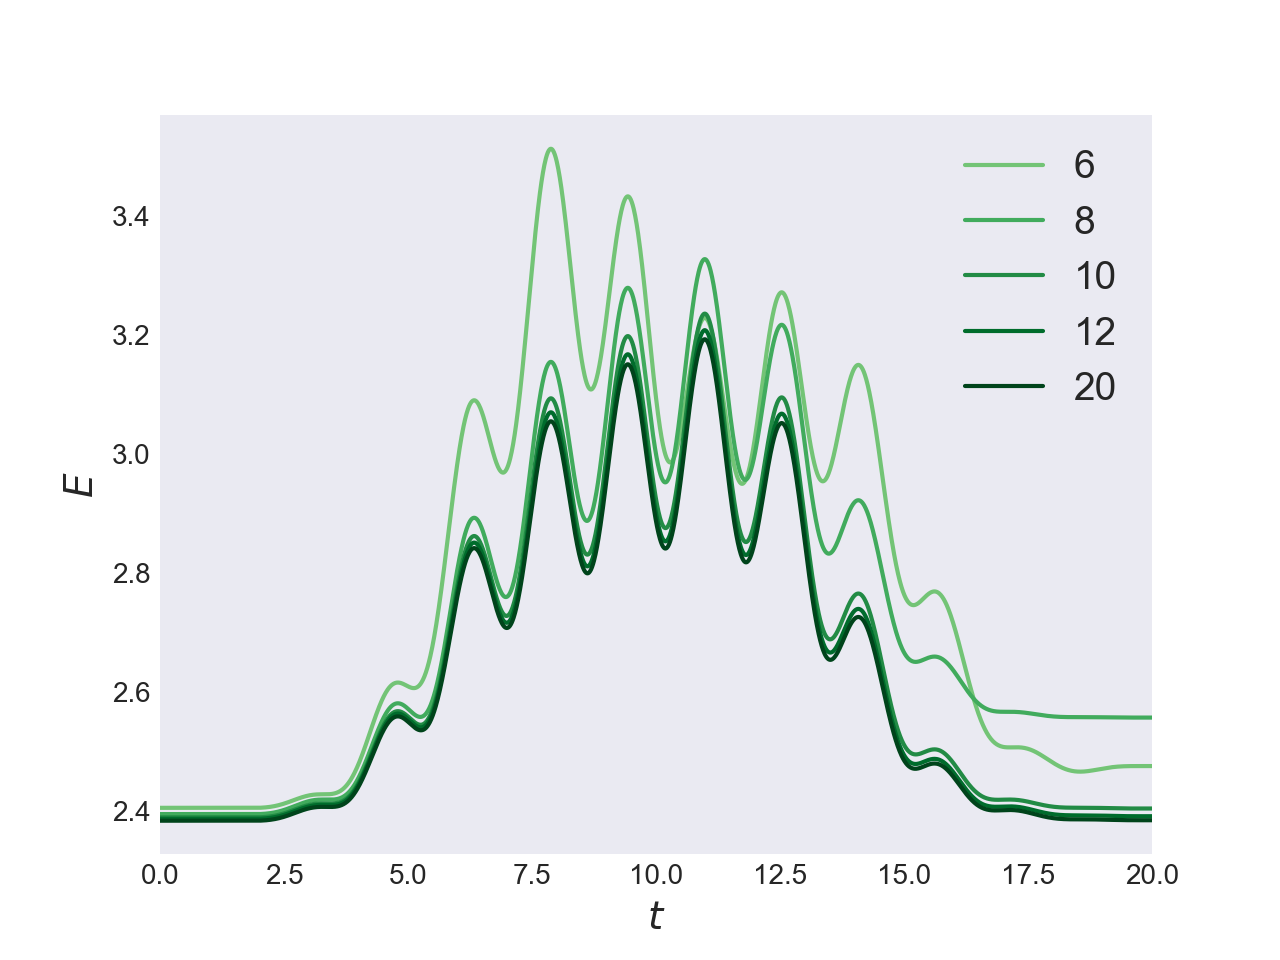
\includegraphics[width=0.75\textwidth]{results/figures/1D/n=2energy.png} 
    \caption{Time-dependent energy of a one-dimensional harmonic oscialltor 
        with $n=2$ electrons
        under the influence of a laser field for different number of spinorbitals
        $l\in\{6,8,10,12,20\}$.
    }
    \label{fig:1d_n2_E}
\end{figure}

First we study the time-dependent energy of a quantum dot acted upon by an oscillating 
field. The result for $n=2$ electrons is shown in \autoref{fig:1d_n2_E}. We have 
produced comparative results for other number of particles $n=\{4,6,8,10,12\}$,
which can be found in \autoref{app:1d_qd}. We see an apparent convergence in the 
time-dependent energy as we increase the number of spin-orbitals in the basis set.
For larger systems with more electrons it reasonably becomes necessary to also increase
the size of the basis set. As is the tendency with ground state coupled cluster computations
for quantum dots\cite{jorgensen2011many,lohne2010coupled}, the time dependent energy 
of a quantum dot is decreasing until convergence for increasing basis set size.

We see the same general convergent tendency when computing the time-dependent ground 
state probability $|\braket{\Psi(0)}{\Psi(t)}|^2$, shown in \autoref{fig:1d_n2_overlap} for $n=2$ electrons. We see that 
for lower number of spin-orbitals, the computation of overlap with 
the ground state tends to return a lower value than for a higher number of spin-orbitals.

\begin{figure}
    \centering
    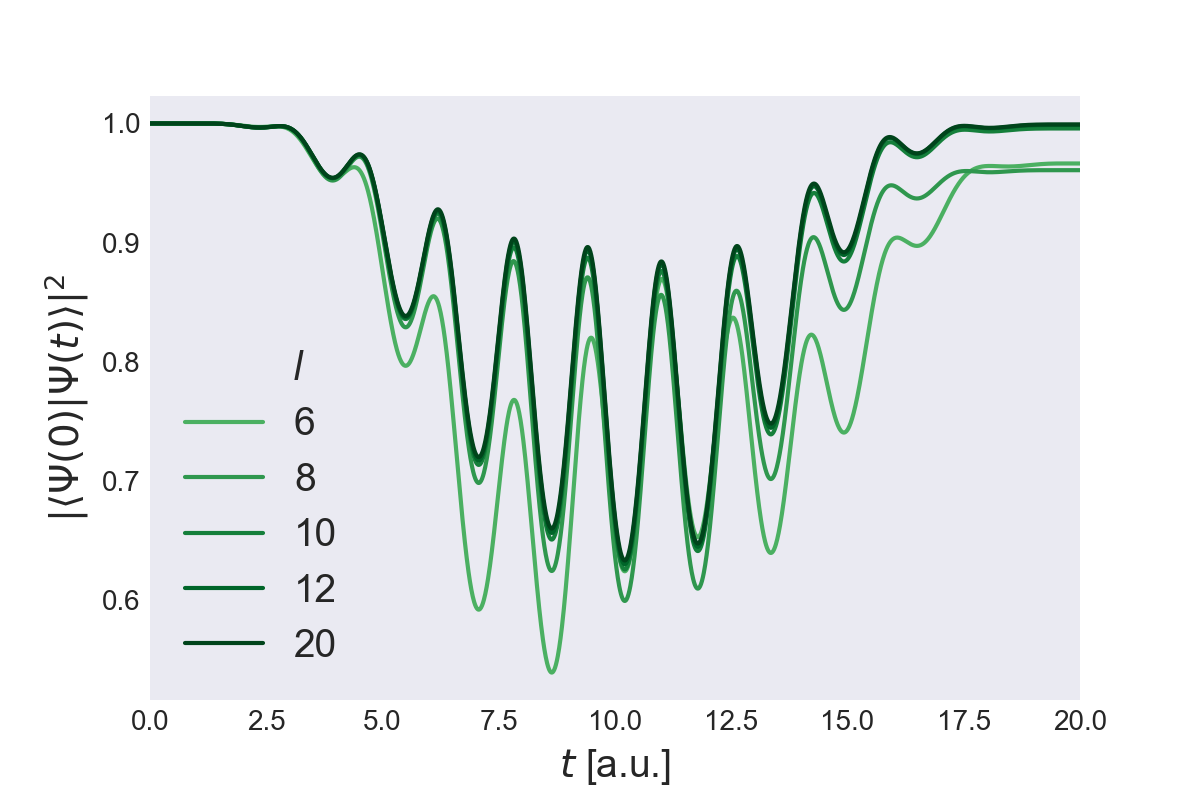
\includegraphics[width=0.75\textwidth]{results/figures/1D/n=2overlap.png} 
    \caption{Probability of being in the ground state $|\braket*{\Psi(0)}{\Psi(t)}|^2$
        for a one-dimensional quantum dot with $n=2$ electrons under 
        the influence of a laser field for different number of spinorbitals 
        $l\in\{6,8,10,12,20\}$.
    }
    \label{fig:1d_n2_overlap}
\end{figure}

Since the ground state probability is a number between zero and one, the results for systems 
of different number of electrons are comparable. We have produced such a comparison in 
\autoref{fig:1d_ground_state_prob_compare}. In this figure we have chosen the number of
spin-orbitals that would produce a convergent plot for the given system size. The general 
tendency is that a system with more electrons is less likely to be in the ground state 
over time, than a system with less electrons.

\begin{figure}
    \centering
    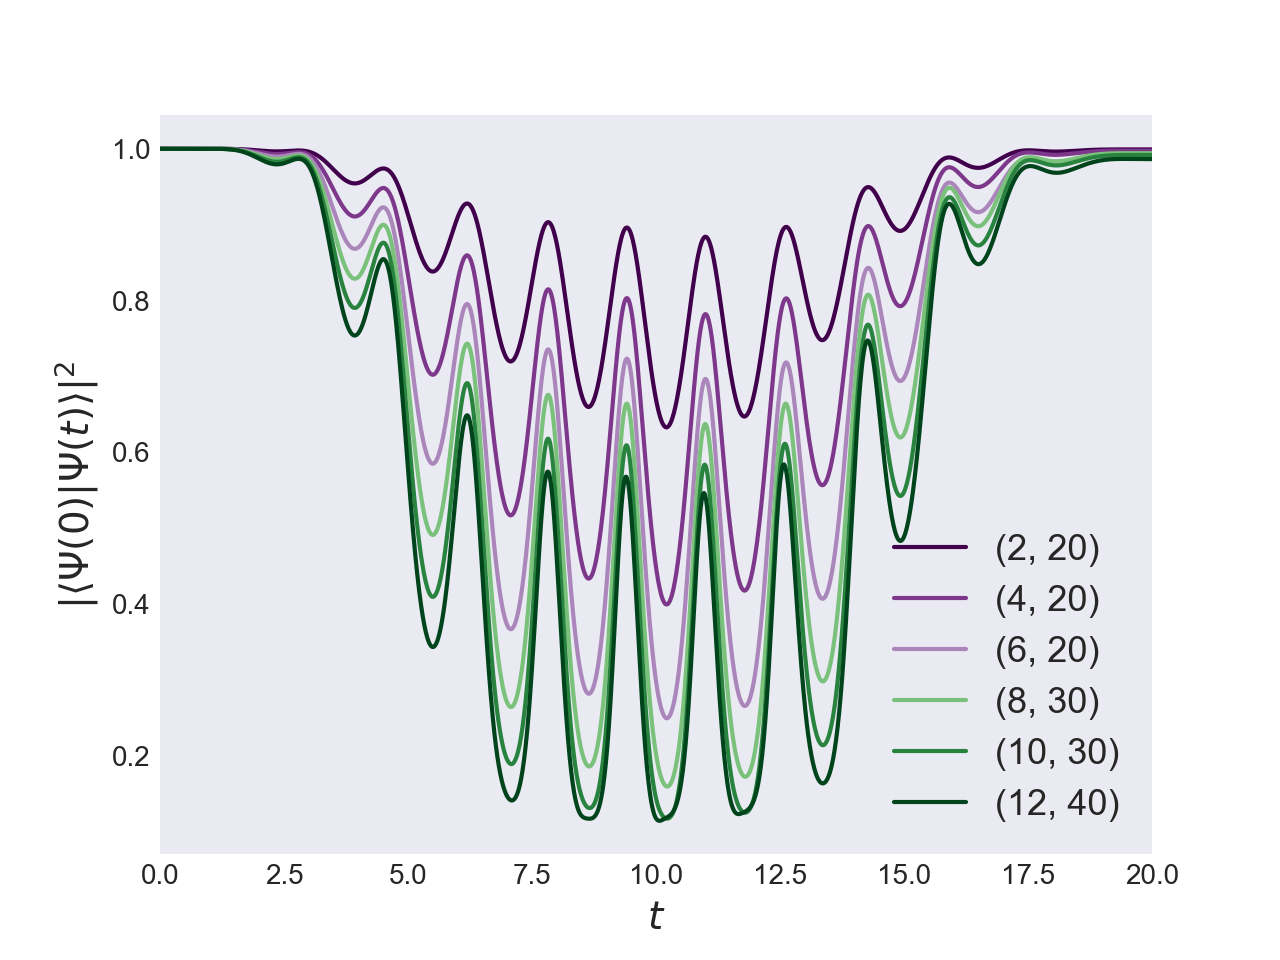
\includegraphics[width=0.75\textwidth]{results/figures/1D/n_compare_overlap.png} 
    \caption{Probability of being in the ground state for $|\braket*{\Psi(0)}{\Psi(t)}|^2$
        for a one-dimensional quantum dot for different number of electrons 
        $n = \{2,4,6,8,10,12\}$, with accompanying spin-orbitals $l=\{20,20,20,30,30,40\}$.
    }
    \label{fig:1d_ground_state_prob_compare}
\end{figure}

\subsection{Dipole spectrum}

We now turn to a somewhat different kind of simulation. We keep the 
base system the same, a one-dimensional quantum dot with harmonic potential and oscillator 
frequency $\Omega=1$. We also apply an external oscillating field like in
\autoref{eq:results_1d_field}, which will this time be resonant with the frequency of the 
oscillator $\omega=\Omega=1$, to ensure population of excited states. In this simuation 
we set the field to zero at $T_d = 5 \text{ au}$, by the use of a Heaviside function in a 
similar manner as \citeauthor{pedersen2019symplectic}\cite{pedersen2019symplectic}
in \autoref{eq:pedersen_2019_envelope}. After the field has been switched off we propagate 
the system in time for a total of $T = 500 \text{ au}$ with a time step $\Delta t=0.01$.
The same procedure is repeated for systems with $n=\{2,4,6,8,10,12\}$ electrons with 
respective number of spin-orbitals $l=\{20,20,20,30,30,40\}$. These system and basis 
sizes correspond to the ones used in \autoref{fig:1d_ground_state_prob_compare}.
For each time step we collect the dipole, i.e. $\ev{\hat{x}(t)} = \tr{\rho(t) x}$, and compute the 
Fourier transform of the entire collected array. The results are presented in 
\autoref{fig:1d_dipole_spectra}.

\begin{figure}
    \centering
    \makebox[\textwidth][c]{
    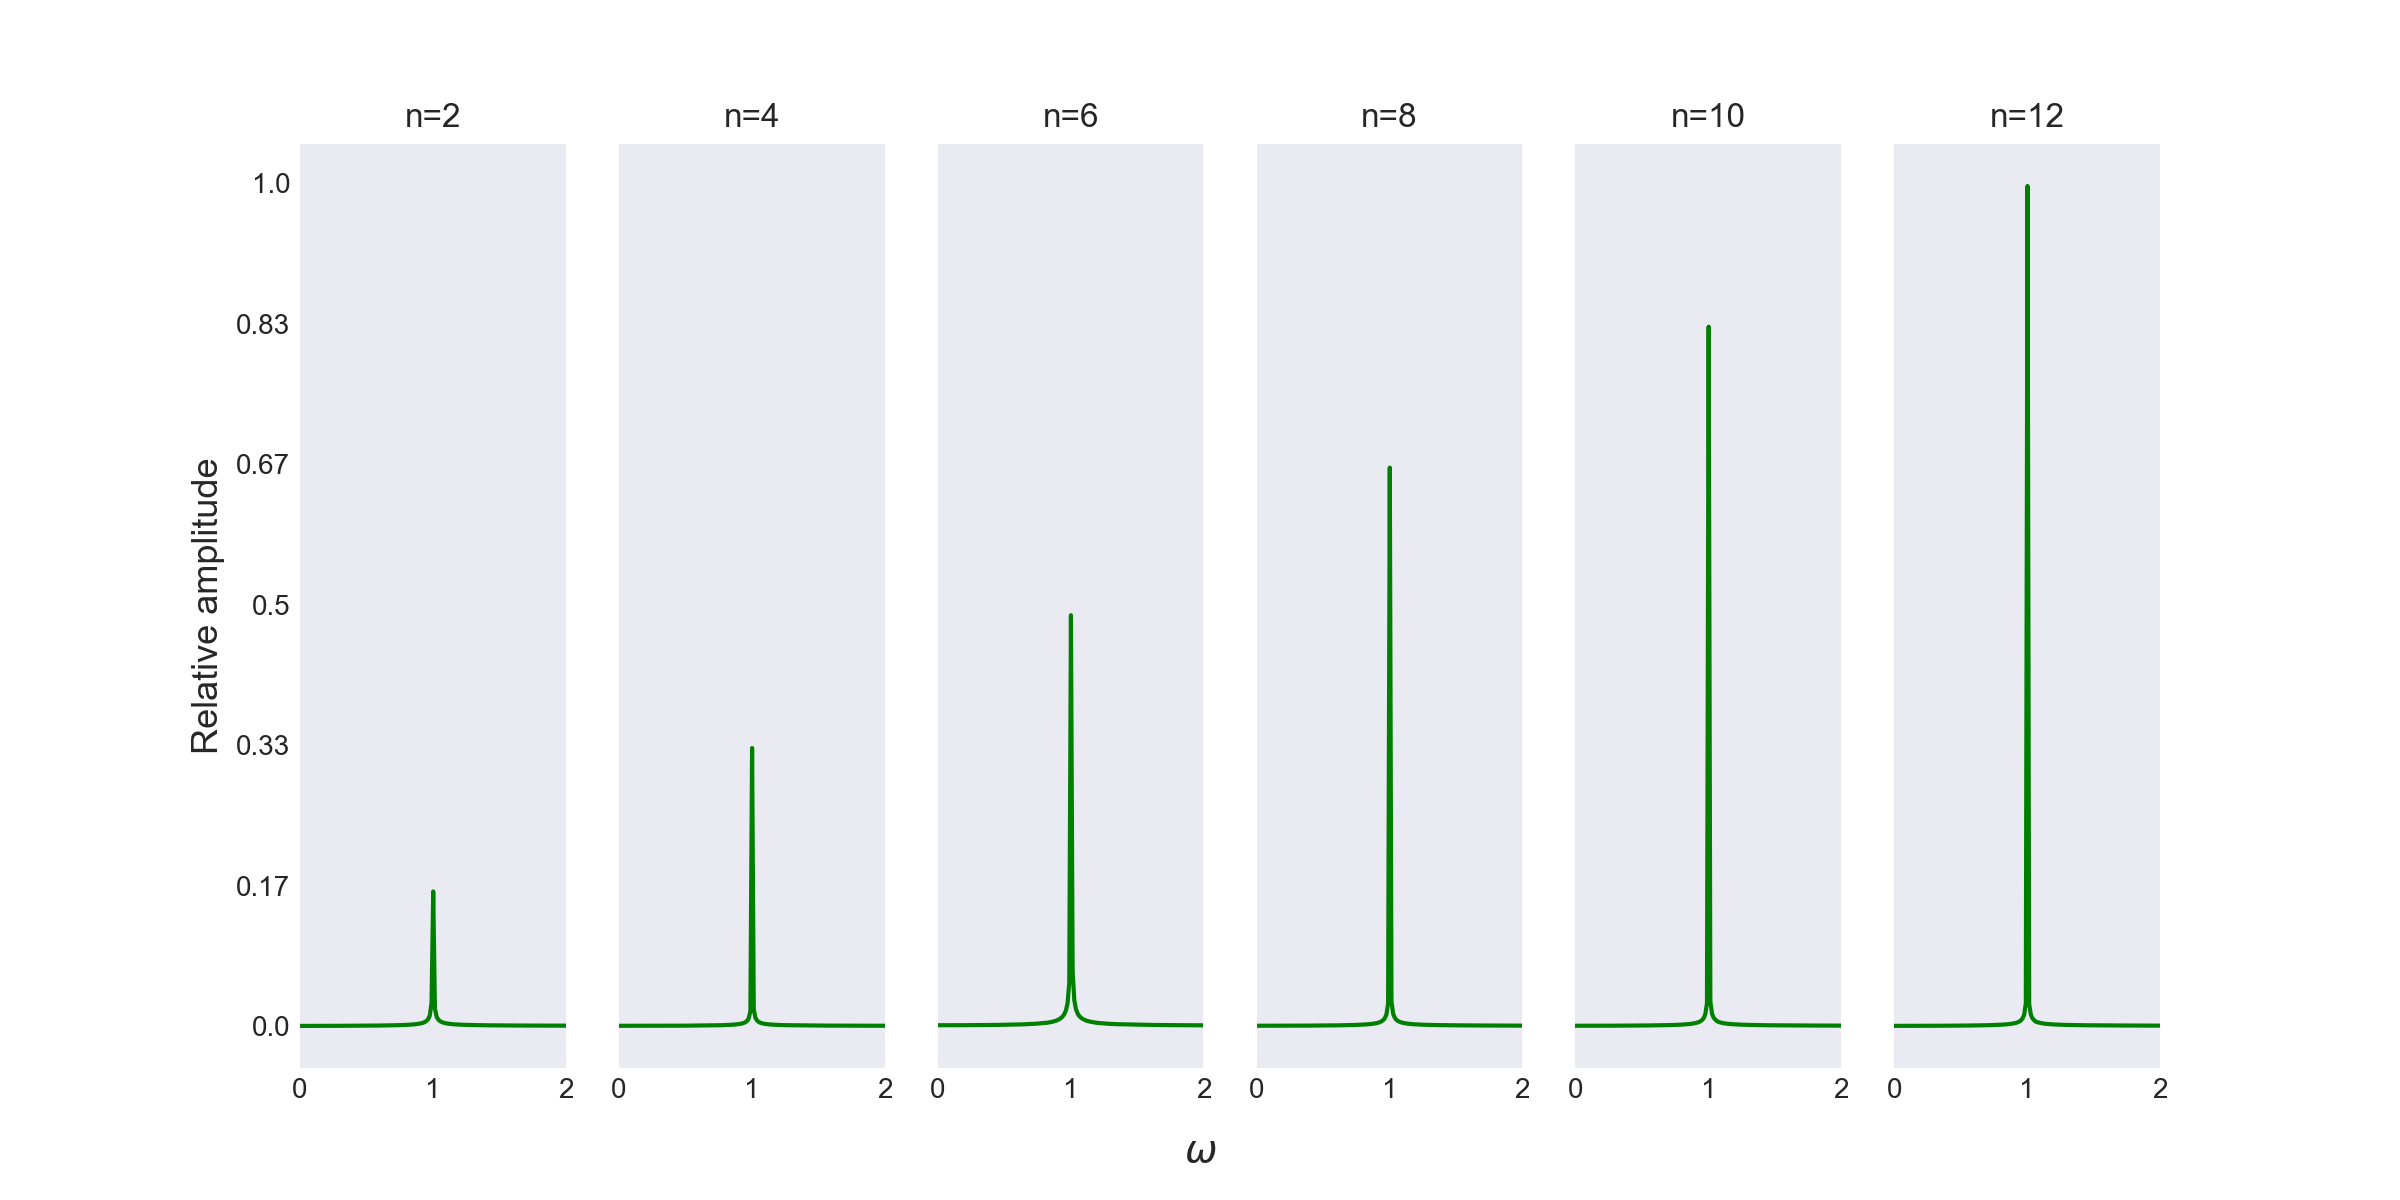
\includegraphics[width=1.4\textwidth]{results/figures/1D/1d_spectrum.png} 
    }
    \caption{Fourier transform of expected value of dipole moment for 
        a one-dimensional quantum dot with different number of electrons
        $n=\{2,4,6,8,10\}$ with respective number of spin-orbitals 
        $l=\{20,20,20,30,30,40\}$.
    }
    \label{fig:1d_dipole_spectra}
\end{figure}

We see that the result is in accordance with the harmonic potential theorem, as the 
simulations have produced dipole spectra that show only one line corresponding to the 
frequency of the confining potential. Morover, we see that the relative intensity of 
the spectra increases with the number of particles.

\subsection{Resonance Sensitivity}

In order to test the response of a quantum dot as the frequency of the oscillating 
field apporaches the oscillator frequency, we have run simulations for a selection 
of laser frequencies $\omega$ with the field described by \autoref{eq:results_1d_field}.
We chose frequencies $\omega\in\{1.0, 1.25, 1.5, 1.75, 2.0\}$ and set the 
oscillator freqcuencies of the quantum dot systems to $\Omega=1$. The laser pulse 
had a set period of $T_l=20 \text{ au}$, starting from $t=0$, while time-development 
of the system was allowed to continue to $T=30 \text{ au}$. The results of these 
simulations are shown for $n=2$ particles in \autoref{fig:n2_1d_resonance_energy}
and \autoref{fig:n2_1d_resonance_overlap}, which show the time-dependent energy 
and the time-dependendent ground state probabilities
$|\braket{\Psi(0)}{\Psi(t)}|^2$ respectively.

\begin{figure}
    \centering
    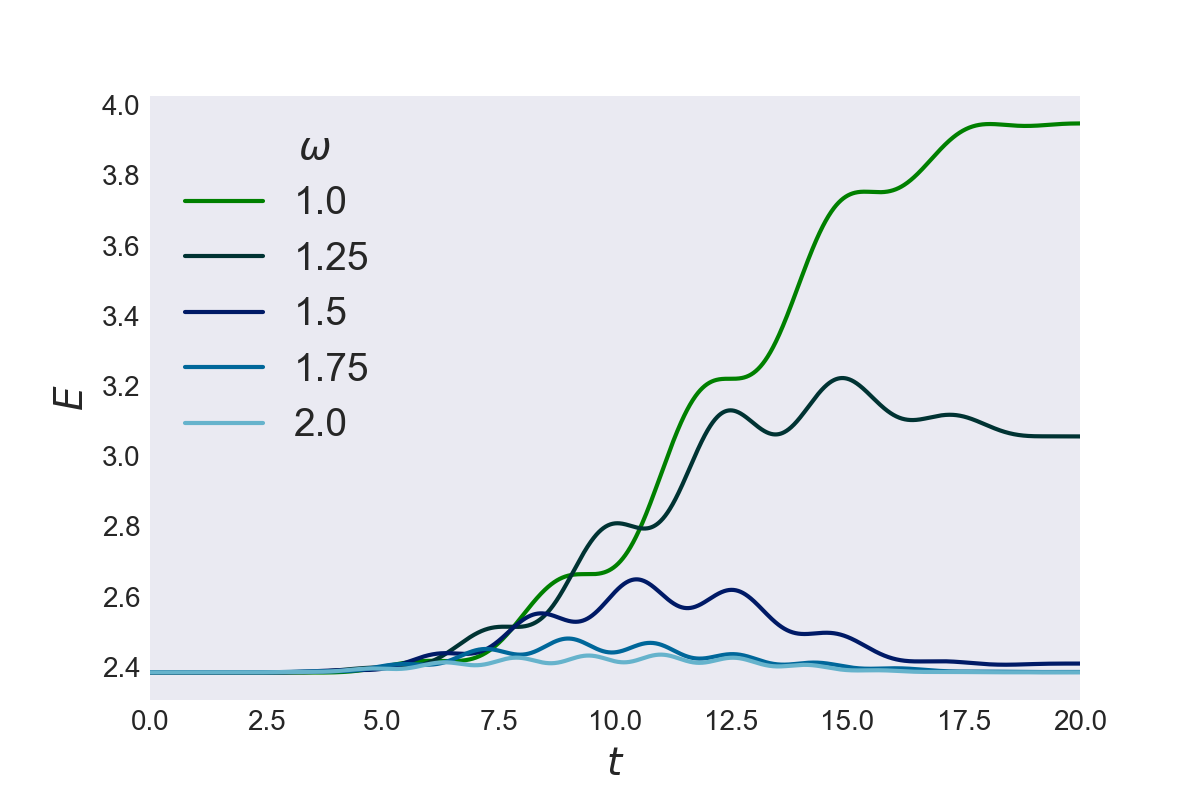
\includegraphics[width=0.75\textwidth]{results/figures/1D/n2_resonance_energy.png} 
    \caption{Time-dependent energy of a one-dimensional quantum dot with
        oscillator frequency $\Omega=1$ and $n=2$ electrons.
        The quantum dot is influenced by an oscillating field of different 
        frequencies $\omega\in\{1.0, 1.25, 1.5, 1.75, 2.0\}$ with a maximum 
        intensity of $\vb{E}_\text{max} = 0.25$.
    }
    \label{fig:n2_1d_resonance_energy}
\end{figure}

\begin{figure}
    \centering
    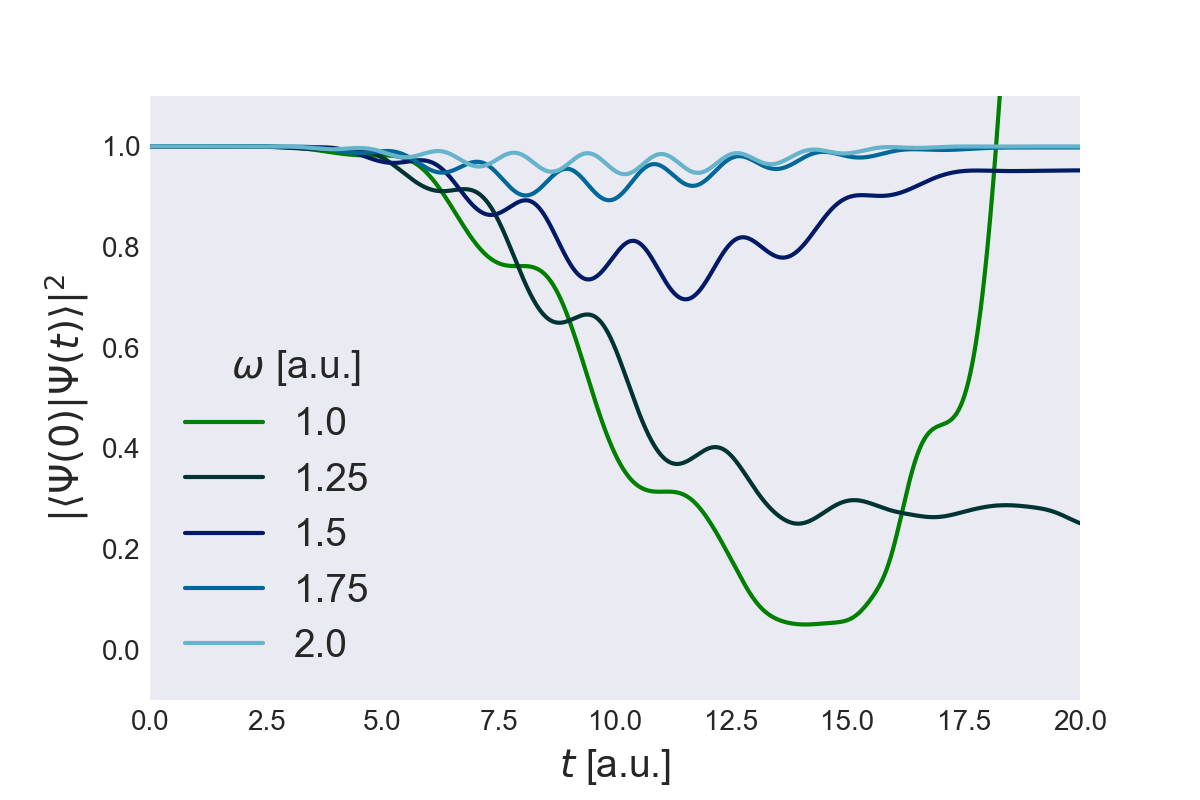
\includegraphics[width=0.75\textwidth]{results/figures/1D/n2_resonance_overlap.png} 
    \caption{Time-dependendent ground state probability $|\braket{\Psi(0)}{\Psi(t)}|^2$
        of a one-dimensional quantum dot with
        oscillator frequency $\Omega=1$ and $n=2$ electrons.
        The quantum dot is influenced by an oscillating field of different 
        frequencies $\omega\in\{1.0, 1.25, 1.5, 1.75, 2.0\}$ with a maximum 
        intensity of $\vb{E}_\text{max} = 0.25$.
    }
    \label{fig:n2_1d_resonance_overlap}
\end{figure}

The results are as expected, but interesting nonetheless. We see that the quantum dots 
behave very much as a classical driven harmonic oscillator. If the frequency of the driving
force, in this case the oscillating field, is far from the resonant frequency of the 
system the system falls back to the inital position after the force subsides. Only when we 
get closer to the resonant system do we see an excitation in energy of the system as 
a whole after the laser field is switched off (\autoref{fig:n2_1d_resonance_energy}).
In the case for the exact resonant frequency,
such that $\omega=\Omega$, we se that the energy of the system is increased even at the very 
end of the simulation, when the amplitude of the oscillating field is miniscule.
The same effects are apparent when studying the overlap of the time-developed system 
with the initial ground state in \autoref{fig:n2_1d_resonance_overlap}. Closer to the
resonant frequency we see a much lower probability of being in the ground state. For 
frequencies far away from the resonant frequency we see that the system falls back to 
the exact ground state or a state close to the ground state.

We have run similar simulations to the one described above, in order to study the 
resonant properties of a quantum dot, for $n=4,6,8,10$ electrons in a one-dimensional 
quantum dots. Figures with the results from these simulations can be found in 
\autoref{app:1d_qd}. In the ground state probability plots for these simulations, 
one would notice non-sensible probabiliy values $|\braket{\Psi(0)}{\Psi(t)}|^2 > 1$.
This is an issue we have adressed in the following sections, when reviewing the results 
of the two-dimensional quantum dot results.


\section{Two-dimensional Quantum Dot}

The two-dimensional quantum dot arguably paints a somewhat more interesting picture 
than the one-dimensional quantum dot, as we shall see. We construct several 
harmonic potential systems using the  \lstinline{TwoDimensionalharmonicOscillator}.
Similarly to the one-dimensional case, we simulate a laser by adding an 
oscillation field of the kind used by
\citeauthor{pedersen2019symplectic}\cite{pedersen2019symplectic}, shown 
in \autoref{eq:results_1d_field}. Because we have added a dimension, we must 
choose a direction of polarisation. This choice is arbitrary because of the 
symmertry of the quantum dots. We therefore arbitrarily pick the $x$-direction.
Unlike the one-dimensional dot, we are restricted to only a certain selection of 
systems, namely systems of $n\in\{2,6,12\}$ electrons, that ensure full shells.

Like in our simulations of a one-dimensional harmonic quantum dot we have at first 
sought to show that convergence in the computations by applying an oscillating 
field far from the resonant frequency of the system. We set the oscillator frequency 
to $\Omega=1$ and the frequency of the eletric field to $\omega=2\Omega=2$. We 
perform a simulation over a period $T = 20 \text{ au}$, for an increasing 
number of spin-orbitals $l$. The maximum intensity of the laser field is set to 
$\vb{E}_\text{max} = 1 \text{ au}$. For these initial computations we use the 
time-dependent coupled cluster singles doubles (TDCCSD) method with static 
orbitals. The simulations for two and six eletrons show expected results and have
therefore been consigned to \autoref{app:supp_2d_qd_results}, while the results for
twelve electrons appear to be on the brink of what the TDCCSD method 
can handle, within the given basis set size.

\begin{figure}
    \centering
    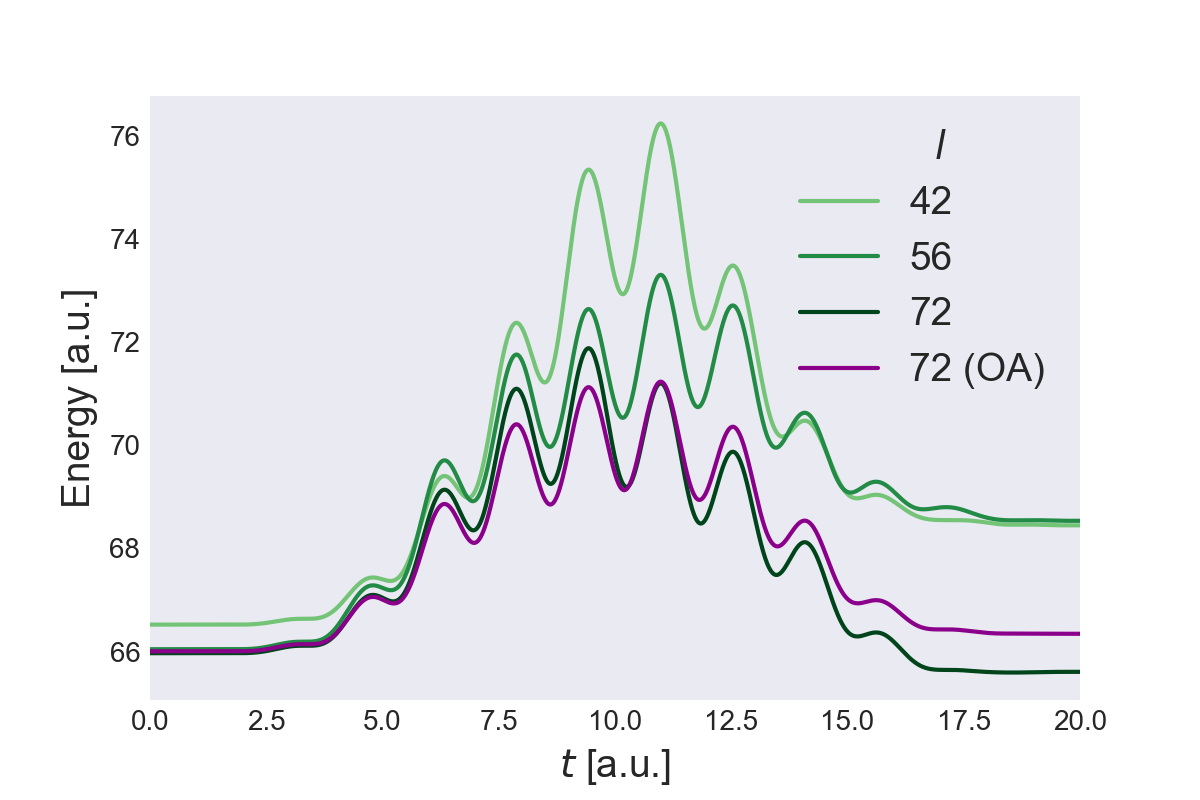
\includegraphics[width=0.75\textwidth]{results/figures/2D/n12_energy.png} 
    \caption{Time-dependent energy of a two-dimensional harmonic oscillator 
        with $n=12$ electrons under the influence of a laser field for different 
        spinorbitals $l\in\{42,56,72\}$.
    }
    \label{fig:n12_2d_energy}
\end{figure}

\begin{figure}
    \centering
    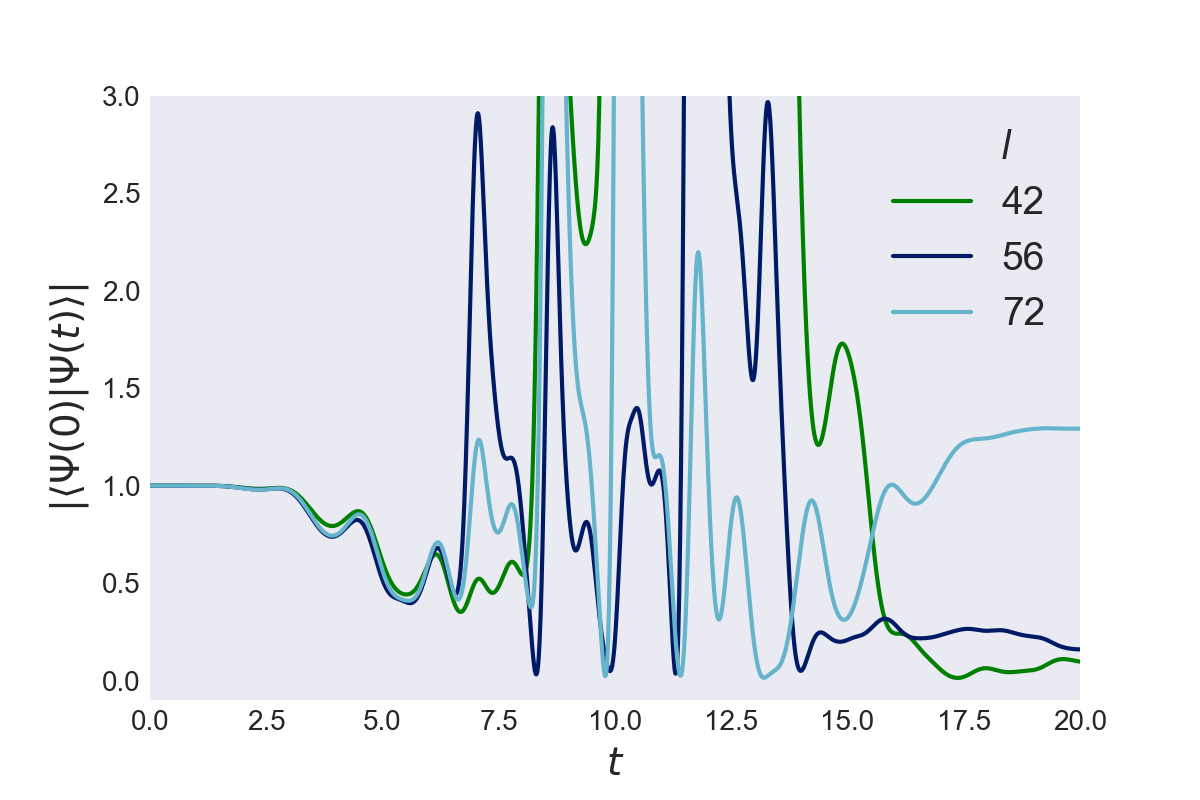
\includegraphics[width=0.75\textwidth]{results/figures/2D/n12_overlap.png} 
    \caption{Ground state probability $|\braket{\Psi(0)}{\Psi(t)}|^2$ for two-dimensional
        quantum dot with $n=12$ electrons under the influence of a laser field for 
        different number of spinorbitals $l=\{42,56,72\}$. 
    }
    \label{fig:n12_2d_overlap}
\end{figure}

The time-dependent energy of a two-dimensional harmonic quantum dot with $n=12$
electrons under influence of the oscillating field described above is shown in 
\autoref{fig:n12_2d_energy}. In this figure we have run the same simulation for 
$l\in\{42,56,72\}$ spin-orbitals with the time-dependent coupled cluster 
singles doubles (TDCCSD) method, and we see that only for the very largest of the 
basis set, we see a behaviour conforming with our expectations. We expect the 
energy to be close to the ground state energy after the laser-field has died down.

In the same figure (\autoref{fig:n12_2d_energy}) we have also included
the computed energy over time for the system using the
orbital-adaptive time-dependent coupled cluster doubles (OATDCCD) method and the 
same number if spin-orbitals.
We see that the two methods dont't agree completely, and we are prone to trust 
the OATDCCD method more than the TDCCSD method in this case, because the energy at 
the end of the simulations is lower than the initial energy for the TDCCSD method.
The reason for the problems the TDCCSD method shows are likely caused by our attempt 
to represent a state with the basis functions contained in the reference,
which is very dissimilar to said reference function. We will outline this problem 
further as we study the time-dependent ground state probability of the simulation.

The ground state probability of the same simulation with the TDDCCSD method 
is shown in
\autoref{fig:n12_2d_overlap}. We see immediately that the probability becomes 
non-sensical at some time step after $t=6 \text{ au}$. This result is similar to
the sort of break-down that occured for the TDCCSD method in the attempt to 
replicate the results of \citeauthor{miyagi2013time}\cite{miyagi2013time} in
\autoref{sec:miyagi_replication}.

The probable cause of the non-sensible 
ground state probability is the need for the amplitudes of the system to acquire 
relatively high values, in order to compensate for the inadequateness of the 
reference state to describe the exact time-dependent state. This is underlined 
by the norm of the amplitudes, displayed in \autoref{fig:n12_2d_amp_norms}. As 
is apparent, the lambda amplitudes shows an upwards trend throughout the 
simulation.
This should be unnecessary because the system would revert back to a state 
similar to the ground state at the end of the simulation. It appears that 
some ``tipping point'' is reached halfway around $t=T/2$ when instabillty 
increases. The $\tau$-amplitudes are more or less well-behaved, at least for 
the largest basis set, showing some correlation in amplitude with the
sinusoidal envelope of the oscillating field.

\begin{figure}
    \centering
    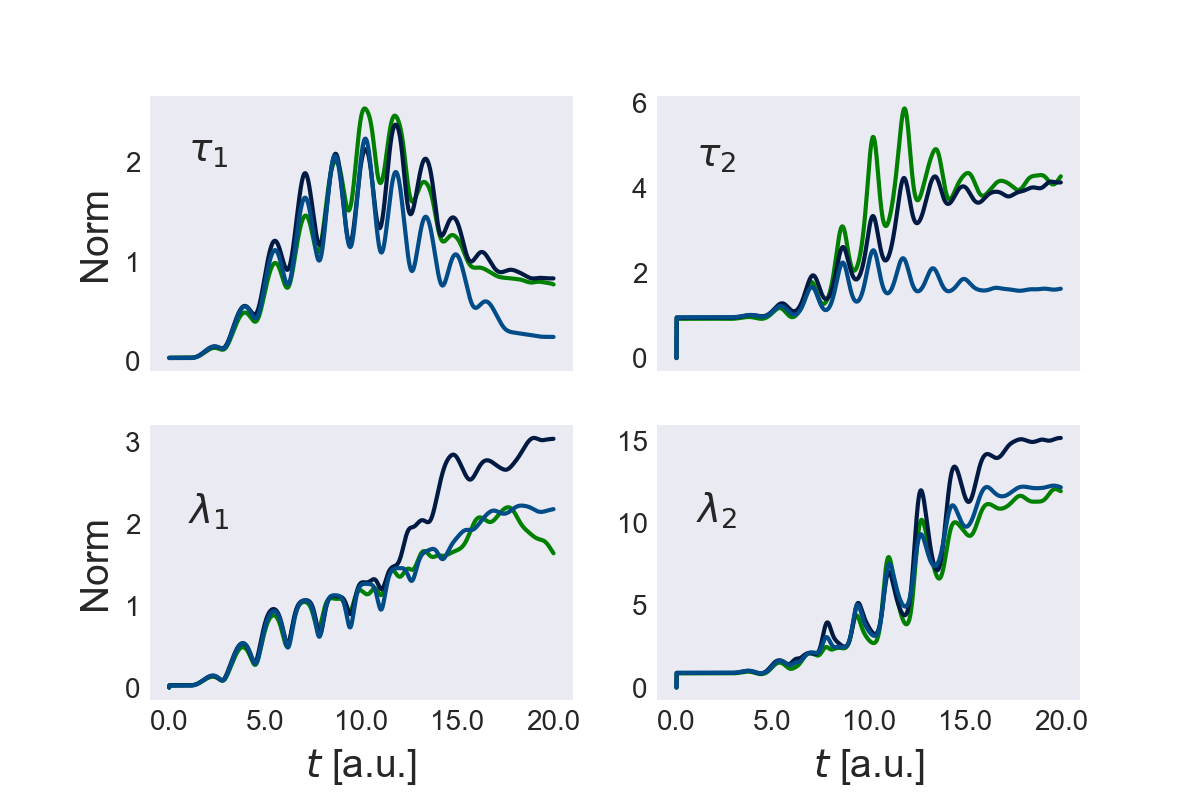
\includegraphics[width=0.9\textwidth]{results/figures/2D/n=12_amplitudes.png}
    \caption{Norm of amplitudes in a $n=12$ electron two-dimensional quantum 
        dot influenced by an oscilalting field, for several number of 
        spin-orbitals $l=\{42,56,72\}$.
    }
    \label{fig:n12_2d_amp_norms}
\end{figure}

\subsection{Dipole Spectrum}

We have for the two-dimensional quantum dot computed the dipole spectrum for systems of 
different size, like we did for the one-dimensional quantum dot. We did this for 
quantum dots with oscillator frequencies $\Omega=1$ with $n\in\{2,6,12\}$ electrons.
We used $l\in\{42,42,56\}$ as the number of spinorbitals for the respective systems.
In order to excite and disturb the systems from the intial ground state we applied 
an oscillating field with a resonant frequency $\omega=\Omega=1$ and a somewhat low 
maximum intensity $\vb{E}_\text{max}=0.1$, with a three-step linear envelope as 
in \autoref{eq:li_laser}. The systems were allowed to develop in time for 
$T = 500 \text{ au}$. The results of computing the Fourier transform of the 
dipole $\ev{x(t)} = \tr{\rho(t) x}$ is depicted in \autoref{fig:2d_dipole_spectra}. 
In this figure we see that the result is qualtitatively in accordance with the 
harmonic potential theorem - the dipole freqcuencies of all the systems are the 
same, with an intensity that increases with the number of particles in the system.
For the two larger systems with $n=6$ and $n=12$ electrons we see some slight 
inccuracies. These are attributable to the time constraint of this study - 
a simulation with larger number of spinorbitals would have remedied these 
inaccuracies, but would have needed more time to complete.

\begin{figure}
    \centering
    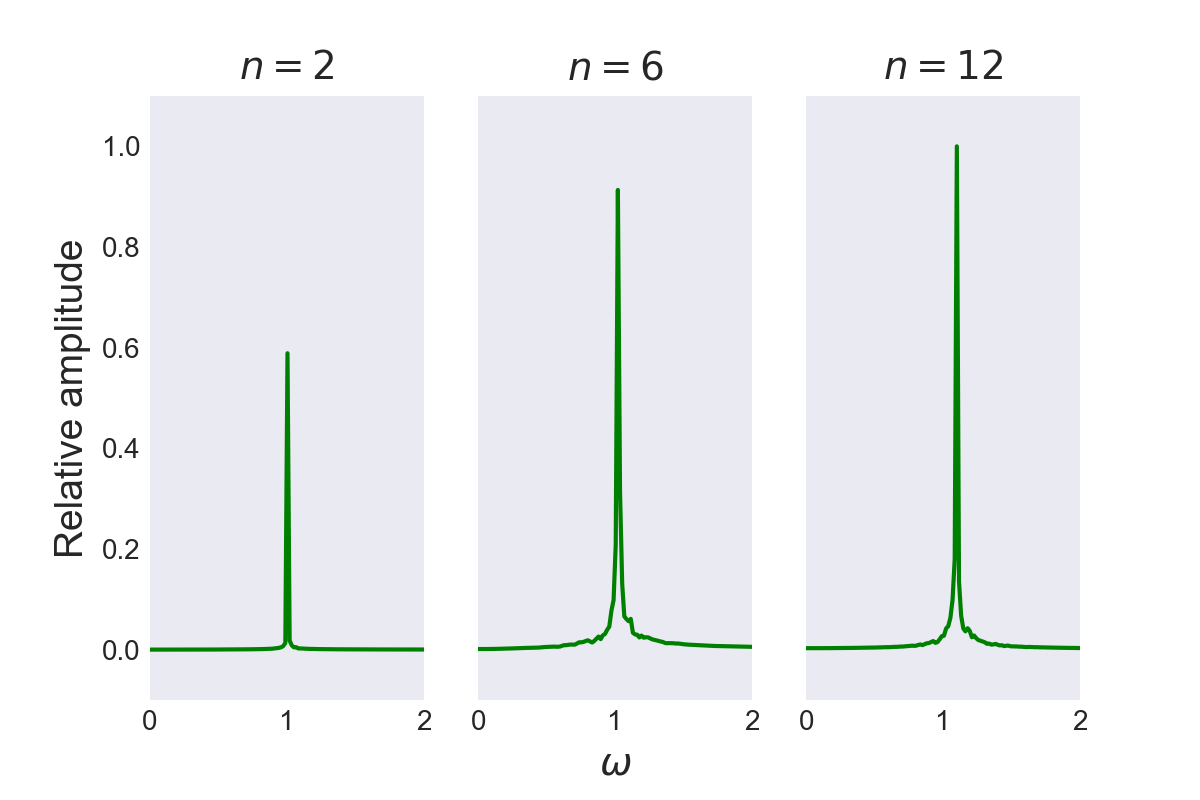
\includegraphics[width=0.8\textwidth]{results/figures/2D/2d_spectrum.png} 
    \caption{Fourier transform of expected value of dipole moment for a
        two-dimensional quantum dot with different number of electrons 
        $n=\{2,6,12\}$ and respective number of spin-orbitals 
        $l=\{40,40,56\}$.
    }
    \label{fig:2d_dipole_spectra}
\end{figure}

\subsection{Resonance Sensitivity}

For the two-dimensional quantum dot we have also conducted a resonance sensitivity analysis,
similar to the one we performed for the one-dimensional quantum dot. The results for 
$n=2$ electrons and $n=6$ electrons are displayed in \autoref{fig:2d_resonance_n2}
and \autoref{fig:2d_resonance_n6} respectively. The quantum dots in these simualtions 
had an oscillator frequency of $\Omega=1$ and where subjected to an oscillating 
field with a sinusoidal envelope of the type in \autoref{eq:results_1d_field} of 
different frequencies $\omega\in\{1.0,1.25,1.5,1.75,2.0\}$ and a maximum intensity of 
$\vb{E}_\text{max}=0.25$. The simulations were done with the time-dependent coupled 
cluster doubles (TDCCSD) method with static orbitals.

Like in the one-dimensional analysis we see that the systems are much more prone to 
excitation as the frequency of the laser field approaches that of the quantum harmonic 
oscillator. This is apparent both for the energy of the quantum dot systems and the 
ground state probabilites displayed in the left and right subfigures of
\autoref{fig:2d_resonance_n2} and \autoref{fig:2d_resonance_n6}, respectively. In the 
six-particle case we again see the problems with the TDCCSD method when computing the 
ground state overlap, as the amplitudes acquire higher and higher values, resulting 
in non-sensical probability values. In this case we do believe the 
energy plots to be correct for $\omega\in\{1.5, 1.75,2.0\}$. The energies for the last 
two oscillating field frequencies, $\omega\in\{1.0,1.25\}$, we have less trust in because 
of the non-sensical time-dependent ground state probabilities.

\begin{figure}
    \centering
    \begin{minipage}{0.49\textwidth}
        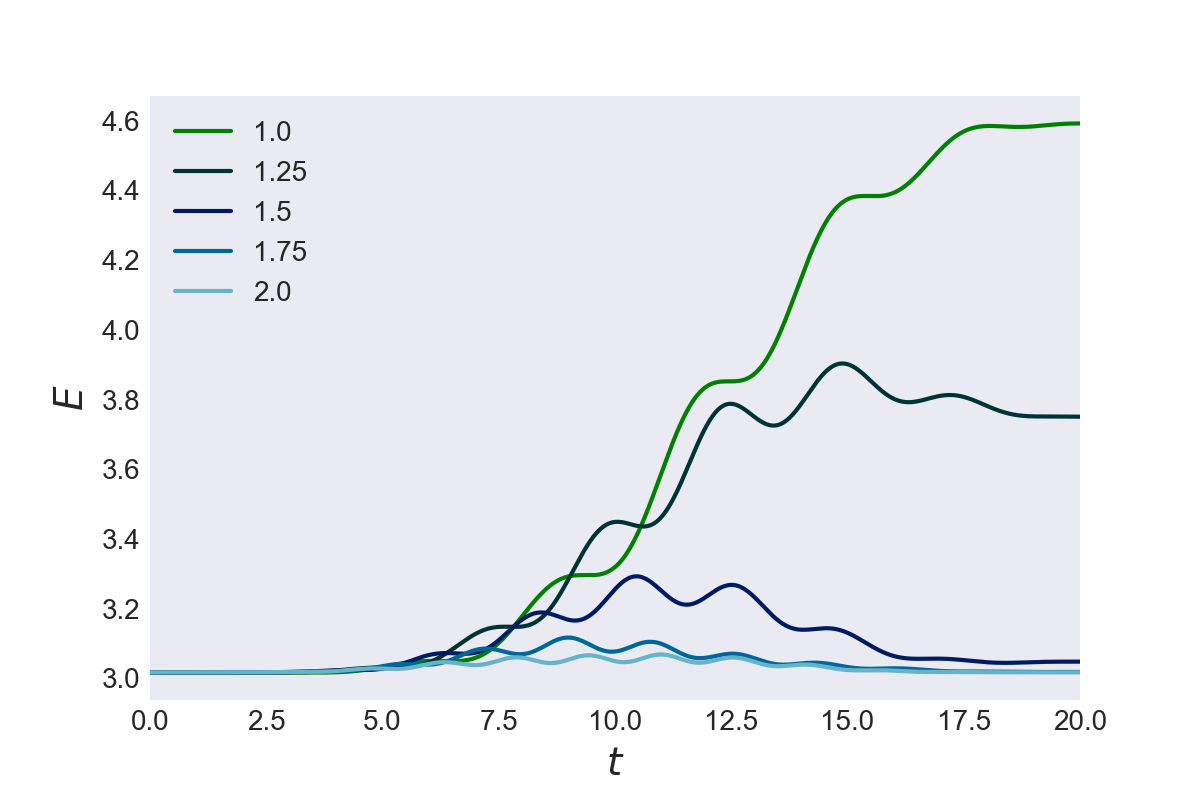
\includegraphics[trim=2em 0em 5em 0em, width=\textwidth]{results/figures/2D/resonance/n2resonance.png} 
    \end{minipage}\hfill
    \begin{minipage}{0.49\textwidth}
        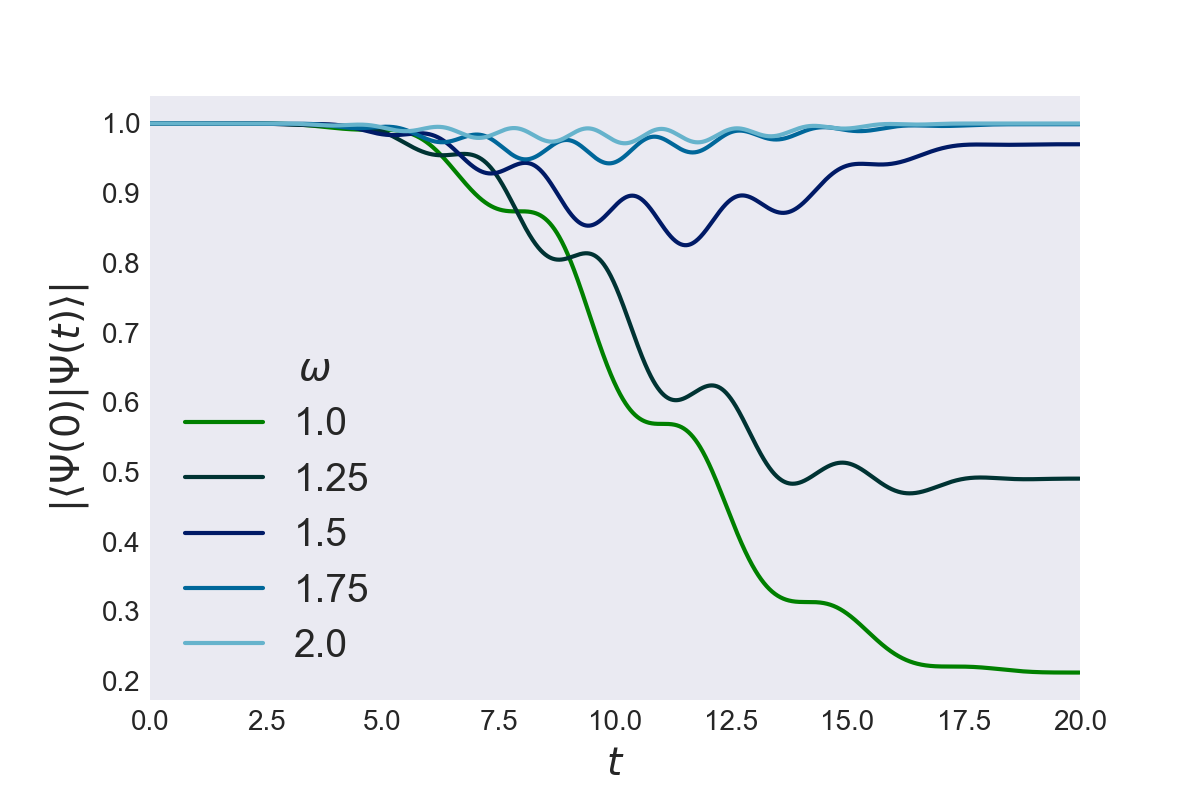
\includegraphics[trim=0em 0em 5em 0em, width=\textwidth]{results/figures/2D/resonance/n2overlap_res.png} 
    \end{minipage}
    \caption{Time dependent energy (left) and ground state probability $|\braket{\Psi(0)}{\Psi(t)}|^2$
        (right) for a two-dimensional quantum dot with $n=2$ electrons. The quantum dot 
        is affected by an oscillating field of different frequencies
        $\omega\in\{1.0, 1.25, 1.5, 1.75, 2.0\}$ with a maximum inntensity
        $\vb{E}_\text{max} = 0.25$. The confining harmonic potential has frequency $\Omega=1$.
    }
    \label{fig:2d_resonance_n2}
\end{figure}

\begin{figure}
    \centering
    \begin{minipage}{0.49\textwidth}
        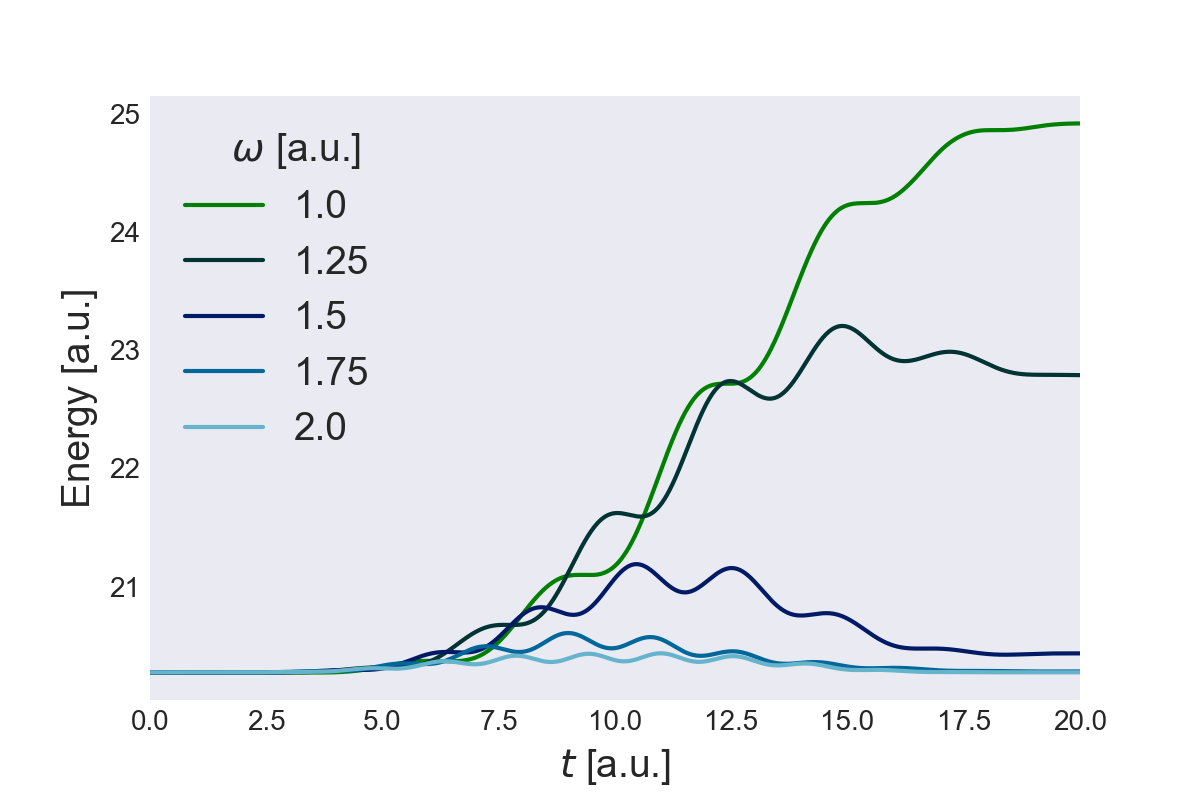
\includegraphics[trim=2em 0em 5em 0em, width=\textwidth]{results/figures/2D/resonance/n6resonance.png} 
    \end{minipage}\hfill
    \begin{minipage}{0.49\textwidth}
        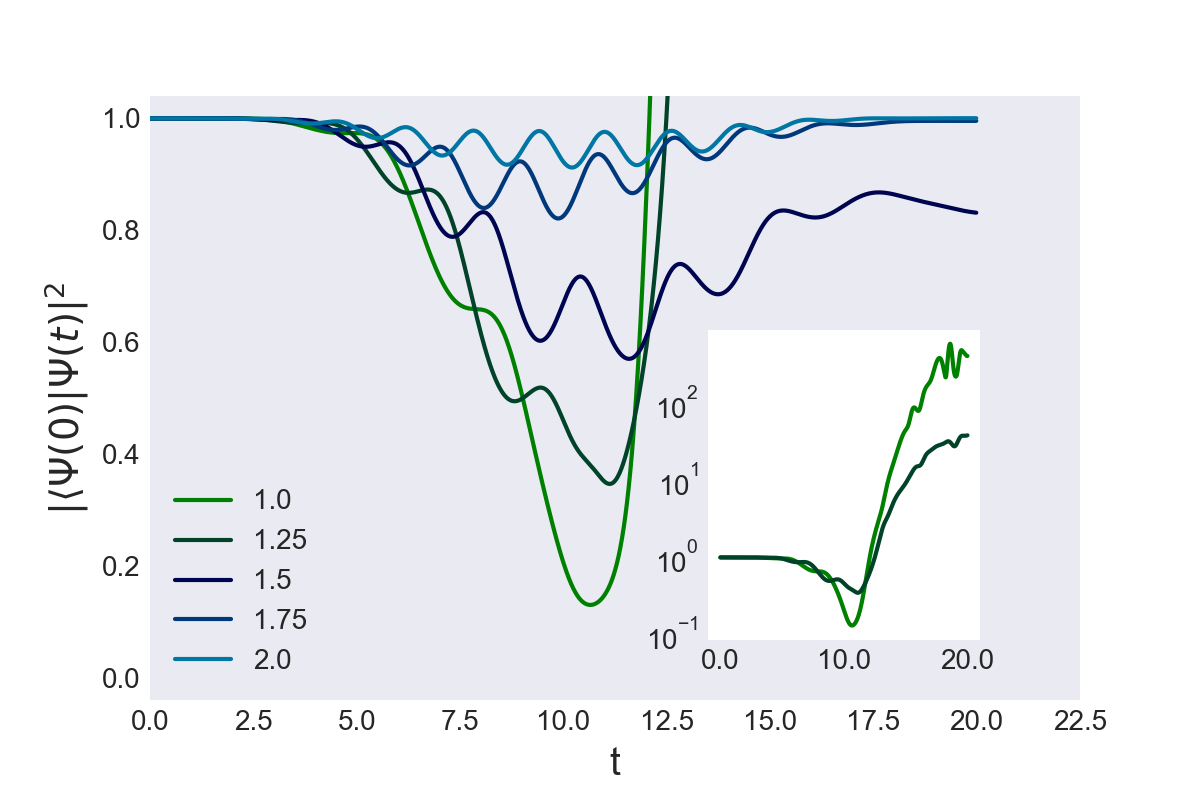
\includegraphics[trim=0em 0em 5em 0em, width=\textwidth]{results/figures/2D/resonance/n6_overlap_res.png} 
    \end{minipage}
    \caption{Time dependent energy (left) and ground state probability $|\braket{\Psi(0)}{\Psi(t)}|^2$
        (right) for a two-dimensional quantum dot with $n=6$ electrons. The quantum dot 
        is affected by an oscillating field of different frequencies
        $\omega\in\{1.0, 1.25, 1.5, 1.75, 2.0\}$ with a maximum inntensity
        $\vb{E}_\text{max} = 0.25$. The confining harmonic potential has frequency $\Omega=1$.
    }
    \label{fig:2d_resonance_n6}
\end{figure}


\section{Two-dimensional Double Dot}

We have simulated two different two-dimensional double dot systems, one with $n=2$ electrons 
and 
one system with $n=4$ electrons, using the \lstinline{TwoDimensionalDoubleWell} class described
in \autoref{sec:2d_double_well}. We use $l=20$ spin-orbitals for the two-electron system 
and $l=56$ spin-orbitals for the four-electron system. The class requires two special parameters, 
\lstinline{l_ho_factor} and \lstinline{barrier_strength}, that define the 
number of regular harmonic oscillator functions to map to and the height of the 
barrier in the middle of the well, respectively. We set the barrier strength to $2$ 
and the harmonic oscillator factor to $2$ for both systems. The oscillator frequency 
of the double dot is set to $\Omega=1$. As a visual confirmation of the systems, a 
one-electron density plot is provided for the $n=2$ electrons system (left) and 
the $n=4$ electron system (right) in \autoref{fig:2d_dw_rho}. We see from these density plots 
that the repulsive Couloumb interacting has a stronger effect for the system with the 
highest number of electrons.

The double dot is in essence a perturbation of the regular two-dimensional quantum dot,
and we are seeking to uncover any many-body 
effects that such a perturbation could lead to. In order to do this we would like to 
compute the dipole spectrum of both systems. The time-propagation is done using the 
orbital-adaptive time-dependent coupled cluster doubles (OATDCCD) method, as it has shown 
the best stability of our time-dependent methods. Both systems are under the influence of an 
oscillating field with a linearly decreasing- and increasing envelope of the type used by 
\citeauthor{li2005time}\cite{li2005time} (\autoref{fig:li_compare}). We have chosen a 
frequency of this field that corresponds to the resonant of the first transition energy 
of the system $\omega = 0.43 \text{ au}$, and an intensity yielding a maximum amplitude
$\vb{E}_\text{max} = 0.1 \text{ au}$. The resonant frequency was found by direct diagonalisation 
of the one-body matrix produced by the system class \lstinline{TwoDimensionalDoubleWell}.

\begin{figure}
    \centering
    \begin{minipage}{0.49\textwidth}
        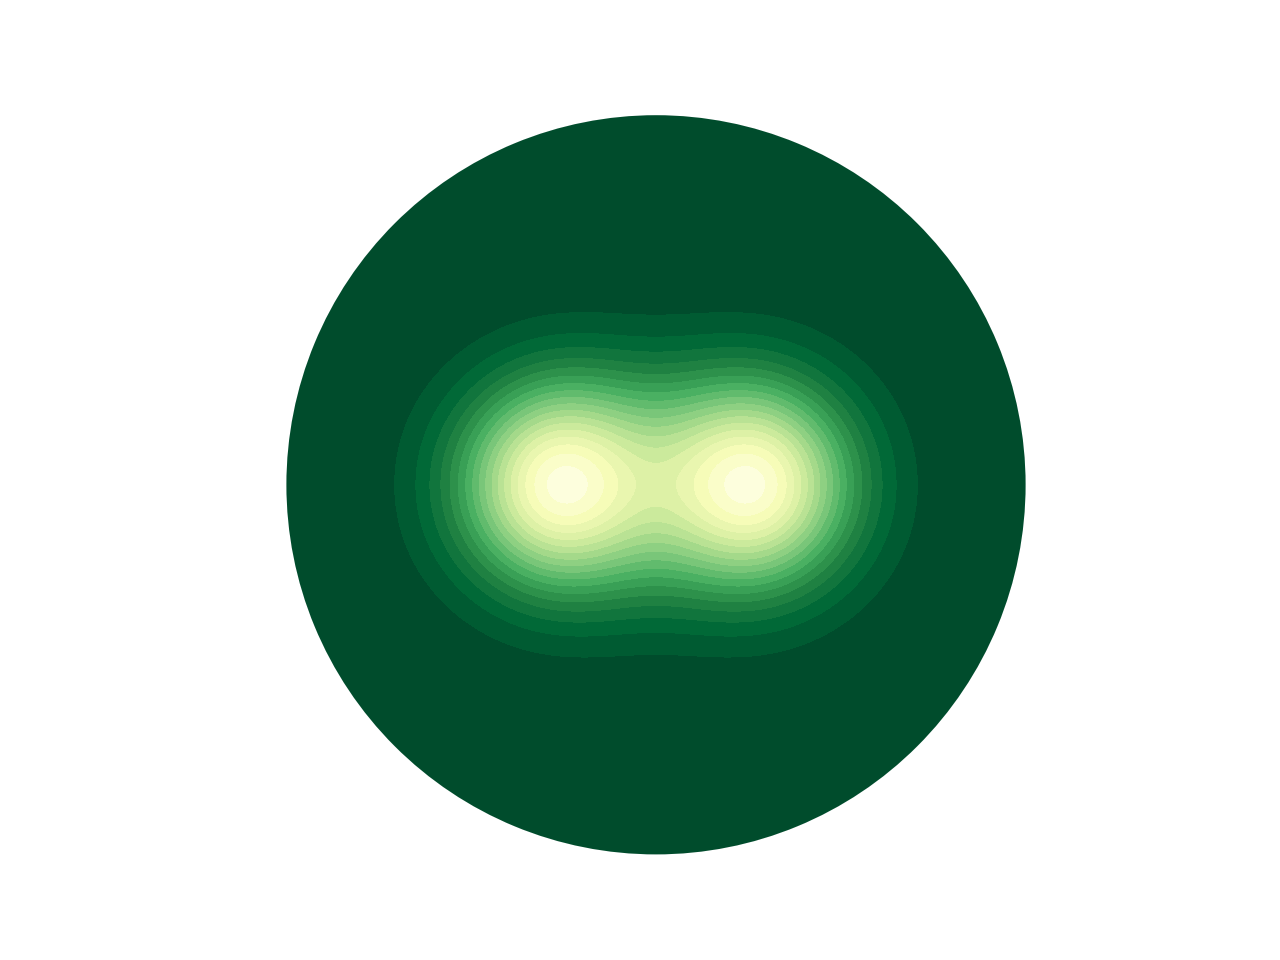
\includegraphics[trim=4em 3.5em 4em 4em, clip=true, width=\textwidth]{results/figures/DW/rho_dw.png} 
    \end{minipage}\hfill
    \begin{minipage}{0.49\textwidth}
        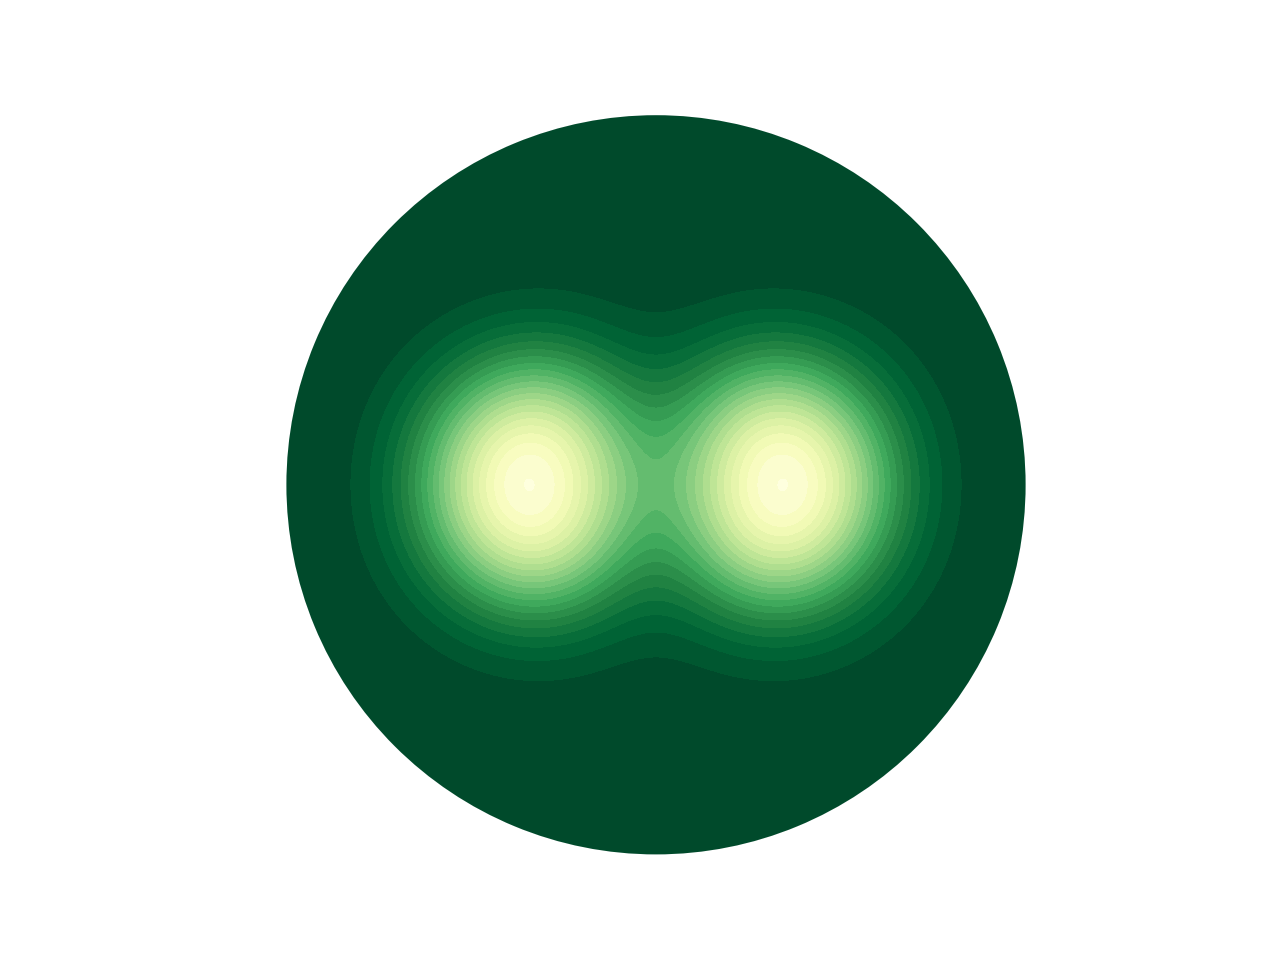
\includegraphics[trim=4em 3.5em 4em 4em, clip=true, width=\textwidth]{results/figures/DW/rho_dw_n4.png} 
    \end{minipage}
    \caption{Ground state one-electron density for $n=2$ electrons (left)
        and $n=4$ electrons (right) for a double quantum dot.
    }
    \label{fig:2d_dw_rho}
\end{figure}

\begin{figure}
    \centering
    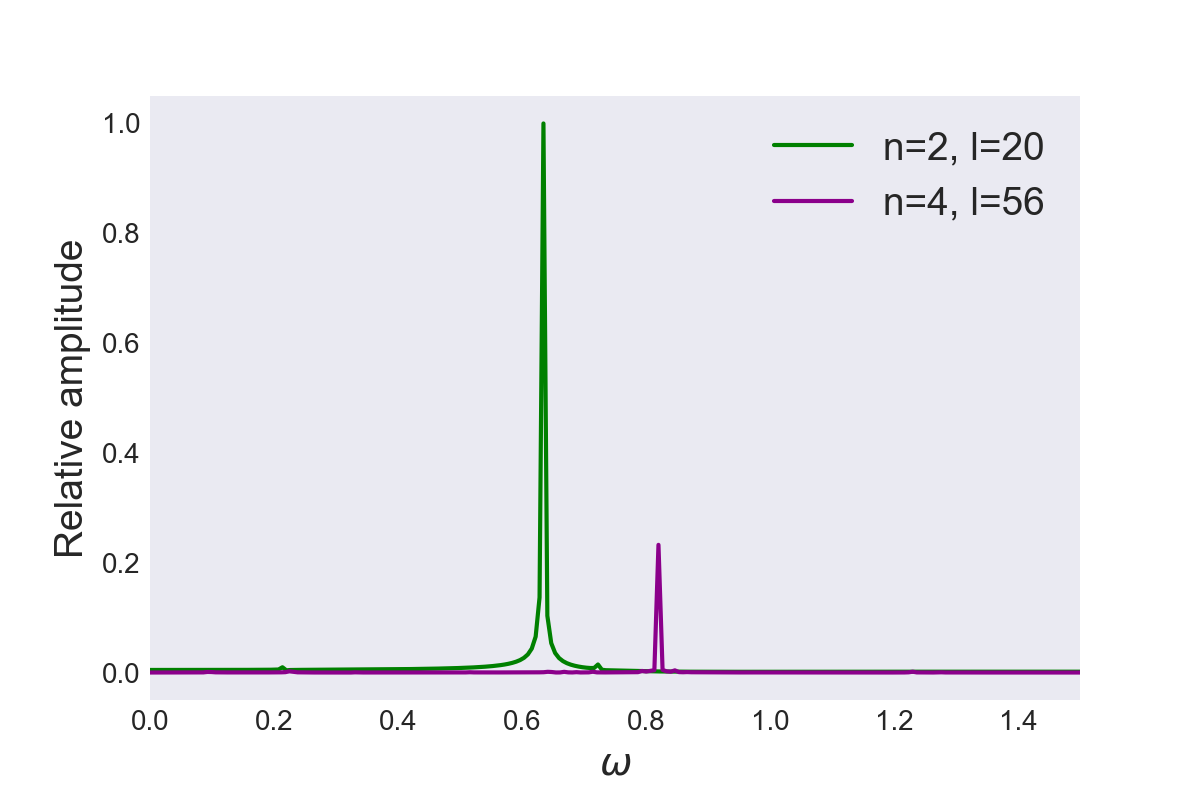
\includegraphics[width=0.75\textwidth]{results/figures/DW/dw_n2_n4_spectrum.png} 
    \caption{Dipole spectrum of two-dimensional double dot system with $n\in\{2,4\}$
        electrons and $l\in\{20, 56\}$ spinorbitals. 
    }
    \label{fig:2d_dw_n2_n4_spectra}
\end{figure}

The system is allowed to develop in time for $T = 100 \text{ au}$ and then we compute the Fourier 
transform of the dipole moment $\ev{\hat{x}(t)} = \tr{\rho(t) x}$, the results of which are shown 
in \autoref{fig:2d_dw_n2_n4_spectra}. We immediately see that there is only one frequency 
apparent in the spectra for each of the systems, meaning that the quantum double dots
have a position operators that behave as if it was the centre of mass of the system. We 
see that the larger system has a somewhat higher value for the one frequency in the spectrum 
compared with the smaller system. We also see that the larger system has lower intensity compared
with the smaller 
system.

This difference in frequency of the two systmes may be caused by the increased Coulomb force
creates a higher effective potential that contrains the electrons to the two wells.
The lower intensity of the larger system may also be explained by the same higher-potential effect 
of the Coulomb force, but can also be attributed to the fact that there is more mass to move with 
the same intensitivity of the external field. We find this decrease in intensity somewhat puzzling,
as the same laser field applied to a larger system would yield an increase for the the single-well 
potential.

We may have seen more many-body effects in the form of more spectral lines if we were to increase 
the intensity of the oscillating laser field, decrease the barrier strength of the double well potential,
or both. This may have made it more likely to tunnel through the barrier, i.e. increase transition 
probabilities of higher energy quantum leaps. With the methods at hand we have had problems with 
convergence of our solvers for very large field strenght, however. We sought to remedy this by 
implementing a smoother double well potential, but had to abandon this effort due to the time 
restriction of this thesis.


\section{Two-dimensional Magnetic Quantum Dot}

We start the study of two-dimensional quantum dots under the influence of a magnetic 
field by defining a system of only one particle and solving the time-dependent 
Schrödinger equation
directly. This is a accomplished by using the \lstinline{TwoDimHarmonicOscB} class
to produce a basis set and dipole elements
which is everything we need. All of these items are properties of the class and can be
easily extracted. A simple periodic function that simulates an electric field is constructed, as 
the product of such a time-dependent operator and the interaction matrix defines the 
time propagation. We then use a simple integration scheme, in this case the fourth-order 
Runge-Kutta method, to propagate the ground state single particle function of the system.
Taking care to extract the dipole for every time step, we can compute the discrete Fourier 
transform of the dipole and compute the frequency spectrum of our system. This procedure is 
applied to a system completely absent of a magnetic field, and a system under direct influence 
of a magnetic field.

Before going straight to the results, we study the shell structure and allowed transitions of 
our two systems. The left part of \autoref{fig:shell_structure_yes_no_b} presents the 
shell structure of a the regular two-dimensional quantum dot. The states have all been assigned
a number for easier examination. This shell structure is 
identical to the one presented in \autoref{fig:2d_basis_states}. Additionally, here we have added
coloured double arrows to illustrate the allowed transitions in the quantum dot. These 
transitions can be encountered in the transition matrix for the system, which is
reproduced with color coding in \autoref{fig:transition_no_b}. Notice that the coloured 
arrows representing allowed transitions match in colour with the elements of the transition 
matrix.

\begin{figure}
    \begin{center}
    \begin{tikzpicture}[scale=0.9, background rectangle/.style={fill=grey},
        show background rectangle]
    \begin{scope}
      
        % TOP
        \foreach \i in {0, 3, 6} {
            \draw(\i, 2) -- (\i + 2, 2);
            \node at (\i + 0.75, 2) {$\uparrow$};
            \node at (\i + 1.25, 2) {$\downarrow$};
        }
       
        \node[below, inner sep=.5em] at (1, 2) {$(0, -2)$};
        \node[above] at (1, 2) {5};
        \node[below, inner sep=.5em] at (4, 2) {$(1, 0)$};
        \node[above] at (4, 2) {3};
        \node[below, inner sep=.5em] at (7, 2) {$(0, 2)$};
        \node[above] at (7, 2) {4};

        % MIDDLE
        \foreach \i in {1.5, 4.5} {
            \draw(\i, 1) -- (\i + 2, 1);
            \node at (\i + 0.75, 1) {$\uparrow$};
            \node at (\i + 1.25, 1) {$\downarrow$};
        }

        \node[below, inner sep=.5em] at (2.5, 1) {$(0, -1)$};
        \node[above] at (2.5, 1) {1};
        \node[below, inner sep=.5em] at (5.5, 1) {$(0, 1)$};
        \node[above] at (5.5, 1) {2};

        % BOTTOM
        \draw(3, 0) -- (5, 0);
        \node at (3 + 0.75, 0) {$\uparrow$};
        \node at (3 + 1.25, 0) {$\downarrow$};

        \node[below, inner sep=.5em] at (4, 0) {$(0, 0)$};
        \node[above] at (4, 0) {0};

        % Transitions
        \draw [<->, line width=.1em, transition11] (3.5, 0) -- (3.25, 1);
        \draw [<->, line width=.1em, transition11] (4.5, 0) -- (4.75, 1);

        \draw [<->, line width=.1em, transition12] (3, 1) -- (3.25, 2);
        \draw [<->, line width=.1em, transition12] (5, 1) -- (4.75, 2);

        \draw [<->, line width=.1em, transition13] (2, 1) -- (1.75, 2);
        \draw [<->, line width=.1em, transition13] (6, 1) -- (6.25, 2);

    \end{scope}

    \begin{scope}[xshift=20em]

        % MIDDLE 2
        \foreach \i in {1.5, 4.5} {
            \draw(\i, 3) -- (\i + 2, 3);
            \node at (\i + 0.75, 3) {$\uparrow$};
            \node at (\i + 1.25, 3) {$\downarrow$};
        }

        \node[below, inner sep=.5em] at (2.5, 3) {$(1, 0)$};
        \node[above] at (2.5, 3) {3};
        \node[below, inner sep=.5em] at (5.5, 3) {$(0, 3)$};
        \node[above] at (5.5, 3) {6};

        % MIDDLE 1
        \foreach \i in {1.5, 4.5} {
            \draw(\i, 2) -- (\i + 2, 2);
            \node at (\i + 0.75, 2) {$\uparrow$};
            \node at (\i + 1.25, 2) {$\downarrow$};
        }

        \node[below, inner sep=.5em] at (2.5, 2) {$(0, -1)$};
        \node[above] at (2.5, 2) {1};
        \node[below, inner sep=.5em] at (5.5, 2) {$(0, 2)$};
        \node[above] at (5.5, 2) {4};

        % BOTTOM 2
        \draw(3, 1) -- (5, 1);
        \node at (3 + 0.75, 1) {$\uparrow$};
        \node at (3 + 1.25, 1) {$\downarrow$};

        \node[below, inner sep=.5em] at (4, 1) {$(0, 1)$};
        \node[above] at (4, 1) {2};
        
        % BOTTOM 1
        \draw(3, 0) -- (5, 0);
        \node at (3 + 0.75, 0) {$\uparrow$};
        \node at (3 + 1.25, 0) {$\downarrow$};

        \node[below, inner sep=.5em] at (4, 0) {$(0, 0)$};
        \node[above] at (4, 0) {0};
        
        % Transitions 

        % 0 -> 1
        \draw [<->, line width=.1em, transition21] (3.5, 0) to[out=120, in=-90] (1.75, 2);
        % 0 -> 2
        \draw [<->, line width=.1em, transition21] (4.5, 0) -- (4.5, 1);

        % 2 -> 3
        \draw [<->, line width=.1em, transition23] (3.5, 1) to[out=60, in=-50] (3.25, 3);
        % 2 -> 4
        \draw [<->, line width=.1em, transition22] (4.75, 1) -- (4.75, 2);

        % 1 -> 3
        \draw [<->, line width=.1em, transition23] (2, 2) -- (2, 3);
        % 4 -> 6 
        \draw [<->, line width=.1em, transition24] (6, 2) -- (6, 3);

    \end{scope}
    \end{tikzpicture}
    \end{center} 
    \caption{Shell structure of six lowest orbitals before (left), and after (right)
        a magnetic field is applied to a 2D quantum dot.}
    \label{fig:shell_structure_yes_no_b}
\end{figure}

When we apply apply a magnetic field of strength $\omega_c/\omega = \sqrt{2}/2$ we 
obtain the shell structure represented to the right in 
\autoref{fig:shell_structure_yes_no_b}, where the allowed transitions correpsond to the 
transition matrix in \autoref{fig:transition_yes_b}. The chosen magnetic field strength 
was not chosen arbitrarily, as these accidental degenracies occur only rarely as 
a function of magnetic field strength\footnote{Hence the term ``accidental''.}.
For succinctness we repeat the function for energy eigenvalues for two-dimensional 
quantum dot influenced by a magnetic field (\autoref{eq:2d_b_eigenvalues}),
\begin{equation}
    \epsilon_{nm} = \hbar\Omega(2n + |m| + 1) - \frac{\hbar\omega_c}{2}m,
\end{equation}
where $\Omega = \sqrt{\omega_0^2 + \frac{\omega_c^2}{4}}$.
Apart from a general shift up in energy by adding a magnetic field, the states with 
negative azimuthal quantum number $m$ will experience an increase in energy eigenvalue,
and vice versa. We see this effect clearly in the new shell structure in
\autoref{fig:shell_structure_yes_no_b}. The states with negative $m$ have indeed
undergone a relative shift upwards, whilst the states with positive $m$ have been
shifted downwards, relative to the other states. The ground state, labelled 0, 
remains relatively stationary, the states labelled 2 ($m=1$) and 4 ($m=2$) have been 
shifted downwards and the states labelled 1 ($m=-1$) and 5 ($m=-2$) have been shifted 
upwards. State number 5 so much that it has disappeared from the shell structure, with a 
new state 6 ($=3$) appearing. This is due to our restriction to include only the six
lowest-energy orbitals. We see that the possible remaining allowed transitions remain the 
same, with the exception of transitioning between state 1 and 5, because state 5 is no more,
and the addition of a possible transition between state 4 and 6.

\begin{figure}
    \begin{center}
    \begin{minipage}{0.4\textwidth}
        \centering
        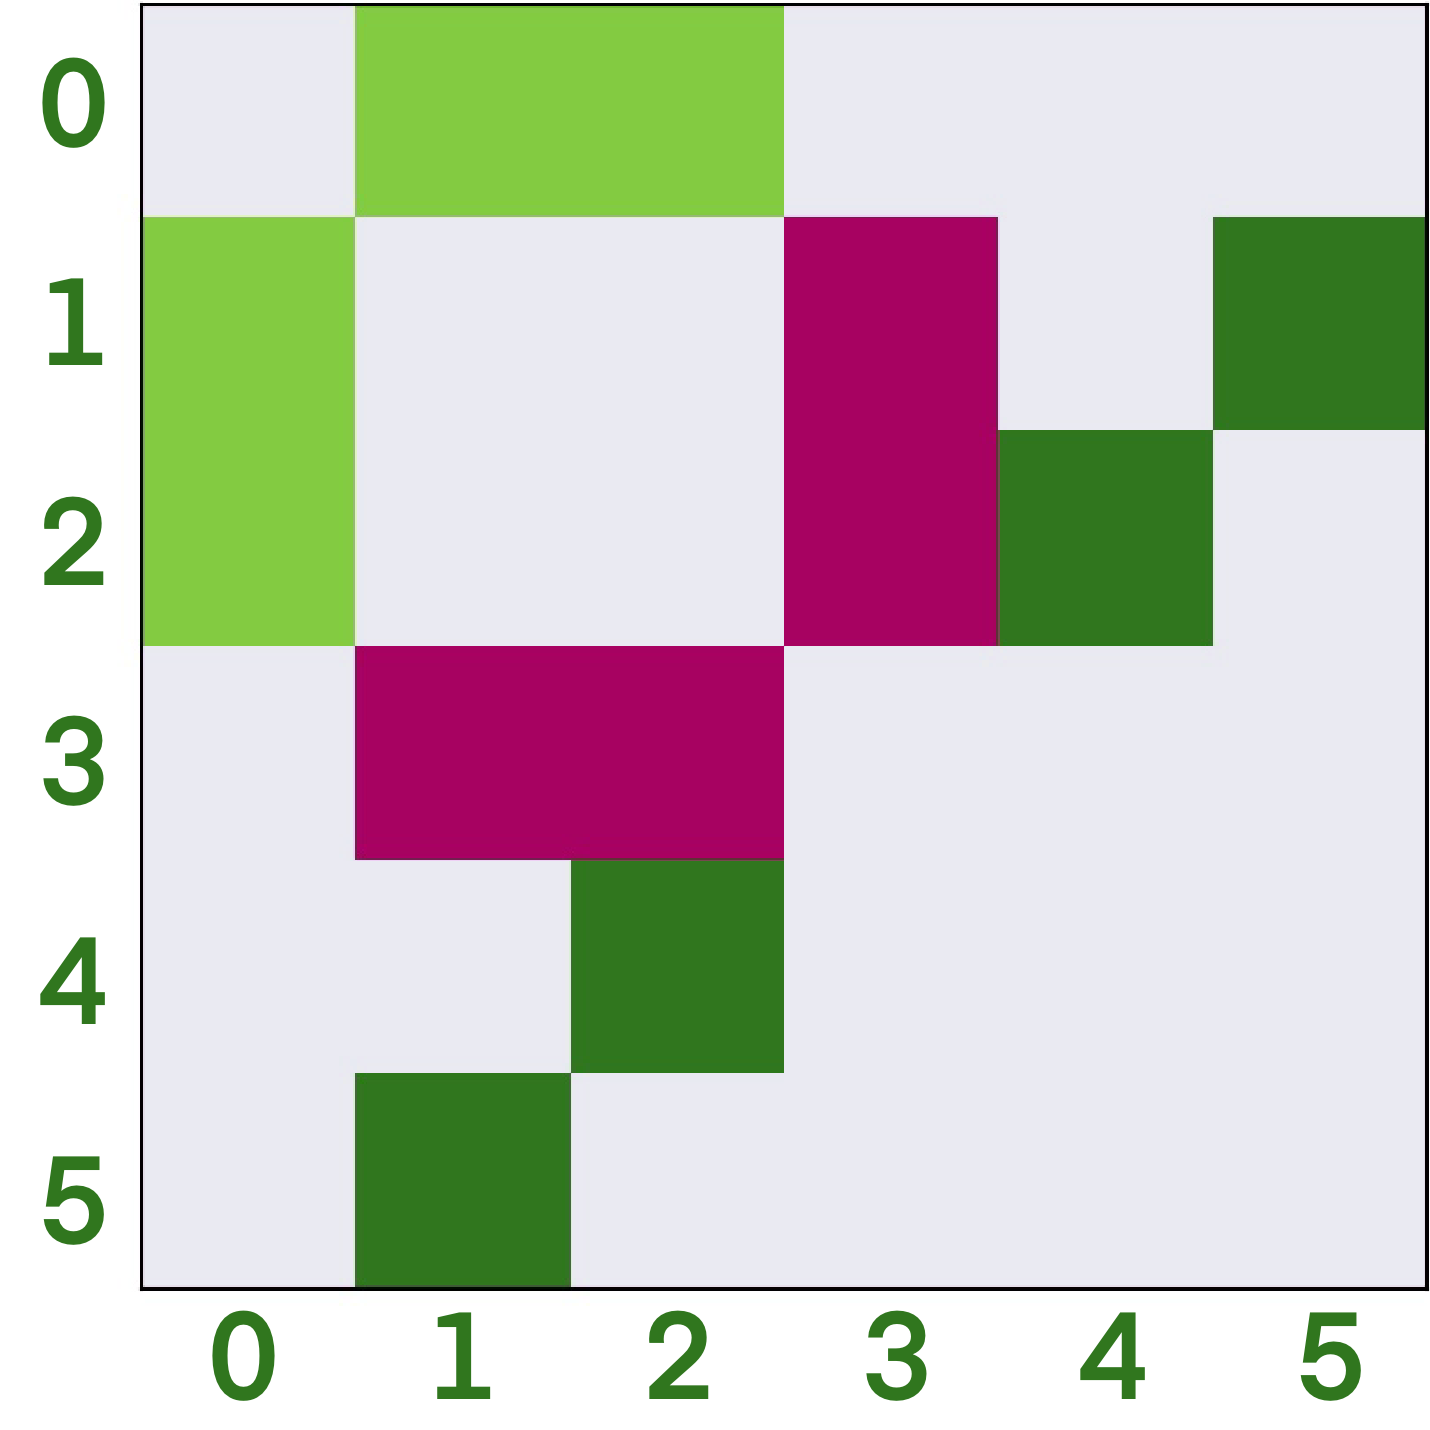
\includegraphics[width=\textwidth]{results/figures/dipole_no_b.png}
        \caption{Transition matrix dictating the allowed transitions for a
            2D quantum dot.}
        \label{fig:transition_no_b}
    \end{minipage}
    \begin{minipage}{0.4\textwidth}
        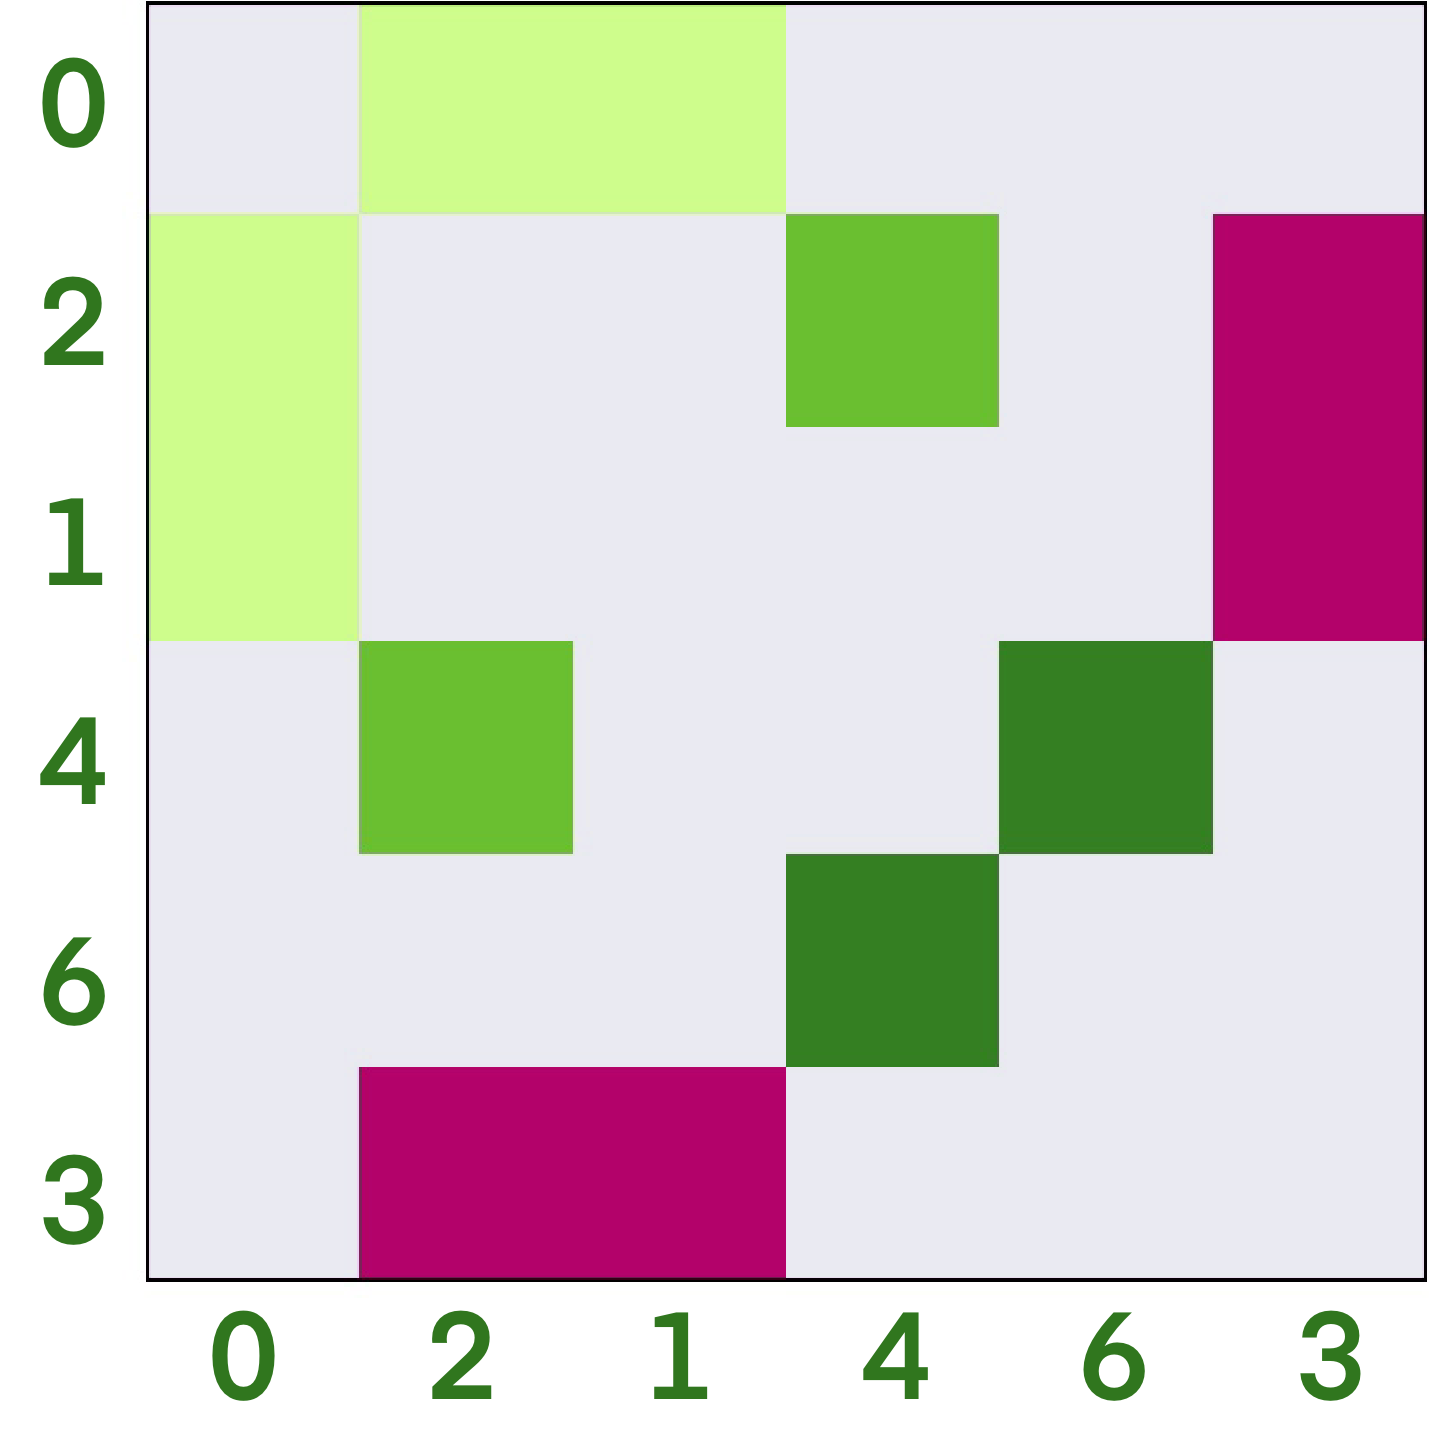
\includegraphics[width=\textwidth]{results/figures/dipole_yes_b.png}
        \caption{transition matrix for a 2D quantum dot when a magnetic field
            is applied.}
        \label{fig:transition_yes_b}
    \end{minipage}        
    \end{center}
\end{figure}

If we compute the frequency spectrum of the two systems
(\autoref{fig:transmission_spectrum_b_field}) we get a single line for the 
normal quantum dot. This is expected, as the quantum harmonic oscillator has 
the same energy difference between each level. However, when we apply a magnetic
field and shift the energies of the orbitals in the quantum dot, we see that we 
get two different energy transitions. This is revealed as two lines in the 
frequency spectrum in \autoref{fig:transmission_spectrum_b_field}. This is equivalent 
to a splitting in transmisstion spectra of quantum dot arrays under the effect 
of a magnetic field in experiments\cite{heitmann1993spectroscopy,meurer1992single}.

\begin{figure}
    \centering
    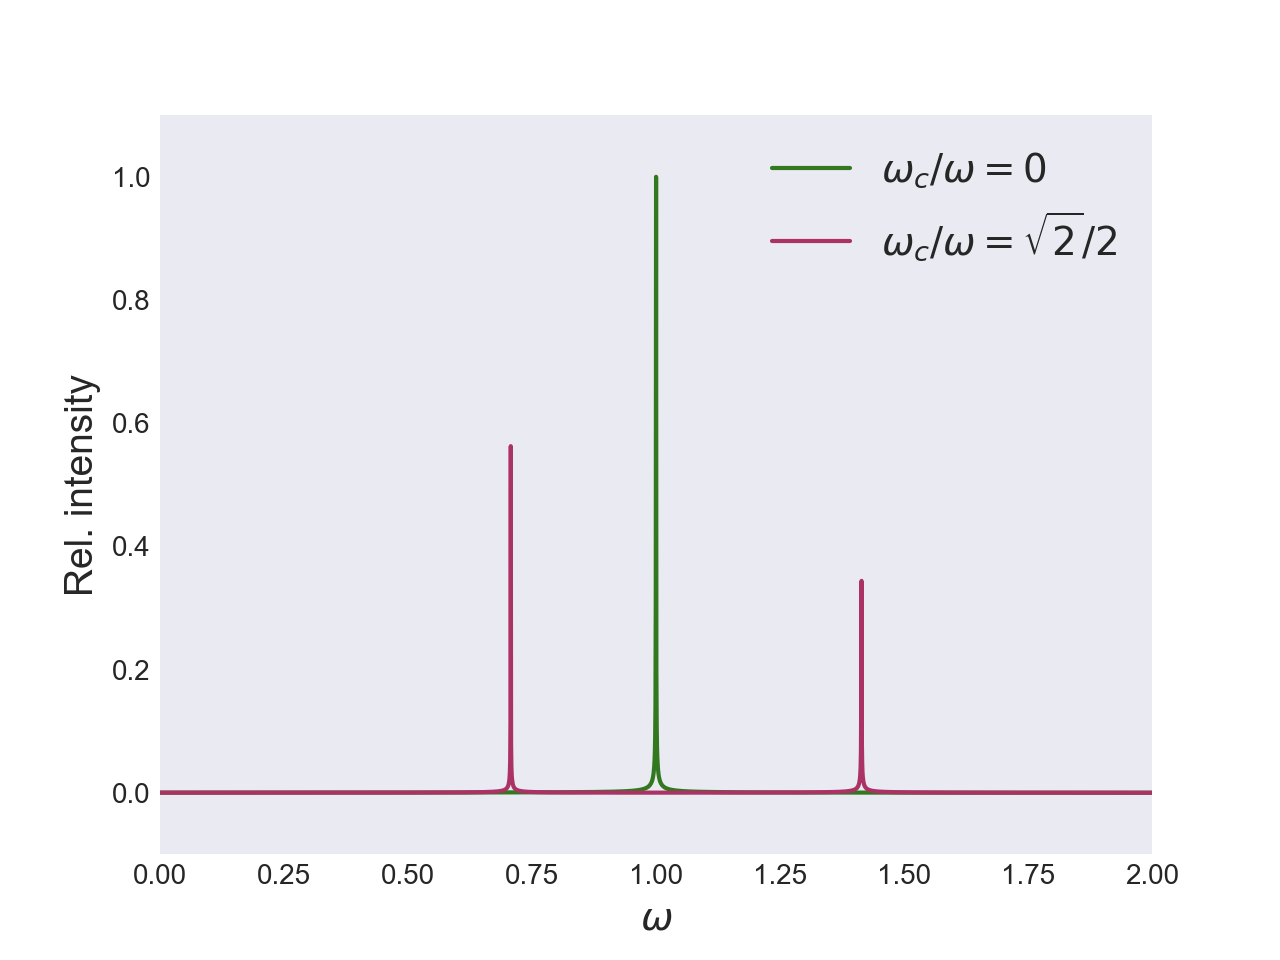
\includegraphics[width=0.75\textwidth]{results/figures/transmission_spectrum.png}
    \caption{Spectrum of a single-electron two-dimensional quantum dot both with and
        without a magnetic field.
    }
    \label{fig:transmission_spectrum_b_field}
\end{figure}

\subsection{Many-particle Magnetic Quantum Dots}

We will now show that the dipole spectrum splitting holds for a quantum dot of 
several electrons. To do this we conduct several simulations of quantum dots consisting 
of both $n=2$ and $n=4$ electrons. Because of the reordering of quantum degeneracies 
that occurs by introducing a magnetic field, we will not run into any multi-reference 
problems for the $n=4$ electron case.

The quantum dot systems are each excited by a laser pulse with the linearly increasing 
and decreasing envelope, as defined by \citeauthor{li2005time}\cite{li2005time}, in 
equation \autoref{eq:li_laser}. The laser of this oscillating field is set to the 
same frequency as the system $\omega=\omega_0=1$ and the maximum intensity of the field 
is $\vb{E}_\text{max} = 0.1$. The Larmor frequency of the magnetic field that the 
quantum dots are subjected to is varied, $\omega_c\in\{0.25, 0.5, 0.75, 1.0\}$.
For each of these simulations we compute the Fourier transform of the dipole in 
the same direction as the polarisation of the laser field, $\ev{x} =\tr{\rho x}$.
In the simulations with $n=2$ electrons we used $l=30$ spinorbitals,
and in the simulations with $n=4$ spinorbitals we used $l=56$ spinorbitals.
We let the systems propagate for $T = 1000 \text{ au}$\footnote{With the notable 
exception of the $n=4$ electron simulation for $\omega_c=0.25$, which was terminated 
at $T=700$.}.

We present some selected results here, for Larmor frequency $\omega_c=0.25$ for 
$n=2$ and $n=4$ electrons, shown in figure \autoref{fig:b_n2_omc025}
and \autoref{fig:b_n4_omc025}, respectively.
The results for 
the rest of the different Larmor frequencies are consigned to \autoref{app:b_field}.
All results of these simualtions conform with the harmonic potential theorem. The 
distance between the two lines of the spectrum is approximately equal to the 
Larmor frequency. What little error is seen can be attributed to numerical errors,
most likely caused by basis set truncations or premature termination of the
time-propagation.

\begin{figure}
    \centering
    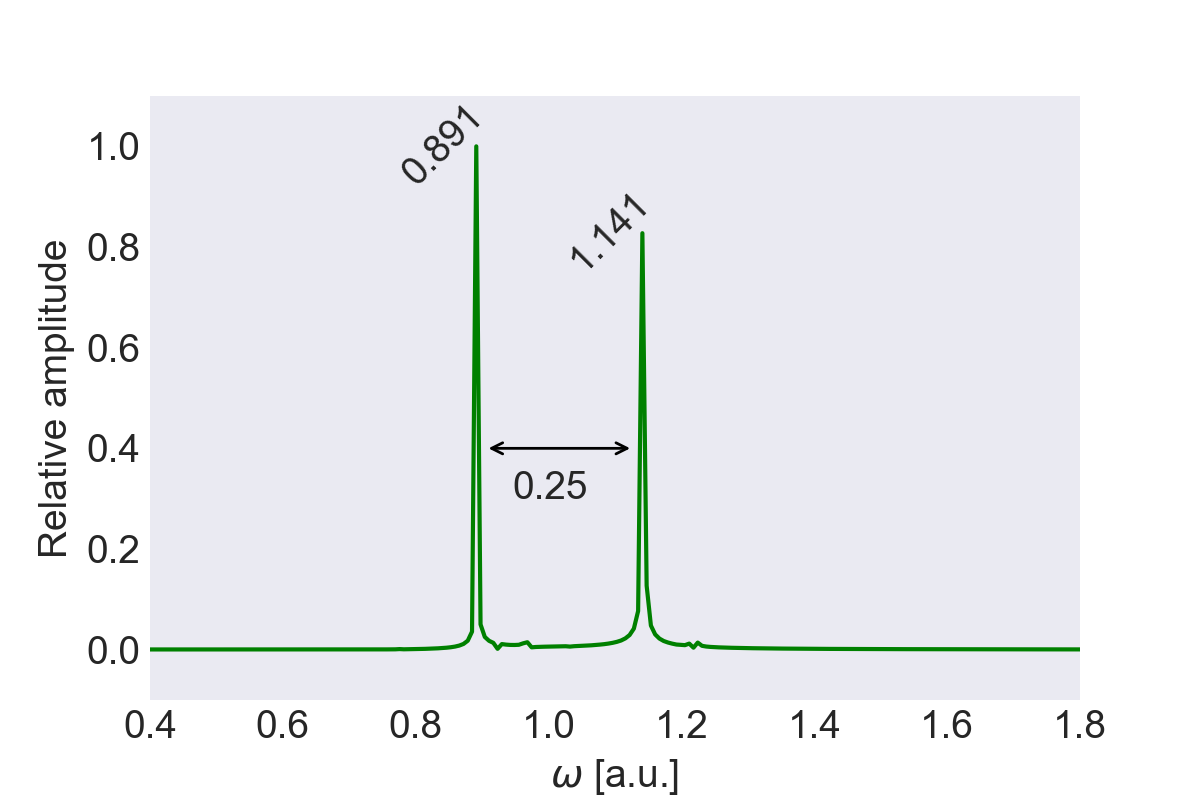
\includegraphics[width=0.75\textwidth]
        {results/figures/B_field/n=2/b_spectrum_omc025.png}
    \caption{Dipole spectrum of a quantum dot with $n=2$ electrons
    subjected to a magnetic field with Larmor frequency $\omega_c=0.25$.} 
    \label{fig:b_n2_omc025}
\end{figure}

\begin{figure}
    \centering    
    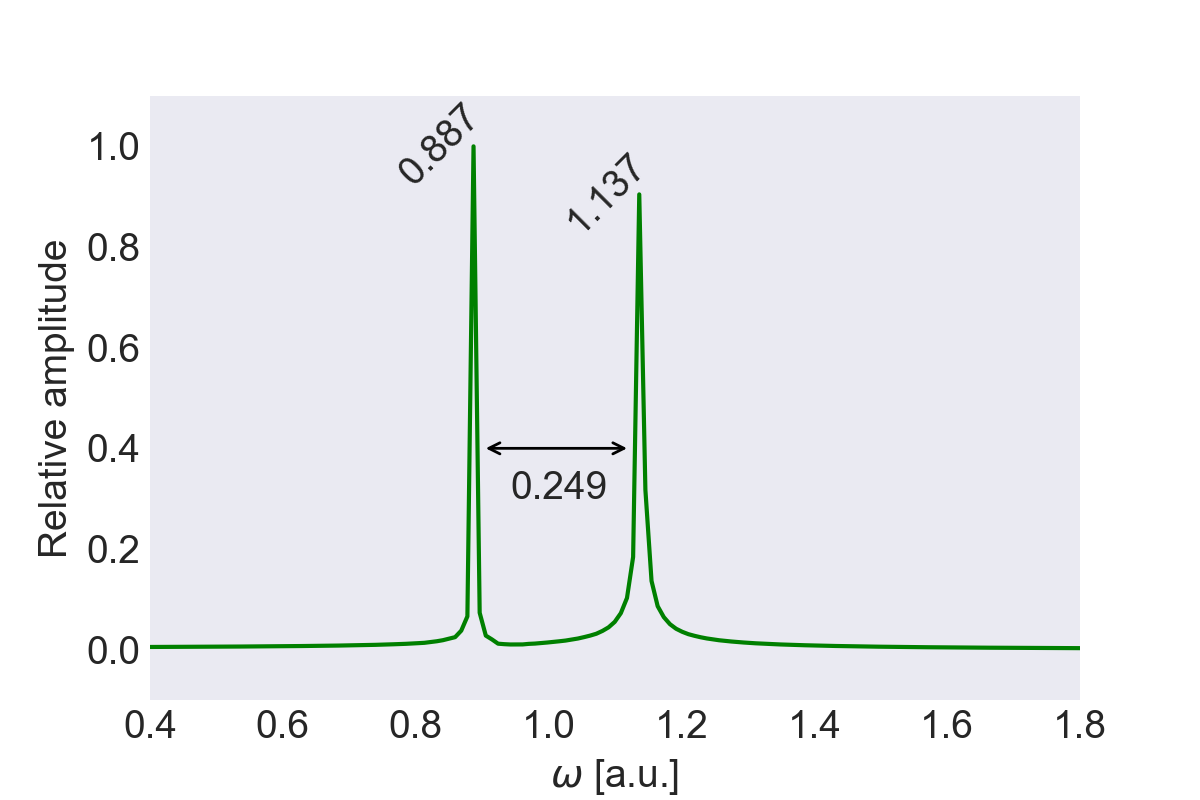
\includegraphics[width=0.75\textwidth]
        {results/figures/B_field/n=4/b_spectrum_n=4_omc=025.png}
    \caption{Dipole spectrum of a quantum dot with $n=2$ electrons
    subjected to a magnetic field with Larmor frequency $\omega_c=0.25$.}
    \label{fig:b_n4_omc025}
\end{figure}


    \part{Conclusion}

        \chapter{Summary Remarks}

The aim of this thesis was to develop and test numerical methods for 
soling the time-dependent Schrödinger equation. In particular, we 
wanted to develop the Orbital Adaptive Time-Dependent Coupled Cluster 
(OATDCC) method introduced by \citeauthor{kvaal2012ab}\cite{kvaal2012ab}.

We can with confidence say that this endevour has been succesful.
We have implemented both 
a time-depedent Coupled Cluster Singles Doubles (TDCCSD) solver with 
static orbitals and an \emph{Orbital Adaptive} Time-Dependent Coupled Cluster 
Doubles (OATDCCD) solver, as well as several quantum systems and an interface 
to quantum chemistry software which enables extraction of further basis sets.
The resulting product is two modules for python; \lstinline{quantum_systems} 
and \lstinline{coupled_cluster}.

With these methods we have have managed to produce 
many results found in the existing literature on time-dependent ab initio 
many-body solvers. This includes a reproduction of the instantaneous dipole 
of $H_2$ from \citeauthor{li2005time}\cite{li2005time}, the time-dependent 
ground state probability of a one-dimensional quantum dot from 
\citeauthor{Zanghellini04}\cite{Zanghellini04}, the dipole spectrum of 
helium from \citeauthor{pedersen2019symplectic}\cite{pedersen2019symplectic}
and the ionisation of a one-dimensional model of beryllium from 
\citeauthor{miyagi2013time}\cite{miyagi2013time}.

We have been able to compute the time-development 
of a relatively high number of particles, up to $n=12$ electrons in one- and
two-dimensional quantum dots. This stands as a testimony to the robustment 
of our implementations. For ever-increasing basis set size we have produced 
time-dependent results that converge, adding to the confidence in the results.
The results relating to the quantum dots are in accordance with the 
results one would expect from theory. Specifically, in both one-dimensional 
and two-dimensional quantum dots we have shown that the harmonic potential 
theorem\cite{kohn1961cyclotron} holds - the dipole spectrum of quantum 
dots consists of only one line consistent with the oscillator frequency in 
ordinary harmonic quantum dots. For the two-dimensional double dot system,
we also see only one spectral line, but a shift in frequency. By adding a homogenous,
static magnetic field to the quantum dot, we see a split in the dipole spectrum 
resulting in two spectral lines at a distance equal to the Larmor frequency of 
the applied magnetic field.

In assesment of the time-dependent coupled cluster method with static orbitals,
we found that the solver struggles to correctly represent the current state if 
the system progresses too far away from the inital reference state. As such the 
method is not a method that one can trusts blindly, as the method returns
inaccurate results in these sitations. This phenomenon manisfests most clearly as 
non-sensical ground state overlap values, but also as exceedingly high amplitude 
values. The orbital-adaptive solver will remedy this problem, but has a drawback 
in that it cannot feasibly produce inner products of two states in time, and therefore 
is unable to compute time-dependent ground state probabilities.

This study, with the addition the the study by \citeauthor{islandwind2019}\cite{islandwind2019},
have only scratched the surface with regards to the cornucopia of results that our 
code base is able to produce. The reason for this is for the most part attributed to 
the time spent in development and the amount in wall clock time necessary to 
produce the results herein. A challenge with time-dependent studies is the 
impossibility of true parallelisation, as time step $t_n$ will always depend 
on $t_{n-1}$.

\section{Further Studies}

By study of the results we have produced, we think that a comparison study 
of the method with static orbitals and the one with adaptive orbitals is warranted.
One would assume that the two methods yields identical results within a reasonable 
upper limit in basis set size, but under what conditions do we get close to this
limit? We can for instance imagine that the orbital-adaptive scheme yields equivalent
results compared to the static-orbital method for a lower number of spin-orbitals,
because of the automatic adaption to the current state that an orbital adaption 
provides.

As of now, the apparatus we have manufactured can easily be used to model 
the time-dependent behaviour of additional systems. In fact, one could even 
easily argue that the complete investigation of the systems we have implemented 
ourselves in \lstinline{quantum_dots} is far from over. We have already begun
the implementation of a smoother two-dimensional double well potential, and 
improved and more interesting well potentials such as the double double dot 
from \citeauthor{nielsen2012configuration}\cite{nielsen2012configuration}. Another 
idea is the construction of potential that are not circular-symmetric.
That said, we regrattably only had time to study \emph{one} of the
\emph{five} potentials we have implemented for the one-dimensional quantum dot.
The addition of a three-dimensional quantum dot system would also be essential 
in any further studies. Hre, the integral elements provided by
\citeauthor{vorrath2003electronic}\cite{vorrath2003electronic} would be useful.

We would also like to see the addition of more exotic terms to the Hamiltian in the 
quantum dot systems. We think it would not be too difficult to add a spin-operator 
terms $\hat{S}_x$, $\hat{S}_y$, $\hat{S}_z$, spin-spin coupling terms
$\hat{S}\cdot\hat{S}$, and spin-orbit
coupling terms $\hat{J}^2$, $\hat{L}\cdot\hat{S}$. We belive that these would provide 
very interesting results and enables us to model resplendent physical effects. We are 
confident that hte 
mere addition of a $\hat{S}_z$ operator would enable us to see Zeeman splitting in 
the dipole spectrum of quantum dots, for instance. Eventually, one could hope to 
implement much more complicated operators, such as quantum logic gates, with the 
hope of consequent simulation of quantum circuitry.

Richer physics can also be modelled by a the implementation of higher order 
multi-pole terms for the oscillating laser field. Moving beyond the allowed transitions
dictated by the dipole approximation could yield some interesting results.
 

    \part{Appendices}
    \appendix

        \chapter{Quantum Dot Results}

\vfill
\pagebreak

\section{One Dimension}
\label{app:1d_qd}

\subsection*{Four electrons}

\begin{figure}[h]
    \centering
    \makebox[\textwidth][c]{
    \begin{minipage}{0.6\textwidth}
        \centering
        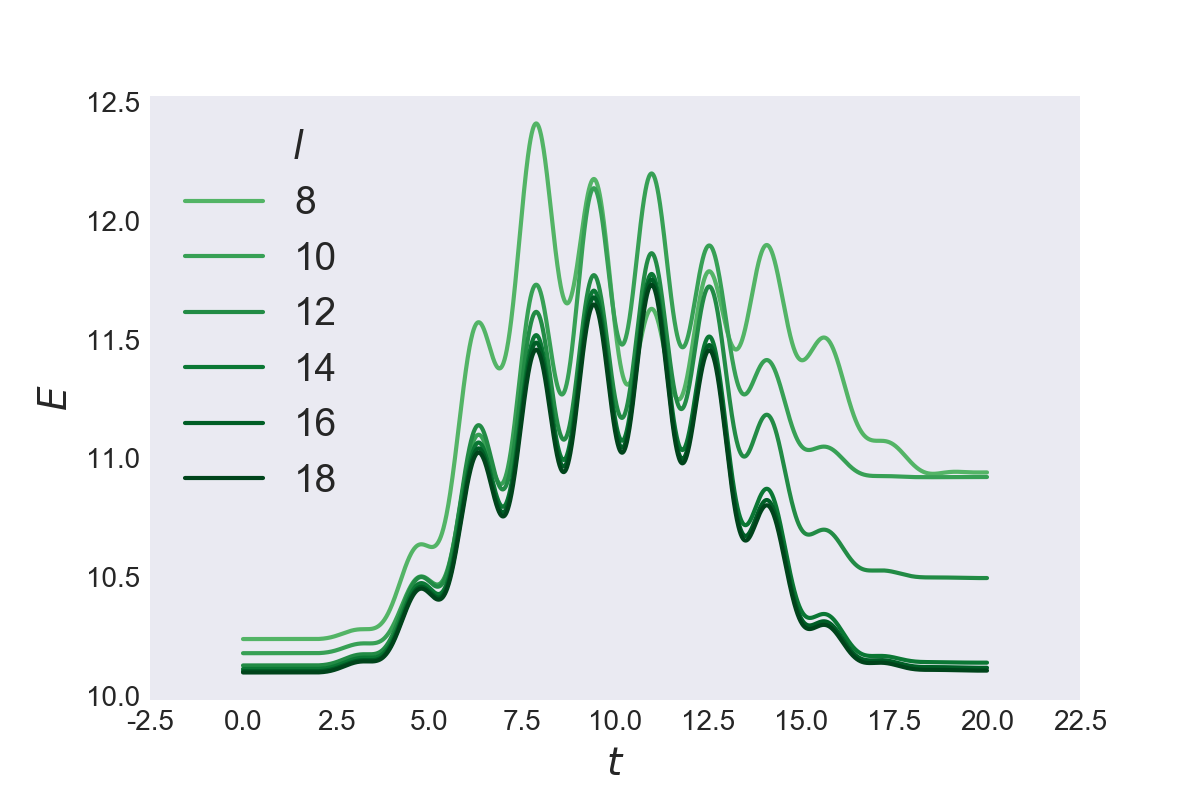
\includegraphics[width=\textwidth]{results/figures/1D/n=4energy.png}
    \end{minipage}\hfill 
    \begin{minipage}{0.6\textwidth}
        \centering 
        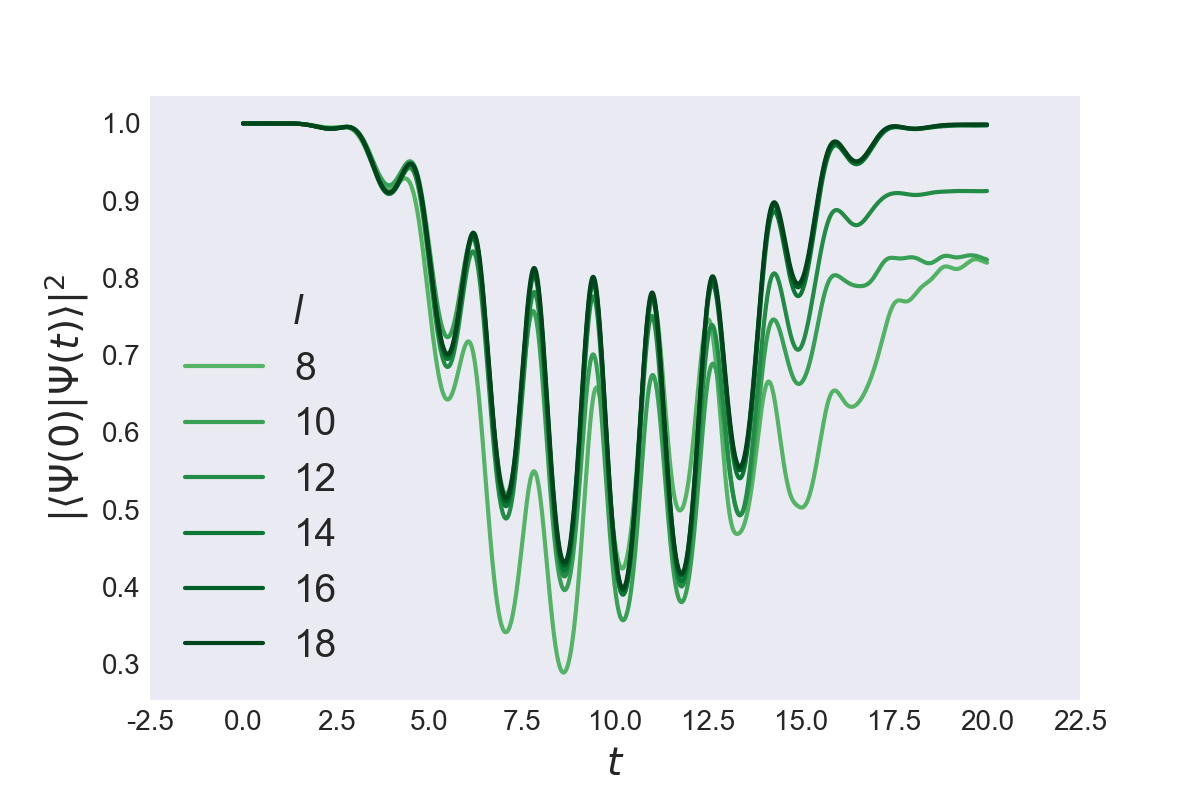
\includegraphics[width=\textwidth]{results/figures/1D/n=4overlap.png}
    \end{minipage}
    }
    \caption{Time-dependent energy (left) and ground state probability (right)
        of a one-dimensional harmonic oscillator with $\Omega=1$
        and $n=4$ electrons under the influence of a oscillating electric field 
        of frequency $\omega = 2 \Omega = 2$ and field strength $\vb{E}_\text{max}=1$,
        for different number of spin-orbitals $l=\{8,10,12,14,16,18\}$.
    }
    \label{fig:1d_n4_qd}
\end{figure}

\begin{figure}[!h]
    \centering
    \makebox[\textwidth][c]{
    \begin{minipage}{0.6\textwidth}
        \centering
        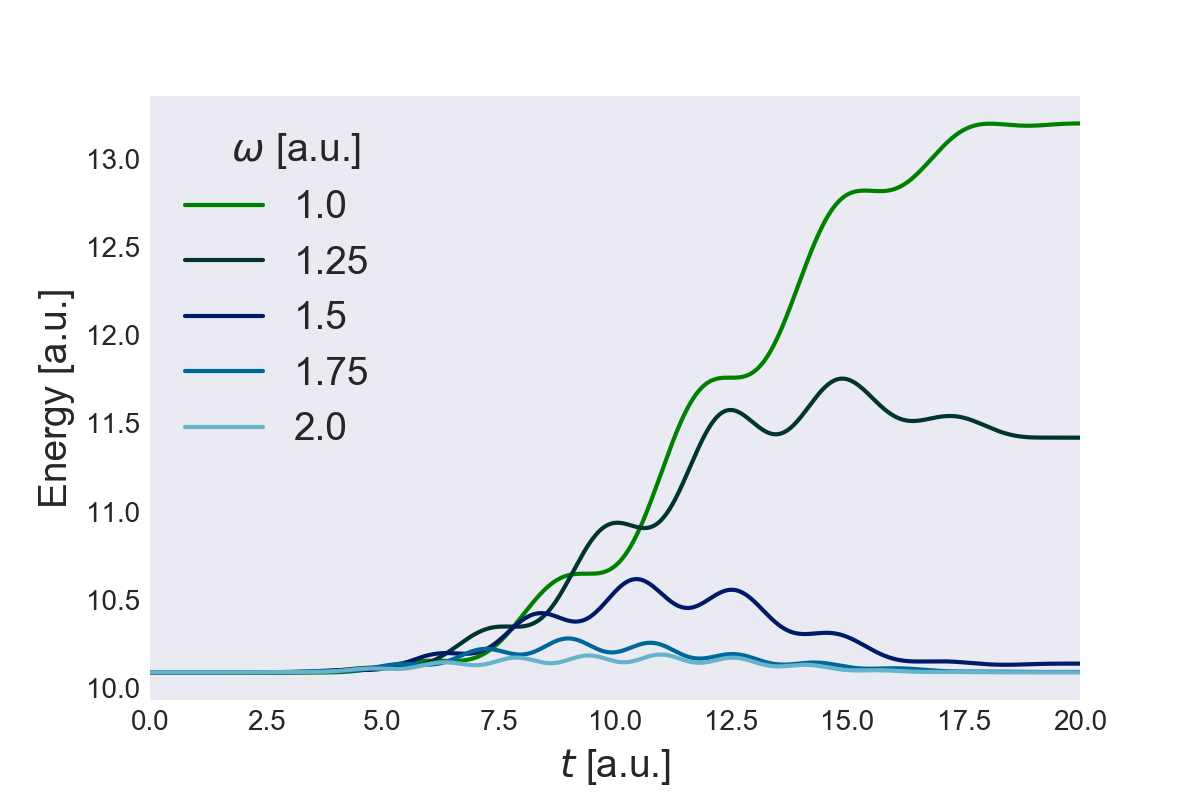
\includegraphics[width=\textwidth]{results/figures/1D/n4_resonance_energy.png}
    \end{minipage}\hfill 
    \begin{minipage}{0.6\textwidth}
        \centering 
        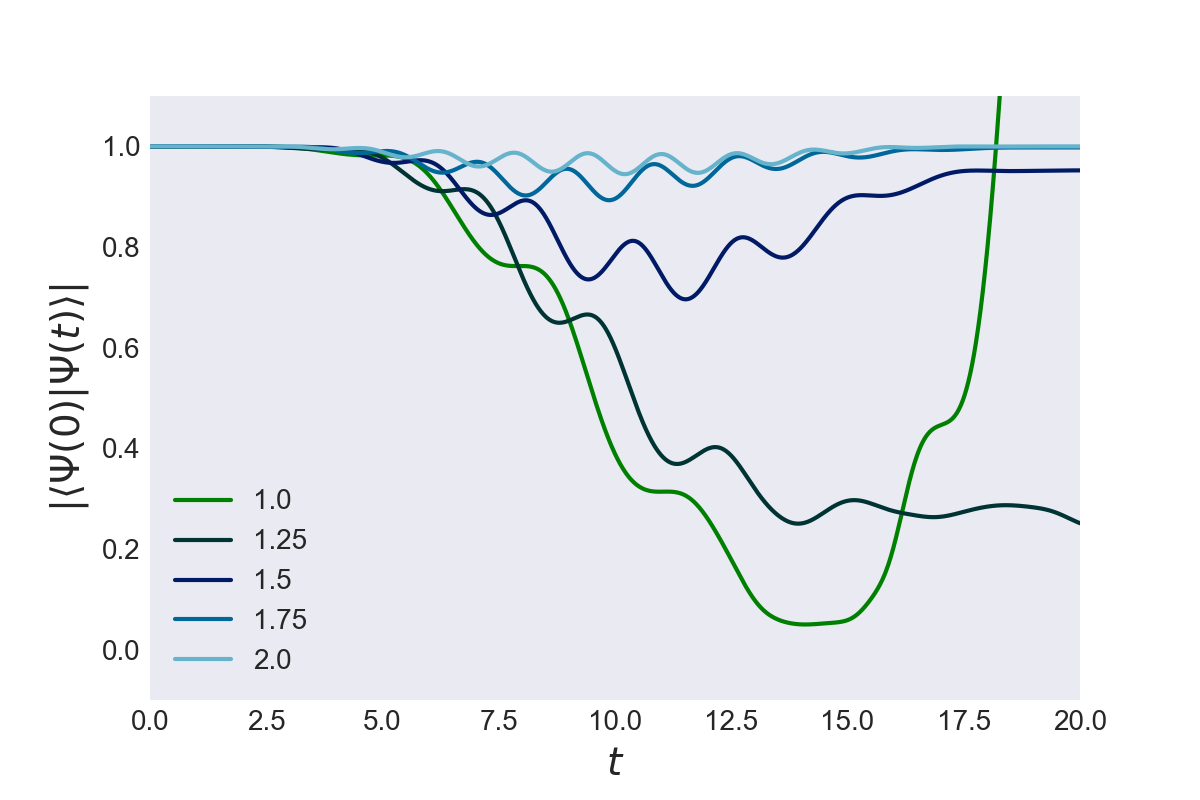
\includegraphics[width=\textwidth]{results/figures/1D/n4_resonance_overlap.png}
    \end{minipage}
    }
    \caption{Time-dependent energy (left) and ground state probability (right)
        of a one-dimensional harmonic oscillator with $\Omega=1$
        and $n=4$ electrons under the influence of a oscillating electric field 
        of different frequencies $\omega\in\{1.0, 1.25, 1.5, 1.75, 2.0\}$ with 
        maximum field strength $\vb{E}_\text{max}=0.25$ and $l=30$ 
        spin-orbitals.
    }
    \label{fig:1d_n4_qd_resonance}
\end{figure}

\vfill
\pagebreak

\subsection*{Six electrons}

\begin{figure}[!h]
    \centering
    \makebox[\textwidth][c]{
    \begin{minipage}{0.6\textwidth}
        \centering
        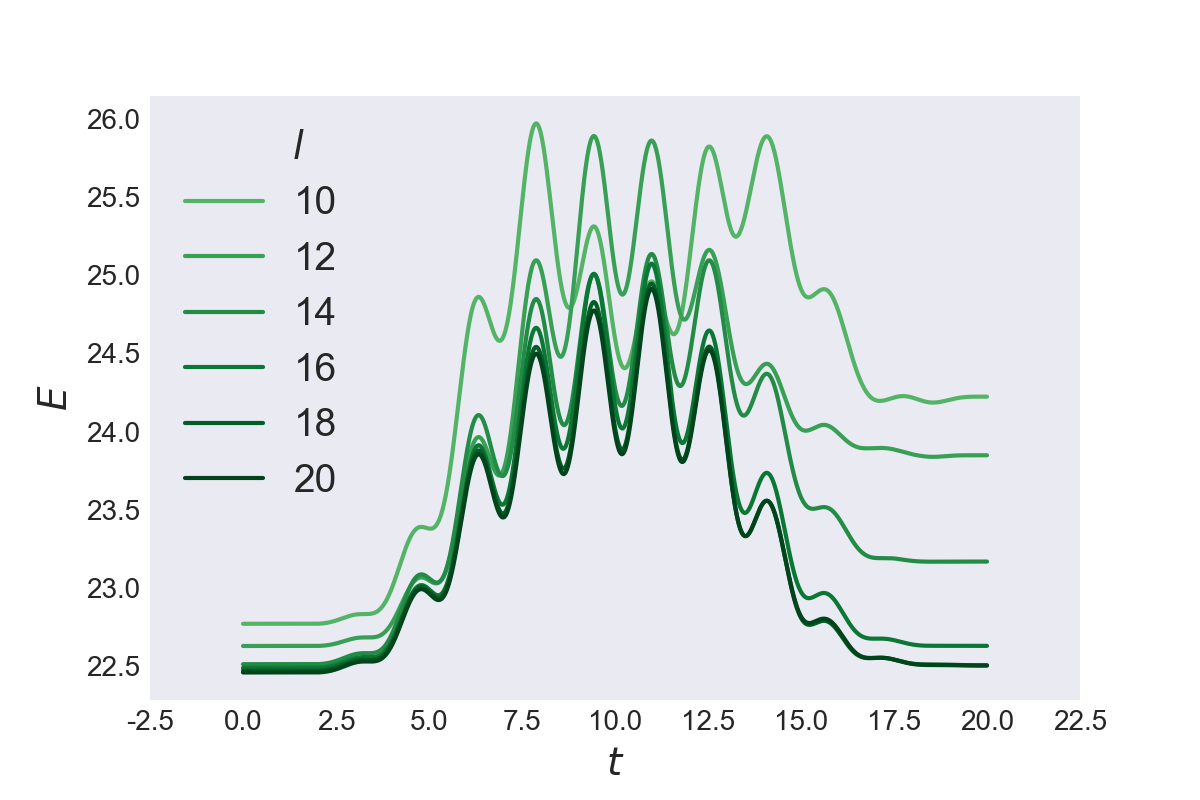
\includegraphics[width=\textwidth]{results/figures/1D/n=6energy.png}
    \end{minipage}\hfill 
    \begin{minipage}{0.6\textwidth}
        \centering 
        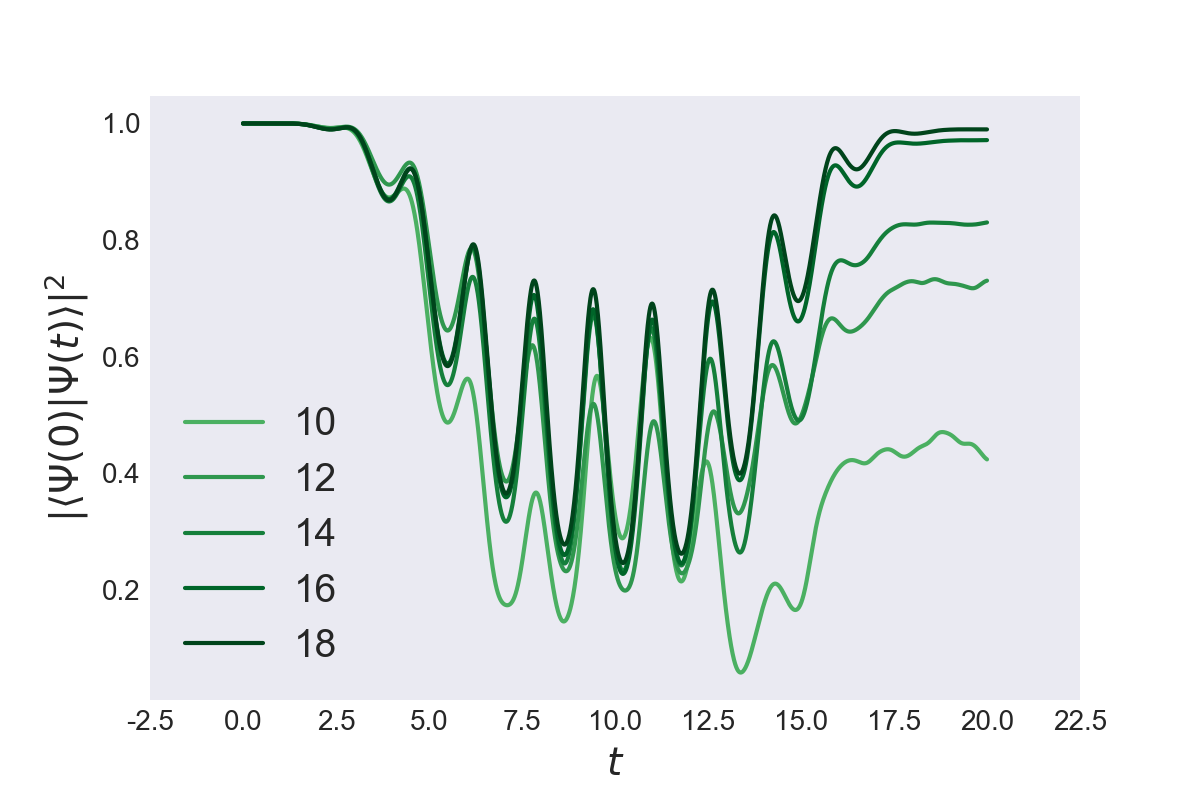
\includegraphics[width=\textwidth]{results/figures/1D/n=6overlap.png}
    \end{minipage}
    }
    \caption{Time-dependent energy (left) and ground state probability (right)
        of a one-dimensional harmonic oscillator with $\Omega=1$
        and $n=6$ electrons under the influence of a oscillating electric field 
        of frequency $\omega = 2 \Omega = 2$ and field strength $E_\text{max}=1$,
        for different number of spin-orbitals $l=\{10,12,14,16,18,20\}$.
    }
    \label{fig:1d_n6_qd}
\end{figure}

\begin{figure}[!h]
    \centering
    \makebox[\textwidth][c]{
    \begin{minipage}{0.6\textwidth}
        \centering
        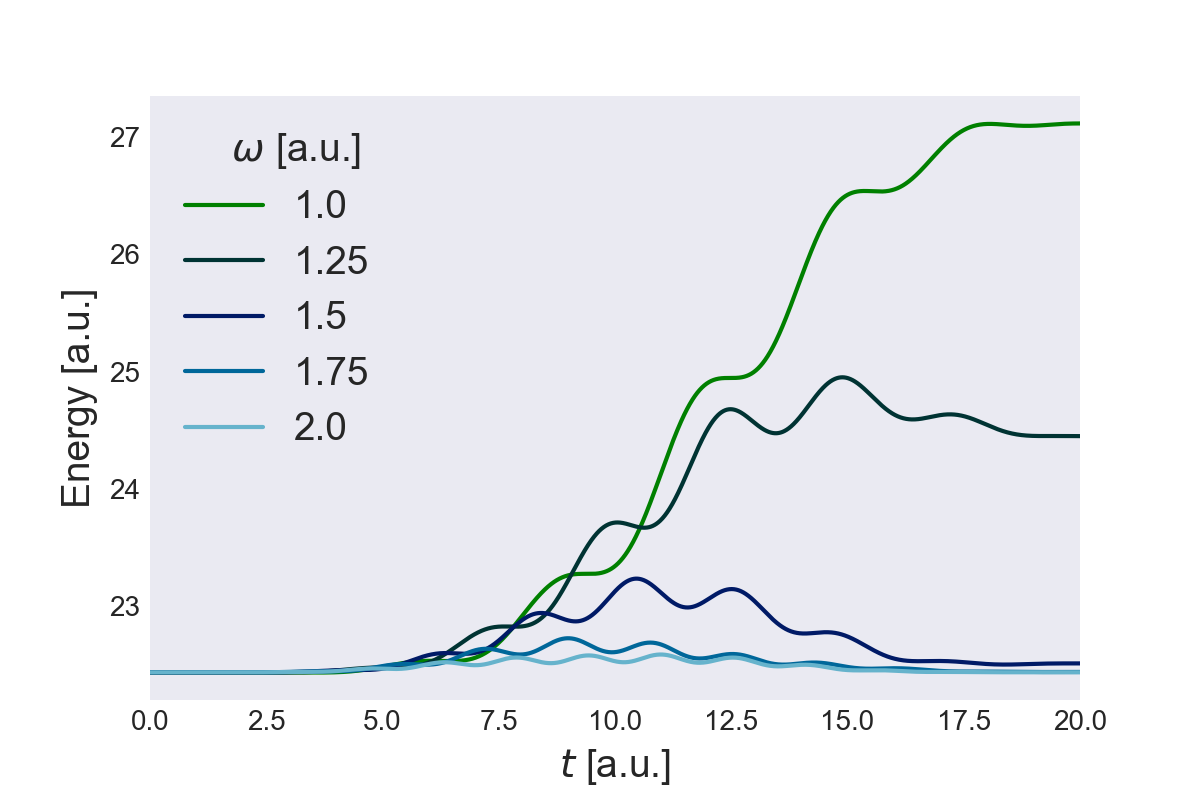
\includegraphics[width=\textwidth]{results/figures/1D/n6_resonance_energy.png}
    \end{minipage}\hfill 
    \begin{minipage}{0.6\textwidth}
        \centering 
        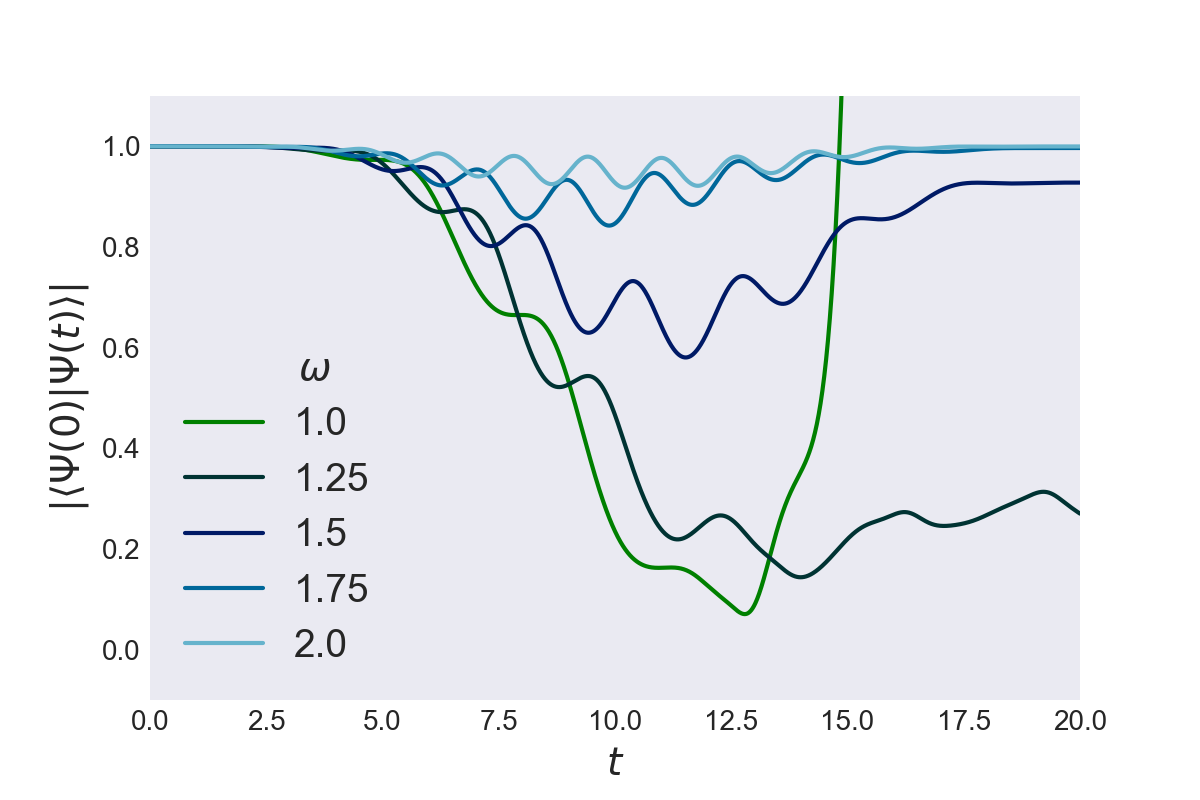
\includegraphics[width=\textwidth]{results/figures/1D/n6_resonance_overlap.png}
    \end{minipage}
    }
    \caption{Time-dependent energy (left) and ground state probability (right)
        of a one-dimensional harmonic oscillator with $\Omega=1$
        and $n=6$ electrons under the influence of a oscillating electric field 
        of different frequencies $\omega\in\{1.0, 1.25, 1.5, 1.75, 2.0\}$ with 
        maximum field strength $\vb{E}_\text{max}=0.25$ and $l=30$ 
        spin-orbitals.
    }
    \label{fig:1d_n6_qd_resonance}
\end{figure}

\vfill
\pagebreak

\subsection*{Eight electrons}

\begin{figure}[!h]
    \centering
    \makebox[\textwidth][c]{
    \begin{minipage}{0.6\textwidth}
        \centering
        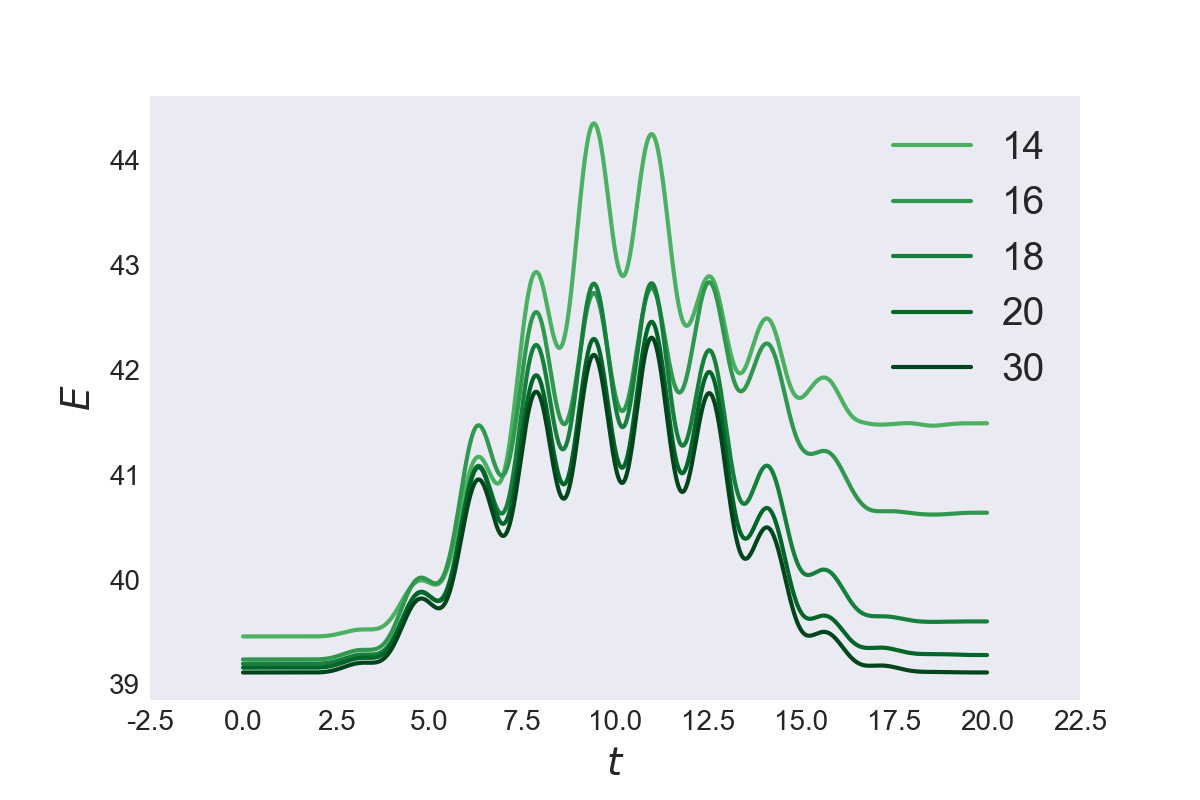
\includegraphics[width=\textwidth]{results/figures/1D/n=8energy.png}
    \end{minipage}\hfill 
    \begin{minipage}{0.6\textwidth}
        \centering 
        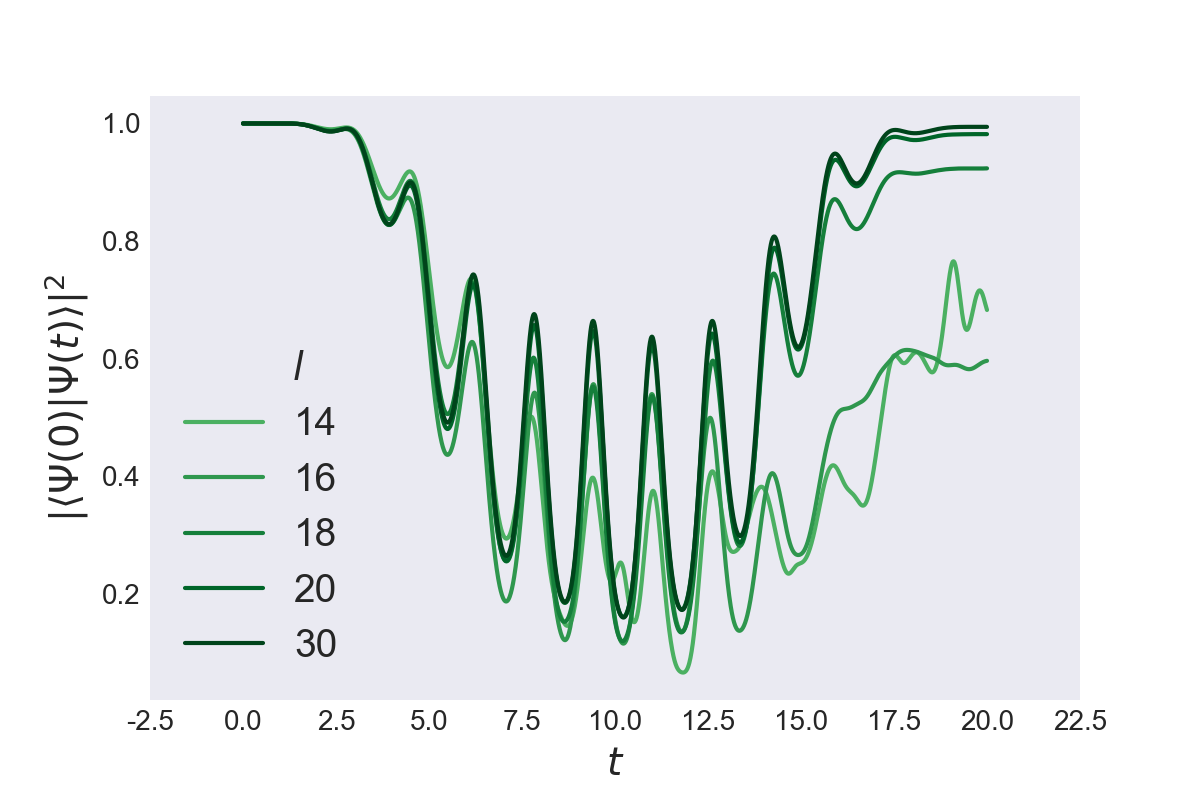
\includegraphics[width=\textwidth]{results/figures/1D/n=8overlap.png}
    \end{minipage}
    }
    \caption{Time-dependent energy (left) and ground state probability (right)
        of a one-dimensional harmonic oscillator with $\Omega=1$
        and $n=8$ electrons under the influence of a oscillating electric field 
        of frequency $\omega = 2 \Omega = 2$ and field strength $E_\text{max}=1$,
        for different number of spin-orbitals $l=\{14,16,18,20,30\}$.
    }
    \label{fig:1d_n8_qd}
\end{figure}

\begin{figure}[!h]
    \centering
    \makebox[\textwidth][c]{
    \begin{minipage}{0.6\textwidth}
        \centering
        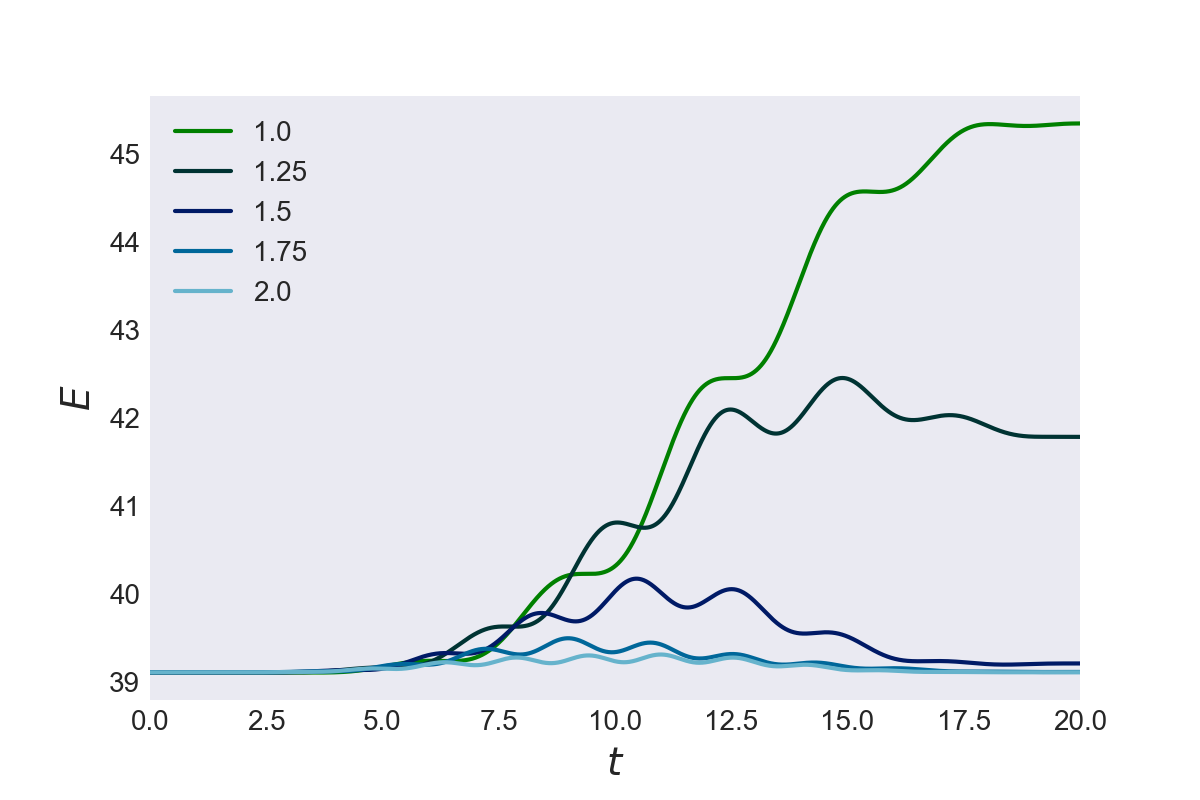
\includegraphics[width=\textwidth]{results/figures/1D/n8_resonance_energy.png}
    \end{minipage}\hfill 
    \begin{minipage}{0.6\textwidth}
        \centering 
        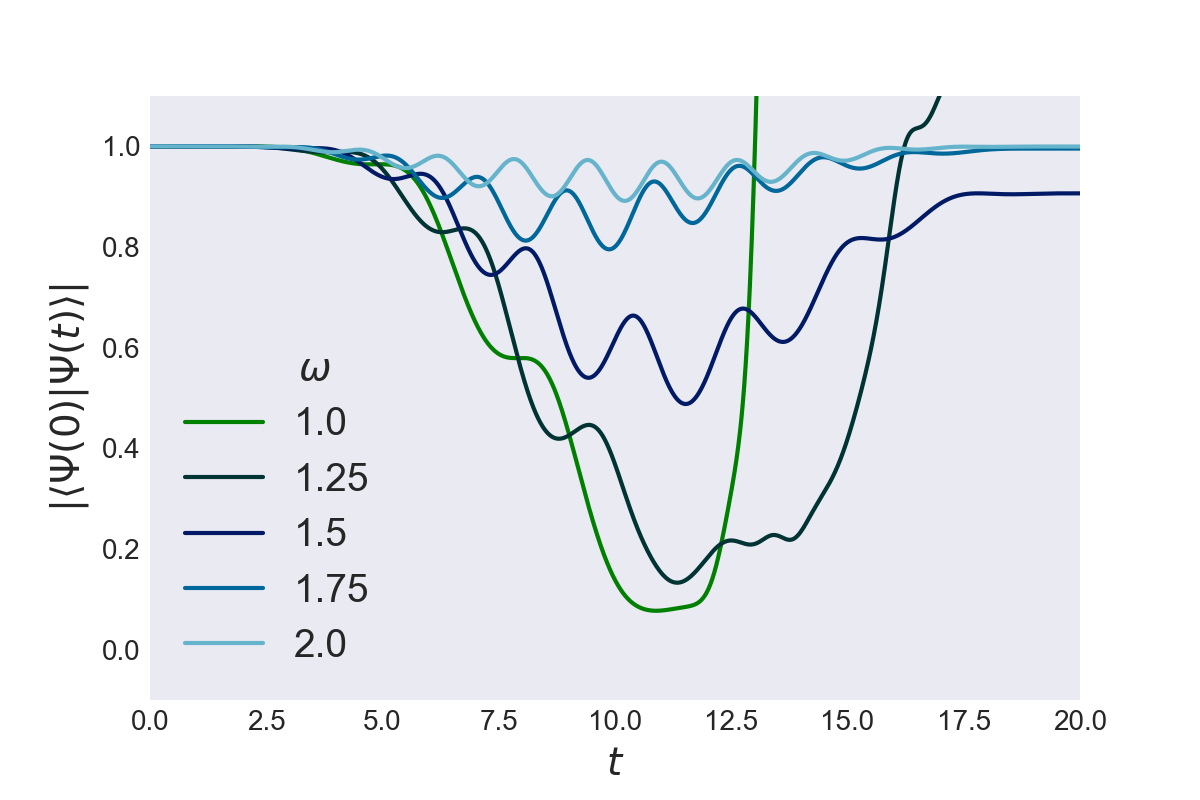
\includegraphics[width=\textwidth]{results/figures/1D/n8_resonance_overlap.png}
    \end{minipage}
    }
    \caption{Time-dependent energy (left) and ground state probability (right)
        of a one-dimensional harmonic oscillator with $\Omega=1$
        and $n=8$ electrons under the influence of a oscillating electric field 
        of different frequencies $\omega\in\{1.0, 1.25, 1.5, 1.75, 2.0\}$ with 
        maximum field strength $\vb{E}_\text{max}=0.25$ and $l=36$ 
        spin-orbitals.
    }
    \label{fig:1d_n8_qd_resonance}
\end{figure}

\vfill
\pagebreak

\subsection*{Ten electrons}

\begin{figure}[!h]
    \centering
    \makebox[\textwidth][c]{
    \begin{minipage}{0.6\textwidth}
        \centering
        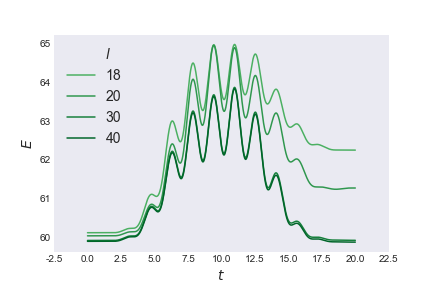
\includegraphics[width=\textwidth]{results/figures/1D/n=10energy.png}
    \end{minipage}\hfill 
    \begin{minipage}{0.6\textwidth}
        \centering 
        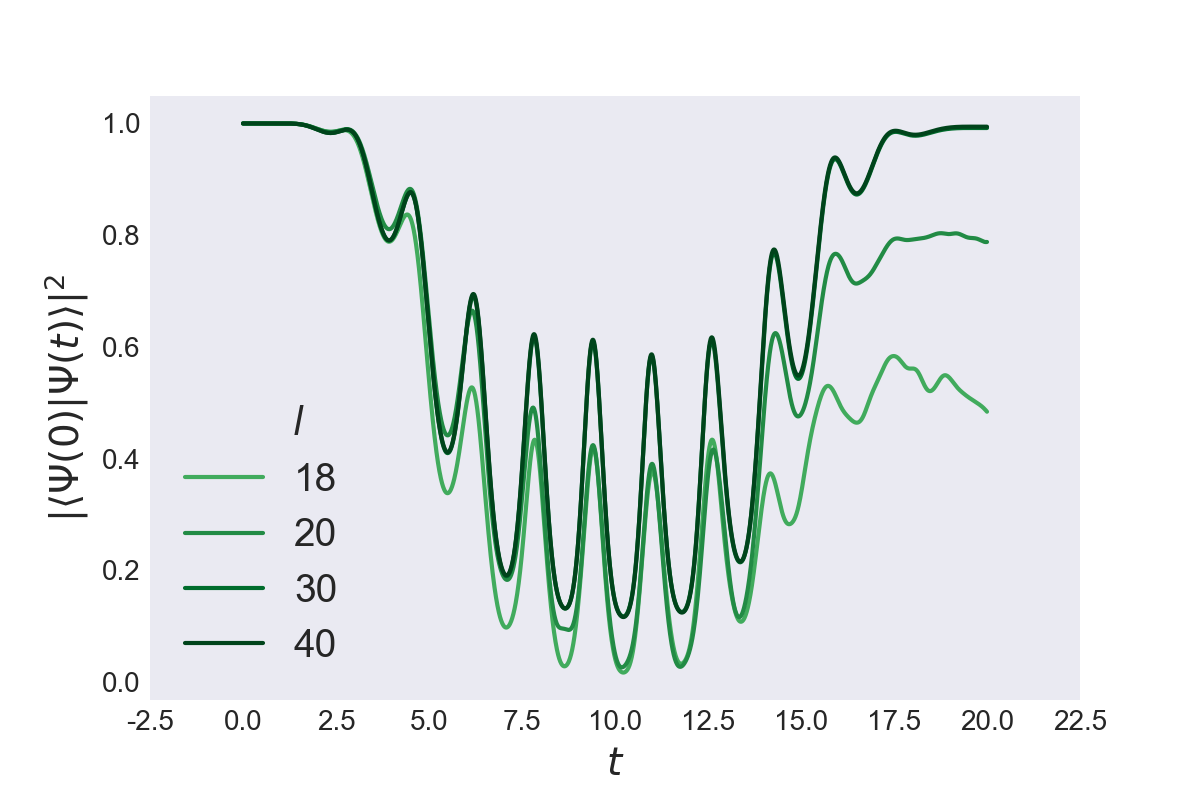
\includegraphics[width=\textwidth]{results/figures/1D/n=10overlap.png}
    \end{minipage}
    }
    \caption{Time-dependent energy (left) and ground state probability (right)
        of a one-dimensional harmonic oscillator with $\Omega=1$
        and $n=10$ electrons under the influence of a oscillating electric field 
        of frequency $\omega = 2 \Omega = 2$ and field strength $E_\text{max}=1$,
        for different number of spin-orbitals $l=\{18,20,30,40\}$.
    }
    \label{fig:1d_n10_qd}
\end{figure}

\begin{figure}[!h]
    \centering
    \makebox[\textwidth][c]{
    \begin{minipage}{0.6\textwidth}
        \centering
        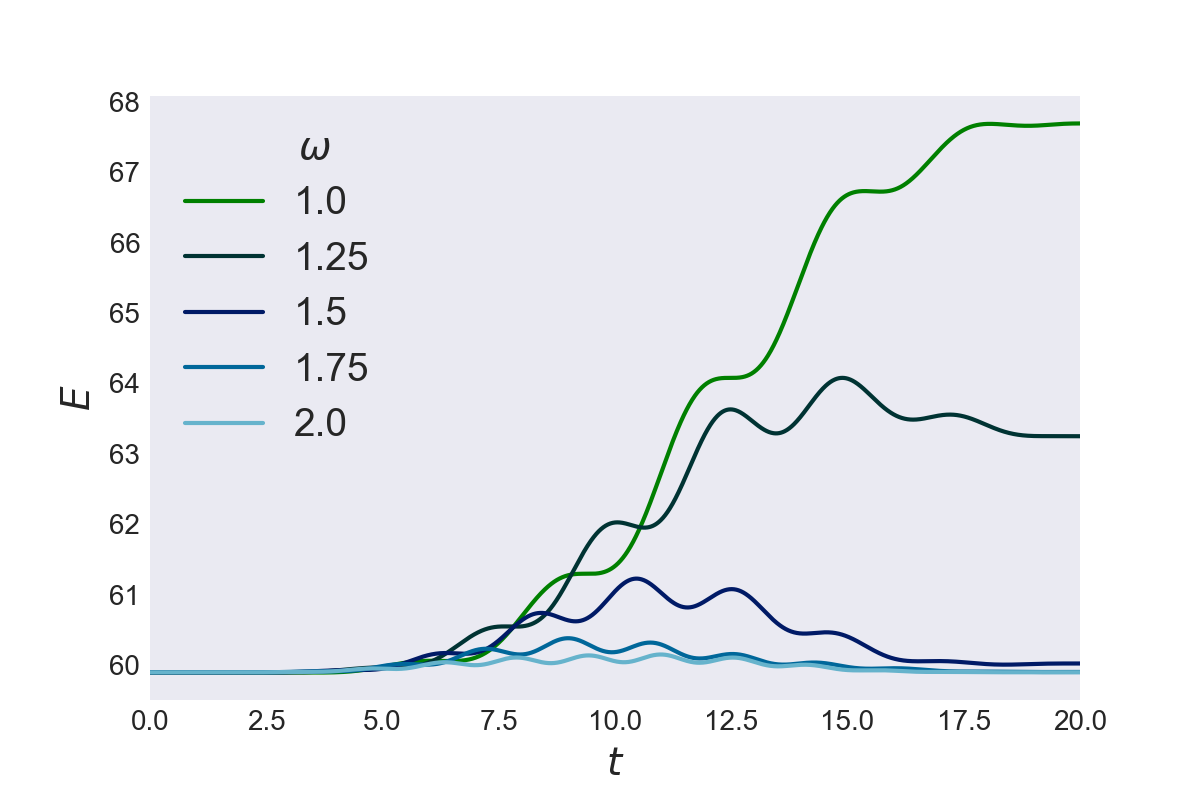
\includegraphics[width=\textwidth]{results/figures/1D/n10_resonance_energy.png}
    \end{minipage}\hfill 
    \begin{minipage}{0.6\textwidth}
        \centering 
        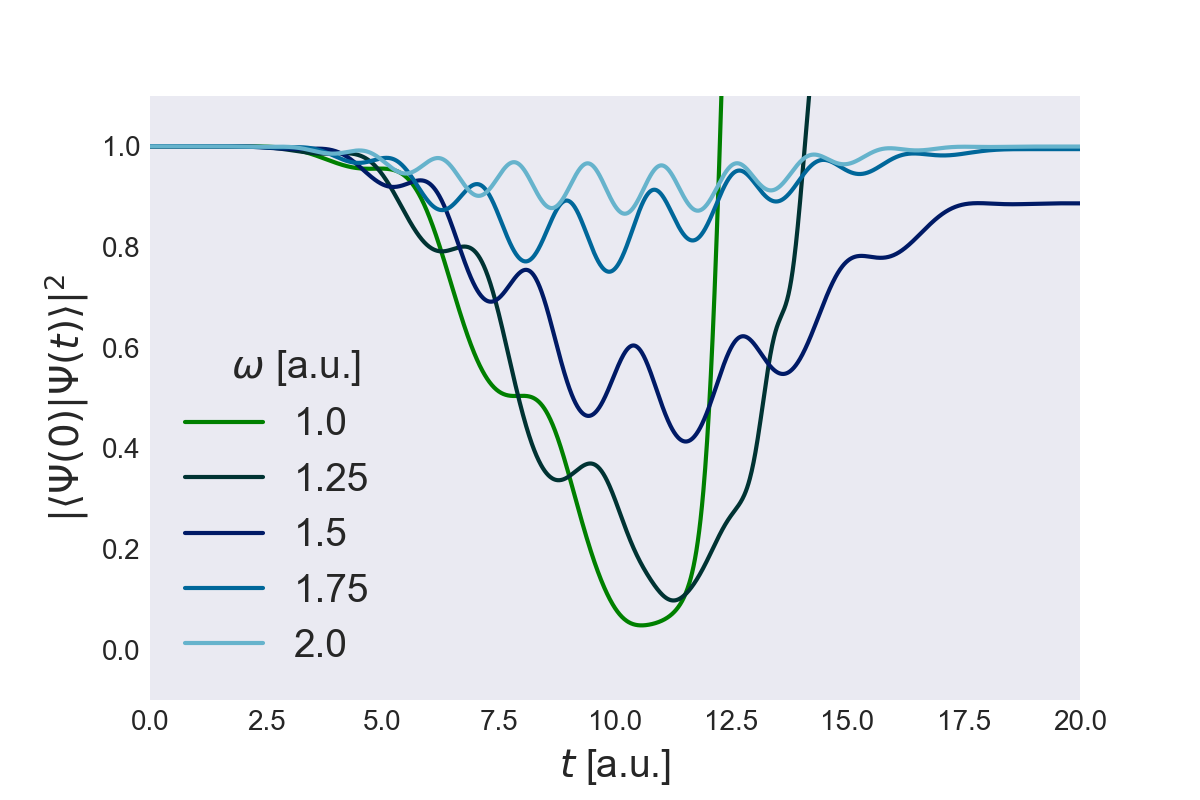
\includegraphics[width=\textwidth]{results/figures/1D/n10_resonance_overlap.png}
    \end{minipage}
    }
    \caption{Time-dependent energy (left) and ground state probability (right)
        of a one-dimensional harmonic oscillator with $\Omega=1$
        and $n=8$ electrons under the influence of a oscillating electric field 
        of different frequencies $\omega\in\{1.0, 1.25, 1.5, 1.75, 2.0\}$ with 
        maximum field strength $\vb{E}_\text{max}=0.25$ and $l=40$ 
        spin-orbitals.
    }
    \label{fig:1d_n10_qd_resonance}
\end{figure}

\vfill
\pagebreak

\subsection*{Twelve electrons}

\begin{figure}[!h]
    \centering
    \makebox[\textwidth][c]{
    \begin{minipage}{0.6\textwidth}
        \centering
        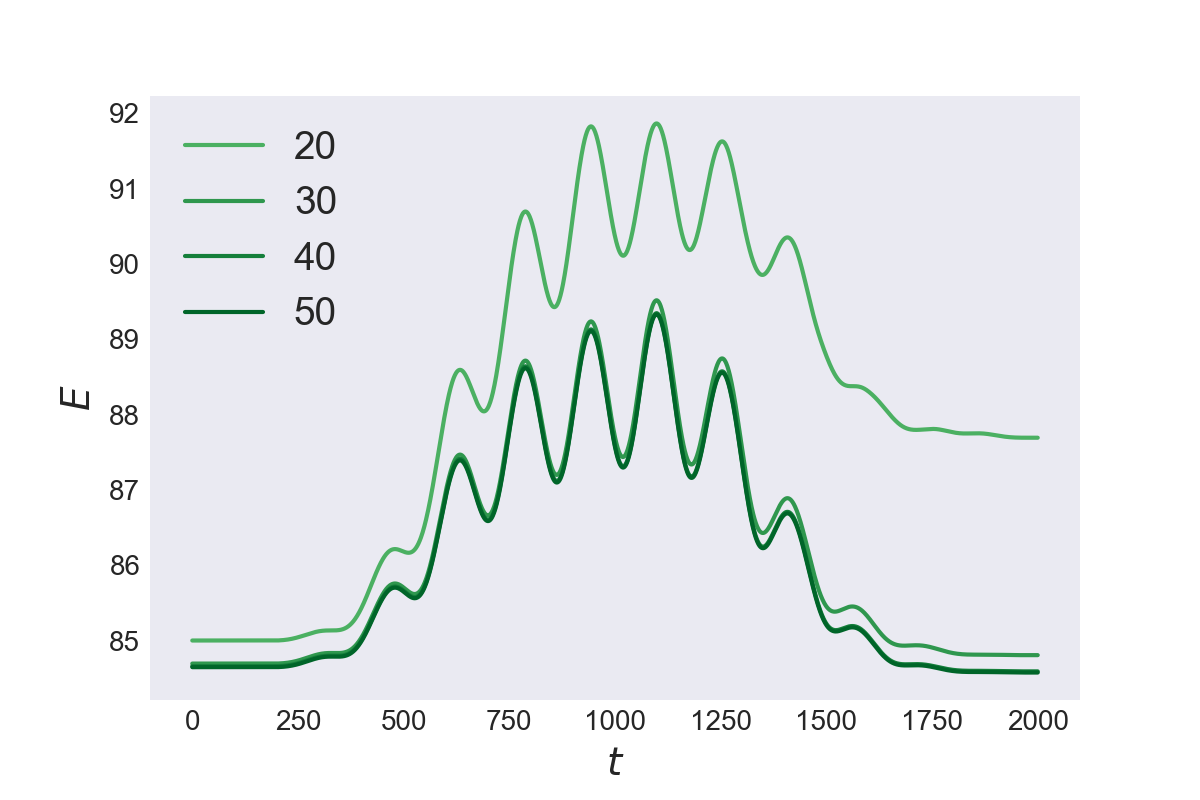
\includegraphics[width=\textwidth]{results/figures/1D/n=12energy.png}
    \end{minipage}\hfill 
    \begin{minipage}{0.6\textwidth}
        \centering 
        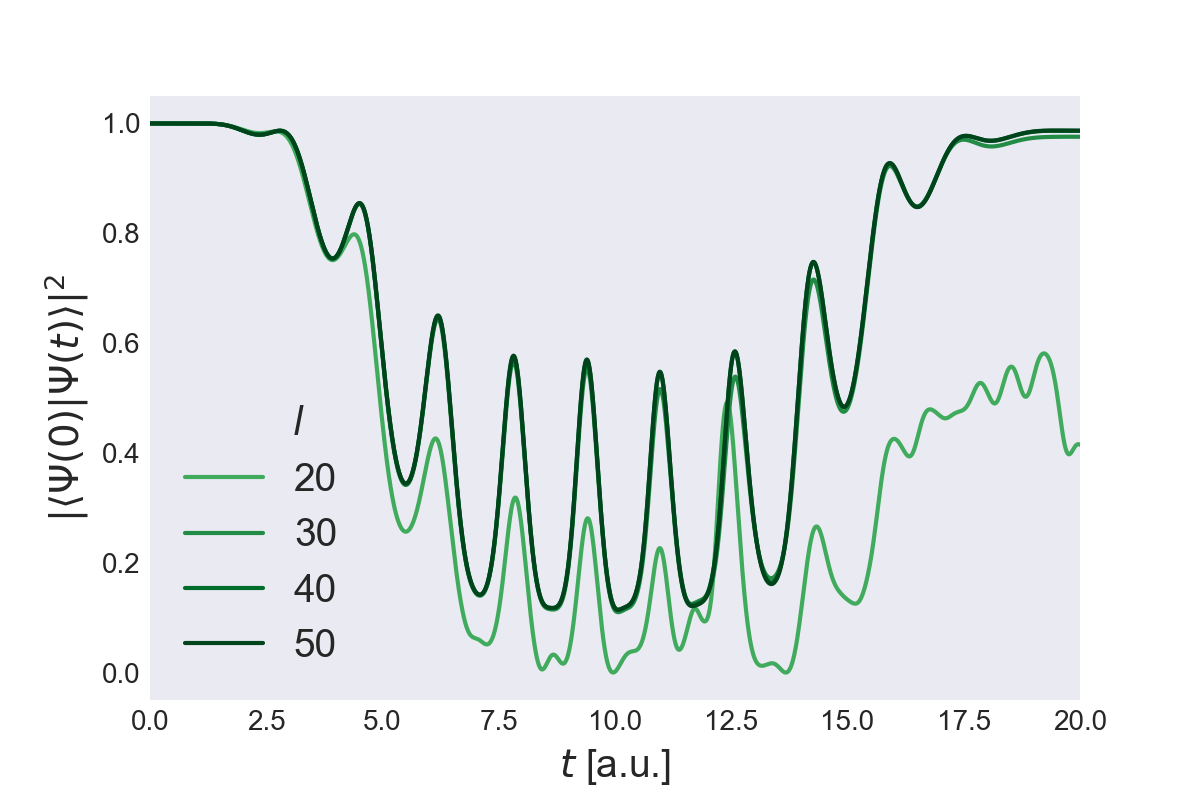
\includegraphics[width=\textwidth]{results/figures/1D/n=12overlap.png}
    \end{minipage}
    }
    \caption{Time-dependent energy (left) and ground state probability (right)
        of a one-dimensional harmonic oscillator with $\Omega=1$
        and $n=12$ electrons under the influence of a oscillating electric field 
        of frequency $\omega = 2 \Omega = 2$ and field strength $E_\text{max}=1$,
        for different number of spin-orbitals $l=\{20,30,40,50\}$.
    }
    \label{fig:1d_n12_qd}
\end{figure}

\vfill
\pagebreak


\section{Two Dimensions}
\label{app:supp_2d_qd_results}

\subsection*{Two electrons}

\begin{figure}[!h]
    \centering
    \makebox[\textwidth][c]{
    \begin{minipage}{0.6\textwidth}
        \centering
        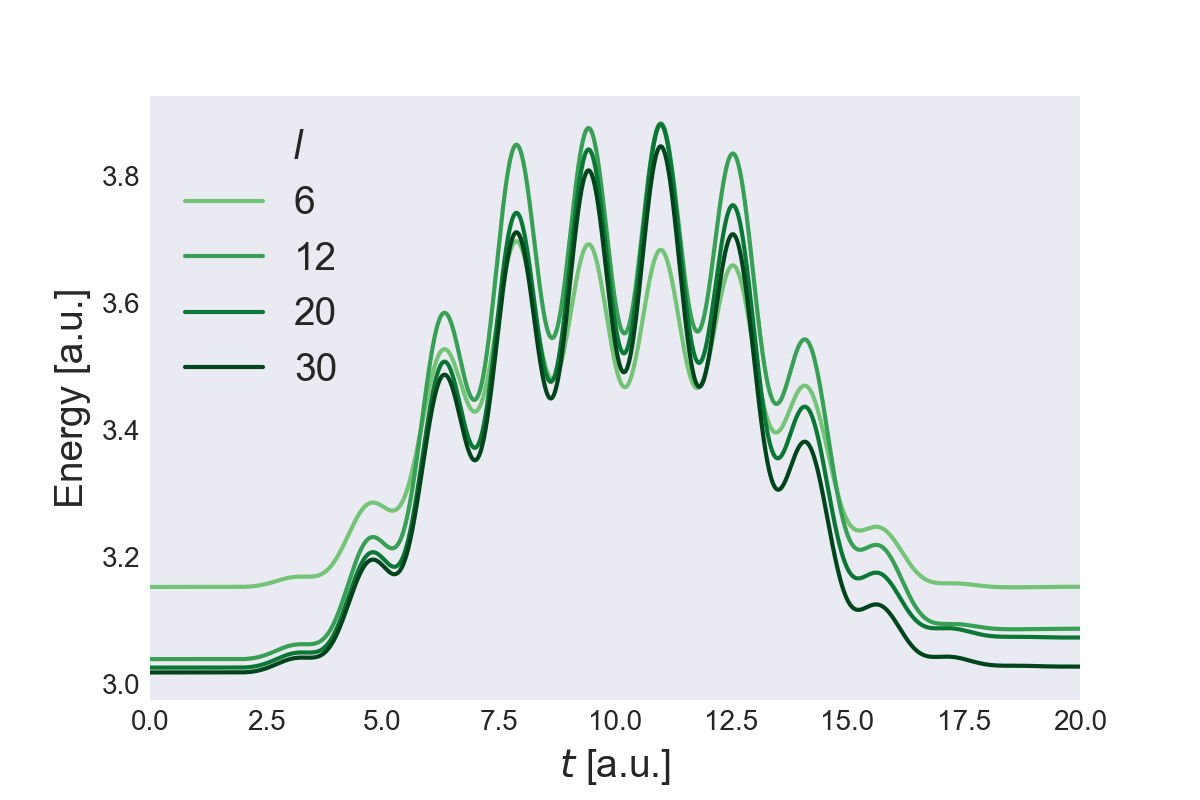
\includegraphics[width=\textwidth]{results/figures/2D/n2_energy.png}
    \end{minipage}\hfill 
    \begin{minipage}{0.6\textwidth}
        \centering 
        \includegraphics[width=\textwidth]{results/figures/2D/n2_overlap.png}
    \end{minipage}
    }
    \caption{Time-dependent energy (left) and ground state probability (right)
        of a two-dimensional harmonic oscillator with $\Omega=1$
        and $n=2$ electrons under the influence of a oscillating electric field 
        of frequency $\omega = 2 \Omega = 2$ and field strength $E_\text{max}=1$,
        for different number of spin-orbitals $l=\{6,12,20,30\}$.
    }
    \label{fig:2d_n2_qd}
\end{figure}


\subsection*{Six electrons}

\begin{figure}[!h]
    \centering
    \makebox[\textwidth][c]{
    \begin{minipage}{0.6\textwidth}
        \centering
        \includegraphics[width=\textwidth]{results/figures/2D/n6_energy.png}
    \end{minipage}\hfill 
    \begin{minipage}{0.6\textwidth}
        \centering 
        \includegraphics[width=\textwidth]{results/figures/2D/n6_overlap.png}
    \end{minipage}
    }
    \caption{Time-dependent energy (left) and ground state probability (right)
        of a two-dimensional harmonic oscillator with $\Omega=1$
        and $n=6$ electrons under the influence of a oscillating electric field 
        of frequency $\omega = 2 \Omega = 2$ and field strength $E_\text{max}=1$,
        for different number of spin-orbitals $l=\{6,12,20,30\}$.
    }
    \label{fig:2d_n6_qd}
\end{figure}

        \chapter{Coupled Cluster}

\section{CC and CI correspondence}
\label{app:cc_vs_ci}

Monkhorst\cite{monkhorst1977calculation} gives a general formuala for transferring 
back and forth between Coupled Cluster (CC) operators $\hat{T}_m$ and
Configuration Interaction (CI) operators $\hat{C}_m$,
\begin{equation}
    \hat{C}_m = \sum_{k}^m\frac{1}{k!}\sum_{|m_\mu|}
        \delta(m_1 + m_2 + \dots + m_k, m) \prod_{\mu=1}^k\hat{T}_{m_\mu},
\end{equation}
where the second sum is over all sets of $k$ $m_\mu$-values that sum up to $m$.
The first four of the terms are,
\begin{align}
    \hat{C}_1 &= \hat{T}_1 \\
    \hat{C}_2 &= \hat{T}_2 + \frac{1}{2} \hat{T}_1^2 \\
    \hat{C}_3 &= \hat{T}_3 + \hat{T}_1\hat{T}_2 + \frac{1}{3!} T_1^3 \\
    \hat{C}_4 &= \hat{T}_4 + \frac{1}{2}\hat{T}_2
        + \frac{1}{2}\hat{T}_2\hat{T}_1^2 + \frac{1}{4!}\hat{T}_1^4.
\end{align}
For the CCSD and CISDTQ wavfunctions we have,
\begin{gather}
    \ket{\Psi_{\text{CCSD}}} = \left(
        1 + \hat{T}_1 + \frac{1}{2}\hat{T}_1^2 + \frac{1}{3!}\hat{T}_1^3 
        + \hat{T}_2 + \frac{1}{2}\hat{T}_2^2 + \frac{1}{4!}\hat{T}_1^4 
        + \hat{T}_1\hat{T}_2 
    \right) \ket{\Phi_0} \\
    \ket{\Psi_{\text{CISDTQ}}} = \left(
        1 + \hat{C}_1 + \hat{C}_2  + \hat{C}_3 + \hat{C}_4
    \right)\ket{\Phi_0}
\end{gather}
which provides us with a relation between the two,
\begin{equation}
    \ket{\Psi_{\text{CCSD}}} 
        = \ket{\Psi_{\text{CISDTQ}}} - (\hat{T}_3 + \hat{T}_4)\ket{\Phi_0}.
\end{equation}
Moreover, for a system of $n=2$ particles, we have that
\begin{equation}
    \ket{\Psi_{\text{CCSD}}} = \ket{\Psi_{\text{CISD}}}.
\end{equation}


\chapter{Slater-Condon Rules}

% This stuff is mostly from page 60 and onwards in Shavitt and Bartlett

The Slater-Condon rules are ways to express integrals over operators in
terms of single-particle orbitals. Here is an outline of a proof for these
rules.

Consider first some Slater determinants,
\begin{gather}
    \ket{I} = \ket{i_1 i_2 \dots i_N} = 
        \hat{i}^\dagger_1 \hat{i}^\dagger_2 \dots \hat{i}^\dagger_N \ket{ } \\
    \ket{J} = \ket{j_1 j_2 \dots j_N} = 
        \hat{j}^\dagger_1 \hat{j}^\dagger_2 \dots \hat{j}^\dagger_N \ket{ }.
\end{gather}
To get started, we want to compute the inner product $\braket{I}{J}$ of these two Slater
determinants,
\begin{equation}
    \braket{I}{J} = \bra{ }\hat{i}_N \dots \hat{i}_2 \hat{i}_1 
    \hat{j}^\dagger_1 \hat{j}^\dagger_2 \dots \hat{j}^\dagger_N\ket{ }.
\end{equation}
In order to evaluate this expression, we move every annihilation operater $\hat{i}_p$
to the right. Starting with $\hat{i}_1$, for instance, we have two possible outcomes.
If there is no $\hat{j}_q$ that is the same as $\hat{i}_1$ we get
\begin{equation}
    \braket{I}{J} = \bra{ }\hat{i}_N \dots \hat{i}_2  
    \hat{j}^\dagger_1 \hat{j}^\dagger_2 \dots \hat{j}^\dagger_N
    \hat{i}_1 \ket{ }(-1)^N = 0,
\end{equation}
because $\hat{i}_1\ket{ } = 0$. The other possibility that may arise is that
$\hat{i}_1 = \hat{j}_q$, so that
\begin{equation}
    \hat{i}_1 \hat{j}^\dagger_q 
    = \{ \hat{i}_1, \hat{j}^\dagger_q \} - \hat{j}^\dagger_q \hat{i}_1
    = \hat{\delta}_{i_1k_q} - \hat{j}^\dagger_p\hat{i}_1 
    = \hat{1} - \hat{j}^\dagger_q \hat{i}_1,
\end{equation}
and
\begin{equation}
    \braket{I}{J} = \bra{ }\hat{i}_N \dots \hat{i}_2  
    \hat{j}^\dagger_1 \hat{j}^\dagger_2 \dots 
    \hat{j}^\dagger_{p-1} \hat{j}^\dagger_{p+1} \dots
    \hat{j}^\dagger_N
    \hat{i}_1 \ket{ }(-1)^{p-1} - 0.
\end{equation}
We continue in this manner, moving all $\hat{i}$ to the right and the final result
will be zero if there are any $\hat{i}_p$ without a matching $\hat{j}_q$ or $(-1)^\tau$
if the two operator strings are identical to a permutation $\tau$.

Next, consider a symmetric one-body operator
\begin{equation}
    \hat{F} = \sum_{\mu = 1}^N \hat{f}_\mu,
\end{equation}
where $\mu$ is the identity of the electron on which the identical $\hat{f}_\mu$ operate.
Computing a matrix element of this one-body operator between two Slater determinants
will yield three possible results,
\begin{equation}
    \begin{aligned}
        \bra{I} \hat{F}& \ket{J} 
            = \bra{i_1 i_2 \dots i_N} \hat{F} \ket{j_1 j_2 \dots j_N} \\
        =& \sum_\mu \bra{i_1 i_2 \dots i_N} \hat{f}_\mu \ket{j_1 j_2 \dots j_N} \\
        =& \sum_\mu \bra{\phi_{i_1} \phi_{i_2} \dots \phi_{i_N}}
            \hat{f}_\mu \sum_{\hat{P}} (-1)^{\sigma(\hat{P})}
            \ket{\hat{P} \phi_{j_1} \phi_{j_2} \dots \phi_{j_N}}
        =
        \begin{cases}
           \sum_k \bra{i_k} \hat{f} \ket{i_k}(-1)^{\sigma(\hat{P})} &\ \text{I} \\
           \bra{i_k} \hat{f} \ket{i'_k}(-1)^{\sigma(\hat{P})} &\ \text{II} \\
           0 &\ \text{III}
        \end{cases}
    \end{aligned}
\end{equation}
In the last line, the integral is written with spinorbitals instead of Slater determinants.
The result will be the first case (I), if the operators needed to construct the Slater 
determinants are the same, up to a permutation with permutation parity $\sigma$ associated
with the permutation operator $\hat{P}$ needed to permute the product of spinorbitals. If there exists
excactly one noncoincidence in the string of operators so that 
$\hat{P} j_1 j_2 \dots j_N = i_1 i_2 \dots i'_k \dots i_N$ where $i_k \neq i'_k$, we get
the result in the second case (II). If there are two or more noncoincidences, the result
is zero (III).

With second quantisation we might write a one-electron operators differently,
\begin{equation}
    \sum_{kl} \bra{k} \hat{f} \ket{l} \hat{a}^\dagger_k \hat{a}_l
    = \sum_{kl} f_{kl} \hat{a}^\dagger_k \hat{a}_l.
\end{equation}
It is possible to show that the results are the same in this representation. First,
consider the case where the two Slater determinants are equal,
\begin{equation}
    \begin{aligned}
        \bra{I}& \sum_{kl} f_{kl} \hat{a}^\dagger_k \hat{a}_l \ket{I}
        = \sum_{kl} f_{kl} \bra{I} \hat{a}^\dagger_k \hat{a}_l \ket{I} \\
        =& \sum_{kl} f_{kl} \delta_{kl} n_l(I) = \sum_{k \in I} f_{kk}
        = \sum_{k=1}^N \bra{i_k} \hat{f} \ket{i_k}.
    \end{aligned}
\end{equation}
Second, we look at the case where we have one noncoincidence, $i_p \neq j_p$,
\begin{equation}
    \begin{aligned}
        \bra{I}& \sum_{kl}f_{kl} \bra{I} \hat{a}^\dagger_k \hat{a}_l \ket{J}
        = \sum_{kl} f_{kl} \bra{I} \hat{a}^\dagger_k \hat{a}_l\ket{J} \\
        =& \sum_{kl \neq p} f_{kl} \bra{I} \hat{a}^\dagger_k \hat{a}_l \ket{J}
        + f_{i_p j_p} \bra{I} \hat{i}^\dagger_p \hat{j}_p \ket{J} \\
        =& 0 + f_{i_p j_p} \braket{I'} = \bra{\hat{i}_p}\hat{f}\ket{\hat{i}_p}.
    \end{aligned}
\end{equation}
Lastly, there is no pair of operators $\hat{a}^\dagger_k \hat{a}_l$ that will give
a non-zero result. Consequently, we see that the second-quantised form of the
one-body operator gives the same result.

Similarly, consider a symmetric two-body operator,
\begin{equation}
    \hat{G} = \sum_{\mu < \nu}^N \hat{g}_{\mu\nu} 
        = \frac{1}{2} \sum_{\mu \neq \nu}^N \hat{g}_{\mu\nu} \\
        = \frac{1}{2} \sum_{ijkl} \bra{ij} \hat{g} \ket{kl} 
        \hat{a}^\dagger_i \hat{a}^\dagger_j \hat{a}_l \hat{a}_k.
\end{equation}

We would like to show that the second-quantized form is correct, and therefore
firstly consider the case where the two Slater determinants are equal, i.e. zero
noncoincidences;
\begin{equation}
    \bra{I} \hat{G} \ket{I} 
    = \frac{1}{2}\sum_{ijkl} \bra{ij}\hat{G} \ket{kl} 
        \bra{I} \hat{a}^\dagger_i \hat{a}^\dagger_j \hat{a}_l \hat{a}_k \ket{I}.
\end{equation}
We must have $k = i_p$ and $l = i_q$ appear in $\ket{I}$, so that
\begin{equation}
    \begin{aligned}
    \bra{I} \hat{G} \ket{I}
    =& \frac{1}{2}\sum_{ij} \bra{ij}\hat{g}\ket{i_p i_q} 
        \bra{I} \hat{a}^\dagger \hat{a}^\dagger \hat{a}_{i_p} \hat{a}_{i_q}
        \ket{i_1 i_2 \dots i_p \dots i_q \dots} \\
    =& \frac{1}{2}\sum_{ij} \bra{ij} \hat{g}\ket{i_p i_q} 
        \bra{I} \hat{a}^\dagger_i \hat{a}^\dagger_j
        \ket{i_1 i_2 \dots} (-1)^{(p-1) + (q-2)}.
    \end{aligned}
\end{equation}
From this point we have two possibilities for the values of $i$ and $j$, because
the creation operators must put the same values back into the ket,
\begin{align}
    &\begin{aligned}
    \bra{i_p i_q} \hat{g} \ket{i_p i_q} 
        &\braket{I}{i_1 i_2 \dots i_p \dots i_q \dots}
        (-1)^{(p-1) + (q-2)}(-1)^{(p-1) + (q-2)} \\
    &= \bra{i_p i_q} \hat{g} \ket{i_p i_q}
    \end{aligned}
    \quad (i = i_p,\ j = i_q); \\
    &\begin{aligned}
    \bra{i_q i_p} \hat{g} \ket{i_p i_q} 
        &\braket{I}{i_1 i_2 \dots i_p \dots i_q \dots}
        (-1)^{(p-1) + (q-2)}(-1)^{(p-1) + (q-1)} \\
    &= -\bra{i_q i_p} \hat{g} \ket{i_p i_q}
        = -\bra{i_p i_q} \hat{g} \ket{i_q i_p}
    \end{aligned}
    \quad (i = i_q,\ j = i_p).
\end{align}
By starting in the reverse order, we obtain the same contributions. The total matrix
element is therefore,
\begin{equation}
    \bra{I} \hat{G} \ket{I} 
    = \frac{1}{2}\sum_{i \in I} \sum_{j \in J}
        (\bra{ij} \hat{g} \ket{ij} - \bra{ij} \hat{g} \ket{ji})
    = \sum_{\substack{i < j \\ i,j \in I}} \bra{ij} \hat{g} \ket{ij}_{\text{AS}}.
\end{equation}

Next, we consider a single noncoincidence in $\ket{I}$, $i_p \neq i'_p$,
\begin{align}
    \ket{I} &= \ket{i_1 i_2 \dots i_p \dots}, \\
    \ket{I'} &= \ket{i_1 i_2 \dots i'_p \dots}.
\end{align}
We get contributions to $\bra{I} \hat{G} \ket{I'}$ from the operator string
$\hat{a}^\dagger_i \hat{a}^\dagger_j \hat{a}_l \hat{a}_k$ in the following
cases,
\begin{align}
   i &= i'_p, \ k = i_p, \ j = l = i_q \to \braket{i'_p i_q}{i_p i_q} \\  
   i &= i'_p, \ l = i_p, \ j = k = i_q \to -\braket{i'_p i_q}{i_q i_p} \\
   j &= i'_p, \ l = i_p, \ i = k = i_q \to \braket{i_q i'_p}{i_q i_q} \\
   j &= i'_p, \ k = i_p, \ i = l = i_q \to -\braket{i_q i'_p}{i_p i_q},
\end{align}
where the two first terms are egual to the last terms, respectively. This leaves
us with,
\begin{equation}
    \bra{I'}\hat{G}\ket{I} 
    = 2 \times \frac{1}{2} 
    (\bra{i'_p j}\hat{g}\ket{i_p j} - \bra{i'_p j}\hat{g}\ket{j i_p})
    = \sum_{j\in I} \bra{i'_p j} \hat{g} \ket{i_p j}_{\text{AS}}.
\end{equation}

After a while we see a pattern emerges. For two noncoincidences 
($i_p \neq i'_p$, $i_q \neq i'_q)$ we have,
\begin{equation}
    \bra{I'} \hat{G} \ket{I} = \bra{i'_p i'_q} \hat{g} \ket{i_p i_q},
\end{equation}
while for three or more noncoincidences,
\begin{equation}
    \bra{I'} \hat{G} \ket{I} = 0. 
\end{equation}

\section{Configuration space derivation of CCD}
\label{app:conf_derivation_ccd}

We start from the CCD-constrained time-independent Schrödinger equation,
\begin{equation}
    \hat{H}\Psi_{\text{CCD}} = E_{\text{CCD}} \Psi_{\text{CCD}},
\end{equation}
which we left project with the reference state,
\begin{gather*}
    \bra{\Phi_0} \hat{H} \ket{\Psi_{\text{CCD}}} = \bra{\Phi_0} E_{\text{CCD}} \ket{\Psi_{\text{CCD}}} \nonumber \\
    \to E_{\text{CCD}} = \bra{\Phi_0} \hat{H} \ket{\Psi_{\text{CCD}}},
\end{gather*}
where we have taken advandage of the intermediate normalisation, 
$\braket{\Phi_0}{\Psi_{\text{CCD}}} = 1$. We then insert the exponential expansion
from the coupled cluster ansatz,
\begin{equation}
    \label{eq:ccd_energy}
    \begin{aligned}
    E_{\text{CCD}} &= \bra{\Phi_0} \hat{H} (1 + \hat{T}_2)\ket{\Phi_0} \\
        &= E_{\text{ref}} 
        + \sum_{\substack{i>j \\ a>b}} \bra{\Phi_0} \hat{H} \ket{\Phi_{ij}^{ab}}t^{ab}_{ij} \\
        &= E_{\text{ref}}
        + \sum_{\substack{i>j \\ a>b}} \bra{ij} \ket{ab}t^{ab}_{ij}.
    \end{aligned}
\end{equation}
The energy expression will truncate here because no higher order terms will contribute.
It is common to substract $E_{\text{ref}}$ to get,
\begin{equation}
    \hat{H}_N \Psi_{\text{CCD}} = \Delta E_{\text{CCD}} \Psi_{\text{CCD}},
\end{equation}
where $\hat{H}_N = \hat{H} - E_{\text{ref}}$. Here follows definitions of 
all the operators we will be dealing with in this derivation,
\begin{equation}
    \hat{H}_N = \hat{F} - \hat{U} + \hat{H}_2 - E_{\text{ref}}
        = \hat{H}_0 + \hat{F}^0 - \hat{U} + \hat{H}_2 - E_{\text{ref}},
\end{equation}
where,
\begin{gather}
    \hat{H}_0 = \hat{F}^d = \sum_\mu \hat{f}_\mu^d, 
        \quad \bra{p} \hat{f}_\mu^d \ket{q} = \epsilon_p \delta_{pq} \\
    \hat{F}^0 = \sum_\mu \hat{f}^0_\mu,
        \quad \bra{p} \hat{f}^0 \ket{q} = (1 - \delta_{pq})\bra{p} \hat{f} \ket{q} \\
    \hat{U} = \sum_\mu \hat{u}_\mu, 
        \quad \bra{p} \hat{u}_\mu \ket{q} = \sum_i \bra{pi} \ket{qi} \\
    \hat{H}_2 = \sum_{\mu > \nu} \frac{1}{r_{\mu\nu}},
        \quad E_{\text{ref}} = E_0 + E^{(1)}, \\
    E_0  = \sum_i \epsilon_i, \quad E^{(1)} = - \frac{1}{2} \sum_{ij} \bra{ij} \ket{ij}.
\end{gather}
In the canonical HF case we have $\hat{F}^0 = 0$ and $\hat{F}^d = \hat{F}$.

In order to compute the energy of the system we need the amplitudes $t^{ab}_{ij}$.
Starting from the modified Schrödinger equation,
\begin{equation}
    \hat{H}_N \Psi_{\text{CCD}} = \Delta E_{\text{CCD}} \Psi_{\text{CCD}}.
\end{equation}
We left project with a doubly-excited Slater determinant, and insert for the CC ansatz,
\begin{gather}
    \bra{\Phi^{ab}_{ij}} \hat{H}_N e^{\hat{T}_2} \ket{\Phi_0} 
        = \Delta E_{\text{CCD}} \bra{\Phi^{ab}_{ij}} e^{\hat{T}_2} \ket{\Phi_0} \\
    \bra{\Phi^{ab}_{ij}} 
        \hat{H}_N \left(1 + \hat{T}_2 + \frac{1}{2}\hat{T}^2_2\right) \ket{\Phi_0}
        = \Delta E_{\text{CCD}} t^{ab}_{ij}. \label{eq:ccd_amplitude}
\end{gather}
Here we have only expanded the exponential function up to the quadratic term. The next
term in the series will triple-excite the bra Slater determinant, which will give a
zero-contribution according to the Slater-Condon rules, because of two noncoincidences. Next we apply the Slater-Condon rules to the rest of the terms on the right-hand side, starting with just the normal-ordered Hamiltonian,
\begin{equation}
    \bra{\phi^{ab}_{ij}} \hat{H}_N \ket{\Phi_0} = \bra{ab} \ket{ij},
\end{equation}
where only $\hat{H}_2$ contributes.

Next we look at the linear term,
\begin{equation}
    \begin{aligned}
    \bra{\Phi^{ab}_{ij}} &\hat{H}_N \hat{T}_2 \ket{\Phi_0} 
        = \sum_{klcd} \bra{\phi^{ab}_{ij}} \hat{H}_N \ket{\phi^{cd}_{kl}} \\
    &= \bra{\Phi^{ab}_{ij}} \hat{H}_0 - E_{\text{ref}} \ket{\Phi^{ab}_{ij}}t^{ab}_{ij}
        + \sum_{\substack{k>l \\ c>d}} 
            \bra{\Phi^{ab}_{ij}} \hat{F}^0 - \hat{U} \ket{\Phi^{cd}_{kl}} t^{cd}_{kl} \\
    &\quad + \sum_{\substack{k>l \\ c>l}} 
        \bra{\Phi^{ab}_{ij}} \hat{H}_2 \ket{\Phi^{cd}_{kl}} t^{cd}_{kl} 
        = L_0 + L_1 + L_2.
    \end{aligned}
\end{equation}
We are going to evaluate these terms one-by-one, starting with $L_0$,
\begin{equation}
    \begin{aligned}
        L_0 &= \bra{\Phi^{ab}_{ij}} \hat{H}_0 - E_{\text{ref}}\ket{\Phi^{ab}_{ij}}
            = \bra{\Phi^{ab}_{ij}} \hat{H}_0 - E_0 - E^{(1)}\ket{\Phi^{ab}_{ij}} \\
            &= \left(-\varepsilon^{ab}_{ij} + \frac{1}{2}\sum_{kl}\bra{kl} \ket{kl}\right) t^{ab}_{ij}.,
    \end{aligned}
\end{equation}
where $\varepsilon^{ab}_{ij} = \varepsilon_i + \varepsilon_j - \varepsilon_a - \varepsilon_b$.

The next term,
\begin{equation}
    L_1 = \sum_{\substack{k>l \\ c>d}} 
            \bra{\Phi^{ab}_{ij}} \hat{F}^0 - \hat{U} \ket{\Phi^{cd}_{kl}} t^{cd}_{kl},
\end{equation}
yields contributions if at least three of the indices $k$, $l$, $c$, $d$ are equal to 
the indices $i$, $j$, $a$, $b$ (we want one or zero noncoincidences). All the possible
terms are,
\begin{equation}
L_1 = \begin{cases}
\begin{aligned}
     - \sum_k u_{kk} t^{ab}_{ij} &\quad \text{all indices equal} \\
     - \sum_k(f^0_{jk} - u_{jk}) t^{ab}_{ik} &\quad \text{one hole index unequal} \\
     + \sum_k(f^0_{ik} - u_{ik}) t^{ab}_{jk} &\quad \text{the other hole index unequal} \\
     - \sum_c(f^0_{ac} - u_{ac}) t^{bc}_{ij} &\quad \text{one particle index unequal} \\
     + \sum_c(f^0_{bc} - u_{bc}) t^{zc}_{ij} &\quad \text{the other particle index unequal}.
\end{aligned}
\end{cases}
\end{equation}

For the last linear term,
\begin{equation}
    L_2 = \sum_{\substack{k>l \\ c>d}}\bra{\Phi^{ab}_{ij}} \hat{H}_2 \ket{\Phi^{cd}_{kl}} t^{cd}_{kl},
\end{equation}
we require that at least two of the indices $k$, $l$, $c$, $d$ are equal to the indices $i$, $j$, $a$, $b$,
as we can do with at most two noncoincidences in the bra and the ket. For equality in
both the hole indices or both the particle indices we have
\begin{align}
    cd = ab \quad &\to \quad \sum_{k>l}\bra{ij}\ket{kl} t^{ab}_{kl} \\ 
    kl = ij \quad &\to \quad \sum_{c>d}\bra{ab}\ket{cd} t^{cd}_{ij}.
\end{align}
For one equality in both hole and particle index we have
\begin{equation}
    -\sum_{kl}\big(\bra{bk}\ket{cj} t^{ac}_{ik} - \bra{bk}\ket{ci} t^{ac}_{jk}  
                -\bra{ak}\ket{cj} t^{bc}_{ik} - \bra{bk}\ket{ci}  t^{ac}_{jk} \big),
\end{equation}
where the sign stems from the maximum coincidence permutations as dictated by the
Slater-Condon rules. Most of the three- and four equal index terms are accounted
for by the expression above, the remaining three-index equality terms are
\begin{align}
    -\sum_{kl}\big( \bra{jl}\ket{kl} t^{ab}_{ik} - \bra{il}\ket{kl} t^{ab}_{jk} \big) \\
    +\sum_{cl}\big( \bra{bl}\ket{cl} t^{ac}_{ij} - \bra{al}\ket{cl} t^{bc}_{ij} \big),
\end{align}
and there is one term for the case where all indices are equal,
\begin{equation}
    \sum_{k>l} \bra{kl} \ket{kl} t^{ab}_{ij} = \frac{1}{2} \sum_{kl} \bra{kl} \ket{kl} t^{ab}_{ij}.
\end{equation}

These last three- and four-index equality terms are expressible in terms of $\hat{u}$,
and will cancel the first term in $L_1$ together with the $\hat{u}$ term from $L_0$.
All terms so far are the same as in a configuration interaction with doubles excitations
(CID) computation. The difference between coupled cluster with doubles (CCD) and
CID is the following extra quadratic terms,
\begin{equation}
    Q = \frac{1}{2}\bra{\Phi^{ab}_{ij}} \hat{H}_N \hat{T}_2^2\ket{\Phi_0}
        = \frac{1}{2} \sum_{\substack{k>l \\ c>d}} \sum_{\substack{m>n \\ e>f}}
            \bra{\phi^{ab}_{ij}} \hat{H}_N \ket{\Phi^{cdef}_{klmn}}t^{cd}_{kl}t^{ef}_{mn}.
\end{equation}
From this expression we will have a contrition only when four of the indices $k$, $l$,
$m$, $n$, $c$, $d$, $e$, $f$ are equal to $i$, $j$, $a$, $b$, and only $\hat{H}_2$
can contribute. After some algebraic acrobatics we'll find that this becomes
\begin{equation}
    \label{eq:quad_term}
    \begin{aligned}
        Q = \sum_{\substack{k>l \\ c>d}} \bra{kl} \ket{cd}\big[
                &(t^{ab}_{ij}t^{cd}_{kl} + t^{cd}_{ij}t^{ab}_{kl}) 
            -2   (t^{ac}_{ik}t^{cd}_{jl} + t^{bd}_{ij}t^{bd}_{ij}) \\
            -2  &(t^{ab}_{ik}t^{cd}_{jl} + t^{cd}_{ik}t^{ab}_{jl}) 
            +4   (t^{ac}_{ik}t^{bd}_{jl} + t^{bd}_{ik}t^{ac}_{jl})
            \big].
    \end{aligned}
\end{equation}
From \autoref{eq:ccd_energy} we see that
\begin{equation}
    \label{eq:ccd_energy2}
    \Delta E_{\text{CCD}} = \sum_{\substack{i>j \\ a>b}} \bra{ij} \ket{ab} t^{ab}_{ij},
\end{equation}
and because the indices in \autoref{eq:quad_term} are dummy variables we see that
the first term here cancels with the right-hand side of \autoref{eq:ccd_amplitude}.
Some algebraic massage after the initial acrobatic exercises leads to,
\begin{equation}
    \begin{aligned}
    \varepsilon^{ab}_{ij}t^{ab}_{ij}
        &= \bra{ab}\ket{ij} + \frac{1}{2}\sum_{cd} \bra{ab}\ket{cd}t^{cd}_{ij}
            + \frac{1}{2}\sum_{kl} \bra{ij} \ket{kl} t^{ab}_{kl} \\
        &\ -\sum_{kl}\big(
             \bra{bk}\ket{cj}t^{ac}_{ik} 
            -\bra{bk}\ket{ci}t^{ac}_{jk}
            -\bra{ak}\ket{cj}t^{bc}_{ik}
            +\bra{ak}\ket{ci}t^{bc}_{jk}
            \big) \\
        &\ -\sum_k \hat{f}^0_{jk} t^{ab}_{ik}
            +\sum_k \hat{f}^0_{ik} t^{ab}_{jk}
            +\sum_c \hat{f}^0_{bc} t^{ac}_{ij}
            -\sum_c \hat{f}^0_{ac} t^{bc}_{ij} \\
        &\ +\sum_{klcd} \bra{kl} \ket{cd} \Big[
            \frac{1}{4}t^{cd}_{ij}t^{ab}_{kl}
            -\frac{1}{2}(t^{ac}_{ij}t^{bd}_{kl} + t^{bd}_{ij}t^{ac}_{kl}) \\
        &\quad\quad -\frac{1}{2}(t^{ab}_{ik}t^{cd}_{jl} + t^{cd}_{ik}t^{ab}_{jl})
            +(t^{ac}_{ik}t^{bd}_{jl} + t^{bd}_{ik}t^{ac}_{jl})
            \Big],
    \end{aligned}
\end{equation}
which is the CCD amplitude equations. This equation contains simultaneous algebraic 
expressions, contrary to CI. The equations must be solved iteratively, substituting 
$t^{ab}_{ij}$ obtained in each iteration, into the quadratic terms for the next 
iteration.


\chapter{CCSD Equations}
\label{app:ccsd_equations}

\paragraph{Single excited $\tau$-amplitude equation}

\begin{gather*}
f^{a}_{c} {\tau_1}^{c}_{i} 
+ f^{k}_{c} {\tau_2}^{ac}_{ik} 
+ {\tau_1}^{c}_{k} u^{ak}_{ic}
+ \frac{1}{2}{\tau_2}^{cb}_{ik} u^{ak}_{cb} 
- f^{k}_{i} {\tau_1}^{a}_{k}
- \frac{1}{2}{\tau_2}^{ac}_{kl} u^{kl}_{ic}
+ {\tau_1}^{c}_{k} {\tau_1}^{a}_{l} u^{kl}_{ic} 
 + {\tau_1}^{c}_{k} {\tau_2}^{ab}_{il} u^{kl}_{cb} \\
- f^{k}_{c} {\tau_1}^{c}_{i} {\tau_1}^{a}_{k}
- {\tau_1}^{c}_{k} {\tau_1}^{b}_{i} u^{ak}_{cb}
- \frac{1}{2}{\tau_1}^{a}_{k} {\tau_2}^{cb}_{il} u^{kl}_{cb}
- \frac{1}{2}{\tau_1}^{c}_{i} {\tau_2}^{ab}_{kl} u^{kl}_{cb}
- {\tau_1}^{c}_{k} {\tau_1}^{b}_{i} {\tau_1}^{a}_{l} u^{kl}_{cb}
+ f^{a}_{i}
= 0
\end{gather*}

\paragraph{Double excited $\tau$-amplitude equation}

\begin{gather*}
\frac{1}{2}{\tau_2}^{ab}_{kl} u^{kl}_{ij}
+ \frac{1}{2}{\tau_2}^{cd}_{ij} u^{ab}_{cd}
+ f^{k}_{i} {\tau_2}^{ab}_{jk} P(ij)
+ {\tau_1}^{a}_{k} {\tau_1}^{b}_{l} u^{kl}_{ij}
+ {\tau_1}^{a}_{k} u^{bk}_{ij} P(ab)
+ {\tau_1}^{c}_{i} {\tau_1}^{d}_{j} u^{ab}_{cd} \\
- f^{a}_{c} {\tau_2}^{bc}_{ij} P(ab)
- {\tau_1}^{c}_{i} u^{ab}_{jc} P(ij)   
+ \frac{1}{4}{\tau_2}^{cd}_{ij} {\tau_2}^{ab}_{kl} u^{kl}_{cd}
+ f^{k}_{c} {\tau_1}^{a}_{k} {\tau_2}^{bc}_{ij} P(ab)
+ f^{k}_{c} {\tau_1}^{c}_{i} {\tau_2}^{ab}_{jk} P(ij) \\
+ {\tau_1}^{c}_{k} {\tau_2}^{ab}_{il} u^{kl}_{jc} P(ij) 
+ {\tau_2}^{ac}_{ik} {\tau_2}^{bd}_{jl} u^{kl}_{cd} P(ab)
+ {\tau_2}^{ac}_{ik} u^{bk}_{jc} P(ab) P(ij)
+  \frac{1}{2}{\tau_1}^{a}_{k} {\tau_1}^{b}_{l} {\tau_2}^{cd}_{ij} u^{kl}_{cd} \\
+  \frac{1}{2}{\tau_1}^{a}_{k} {\tau_2}^{cd}_{ij} u^{bk}_{cd} P(ab)
+  \frac{1}{2}{\tau_1}^{c}_{i} {\tau_1}^{d}_{j} {\tau_2}^{ab}_{kl} u^{kl}_{cd}
+  \frac{1}{2}{\tau_2}^{cd}_{jk} {\tau_2}^{ab}_{il} u^{kl}_{cd} P(ij) 
- {\tau_1}^{c}_{k} {\tau_2}^{ad}_{ij} u^{bk}_{cd} P(ab) \\
-  \frac{1}{2}{\tau_1}^{c}_{i} {\tau_2}^{ab}_{kl} u^{kl}_{jc} P(ij)
-  \frac{1}{2}{\tau_2}^{ac}_{ij} {\tau_2}^{bd}_{kl} u^{kl}_{cd} P(ab)
+ {\tau_1}^{c}_{i} {\tau_1}^{d}_{j} {\tau_1}^{a}_{k} {\tau_1}^{b}_{l} u^{kl}_{cd} \\
+ {\tau_1}^{c}_{i} {\tau_1}^{d}_{j} {\tau_1}^{a}_{k} u^{bk}_{cd} P(ab)
+ {\tau_1}^{a}_{k} {\tau_2}^{bc}_{il} u^{kl}_{jc} P(ab) P(ij)
+ {\tau_1}^{c}_{k} {\tau_1}^{a}_{l} {\tau_2}^{bd}_{ij} u^{kl}_{cd} P(ab) \\
+ {\tau_1}^{c}_{k} {\tau_1}^{d}_{i} {\tau_2}^{ab}_{jl} u^{kl}_{cd} P(ij)
- {\tau_1}^{c}_{i} {\tau_1}^{a}_{k} {\tau_1}^{b}_{l} u^{kl}_{jc} P(ij)
- {\tau_1}^{c}_{i} {\tau_1}^{a}_{k} u^{bk}_{jc} P(ab) P(ij)  \\
- {\tau_1}^{c}_{i} {\tau_2}^{ad}_{jk} u^{bk}_{cd} P(ab) P(ij)
- {\tau_1}^{c}_{i} {\tau_1}^{a}_{k} {\tau_2}^{bd}_{jl} u^{kl}_{cd} P(ab) P(ij)
+ u^{ab}_{ij} = 0
\end{gather*}



\paragraph{Single excited $\lambda$-amplitude equation}

\begin{gather*}
f^{d}_{a} {\lambda_1}^{i}_{d}
+ {\lambda_1}^{l}_{d} u^{id}_{al}
+ {\tau_1}^{d}_{l} u^{il}_{ad}
+ \frac{1}{2}{\lambda_2}^{il}_{de} u^{de}_{al}
- f^{i}_{l} {\lambda_1}^{l}_{a}
- \frac{1}{2}{\lambda_2}^{lm}_{ad} u^{id}_{lm} \\
+ {\lambda_1}^{i}_{d}   {\tau_1}^{e}_{l} u^{dl}_{ae}
+ {\lambda_1}^{l}_{a}   {\tau_1}^{d}_{m} u^{im}_{dl}
+ {\lambda_1}^{l}_{d}   {\tau_1}^{e}_{l} u^{id}_{ae}
+ {\lambda_1}^{l}_{d}   {\tau_2}^{de}_{lm} u^{im}_{ae}
+ {\lambda_2}^{il}_{de} {\tau_1}^{d}_{m} u^{em}_{al} \\
+ \frac{1}{2}{\lambda_2}^{il}_{de} {\tau_1}^{c}_{l} u^{de}_{ac}
+ \frac{1}{2}{\lambda_2}^{lm}_{ad} {\tau_1}^{d}_{k} u^{ik}_{lm}
+ \frac{1}{2}{\lambda_2}^{lm}_{de} {\tau_2}^{dc}_{lm} u^{ie}_{ac}
- f^{i}_{d} {\lambda_1}^{l}_{a} {\tau_1}^{d}_{l} \\
- f^{l}_{a} {\lambda_1}^{i}_{d} {\tau_1}^{d}_{l}
- {\lambda_1}^{l}_{d}   {\tau_1}^{d}_{m} u^{im}_{al}
- {\lambda_2}^{il}_{de} {\tau_2}^{dc}_{lm} u^{em}_{ac}
- {\lambda_2}^{lm}_{ad} {\tau_1}^{e}_{l} u^{id}_{em} \\
- {\lambda_2}^{lm}_{ad} {\tau_2}^{de}_{lk} u^{ik}_{em}
- \frac{1}{2}f^{i}_{d}   {\lambda_2}^{lm}_{ae} {\tau_2}^{de}_{lm}
- \frac{1}{2}f^{l}_{a}   {\lambda_2}^{im}_{de} {\tau_2}^{de}_{lm}
- \frac{1}{2}{\lambda_1}^{i}_{d} {\tau_2}^{de}_{lm} u^{lm}_{ae} \\
- \frac{1}{2}{\lambda_1}^{l}_{a} {\tau_2}^{de}_{lm} u^{im}_{de}
- \frac{1}{2}{\lambda_2}^{lm}_{de} {\tau_2}^{de}_{lk} u^{ik}_{am}
- \frac{1}{4}{\lambda_2}^{lm}_{ad} {\tau_2}^{ec}_{lm} u^{id}_{ec}
+ \frac{1}{4}{\lambda_2}^{il}_{de} {\tau_2}^{de}_{mk} u^{mk}_{al} \\
+ {\lambda_2}^{il}_{de} {\tau_1}^{d}_{m} {\tau_1}^{c}_{l} u^{em}_{ac}
+ {\lambda_2}^{lm}_{ad} {\tau_1}^{d}_{k} {\tau_1}^{e}_{l} u^{ik}_{em}
+ \frac{1}{2}{\lambda_2}^{lm}_{ad} {\tau_1}^{e}_{m} {\tau_1}^{c}_{l} u^{id}_{ec} \\
+ \frac{1}{2}{\lambda_2}^{lm}_{de} {\tau_1}^{d}_{k} {\tau_2}^{ec}_{lm} u^{ik}_{ac}
+ \frac{1}{2}{\lambda_2}^{lm}_{de} {\tau_1}^{c}_{l} {\tau_2}^{de}_{mk} u^{ik}_{ac}
- {\lambda_1}^{i}_{d}   {\tau_1}^{d}_{l} {\tau_1}^{e}_{m} u^{lm}_{ae} \\
- {\lambda_1}^{l}_{a}   {\tau_1}^{d}_{l} {\tau_1}^{e}_{m} u^{im}_{de}
- {\lambda_1}^{l}_{d}   {\tau_1}^{d}_{m} {\tau_1}^{e}_{l} u^{im}_{ae}
- {\lambda_2}^{il}_{de} {\tau_1}^{d}_{m} {\tau_2}^{ec}_{lk} u^{mk}_{ac} \\
- {\lambda_2}^{lm}_{ad} {\tau_1}^{e}_{l} {\tau_2}^{dc}_{mk} u^{ik}_{ec}
- \frac{1}{2}{\lambda_2}^{il}_{de} {\tau_1}^{d}_{k} {\tau_1}^{e}_{m} u^{mk}_{al}
- \frac{1}{2}{\lambda_2}^{il}_{de} {\tau_1}^{c}_{m} {\tau_2}^{de}_{lk} u^{mk}_{ac} \\
- \frac{1}{2}{\lambda_2}^{lm}_{ad} {\tau_1}^{e}_{k} {\tau_2}^{dc}_{lm} u^{ik}_{ec}
+ \frac{1}{4}{\lambda_2}^{il}_{de} {\tau_1}^{c}_{l} {\tau_2}^{de}_{mk} u^{mk}_{ac}
+ \frac{1}{4}{\lambda_2}^{lm}_{ad} {\tau_1}^{d}_{k} {\tau_2}^{ec}_{lm} u^{ik}_{ec} \\
- \frac{1}{2}{\lambda_2}^{il}_{de} {\tau_1}^{d}_{k} {\tau_1}^{e}_{m} {\tau_1}^{c}_{l} u^{mk}_{ac}
- \frac{1}{2}{\lambda_2}^{lm}_{ad} {\tau_1}^{d}_{k} {\tau_1}^{e}_{m} {\tau_1}^{c}_{l} u^{ik}_{ec}
+ f^{i}_{a} = 0
\end{gather*}

\paragraph{Double excited $\lambda$-amplitude equation}

\begin{gather*}
  \frac{1}{2}{\lambda_2}^{ij}_{cd} u^{cd}_{ab}
+ \frac{1}{2}{\lambda_2}^{kl}_{ab} u^{ij}_{kl}
+ f^{i}_{k} {\lambda_2}^{jk}_{ab} P(ij)
+ {\lambda_1}^{k}_{a} u^{ij}_{bk} P(ab)
+ {\lambda_2}^{ij}_{cd} {\tau_1}^{c}_{k} u^{dk}_{ab}
+ {\lambda_2}^{kl}_{ab} {\tau_1}^{c}_{k} u^{ij}_{cl} \\
- f^{c}_{a} {\lambda_2}^{ij}_{bc} P(ab)
- {\lambda_1}^{i}_{c} u^{jc}_{ab} P(ij)
+ \frac{1}{4}{\lambda_2}^{ij}_{cd} {\tau_2}^{cd}_{kl} u^{kl}_{ab}
+ \frac{1}{4}{\lambda_2}^{kl}_{ab} {\tau_2}^{cd}_{kl} u^{ij}_{cd}
+ f^{i}_{a} {\lambda_1}^{j}_{b} P(ab) P(ij) \\
+ f^{i}_{c} {\lambda_2}^{jk}_{ab} {\tau_1}^{c}_{k} P(ij)
+ f^{k}_{a} {\lambda_2}^{ij}_{bc} {\tau_1}^{c}_{k} P(ab)
+ {\lambda_1}^{i}_{c}   {\tau_1}^{c}_{k} u^{jk}_{ab} P(ij)
+ {\lambda_1}^{k}_{a}   {\tau_1}^{c}_{k} u^{ij}_{bc} P(ab) \\
+ {\lambda_2}^{ij}_{ac} {\tau_1}^{d}_{k} u^{ck}_{bd} P(ab)
+ {\lambda_2}^{ik}_{ab} {\tau_1}^{c}_{l} u^{jl}_{ck} P(ij)
+ {\lambda_2}^{ik}_{ac} u^{jc}_{bk} P(ab) P(ij)
- \frac{1}{2}{\lambda_2}^{ij}_{ac} {\tau_2}^{cd}_{kl} u^{kl}_{bd} P(ab) \\
- \frac{1}{2}{\lambda_2}^{ij}_{cd} {\tau_1}^{c}_{l} {\tau_1}^{d}_{k} u^{kl}_{ab}
- \frac{1}{2}{\lambda_2}^{ik}_{ab} {\tau_2}^{cd}_{kl} u^{jl}_{cd} P(ij)
- \frac{1}{2}{\lambda_2}^{ik}_{cd} {\tau_2}^{cd}_{kl} u^{jl}_{ab} P(ij) \\
- \frac{1}{2}{\lambda_2}^{kl}_{ab} {\tau_1}^{c}_{l} {\tau_1}^{d}_{k} u^{ij}_{cd}
- \frac{1}{2}{\lambda_2}^{kl}_{ac} {\tau_2}^{cd}_{kl} u^{ij}_{bd} P(ab)
+ {\lambda_1}^{i}_{a}   {\tau_1}^{c}_{k} u^{jk}_{bc} P(ab) P(ij) \\
+ {\lambda_2}^{ik}_{ac} {\tau_1}^{d}_{k} u^{jc}_{bd} P(ab) P(ij)
+ {\lambda_2}^{ik}_{ac} {\tau_2}^{cd}_{kl} u^{jl}_{bd} P(ab) P(ij)
- {\lambda_2}^{ij}_{ac} {\tau_1}^{c}_{k} {\tau_1}^{d}_{l} u^{kl}_{bd} P(ab) \\
- {\lambda_2}^{ik}_{ab} {\tau_1}^{c}_{k} {\tau_1}^{d}_{l} u^{jl}_{cd} P(ij)
- {\lambda_2}^{ik}_{ac} {\tau_1}^{c}_{l} u^{jl}_{bk} P(ab) P(ij) \\
- {\lambda_2}^{ik}_{ac} {\tau_1}^{c}_{l} {\tau_1}^{d}_{k} u^{jl}_{bd} P(ab) P(ij)
+ u^{ij}_{ab} = 0
\end{gather*}

%\section{CCSDT}
%
%\paragraph{Triply excited $\tau$-amplitude equation}
%
%\begin{gather*}
%f^{C}_{a} {t_3}^{ABa}_{IJK}
%+ {t_2}^{AB}_{Ki} u^{Ci}_{IJ}
%+ {t_3}^{ABa}_{IJi} u^{Ci}_{Ka}
%+ \frac{1}{2}{t_3}^{ABC}_{Kij} u^{ij}_{IJ}
%+ \frac{1}{2}{t_3}^{Cab}_{IJK} u^{AB}_{ab}
%- f^{i}_{K} {t_3}^{ABC}_{IJi} \\
%- {t_2}^{Ca}_{IJ} u^{AB}_{Ka}
%+ f^{A}_{a} {t_3}^{BCa}_{IJK} P(AB)
%+ f^{i}_{a} {t_2}^{AB}_{Ki} {t_2}^{Ca}_{IJ}
%+ {t_1}^{a}_{K} {t_3}^{ABb}_{IJi} u^{Ci}_{ab}
%+ {t_1}^{a}_{i} {t_3}^{ABC}_{IJj} u^{ij}_{Ka}
%+ {t_2}^{AB}_{Ii} u^{Ci}_{JK} P(IJ) \\
%+ {t_2}^{Ca}_{IK} u^{AB}_{Ja} P(IJ)
%+ {t_2}^{Ca}_{Ki} {t_3}^{ABb}_{IJj} u^{ij}_{ab}
%+ \frac{1}{2}{t_2}^{ab}_{IJ} {t_2}^{AB}_{Ki} u^{Ci}_{ab}
%+ \frac{1}{2}{t_2}^{AB}_{Ki} {t_3}^{Cab}_{IJj} u^{ij}_{ab}
%+ \frac{1}{2}{t_2}^{Ca}_{IJ} {t_3}^{ABb}_{Kij} u^{ij}_{ab} \\
%+ \frac{1}{2}{t_2}^{Ca}_{ij} {t_3}^{ABb}_{IJK} u^{ij}_{ab}
%+ \frac{1}{2}{t_2}^{ab}_{Ki} {t_3}^{ABC}_{IJj} u^{ij}_{ab}
%+ \frac{1}{2}{t_3}^{ABC}_{Iij} u^{ij}_{JK} P(IJ)
%+ \frac{1}{2}{t_3}^{Aab}_{IJK} u^{BC}_{ab} P(AB)
%- f^{i}_{I} {t_3}^{ABC}_{JKi} P(IJ) \\
%- f^{i}_{a} {t_1}^{C}_{i} {t_3}^{ABa}_{IJK}
%- f^{i}_{a} {t_1}^{a}_{K} {t_3}^{ABC}_{IJi}
%- {t_1}^{C}_{i} {t_2}^{AB}_{Kj} u^{ij}_{IJ}
%- {t_1}^{C}_{i} {t_3}^{ABa}_{IJj} u^{ij}_{Ka}
%- {t_1}^{a}_{K} {t_2}^{Cb}_{IJ} u^{AB}_{ab}
%- {t_1}^{a}_{i} {t_3}^{ABb}_{IJK} u^{Ci}_{ab} \\
%- {t_2}^{AC}_{Ki} u^{Bi}_{IJ} P(AB)
%- {t_2}^{Aa}_{IJ} u^{BC}_{Ka} P(AB)
%- {t_3}^{ABa}_{IKi} u^{Ci}_{Ja} P(IJ)
%- {t_3}^{ACa}_{IJi} u^{Bi}_{Ka} P(AB)
%- \frac{1}{2}{t_2}^{AB}_{ij} {t_2}^{Ca}_{IJ} u^{ij}_{Ka} \\
%+ \frac{1}{2}{t_2}^{AB}_{ij} {t_3}^{Cab}_{IJK} u^{ij}_{ab}
%+ \frac{1}{2}{t_2}^{ab}_{IJ} {t_3}^{ABC}_{Kij} u^{ij}_{ab}
%+ f^{i}_{a} {t_2}^{AB}_{Ii} {t_2}^{Ca}_{JK} P(IJ)
%+ f^{i}_{a} {t_2}^{Aa}_{IJ} {t_2}^{BC}_{Ki} P(AB)
%+ {t_1}^{A}_{i} {t_2}^{Ba}_{IJ} u^{Ci}_{Ka} P(AB) \\
%+ {t_1}^{C}_{i} {t_2}^{Aa}_{IJ} u^{Bi}_{Ka} P(AB)
%+ {t_1}^{C}_{i} {t_3}^{ABa}_{IKj} u^{ij}_{Ja} P(IJ)
%+ {t_1}^{a}_{I} {t_1}^{b}_{J} {t_2}^{AB}_{Ki} u^{Ci}_{ab}
%+ {t_1}^{a}_{I} {t_2}^{AB}_{Ji} u^{Ci}_{Ka} P(IJ)
%+ {t_1}^{a}_{I} {t_3}^{ABb}_{JKi} u^{Ci}_{ab} P(IJ) \\
%+ {t_1}^{a}_{K} {t_2}^{AB}_{Ii} u^{Ci}_{Ja} P(IJ)
%+ {t_1}^{a}_{i} {t_2}^{AB}_{Kj} {t_2}^{Cb}_{IJ} u^{ij}_{ab}
%+ {t_1}^{a}_{i} {t_3}^{ACb}_{IJK} u^{Bi}_{ab} P(AB)
%+ {t_2}^{AB}_{Ii} {t_2}^{Ca}_{Jj} u^{ij}_{Ka} P(IJ) \\
%+ {t_2}^{AB}_{Ki} {t_2}^{Ca}_{Ij} u^{ij}_{Ja} P(IJ)
%+ {t_2}^{AC}_{Ii} {t_2}^{Ba}_{Kj} u^{ij}_{Ja} P(AB)
%+ {t_2}^{AC}_{Ji} {t_2}^{Ba}_{Ij} u^{ij}_{Ka} P(AB)
%+ {t_2}^{AC}_{Ki} {t_2}^{Ba}_{Jj} u^{ij}_{Ia} P(AB) \\
%+ {t_2}^{Aa}_{IJ} {t_2}^{Cb}_{Ki} u^{Bi}_{ab} P(AB)
%+ {t_2}^{Aa}_{IK} u^{BC}_{Ja} P(AB) P(IJ)
%+ {t_2}^{Aa}_{Ki} {t_2}^{Cb}_{IJ} u^{Bi}_{ab} P(AB)
%+ {t_2}^{Aa}_{Ki} {t_3}^{BCb}_{IJj} u^{ij}_{ab} P(AB) \\
%+ {t_2}^{Ca}_{Ii} {t_3}^{ABb}_{JKj} u^{ij}_{ab} P(IJ)
%+ {t_3}^{ACa}_{IKi} u^{Bi}_{Ja} P(AB) P(IJ)
%+ \frac{1}{2}{t_1}^{A}_{i} {t_1}^{B}_{j} {t_3}^{Cab}_{IJK} u^{ij}_{ab}
%+ \frac{1}{2}{t_1}^{A}_{i} {t_3}^{Cab}_{IJK} u^{Bi}_{ab} P(AB) \\
%+ \frac{1}{2}{t_1}^{a}_{I} {t_1}^{b}_{J} {t_3}^{ABC}_{Kij} u^{ij}_{ab}
%+ \frac{1}{2}{t_1}^{a}_{I} {t_3}^{ABC}_{Jij} u^{ij}_{Ka} P(IJ)
%+ \frac{1}{2}{t_1}^{a}_{K} {t_3}^{ABC}_{Iij} u^{ij}_{Ja} P(IJ)
%+ \frac{1}{2}{t_2}^{ab}_{JK} {t_2}^{AB}_{Ii} u^{Ci}_{ab} P(IJ) \\
%+ \frac{1}{2}{t_2}^{AB}_{Ii} {t_3}^{Cab}_{JKj} u^{ij}_{ab} P(IJ)
%+ \frac{1}{2}{t_2}^{AB}_{ij} {t_2}^{Ca}_{IK} u^{ij}_{Ja} P(IJ)
%+ \frac{1}{2}{t_2}^{AC}_{ij} {t_2}^{Ba}_{IJ} u^{ij}_{Ka} P(AB)
%+ \frac{1}{2}{t_2}^{Aa}_{IJ} {t_3}^{BCb}_{Kij} u^{ij}_{ab} P(AB) \\
%+ \frac{1}{2}{t_2}^{Aa}_{ij} {t_3}^{BCb}_{IJK} u^{ij}_{ab} P(AB)
%+ \frac{1}{2}{t_2}^{ab}_{Ii} {t_3}^{ABC}_{JKj} u^{ij}_{ab} P(IJ)
%- f^{i}_{a} {t_1}^{A}_{i} {t_3}^{BCa}_{IJK} P(AB)
%- f^{i}_{a} {t_1}^{a}_{I} {t_3}^{ABC}_{JKi} P(IJ) \\
%- {t_1}^{A}_{i} {t_1}^{B}_{j} {t_2}^{Ca}_{IJ} u^{ij}_{Ka}
%- {t_1}^{A}_{i} {t_2}^{BC}_{Kj} u^{ij}_{IJ} P(AB)
%- {t_1}^{A}_{i} {t_2}^{Ca}_{IJ} u^{Bi}_{Ka} P(AB)
%- {t_1}^{A}_{i} {t_3}^{BCa}_{IJj} u^{ij}_{Ka} P(AB)
%- {t_1}^{a}_{K} {t_1}^{C}_{i} {t_3}^{ABb}_{IJj} u^{ij}_{ab} \\
%- {t_1}^{C}_{i} {t_2}^{AB}_{Ij} u^{ij}_{JK} P(IJ)
%- {t_1}^{a}_{i} {t_1}^{C}_{j} {t_3}^{ABb}_{IJK} u^{ij}_{ab}
%- {t_1}^{a}_{I} {t_2}^{AB}_{Ki} u^{Ci}_{Ja} P(IJ)
%- {t_1}^{a}_{I} {t_2}^{Cb}_{JK} u^{AB}_{ab} P(IJ)
%- {t_1}^{a}_{K} {t_2}^{Ab}_{IJ} u^{BC}_{ab} P(AB) \\
%- {t_1}^{a}_{K} {t_3}^{ACb}_{IJi} u^{Bi}_{ab} P(AB)
%- {t_1}^{a}_{i} {t_1}^{b}_{K} {t_3}^{ABC}_{IJj} u^{ij}_{ab}
%- {t_1}^{a}_{i} {t_3}^{ABC}_{IKj} u^{ij}_{Ja} P(IJ)
%- {t_2}^{AB}_{Ii} {t_2}^{Ca}_{Kj} u^{ij}_{Ja} P(IJ) \\
%- {t_2}^{AC}_{Ii} u^{Bi}_{JK} P(AB) P(IJ)
%- {t_2}^{Aa}_{IJ} {t_2}^{Bb}_{Ki} u^{Ci}_{ab} P(AB)
%- {t_2}^{Aa}_{Ii} {t_2}^{BC}_{Kj} u^{ij}_{Ja} P(AB)
%- {t_2}^{Aa}_{Ji} {t_2}^{BC}_{Ij} u^{ij}_{Ka} P(AB) \\
%- {t_2}^{Aa}_{Ki} {t_2}^{BC}_{Jj} u^{ij}_{Ia} P(AB)
%- \frac{1}{2}{t_1}^{A}_{i} {t_3}^{Bab}_{IJK} u^{Ci}_{ab} P(AB)
%- \frac{1}{2}{t_1}^{C}_{i} {t_2}^{ab}_{IJ} {t_2}^{AB}_{Kj} u^{ij}_{ab}
%- \frac{1}{2}{t_1}^{C}_{i} {t_3}^{Aab}_{IJK} u^{Bi}_{ab} P(AB) \\
%- \frac{1}{2}{t_1}^{a}_{I} {t_3}^{ABC}_{Kij} u^{ij}_{Ja} P(IJ)
%- \frac{1}{2}{t_1}^{a}_{K} {t_2}^{AB}_{ij} {t_2}^{Cb}_{IJ} u^{ij}_{ab}
%- \frac{1}{2}{t_2}^{ab}_{IJ} {t_2}^{AC}_{Ki} u^{Bi}_{ab} P(AB)
%- \frac{1}{2}{t_2}^{AC}_{Ki} {t_3}^{Bab}_{IJj} u^{ij}_{ab} P(AB) \\
%- \frac{1}{2}{t_2}^{Ca}_{IK} {t_3}^{ABb}_{Jij} u^{ij}_{ab} P(IJ)
%- \frac{1}{4}{t_2}^{AC}_{ij} {t_3}^{Bab}_{IJK} u^{ij}_{ab} P(AB)
%- \frac{1}{4}{t_2}^{ab}_{IK} {t_3}^{ABC}_{Jij} u^{ij}_{ab} P(IJ)
%+ {t_1}^{A}_{i} {t_1}^{B}_{j} {t_2}^{Ca}_{IK} u^{ij}_{Ja} P(IJ) \\
%+ {t_1}^{A}_{i} {t_1}^{C}_{j} {t_2}^{Ba}_{IJ} u^{ij}_{Ka} P(AB)
%+ {t_1}^{a}_{K} {t_1}^{A}_{i} {t_2}^{Bb}_{IJ} u^{Ci}_{ab} P(AB)
%+ {t_1}^{A}_{i} {t_2}^{Ba}_{IJ} {t_2}^{Cb}_{Kj} u^{ij}_{ab} P(AB)
%+ {t_1}^{A}_{i} {t_2}^{Ba}_{Kj} {t_2}^{Cb}_{IJ} u^{ij}_{ab} P(AB) \\
%+ {t_1}^{A}_{i} {t_2}^{Ca}_{IK} u^{Bi}_{Ja} P(AB) P(IJ)
%+ {t_1}^{A}_{i} {t_3}^{BCa}_{IKj} u^{ij}_{Ja} P(AB) P(IJ)
%+ {t_1}^{a}_{I} {t_1}^{C}_{i} {t_2}^{AB}_{Kj} u^{ij}_{Ja} P(IJ)
%+ {t_1}^{a}_{K} {t_1}^{C}_{i} {t_2}^{Ab}_{IJ} u^{Bi}_{ab} P(AB) \\
%+ {t_1}^{C}_{i} {t_2}^{Aa}_{JK} {t_2}^{Bb}_{Ij} u^{ij}_{ab} P(AB)
%+ {t_1}^{C}_{i} {t_2}^{Aa}_{Kj} {t_2}^{Bb}_{IJ} u^{ij}_{ab} P(AB)
%+ {t_1}^{a}_{I} {t_2}^{AB}_{Ji} {t_2}^{Cb}_{Kj} u^{ij}_{ab} P(IJ)
%+ {t_1}^{a}_{I} {t_2}^{AC}_{Ki} u^{Bi}_{Ja} P(AB) P(IJ) \\
%+ {t_1}^{a}_{J} {t_2}^{AC}_{Ii} {t_2}^{Bb}_{Kj} u^{ij}_{ab} P(AB)
%+ {t_1}^{a}_{K} {t_2}^{AB}_{Ii} {t_2}^{Cb}_{Jj} u^{ij}_{ab} P(IJ)
%+ {t_1}^{a}_{K} {t_2}^{AC}_{Ji} {t_2}^{Bb}_{Ij} u^{ij}_{ab} P(AB)
%+ {t_1}^{a}_{i} {t_2}^{AB}_{Ij} {t_2}^{Cb}_{JK} u^{ij}_{ab} P(IJ) \\
%+ {t_1}^{a}_{i} {t_2}^{Ab}_{IJ} {t_2}^{BC}_{Kj} u^{ij}_{ab} P(AB)
%+ {t_2}^{Aa}_{IK} {t_2}^{Bb}_{Ji} u^{Ci}_{ab} P(AB) P(IJ)
%+ {t_2}^{Aa}_{Ii} {t_2}^{Cb}_{JK} u^{Bi}_{ab} P(AB) P(IJ) \\
%+ {t_2}^{Aa}_{Ii} {t_3}^{BCb}_{JKj} u^{ij}_{ab} P(AB) P(IJ)
%+ \frac{1}{2}{t_1}^{a}_{I} {t_2}^{AC}_{ij} {t_2}^{Bb}_{JK} u^{ij}_{ab} P(AB)
%+ \frac{1}{2}{t_1}^{a}_{J} {t_2}^{Ab}_{IK} {t_2}^{BC}_{ij} u^{ij}_{ab} P(AB) \\
%- f^{i}_{a} {t_2}^{Aa}_{IK} {t_2}^{BC}_{Ji} P(AB) P(IJ)
%- {t_1}^{a}_{K} {t_1}^{A}_{i} {t_1}^{B}_{j} {t_2}^{Cb}_{IJ} u^{ij}_{ab}
%- {t_1}^{a}_{K} {t_1}^{A}_{i} {t_2}^{Cb}_{IJ} u^{Bi}_{ab} P(AB)
%- {t_1}^{a}_{K} {t_1}^{A}_{i} {t_3}^{BCb}_{IJj} u^{ij}_{ab} P(AB) \\
%- {t_1}^{A}_{i} {t_2}^{BC}_{Ij} u^{ij}_{JK} P(AB) P(IJ)
%- {t_1}^{A}_{i} {t_2}^{Ba}_{IK} u^{Ci}_{Ja} P(AB) P(IJ)
%- {t_1}^{a}_{i} {t_1}^{A}_{j} {t_3}^{BCb}_{IJK} u^{ij}_{ab} P(AB) \\
%- {t_1}^{a}_{I} {t_1}^{b}_{J} {t_1}^{C}_{i} {t_2}^{AB}_{Kj} u^{ij}_{ab}
%- {t_1}^{a}_{I} {t_1}^{C}_{i} {t_2}^{AB}_{Jj} u^{ij}_{Ka} P(IJ)
%- {t_1}^{a}_{I} {t_1}^{C}_{i} {t_3}^{ABb}_{JKj} u^{ij}_{ab} P(IJ)
%- {t_1}^{a}_{K} {t_1}^{C}_{i} {t_2}^{AB}_{Ij} u^{ij}_{Ja} P(IJ) \\
%- {t_1}^{C}_{i} {t_2}^{Aa}_{IK} u^{Bi}_{Ja} P(AB) P(IJ)
%- {t_1}^{C}_{i} {t_2}^{Aa}_{Jj} {t_2}^{Bb}_{IK} u^{ij}_{ab} P(AB)
%- {t_1}^{a}_{I} {t_1}^{b}_{J} {t_2}^{AC}_{Ki} u^{Bi}_{ab} P(AB)
%- {t_1}^{a}_{I} {t_1}^{b}_{K} {t_2}^{AB}_{Ji} u^{Ci}_{ab} P(IJ) \\
%- {t_1}^{a}_{I} {t_2}^{AB}_{Ki} {t_2}^{Cb}_{Jj} u^{ij}_{ab} P(IJ)
%- {t_1}^{a}_{I} {t_2}^{AC}_{Ji} u^{Bi}_{Ka} P(AB) P(IJ)
%- {t_1}^{a}_{I} {t_2}^{Ab}_{JK} u^{BC}_{ab} P(AB) P(IJ)
%- {t_1}^{a}_{I} {t_2}^{Ab}_{Ki} {t_2}^{BC}_{Jj} u^{ij}_{ab} P(AB) \\
%- {t_1}^{a}_{I} {t_3}^{ACb}_{JKi} u^{Bi}_{ab} P(AB) P(IJ)
%- {t_1}^{a}_{K} {t_2}^{AC}_{Ii} u^{Bi}_{Ja} P(AB) P(IJ)
%- {t_1}^{a}_{K} {t_2}^{Ab}_{Ji} {t_2}^{BC}_{Ij} u^{ij}_{ab} P(AB)
%- {t_1}^{a}_{i} {t_1}^{b}_{I} {t_3}^{ABC}_{JKj} u^{ij}_{ab} P(IJ) \\
%- {t_1}^{a}_{i} {t_2}^{AC}_{Ij} {t_2}^{Bb}_{JK} u^{ij}_{ab} P(AB)
%- {t_1}^{a}_{i} {t_2}^{Ab}_{IK} {t_2}^{BC}_{Jj} u^{ij}_{ab} P(AB)
%- {t_2}^{Aa}_{IK} {t_2}^{Cb}_{Ji} u^{Bi}_{ab} P(AB) P(IJ)
%- \frac{1}{2}{t_1}^{A}_{i} {t_1}^{C}_{j} {t_3}^{Bab}_{IJK} u^{ij}_{ab} P(AB) \\
%- \frac{1}{2}{t_1}^{A}_{i} {t_2}^{ab}_{IJ} {t_2}^{BC}_{Kj} u^{ij}_{ab} P(AB)
%- \frac{1}{2}{t_1}^{C}_{i} {t_2}^{ab}_{JK} {t_2}^{AB}_{Ij} u^{ij}_{ab} P(IJ)
%- \frac{1}{2}{t_1}^{a}_{I} {t_1}^{b}_{K} {t_3}^{ABC}_{Jij} u^{ij}_{ab} P(IJ)
%- \frac{1}{2}{t_1}^{a}_{I} {t_2}^{AB}_{ij} {t_2}^{Cb}_{JK} u^{ij}_{ab} P(IJ) \\
%- \frac{1}{2}{t_1}^{a}_{K} {t_2}^{Ab}_{IJ} {t_2}^{BC}_{ij} u^{ij}_{ab} P(AB)
%- \frac{1}{2}{t_2}^{ab}_{JK} {t_2}^{AC}_{Ii} u^{Bi}_{ab} P(AB) P(IJ)
%- \frac{1}{2}{t_2}^{AC}_{Ii} {t_3}^{Bab}_{JKj} u^{ij}_{ab} P(AB) P(IJ) \\
%- \frac{1}{2}{t_2}^{AC}_{ij} {t_2}^{Ba}_{IK} u^{ij}_{Ja} P(AB) P(IJ)
%- \frac{1}{2}{t_2}^{Aa}_{IK} {t_3}^{BCb}_{Jij} u^{ij}_{ab} P(AB) P(IJ)
%+ {t_1}^{a}_{K} {t_1}^{A}_{i} {t_1}^{C}_{j} {t_2}^{Bb}_{IJ} u^{ij}_{ab} P(AB) \\
%+ {t_1}^{a}_{I} {t_1}^{A}_{i} {t_2}^{BC}_{Kj} u^{ij}_{Ja} P(AB) P(IJ)
%+ {t_1}^{a}_{I} {t_1}^{A}_{i} {t_2}^{Bb}_{JK} u^{Ci}_{ab} P(AB) P(IJ)
%+ {t_1}^{A}_{i} {t_2}^{Ba}_{Ij} {t_2}^{Cb}_{JK} u^{ij}_{ab} P(AB) P(IJ) \\
%+ {t_1}^{a}_{I} {t_1}^{b}_{K} {t_1}^{C}_{i} {t_2}^{AB}_{Jj} u^{ij}_{ab} P(IJ)
%+ {t_1}^{a}_{I} {t_1}^{C}_{i} {t_2}^{Ab}_{JK} u^{Bi}_{ab} P(AB) P(IJ)
%+ {t_1}^{a}_{I} {t_1}^{b}_{K} {t_2}^{AC}_{Ji} u^{Bi}_{ab} P(AB) P(IJ) \\
%+ {t_1}^{a}_{I} {t_2}^{AC}_{Ki} {t_2}^{Bb}_{Jj} u^{ij}_{ab} P(AB) P(IJ)
%- {t_1}^{a}_{I} {t_1}^{A}_{i} {t_1}^{B}_{j} {t_2}^{Cb}_{JK} u^{ij}_{ab} P(IJ)
%- {t_1}^{A}_{i} {t_1}^{C}_{j} {t_2}^{Ba}_{IK} u^{ij}_{Ja} P(AB) P(IJ) \\
%- {t_1}^{a}_{I} {t_1}^{b}_{J} {t_1}^{A}_{i} {t_2}^{BC}_{Kj} u^{ij}_{ab} P(AB)
%- {t_1}^{a}_{I} {t_1}^{A}_{i} {t_2}^{BC}_{Jj} u^{ij}_{Ka} P(AB) P(IJ)
%- {t_1}^{a}_{I} {t_1}^{A}_{i} {t_2}^{Cb}_{JK} u^{Bi}_{ab} P(AB) P(IJ) \\
%- {t_1}^{a}_{I} {t_1}^{A}_{i} {t_3}^{BCb}_{JKj} u^{ij}_{ab} P(AB) P(IJ)
%- {t_1}^{a}_{K} {t_1}^{A}_{i} {t_2}^{BC}_{Ij} u^{ij}_{Ja} P(AB) P(IJ)
%- {t_1}^{A}_{i} {t_2}^{Ba}_{IK} {t_2}^{Cb}_{Jj} u^{ij}_{ab} P(AB) P(IJ) \\
%- \frac{1}{2}{t_1}^{A}_{i} {t_2}^{ab}_{JK} {t_2}^{BC}_{Ij} u^{ij}_{ab} P(AB) P(IJ)
%+ {t_1}^{a}_{I} {t_1}^{A}_{i} {t_1}^{C}_{j} {t_2}^{Bb}_{JK} u^{ij}_{ab} P(AB) P(IJ) \\
%+ {t_1}^{a}_{I} {t_1}^{b}_{K} {t_1}^{A}_{i} {t_2}^{BC}_{Jj} u^{ij}_{ab} P(AB) P(IJ)
%= 0
%\end{gather*}



\section{CCSD Lagrangian}
\label{app:ccsd_lagrangian}

Here we present the Coupled Cluster Singles Doubles (CCSD) Lagrangian,
stated in \autoref{eq:cc_energy_lagrangian}, written out in full 
for singles and doubles excitations.

\begin{equation}
    \begin{aligned}
    \mathscr{L}(\tau, \lambda)
    &=
    f^{a}_{i} \lambda^{i}_{a}
    + f^{i}_{a} \tau^{a}_{i}
    + \frac{1}{4}\lambda^{ij}_{ab} u^{ab}_{ij}
    + \frac{1}{4}\tau^{ab}_{ij} u^{ij}_{ab}
    + f^{a}_{b} \lambda^{i}_{a} \tau^{b}_{i}
    \\
    &\qquad
    + f^{i}_{a} \lambda^{j}_{b} \tau^{ab}_{ij}
    + \frac{1}{2}f^{a}_{b} \lambda^{ij}_{ac} \tau^{bc}_{ij}
    + \frac{1}{2}\lambda^{i}_{a} \tau^{ab}_{jk} u^{jk}_{bi}
    + \frac{1}{2}\lambda^{i}_{a} \tau^{bc}_{ij} u^{aj}_{bc}
    \\
    &\qquad
    + \frac{1}{2}\lambda^{ij}_{ab} \tau^{a}_{k} u^{bk}_{ij}
    + \frac{1}{2}\lambda^{ij}_{ab} \tau^{c}_{i} u^{ab}_{cj}
    - f^{j}_{i} \lambda^{i}_{a} \tau^{a}_{j}
    - \lambda^{i}_{a} \tau^{b}_{j} u^{aj}_{bi}
    \\
    &\qquad
    - \lambda^{ij}_{ab} \tau^{ac}_{ik} u^{bk}_{cj}
    - \frac{1}{2}f^{j}_{i} \lambda^{ik}_{ab} \tau^{ab}_{jk}
    - \frac{1}{2}\tau^{a}_{j} \tau^{b}_{i} u^{ij}_{ab}
    + \frac{1}{8}\lambda^{ij}_{ab} \tau^{ab}_{kl} u^{kl}_{ij}
    \\
    &\qquad
    + \frac{1}{8}\lambda^{ij}_{ab} \tau^{cd}_{ij} u^{ab}_{cd}
    + \lambda^{i}_{a} \tau^{a}_{j} \tau^{b}_{k} u^{jk}_{bi}
    + \lambda^{i}_{a} \tau^{b}_{i} \tau^{c}_{j} u^{aj}_{bc}
    + \lambda^{i}_{a} \tau^{b}_{j} \tau^{ac}_{ik} u^{jk}_{bc}
    \\
    &\qquad
    + \lambda^{ij}_{ab} \tau^{a}_{k} \tau^{c}_{i} u^{bk}_{cj}
    - f^{i}_{a} \lambda^{j}_{b} \tau^{a}_{j} \tau^{b}_{i}
    - \lambda^{ij}_{ab} \tau^{a}_{k} \tau^{bc}_{il} u^{kl}_{cj}
    - \lambda^{ij}_{ab} \tau^{c}_{i} \tau^{ad}_{jk} u^{bk}_{cd}
    \\
    &\qquad
    - \frac{1}{2}f^{i}_{a} \lambda^{jk}_{bc} \tau^{a}_{j} \tau^{bc}_{ik}
    - \frac{1}{2}f^{i}_{a} \lambda^{jk}_{bc} \tau^{b}_{i} \tau^{ac}_{jk}
    - \frac{1}{2}\lambda^{i}_{a} \tau^{a}_{j} \tau^{bc}_{ik} u^{jk}_{bc}
    - \frac{1}{2}\lambda^{i}_{a} \tau^{b}_{i} \tau^{ac}_{jk} u^{jk}_{bc}
    \\
    &\qquad
    - \frac{1}{2}\lambda^{ij}_{ab} \tau^{c}_{k} \tau^{ab}_{il} u^{kl}_{cj}
    - \frac{1}{2}\lambda^{ij}_{ab} \tau^{c}_{k} \tau^{ad}_{ij} u^{bk}_{cd}
    - \frac{1}{2}\lambda^{ij}_{ab} \tau^{ac}_{jk} \tau^{bd}_{il} u^{kl}_{cd}
    \\
    &\qquad
    - \frac{1}{4}\lambda^{ij}_{ab} \tau^{a}_{l} \tau^{b}_{k} u^{kl}_{ij}
    - \frac{1}{4}\lambda^{ij}_{ab} \tau^{c}_{j} \tau^{d}_{i} u^{ab}_{cd}
    - \frac{1}{4}\lambda^{ij}_{ab} \tau^{ac}_{kl} \tau^{bd}_{ij} u^{kl}_{cd}
    \\
    &\qquad
    + \frac{1}{4}\lambda^{ij}_{ab} \tau^{a}_{k} \tau^{cd}_{ij} u^{bk}_{cd}
    + \frac{1}{4}\lambda^{ij}_{ab} \tau^{c}_{i} \tau^{ab}_{kl} u^{kl}_{cj}
    + \frac{1}{8}\lambda^{ij}_{ab} \tau^{ab}_{il} \tau^{cd}_{jk} u^{kl}_{cd}
    \\
    &\qquad
    + \frac{1}{8}\lambda^{ij}_{ab} \tau^{ab}_{jk} \tau^{cd}_{il} u^{kl}_{cd}
    + \frac{1}{16}\lambda^{ij}_{ab} \tau^{ab}_{kl} \tau^{cd}_{ij} u^{kl}_{cd}
    - \lambda^{i}_{a} \tau^{a}_{k} \tau^{b}_{j} \tau^{c}_{i} u^{jk}_{bc}
    \\
    &\qquad
    - \lambda^{ij}_{ab} \tau^{a}_{k} \tau^{c}_{i} \tau^{bd}_{jl} u^{kl}_{cd}
    - \frac{1}{2}\lambda^{ij}_{ab} \tau^{a}_{k} \tau^{c}_{j} \tau^{d}_{i} u^{bk}_{cd}
    - \frac{1}{2}\lambda^{ij}_{ab} \tau^{a}_{k} \tau^{c}_{l} \tau^{bd}_{ij} u^{kl}_{cd}
      \\
    &\qquad
    - \frac{1}{2}\lambda^{ij}_{ab} \tau^{a}_{l} \tau^{b}_{k} \tau^{c}_{i} u^{kl}_{cj}
    - \frac{1}{2}\lambda^{ij}_{ab} \tau^{c}_{i} \tau^{d}_{k} \tau^{ab}_{jl} u^{kl}_{cd}
    - \frac{1}{8}\lambda^{ij}_{ab} \tau^{a}_{l} \tau^{b}_{k} \tau^{cd}_{ij} u^{kl}_{cd}
    \\
    &\qquad
    - \frac{1}{8}\lambda^{ij}_{ab} \tau^{c}_{j} \tau^{d}_{i} \tau^{ab}_{kl} u^{kl}_{cd}
    \frac{1}{4}\lambda^{ij}_{ab} \tau^{a}_{l} \tau^{b}_{k}
    \tau^{c}_{j} \tau^{d}_{i} u^{kl}_{cd}.
    \end{aligned}
\end{equation}


\section{Kappa Doubles Equations}
\label{app:kappa_equations}

\begin{align}
    &\begin{aligned}
        \left(\frac{\partial\mathscr{L}}{\partial\kappa^u_{\mu_1}} \right)^{i}_{a}
        &= - \frac{1}{2}\lambda^{lk}_{cd} \tau^{cd}_{mk} u^{im}_{al}
           - \frac{1}{2}\lambda^{lk}_{cd} \tau^{ec}_{lk} u^{id}_{ae}
           + \frac{1}{2}\lambda^{lk}_{ac} \tau^{cd}_{lk} f^{i}_{d}
        \\
        &\qquad
        - \lambda^{lk}_{ac} \tau^{cd}_{mk} u^{im}_{dl}
        - \frac{1}{4}\lambda^{lk}_{ac} \tau^{ed}_{lk} u^{ic}_{ed}
        - \frac{1}{2}\lambda^{lk}_{ac} u^{ic}_{lk}
        \\
        &\qquad
        - \frac{1}{2}\lambda^{ik}_{cd} \tau^{cd}_{lk} f^{l}_{a}
        + \frac{1}{4}\lambda^{ik}_{cd} \tau^{cd}_{ml} u^{ml}_{ak}
        - \lambda^{ik}_{cd} \tau^{ec}_{lk} u^{dl}_{ae}
        \\
        &\qquad
        + \frac{1}{2}\lambda^{ik}_{cd} u^{cd}_{ak} +
        f^{i}_{a},
    \end{aligned} \\
    &\begin{aligned}
        \left(\frac{\partial\mathscr{L}}{\partial\kappa^d_{\mu_1}} \right)^{a}_{i}
        &=
          \frac{1}{4}\lambda^{lk}_{cd} \tau^{cd}_{mk} \tau^{ef}_{il} u^{am}_{ef}
        - \frac{1}{2}\lambda^{lk}_{cd} \tau^{ae}_{ln} \tau^{cd}_{mk} u^{mn}_{ie}
        + \frac{1}{2}\lambda^{lk}_{cd} \tau^{cd}_{mk} u^{am}_{il}
        \\
        &\qquad
        + \frac{1}{8}\lambda^{lk}_{cd} \tau^{ae}_{lk} \tau^{cd}_{mn} u^{mn}_{ie}
        + \frac{1}{2}\lambda^{lk}_{cd} \tau^{cd}_{ik} f^{a}_{l}
        + \frac{1}{4}\lambda^{lk}_{cd} \tau^{cd}_{il} \tau^{ef}_{mk} u^{am}_{ef}
        \\
        &\qquad
        - \frac{1}{8}\lambda^{lk}_{cd} \tau^{cd}_{im} \tau^{ef}_{lk} u^{am}_{ef}
        - \frac{1}{4}\lambda^{lk}_{cd} \tau^{cd}_{im} u^{am}_{lk}
        + \frac{1}{2}\lambda^{lk}_{cd} \tau^{ec}_{lk} \tau^{fd}_{im} u^{am}_{ef}
        \\
        &\qquad
        + \frac{1}{4}\lambda^{lk}_{cd} \tau^{ad}_{mn} \tau^{ec}_{lk} u^{mn}_{ie}
        + \frac{1}{4}\lambda^{lk}_{cd} \tau^{ec}_{lk} u^{ad}_{ie}
        - \lambda^{lk}_{cd} \tau^{ec}_{mk} \tau^{fd}_{il} u^{am}_{ef}
        \\
        &\qquad
        - \lambda^{lk}_{cd} \tau^{ec}_{mk} \tau^{ad}_{ln} u^{mn}_{ie}
        + \frac{1}{4}\lambda^{lk}_{cd} \tau^{ad}_{lk} \tau^{ec}_{mn} u^{mn}_{ie}
        + \lambda^{lk}_{cd} \tau^{ec}_{ik} u^{ad}_{el}
        \\
        &\qquad
        - \frac{1}{2}\lambda^{lk}_{cd} \tau^{ac}_{lk} f^{d}_{i}
        + \lambda^{lk}_{cd} \tau^{ac}_{mk} u^{dm}_{il}
        + \frac{1}{4}\lambda^{lk}_{cd} \tau^{ae}_{lk} u^{cd}_{ie}
        \\
        &\qquad
        - \frac{1}{2}\tau^{cd}_{ik} u^{ak}_{cd}
        + \frac{1}{2}\tau^{ac}_{lk} u^{lk}_{ic}
        - f^{a}_{i}.
    \end{aligned}
\end{align}
        %\chapter{Slater-Condon Rules}

% This stuff is mostly from page 60 and onwards in Shavitt and Bartlett

The Slater-Condon rules are ways to express integrals over operators in
terms of single-particle orbitals. Here is an outline of a proof for these
rules.

Consider first some Slater determinants,
\begin{gather}
    \ket{I} = \ket{i_1 i_2 \dots i_N} = 
        \hat{i}^\dagger_1 \hat{i}^\dagger_2 \dots \hat{i}^\dagger_N \ket{ } \\
    \ket{J} = \ket{j_1 j_2 \dots j_N} = 
        \hat{j}^\dagger_1 \hat{j}^\dagger_2 \dots \hat{j}^\dagger_N \ket{ }.
\end{gather}
To get started, we want to compute the inner product $\braket{I}{J}$ of these two Slater
determinants,
\begin{equation}
    \braket{I}{J} = \bra{ }\hat{i}_N \dots \hat{i}_2 \hat{i}_1 
    \hat{j}^\dagger_1 \hat{j}^\dagger_2 \dots \hat{j}^\dagger_N\ket{ }.
\end{equation}
In order to evaluate this expression, we move every annihilation operater $\hat{i}_p$
to the right. Starting with $\hat{i}_1$, for instance, we have two possible outcomes.
If there is no $\hat{j}_q$ that is the same as $\hat{i}_1$ we get
\begin{equation}
    \braket{I}{J} = \bra{ }\hat{i}_N \dots \hat{i}_2  
    \hat{j}^\dagger_1 \hat{j}^\dagger_2 \dots \hat{j}^\dagger_N
    \hat{i}_1 \ket{ }(-1)^N = 0,
\end{equation}
because $\hat{i}_1\ket{ } = 0$. The other possibility that may arise is that
$\hat{i}_1 = \hat{j}_q$, so that
\begin{equation}
    \hat{i}_1 \hat{j}^\dagger_q 
    = \{ \hat{i}_1, \hat{j}^\dagger_q \} - \hat{j}^\dagger_q \hat{i}_1
    = \hat{\delta}_{i_1k_q} - \hat{j}^\dagger_p\hat{i}_1 
    = \hat{1} - \hat{j}^\dagger_q \hat{i}_1,
\end{equation}
and
\begin{equation}
    \braket{I}{J} = \bra{ }\hat{i}_N \dots \hat{i}_2  
    \hat{j}^\dagger_1 \hat{j}^\dagger_2 \dots 
    \hat{j}^\dagger_{p-1} \hat{j}^\dagger_{p+1} \dots
    \hat{j}^\dagger_N
    \hat{i}_1 \ket{ }(-1)^{p-1} - 0.
\end{equation}
We continue in this manner, moving all $\hat{i}$ to the right and the final result
will be zero if there are any $\hat{i}_p$ without a matching $\hat{j}_q$ or $(-1)^\tau$
if the two operator strings are identical to a permutation $\tau$.

Next, consider a symmetric one-body operator
\begin{equation}
    \hat{F} = \sum_{\mu = 1}^N \hat{f}_\mu,
\end{equation}
where $\mu$ is the identity of the electron on which the identical $\hat{f}_\mu$ operate.
Computing a matrix element of this one-body operator between two Slater determinants
will yield three possible results,
\begin{equation}
    \begin{aligned}
        \bra{I} \hat{F}& \ket{J} 
            = \bra{i_1 i_2 \dots i_N} \hat{F} \ket{j_1 j_2 \dots j_N} \\
        =& \sum_\mu \bra{i_1 i_2 \dots i_N} \hat{f}_\mu \ket{j_1 j_2 \dots j_N} \\
        =& \sum_\mu \bra{\phi_{i_1} \phi_{i_2} \dots \phi_{i_N}}
            \hat{f}_\mu \sum_{\hat{P}} (-1)^{\sigma(\hat{P})}
            \ket{\hat{P} \phi_{j_1} \phi_{j_2} \dots \phi_{j_N}}
        =
        \begin{cases}
           \sum_k \bra{i_k} \hat{f} \ket{i_k}(-1)^{\sigma(\hat{P})} &\ \text{I} \\
           \bra{i_k} \hat{f} \ket{i'_k}(-1)^{\sigma(\hat{P})} &\ \text{II} \\
           0 &\ \text{III}
        \end{cases}
    \end{aligned}
\end{equation}
In the last line, the integral is written with spinorbitals instead of Slater determinants.
The result will be the first case (I), if the operators needed to construct the Slater 
determinants are the same, up to a permutation with permutation parity $\sigma$ associated
with the permutation operator $\hat{P}$ needed to permute the product of spinorbitals. If there exists
excactly one noncoincidence in the string of operators so that 
$\hat{P} j_1 j_2 \dots j_N = i_1 i_2 \dots i'_k \dots i_N$ where $i_k \neq i'_k$, we get
the result in the second case (II). If there are two or more noncoincidences, the result
is zero (III).

With second quantisation we might write a one-electron operators differently,
\begin{equation}
    \sum_{kl} \bra{k} \hat{f} \ket{l} \hat{a}^\dagger_k \hat{a}_l
    = \sum_{kl} f_{kl} \hat{a}^\dagger_k \hat{a}_l.
\end{equation}
It is possible to show that the results are the same in this representation. First,
consider the case where the two Slater determinants are equal,
\begin{equation}
    \begin{aligned}
        \bra{I}& \sum_{kl} f_{kl} \hat{a}^\dagger_k \hat{a}_l \ket{I}
        = \sum_{kl} f_{kl} \bra{I} \hat{a}^\dagger_k \hat{a}_l \ket{I} \\
        =& \sum_{kl} f_{kl} \delta_{kl} n_l(I) = \sum_{k \in I} f_{kk}
        = \sum_{k=1}^N \bra{i_k} \hat{f} \ket{i_k}.
    \end{aligned}
\end{equation}
Second, we look at the case where we have one noncoincidence, $i_p \neq j_p$,
\begin{equation}
    \begin{aligned}
        \bra{I}& \sum_{kl}f_{kl} \bra{I} \hat{a}^\dagger_k \hat{a}_l \ket{J}
        = \sum_{kl} f_{kl} \bra{I} \hat{a}^\dagger_k \hat{a}_l\ket{J} \\
        =& \sum_{kl \neq p} f_{kl} \bra{I} \hat{a}^\dagger_k \hat{a}_l \ket{J}
        + f_{i_p j_p} \bra{I} \hat{i}^\dagger_p \hat{j}_p \ket{J} \\
        =& 0 + f_{i_p j_p} \braket{I'} = \bra{\hat{i}_p}\hat{f}\ket{\hat{i}_p}.
    \end{aligned}
\end{equation}
Lastly, there is no pair of operators $\hat{a}^\dagger_k \hat{a}_l$ that will give
a non-zero result. Consequently, we see that the second-quantised form of the
one-body operator gives the same result.

Similarly, consider a symmetric two-body operator,
\begin{equation}
    \hat{G} = \sum_{\mu < \nu}^N \hat{g}_{\mu\nu} 
        = \frac{1}{2} \sum_{\mu \neq \nu}^N \hat{g}_{\mu\nu} \\
        = \frac{1}{2} \sum_{ijkl} \bra{ij} \hat{g} \ket{kl} 
        \hat{a}^\dagger_i \hat{a}^\dagger_j \hat{a}_l \hat{a}_k.
\end{equation}

We would like to show that the second-quantized form is correct, and therefore
firstly consider the case where the two Slater determinants are equal, i.e. zero
noncoincidences;
\begin{equation}
    \bra{I} \hat{G} \ket{I} 
    = \frac{1}{2}\sum_{ijkl} \bra{ij}\hat{G} \ket{kl} 
        \bra{I} \hat{a}^\dagger_i \hat{a}^\dagger_j \hat{a}_l \hat{a}_k \ket{I}.
\end{equation}
We must have $k = i_p$ and $l = i_q$ appear in $\ket{I}$, so that
\begin{equation}
    \begin{aligned}
    \bra{I} \hat{G} \ket{I}
    =& \frac{1}{2}\sum_{ij} \bra{ij}\hat{g}\ket{i_p i_q} 
        \bra{I} \hat{a}^\dagger \hat{a}^\dagger \hat{a}_{i_p} \hat{a}_{i_q}
        \ket{i_1 i_2 \dots i_p \dots i_q \dots} \\
    =& \frac{1}{2}\sum_{ij} \bra{ij} \hat{g}\ket{i_p i_q} 
        \bra{I} \hat{a}^\dagger_i \hat{a}^\dagger_j
        \ket{i_1 i_2 \dots} (-1)^{(p-1) + (q-2)}.
    \end{aligned}
\end{equation}
From this point we have two possibilities for the values of $i$ and $j$, because
the creation operators must put the same values back into the ket,
\begin{align}
    &\begin{aligned}
    \bra{i_p i_q} \hat{g} \ket{i_p i_q} 
        &\braket{I}{i_1 i_2 \dots i_p \dots i_q \dots}
        (-1)^{(p-1) + (q-2)}(-1)^{(p-1) + (q-2)} \\
    &= \bra{i_p i_q} \hat{g} \ket{i_p i_q}
    \end{aligned}
    \quad (i = i_p,\ j = i_q); \\
    &\begin{aligned}
    \bra{i_q i_p} \hat{g} \ket{i_p i_q} 
        &\braket{I}{i_1 i_2 \dots i_p \dots i_q \dots}
        (-1)^{(p-1) + (q-2)}(-1)^{(p-1) + (q-1)} \\
    &= -\bra{i_q i_p} \hat{g} \ket{i_p i_q}
        = -\bra{i_p i_q} \hat{g} \ket{i_q i_p}
    \end{aligned}
    \quad (i = i_q,\ j = i_p).
\end{align}
By starting in the reverse order, we obtain the same contributions. The total matrix
element is therefore,
\begin{equation}
    \bra{I} \hat{G} \ket{I} 
    = \frac{1}{2}\sum_{i \in I} \sum_{j \in J}
        (\bra{ij} \hat{g} \ket{ij} - \bra{ij} \hat{g} \ket{ji})
    = \sum_{\substack{i < j \\ i,j \in I}} \bra{ij} \hat{g} \ket{ij}_{\text{AS}}.
\end{equation}

Next, we consider a single noncoincidence in $\ket{I}$, $i_p \neq i'_p$,
\begin{align}
    \ket{I} &= \ket{i_1 i_2 \dots i_p \dots}, \\
    \ket{I'} &= \ket{i_1 i_2 \dots i'_p \dots}.
\end{align}
We get contributions to $\bra{I} \hat{G} \ket{I'}$ from the operator string
$\hat{a}^\dagger_i \hat{a}^\dagger_j \hat{a}_l \hat{a}_k$ in the following
cases,
\begin{align}
   i &= i'_p, \ k = i_p, \ j = l = i_q \to \braket{i'_p i_q}{i_p i_q} \\  
   i &= i'_p, \ l = i_p, \ j = k = i_q \to -\braket{i'_p i_q}{i_q i_p} \\
   j &= i'_p, \ l = i_p, \ i = k = i_q \to \braket{i_q i'_p}{i_q i_q} \\
   j &= i'_p, \ k = i_p, \ i = l = i_q \to -\braket{i_q i'_p}{i_p i_q},
\end{align}
where the two first terms are egual to the last terms, respectively. This leaves
us with,
\begin{equation}
    \bra{I'}\hat{G}\ket{I} 
    = 2 \times \frac{1}{2} 
    (\bra{i'_p j}\hat{g}\ket{i_p j} - \bra{i'_p j}\hat{g}\ket{j i_p})
    = \sum_{j\in I} \bra{i'_p j} \hat{g} \ket{i_p j}_{\text{AS}}.
\end{equation}

After a while we see a pattern emerges. For two noncoincidences 
($i_p \neq i'_p$, $i_q \neq i'_q)$ we have,
\begin{equation}
    \bra{I'} \hat{G} \ket{I} = \bra{i'_p i'_q} \hat{g} \ket{i_p i_q},
\end{equation}
while for three or more noncoincidences,
\begin{equation}
    \bra{I'} \hat{G} \ket{I} = 0. 
\end{equation}

        %\documentclass[11pt]{article}

\usepackage{tikz}
\usepackage{pgf}
\usepackage{amsmath}
\usepackage{physics}
\usepackage[offset=1.2em]{simpler-wick}

\usetikzlibrary{arrows}
\usetikzlibrary{shapes.misc}

\tikzset{cross/.style={cross out, draw=black, fill=none, minimum size=2*(#1-\pgflinewidth), inner sep=0pt, outer sep=0pt}, cross/.default={2pt}}

% Arrow in the middle
\usetikzlibrary{decorations.markings}
%\newcommand{\midarrow}{\tikz \draw[-triangle 90] (0,0) -- +(.1,0);}

\title{Drawings That We Use in Many-Body Physics}
\author{Greg Winther}
\date{\today}

\begin{document}

	\maketitle

	\section{Slater determinants}
	
	Drawing the reference state will result in a drawing of nothing. A single-excited reference
	state is two vertical arrows
	
	\begin{align}	
		\Phi_i^a =
		\begin{tikzpicture}[baseline=0]
		\begin{scope}[decoration={markings, mark=at position 0.52 with {\arrow{>}}}]
			\draw[postaction={decorate}] (1, -1) --  (1, 1) node [anchor=east,pos=0.5] {i};
			\draw[postaction={decorate}](1.5, 1) -- (1.5, -1) node [anchor=west,pos=0.5] {a};
		\end{scope}
		\end{tikzpicture},
	\end{align}
	
	while the double-excited Slater determinant consists of four vertical arrows,
	
	\begin{align}	
		\Phi_{ij}^{ab} =
		\begin{tikzpicture}[baseline=0]
		\begin{scope}[decoration={markings, mark=at position 0.52 with {\arrow{>}}}]
			\draw[postaction={decorate}] (1, -1) --  (1, 1) node [anchor=east,pos=0.5] {i};
			\draw[postaction={decorate}](1.5, 1) -- (1.5, -1) node [anchor=west,pos=0.5] {a};
			\draw[postaction={decorate}] (2.5, -1) --  (2.5, 1) node [anchor=east,pos=0.5] {j};
			\draw[postaction={decorate}](3, 1) -- (3, -1) node [anchor=west,pos=0.5] {b};
		\end{scope}
		\end{tikzpicture}.
	\end{align}
	
	The horizontal positions of the lines have no significance. If we want to indicate a bra or ket form 
	we draw a couple of horizontal lines,
	
	\begin{align}
		\ket{\Phi_i^a} = \{ \hat{a}^\dagger \hat i\} \ket{0} = 
		\begin{tikzpicture}[baseline=0]
		\begin{scope}[decoration={markings, mark=at position 0.52 with {\arrow{>}}}]
			\draw[postaction={decorate}] (1, -1) --  (1, 1) node [anchor=east,pos=0.5] {i};
			\draw[postaction={decorate}](1.5, 1) -- (1.5, -1) node [anchor=west,pos=0.5] {a};
			\draw(0.75, -1) -- (1.75, -1);
			\draw(0.75, -1.1) -- (1.75, -1.1);
		\end{scope}
		\end{tikzpicture}, \quad
		\bra{\Phi_i^a} = \bra{0} \{ \hat{i}^\dagger \hat a\} = 
		\begin{tikzpicture}[baseline=0]
		\begin{scope}[decoration={markings, mark=at position 0.52 with {\arrow{>}}}]
			\draw[postaction={decorate}] (1, -1) --  (1, 1) node [anchor=east,pos=0.5] {i};
			\draw[postaction={decorate}](1.5, 1) -- (1.5, -1) node [anchor=west,pos=0.5] {a};
			\draw(0.75, 1) -- (1.75, 1);
			\draw(0.75, 1.1) -- (1.75, 1.1);
		\end{scope}
		\end{tikzpicture},
	\end{align}
	
	where  $\{ABC\dots\}$ is a normal ordered product relative to the Fermi vacuum.
	A double-excited ket state could be drawn like
	
	\begin{align}
		\ket{\phi_{ij}^{ab}} = \{\hat{a}^\dagger \hat{b}^\dagger \hat{j} \hat{i} \} \ket{0}
			= \{ (\hat{a}^\dagger \hat{i}) (\hat{b}^\dagger \hat{j})\} \ket{0} =
			\begin{tikzpicture}[baseline=0]
			\begin{scope}[decoration={markings, mark=at position 0.52 with {\arrow{>}}}]
				\draw[postaction={decorate}] (1, -1) --  (1, 1) node [anchor=east,pos=0.5] {i};
				\draw[postaction={decorate}](1.5, 1) -- (1.5, -1) node [anchor=west,pos=0.5] {a};
				\draw[postaction={decorate}](2.5, -1) -- (2.5, 1) node [anchor=east,pos=0.5] {j};
				\draw[postaction={decorate}](3, 1) -- (3, -1) node [anchor=west,pos=0.5] {b};				
				\draw(0.75, -1) -- (3.25, -1);
				\draw(0.75, -1.1) -- (3.25, -1.1);
			\end{scope}
			\end{tikzpicture}
	\end{align}
	
	This drawing could, however, also mean $\ket{\phi_{ij}^{ba}}$. The use of diagrams will 
	be independent of this ambiguity, as long as one remains consistent. To be precise one can
	introduce dotted/dashed lines,
	
	\begin{align}
		\ket{\phi_{ij}^{ab}} = \{\hat{a}^\dagger \hat{b}^\dagger \hat{j} \hat{i} \} \ket{0}
			= \{ (\hat{a}^\dagger \hat{i}) (\hat{b}^\dagger \hat{j})\} \ket{0} =
			\begin{tikzpicture}[baseline=0]
			\begin{scope}[decoration={markings, mark=at position 0.52 with {\arrow{>}}}]
				\draw[postaction={decorate}] (1, -1) --  (1, 1) node [anchor=east,pos=0.5] {i};
				\draw[postaction={decorate}](1.5, 1) -- (1.5, -1) node [anchor=west,pos=0.5] {a};
				\draw[dotted](1, -1.1) to[out=-90,in=-90] (1.5,-1.1);				
				\draw[postaction={decorate}](2.5, -1) -- (2.5, 1) node [anchor=east,pos=0.5] {j};
				\draw[postaction={decorate}](3, 1) -- (3, -1) node [anchor=west,pos=0.5] {b};
				\draw[dotted](2.5, -1.1) to[out=-90,in=-90] (3,-1.1);			
				\draw(0.75, -1) -- (3.25, -1);
				\draw(0.75, -1.1) -- (3.25, -1.1);
			\end{scope}
			\end{tikzpicture}.
	\end{align}
	
	These indicate what index letters should be above and below one another.
	
	\section{One-Particle Operators}
	
	The one-electron operator on normal-ordered from is given by
	
	\begin{equation}
		\hat{U}_N = \sum_{pq} \bra{p} \hat{u} \ket{q} \{\hat{p}^\dagger \hat{q} \},
	\end{equation}
	
	acting on a singly excited Slater determinant
	
	\begin{equation}
		\ket{\Phi^a_i} = \{ \hat{a}^\dagger \hat{i} \}\ket{0},
	\end{equation}
	
	id est
	
	\begin{equation}
		\sum_{pq} \bra{p} \hat{u} \ket{q} \{\hat{p}^\dagger \hat{q} \}\{ \hat{a}^\dagger \hat{i} \}\ket{0}.
	\end{equation}
	
	There are four different terms arising from this expression, depending on whether $p$ and $q$
	represents particles or holes. Beginning with a \emph{particle}-\emph{particle} term,
	
	\begin{equation}
		\begin{aligned}
			\bra{b} \hat{u} \ket{c} \{ \hat{b}^\dagger \hat{c} \} \{ \hat{a}^\dagger \hat{i} \} \ket{0} 
				&= \bra{b} \hat{u} \ket{c} \{ \hat{b}^\dagger \hat{c} \hat{a}^\dagger \hat{i} \} \ket{0}
				+	   \bra{b} \hat{u} \ket{c} \{\wick{  \hat{b}^\dagger  \c{\hat{c}}  \c{\hat{a}}^\dagger \hat{i} } \} \ket{0}\\
				&= \bra{b} \hat{u} \ket{c} \hat{b}^\dagger\hat{a}^\dagger\hat{i}\hat{c}\ket{0}
				+	  \bra{b} \hat{u} \ket{c} \delta_{ac}\{\hat{b}^\dagger \hat{i} \} \\
				&= 0 + \bra{b} \hat{u} \ket{c} \delta_{ac}\ket{\Phi_i^a},
		\end{aligned}
	\end{equation}
	
	giving non-zero contributions of the type
	\begin{equation}
		\bra{b} \hat{u} \ket{a} \{ \hat{b}^\dagger \hat{a} \} \ket{\Phi_i^a} 
			= \bra{b} \hat{u} \ket{a} \lvert \Phi_i^b \rangle.
	\end{equation}
	
	We can draw a graphical representation of this contraction process,
	
	\begin{equation}
		\begin{split}
			\begin{aligned}
			\bra{b}\hat{u}\ket{c} \{\hat{b}^\dagger \hat{c} \} &:\  
				\begin{tikzpicture}[baseline=0]
					\begin{scope}[decoration={markings, mark=at position 0.52 with {\arrow{>}}}]
						\draw (-1.2, 0)node[cross=4pt]{};
						\draw[dashed] (-1, 0) -- (0, 0);
						\draw[postaction={decorate}] (0, 0) -- (0.5, 1) node [anchor=west, pos=0.5]{b};
						\draw[postaction={decorate}] (0.5, -1) -- (0, 0) node [anchor=west, pos=0.5]{c}; 
					\end{scope}
				\end{tikzpicture}
			\\
			\ket{\Phi_i^a} &:\quad
				\begin{tikzpicture}[baseline=0]
					\begin{scope}[decoration={markings, mark=at position 0.52 with {\arrow{>}}}]
						\draw[postaction={decorate}] (1, -1) --  (1, 1) node [anchor=east,pos=0.5] {i};
						\draw[postaction={decorate}](1.5, 1) -- (1.5, -1) node [anchor=west,pos=0.5] {a};
						\draw(0.75, -1) -- (1.75, -1);
						\draw(0.75, -1.1) -- (1.75, -1.1);
				\end{scope}
			\end{tikzpicture}
		\end{aligned}
		\end{split} \ \to
		\begin{split}
				\begin{tikzpicture}
					\begin{scope}[decoration={markings, mark=at position 0.52 with {\arrow{>}}}]
						\draw (-1.2, 0)node[cross=4pt]{};
						\draw[dashed] (-1, 0) -- (0, 0);
						\draw[postaction={decorate}] (0, 0) -- (0.5, 1) node [anchor=west, pos=0.5]{b};
						\draw[postaction={decorate}] (0.5, -1) -- (0, 0) node [anchor=west, pos=0.5]{c}; 
						\draw[dotted] (0.5, -1) -- (0.5, -1.5) node[anchor=west, pos=0.5]
							{$\delta_{ac}$};
						\draw[postaction={decorate}] (0.5, -3.2) -- (0.5, -1.5) node [anchor=east,pos=0.5] {a};
						\draw[postaction={decorate}] (1, -1.5) -- (1, -3.2) node [anchor=west,pos=0.5] {i};
						\draw(0.25, -3.2) -- (1.25, -3.2);
						\draw(0.25, -3.3) -- (1.25, -3.3);
					\end{scope}
				\end{tikzpicture}
		\end{split} \to
		\begin{split}
			\begin{tikzpicture}
				\begin{scope}[decoration={markings, mark=at position 0.52 with {\arrow{>}}}]
					\draw[postaction={decorate}] (0.5, -1.1) -- (0.5, 1) node [anchor=east,pos=0.5] {b};
					\draw (-0.9, -1.1) node[cross=4pt]{};
					\draw[dashed] (-0.7, -1.1) -- (0.5, -1.1);
					\draw (0.5, -1.1) node[circle,fill,inner sep=1pt]{};
					\draw[postaction={decorate}] (0.5, -3.2) -- (0.5, -1.1) node [anchor=east,pos=0.5] {a};
					\draw[postaction={decorate}] (1, 1) -- (1, -3.2) node [anchor=west,pos=0.5] {i};
					\draw(0.25, -3.2) -- (1.25, -3.2);
					\draw(0.25, -3.3) -- (1.25, -3.3);
				\end{scope}
				\end{tikzpicture}
		\end{split}
	\end{equation}
	
	Now, let's consider a \emph{hole}-\emph{hole} term acting on the same single-excited Slater determinant,
	
	\begin{equation}
		\begin{aligned}
		\bra{j} \hat{u} \ket{k}\{ \hat{j}^\dagger \hat{k} \} \{ \hat{a}^\dagger \hat{i} \} \ket{0}
			&= \bra{j} \hat{u} \ket{k} \{ \hat{j}^\dagger \hat{k} \hat{a}^\dagger \hat{i} \} \ket{0}
			+   \bra{j} \hat{u} \ket{k} \{\wick{ \c{\hat{j}}^\dagger \hat{k} \hat{a}^\dagger \c{\hat{i}} } \} \ket{0} \\
			&= -\bra{j} \hat{u} \ket{k} \{ \hat{k} \hat{a}^\dagger \hat{i} \hat{j}^\dagger \} \ket{0}
			+     \delta_{ij}\bra{i} \hat{u} \ket{k} \{\hat{k} \hat{a}^\dagger \} \ket{0} \\
			&= 0 - \delta_{ij}\bra{i} \hat{u} \ket{j}\{ \hat{a}^\dagger \hat{k} \} \ket{0} \\
			&= - \delta_{ij} \bra{i} \hat{u} \ket{j} \ket{\Phi_k^a},
		\end{aligned}
	\end{equation}
	
	meaning we are only left with non-zero contributions of the type,
	
	\begin{equation}
		\bra{i} \hat{u} \ket{j}\{ \hat{i}^\dagger \hat{k} \} \ket{\Phi_i^a} = - \bra{i}\hat{u}\ket{k} \ket{\Phi_k^a}.
	\end{equation}

	One can make a diagrammatic representation of this contraction as well,
	
	\begin{equation}
		\begin{split}
			\begin{aligned}
			\bra{b}\hat{u}\ket{c} \{\hat{b}^\dagger \hat{c} \} &:\  
				\begin{tikzpicture}[baseline=0]
					\begin{scope}[decoration={markings, mark=at position 0.52 with {\arrow{>}}}]
						\draw (-1.2, 0)node[cross=4pt]{};
						\draw[dashed] (-1, 0) -- (0, 0);
						\draw[postaction={decorate}] (0.5, 1) -- (0, 0) node [anchor=west, pos=0.5]{k};
						\draw[postaction={decorate}] (0, 0) -- (0.5, -1) node [anchor=west, pos=0.5]{j}; 
					\end{scope}
				\end{tikzpicture}
			\\
			\ket{\Phi_i^a} &:\quad
				\begin{tikzpicture}[baseline=0]
					\begin{scope}[decoration={markings, mark=at position 0.52 with {\arrow{>}}}]
						\draw[postaction={decorate}] (1, -1) --  (1, 1) node [anchor=east,pos=0.5] {i};
						\draw[postaction={decorate}](1.5, 1) -- (1.5, -1) node [anchor=west,pos=0.5] {a};
						\draw(0.75, -1) -- (1.75, -1);
						\draw(0.75, -1.1) -- (1.75, -1.1);
				\end{scope}
			\end{tikzpicture}
		\end{aligned}
		\end{split} \ \to
		\begin{split}
				\begin{tikzpicture}
					\begin{scope}[decoration={markings, mark=at position 0.52 with {\arrow{>}}}]
						\draw (-1.2, 0)node[cross=4pt]{};
						\draw[dashed] (-1, 0) -- (0, 0);
						\draw[postaction={decorate}] (0.5, 1) -- (0, 0) node [anchor=west, pos=0.5]{k};
						\draw[postaction={decorate}] (0, 0) -- (0.5, -1) node [anchor=west, pos=0.5]{j}; 
						\draw[dotted] (0.5, -1) -- (0.5, -1.5) node[anchor=west, pos=0.5]
							{$\delta_{ij}$};
						\draw[postaction={decorate}] (1, -3.2) -- (1, -1.5) node [anchor=west,pos=0.5] {a};
						\draw[postaction={decorate}] (0.5, -1.5) -- (0.5, -3.2) node [anchor=east,pos=0.5] {i};
						\draw(0.25, -3.2) -- (1.25, -3.2);
						\draw(0.25, -3.3) -- (1.25, -3.3);
					\end{scope}
				\end{tikzpicture}
		\end{split} \to
		\begin{split}
			\begin{tikzpicture}
				\begin{scope}[decoration={markings, mark=at position 0.52 with {\arrow{>}}}]
					\draw[postaction={decorate}] (0.5, 1) -- (0.5, -1.1)  node [anchor=east,pos=0.5] {k};
					\draw (-0.9, -1.1) node[cross=4pt]{};
					\draw[dashed] (-0.7, -1.1) -- (0.5, -1.1);
					\draw (0.5, -1.1) node[circle,fill,inner sep=1pt]{};
					\draw[postaction={decorate}] (0.5, -1.1) -- (0.5, -3.2) node [anchor=east,pos=0.5] {i};
					\draw[postaction={decorate}] (1, -3.2) -- (1, 1) node [anchor=west,pos=0.5] {a};
					\draw(0.25, -3.2) -- (1.25, -3.2);
					\draw(0.25, -3.3) -- (1.25, -3.3);
				\end{scope}
				\end{tikzpicture}
		\end{split}
	\end{equation}

\end{document}

        \chapter{2D Coulomb elements}
\label{app:anisimovas}
Implementation of two-body matrix elements for the two-dimensional
quantum dots\cite{anisimovas1998energy}. Note that Anisimovas and Matulis uses the chemist's convention 
$\bra{ij} \hat{u} \ket{lk}$ which is 
$\bra{ij} \hat{u} \ket{kl}$ in the physcist's notation.
That is, the last two indices are interchanged.

\begin{python}
def coulomb_ho(n_i, m_i, n_j, m_j, n_l, m_l, n_k, m_k):
    element = 0

    if m_i + m_j != m_k + m_l:
        return 0

    M_i = 0.5 * (abs(m_i) + m_i)
    dm_i = 0.5 * (abs(m_i) - m_i)

    M_j = 0.5 * (abs(m_j) + m_j)
    dm_j = 0.5 * (abs(m_j) - m_j)

    M_k = 0.5 * (abs(m_k) + m_k)
    dm_k = 0.5 * (abs(m_k) - m_k)

    M_l = 0.5 * (abs(m_l) + m_l)
    dm_l = 0.5 * (abs(m_l) - m_l)

    n = np.array([n_i, n_j, n_k, n_l], dtype=np.int64)
    m = np.array([m_i, m_j, m_k, m_l], dtype=np.int64)
    j = np.array([0, 0, 0, 0], dtype=np.int64)
    l = np.array([0, 0, 0, 0], dtype=np.int64)
    g = np.array([0, 0, 0, 0], dtype=np.int64)

    for j_1 in range(n_i + 1):
        j[0] = j_1
        for j_2 in range(n_j + 1):
            j[1] = j_2
            for j_3 in range(n_k + 1):
                j[2] = j_3
                for j_4 in range(n_l + 1):
                    j[3] = j_4

                    g[0] = j_1 + j_4 + M_i + dm_l
                    g[1] = j_2 + j_3 + M_j + dm_k
                    g[2] = j_3 + j_2 + M_k + dm_j
                    g[3] = j_4 + j_1 + M_l + dm_i

                    G = np.sum(g)
                    ratio_1 = log_ratio_1(j)
                    prod_2 = log_product_2(n, m, j)
                    ratio_2 = log_ratio_2(G)

                    temp = 0
                    for l_1 in range(g[0] + 1):
                        l[0] = l_1
                        for l_2 in range(g[1] + 1):
                            l[1] = l_2
                            for l_3 in range(g[2] + 1):
                                l[2] = l_3
                                for l_4 in range(g[3] + 1):
                                    l[3] = l_4

                                    if l_1 + l_2 != l_3 + l_4:
                                        continue

                                    L = np.sum(l)

                                    temp += (
                                        -2
                                        * (int(g[1] + g[2] - l[1] - l[2]) & 0x1)
                                        + 1
                                    ) * np.exp(
                                        log_product_3(l, g)
                                        + math.lgamma(1.0 + 0.5 * L)
                                        + math.lgamma(0.5 * (G - L + 1.0))
                                    )

                    element += (
                        (-2 * (int(np.sum(j)) & 0x1) + 1)
                        * np.exp(ratio_1 + prod_2 + ratio_2)
                        * temp
                    )

    element *= log_product_1(n, m)

    return element
\end{python}
        %\chapter{CCSD Equations}
\label{app:ccsd_equations}

\paragraph{Single excited $\tau$-amplitude equation}

\begin{gather*}
f^{a}_{c} {\tau_1}^{c}_{i} 
+ f^{k}_{c} {\tau_2}^{ac}_{ik} 
+ {\tau_1}^{c}_{k} u^{ak}_{ic}
+ \frac{1}{2}{\tau_2}^{cb}_{ik} u^{ak}_{cb} 
- f^{k}_{i} {\tau_1}^{a}_{k}
- \frac{1}{2}{\tau_2}^{ac}_{kl} u^{kl}_{ic}
+ {\tau_1}^{c}_{k} {\tau_1}^{a}_{l} u^{kl}_{ic} 
 + {\tau_1}^{c}_{k} {\tau_2}^{ab}_{il} u^{kl}_{cb} \\
- f^{k}_{c} {\tau_1}^{c}_{i} {\tau_1}^{a}_{k}
- {\tau_1}^{c}_{k} {\tau_1}^{b}_{i} u^{ak}_{cb}
- \frac{1}{2}{\tau_1}^{a}_{k} {\tau_2}^{cb}_{il} u^{kl}_{cb}
- \frac{1}{2}{\tau_1}^{c}_{i} {\tau_2}^{ab}_{kl} u^{kl}_{cb}
- {\tau_1}^{c}_{k} {\tau_1}^{b}_{i} {\tau_1}^{a}_{l} u^{kl}_{cb}
+ f^{a}_{i}
= 0
\end{gather*}

\paragraph{Double excited $\tau$-amplitude equation}

\begin{gather*}
\frac{1}{2}{\tau_2}^{ab}_{kl} u^{kl}_{ij}
+ \frac{1}{2}{\tau_2}^{cd}_{ij} u^{ab}_{cd}
+ f^{k}_{i} {\tau_2}^{ab}_{jk} P(ij)
+ {\tau_1}^{a}_{k} {\tau_1}^{b}_{l} u^{kl}_{ij}
+ {\tau_1}^{a}_{k} u^{bk}_{ij} P(ab)
+ {\tau_1}^{c}_{i} {\tau_1}^{d}_{j} u^{ab}_{cd} \\
- f^{a}_{c} {\tau_2}^{bc}_{ij} P(ab)
- {\tau_1}^{c}_{i} u^{ab}_{jc} P(ij)   
+ \frac{1}{4}{\tau_2}^{cd}_{ij} {\tau_2}^{ab}_{kl} u^{kl}_{cd}
+ f^{k}_{c} {\tau_1}^{a}_{k} {\tau_2}^{bc}_{ij} P(ab)
+ f^{k}_{c} {\tau_1}^{c}_{i} {\tau_2}^{ab}_{jk} P(ij) \\
+ {\tau_1}^{c}_{k} {\tau_2}^{ab}_{il} u^{kl}_{jc} P(ij) 
+ {\tau_2}^{ac}_{ik} {\tau_2}^{bd}_{jl} u^{kl}_{cd} P(ab)
+ {\tau_2}^{ac}_{ik} u^{bk}_{jc} P(ab) P(ij)
+  \frac{1}{2}{\tau_1}^{a}_{k} {\tau_1}^{b}_{l} {\tau_2}^{cd}_{ij} u^{kl}_{cd} \\
+  \frac{1}{2}{\tau_1}^{a}_{k} {\tau_2}^{cd}_{ij} u^{bk}_{cd} P(ab)
+  \frac{1}{2}{\tau_1}^{c}_{i} {\tau_1}^{d}_{j} {\tau_2}^{ab}_{kl} u^{kl}_{cd}
+  \frac{1}{2}{\tau_2}^{cd}_{jk} {\tau_2}^{ab}_{il} u^{kl}_{cd} P(ij) 
- {\tau_1}^{c}_{k} {\tau_2}^{ad}_{ij} u^{bk}_{cd} P(ab) \\
-  \frac{1}{2}{\tau_1}^{c}_{i} {\tau_2}^{ab}_{kl} u^{kl}_{jc} P(ij)
-  \frac{1}{2}{\tau_2}^{ac}_{ij} {\tau_2}^{bd}_{kl} u^{kl}_{cd} P(ab)
+ {\tau_1}^{c}_{i} {\tau_1}^{d}_{j} {\tau_1}^{a}_{k} {\tau_1}^{b}_{l} u^{kl}_{cd} \\
+ {\tau_1}^{c}_{i} {\tau_1}^{d}_{j} {\tau_1}^{a}_{k} u^{bk}_{cd} P(ab)
+ {\tau_1}^{a}_{k} {\tau_2}^{bc}_{il} u^{kl}_{jc} P(ab) P(ij)
+ {\tau_1}^{c}_{k} {\tau_1}^{a}_{l} {\tau_2}^{bd}_{ij} u^{kl}_{cd} P(ab) \\
+ {\tau_1}^{c}_{k} {\tau_1}^{d}_{i} {\tau_2}^{ab}_{jl} u^{kl}_{cd} P(ij)
- {\tau_1}^{c}_{i} {\tau_1}^{a}_{k} {\tau_1}^{b}_{l} u^{kl}_{jc} P(ij)
- {\tau_1}^{c}_{i} {\tau_1}^{a}_{k} u^{bk}_{jc} P(ab) P(ij)  \\
- {\tau_1}^{c}_{i} {\tau_2}^{ad}_{jk} u^{bk}_{cd} P(ab) P(ij)
- {\tau_1}^{c}_{i} {\tau_1}^{a}_{k} {\tau_2}^{bd}_{jl} u^{kl}_{cd} P(ab) P(ij)
+ u^{ab}_{ij} = 0
\end{gather*}



\paragraph{Single excited $\lambda$-amplitude equation}

\begin{gather*}
f^{d}_{a} {\lambda_1}^{i}_{d}
+ {\lambda_1}^{l}_{d} u^{id}_{al}
+ {\tau_1}^{d}_{l} u^{il}_{ad}
+ \frac{1}{2}{\lambda_2}^{il}_{de} u^{de}_{al}
- f^{i}_{l} {\lambda_1}^{l}_{a}
- \frac{1}{2}{\lambda_2}^{lm}_{ad} u^{id}_{lm} \\
+ {\lambda_1}^{i}_{d}   {\tau_1}^{e}_{l} u^{dl}_{ae}
+ {\lambda_1}^{l}_{a}   {\tau_1}^{d}_{m} u^{im}_{dl}
+ {\lambda_1}^{l}_{d}   {\tau_1}^{e}_{l} u^{id}_{ae}
+ {\lambda_1}^{l}_{d}   {\tau_2}^{de}_{lm} u^{im}_{ae}
+ {\lambda_2}^{il}_{de} {\tau_1}^{d}_{m} u^{em}_{al} \\
+ \frac{1}{2}{\lambda_2}^{il}_{de} {\tau_1}^{c}_{l} u^{de}_{ac}
+ \frac{1}{2}{\lambda_2}^{lm}_{ad} {\tau_1}^{d}_{k} u^{ik}_{lm}
+ \frac{1}{2}{\lambda_2}^{lm}_{de} {\tau_2}^{dc}_{lm} u^{ie}_{ac}
- f^{i}_{d} {\lambda_1}^{l}_{a} {\tau_1}^{d}_{l} \\
- f^{l}_{a} {\lambda_1}^{i}_{d} {\tau_1}^{d}_{l}
- {\lambda_1}^{l}_{d}   {\tau_1}^{d}_{m} u^{im}_{al}
- {\lambda_2}^{il}_{de} {\tau_2}^{dc}_{lm} u^{em}_{ac}
- {\lambda_2}^{lm}_{ad} {\tau_1}^{e}_{l} u^{id}_{em} \\
- {\lambda_2}^{lm}_{ad} {\tau_2}^{de}_{lk} u^{ik}_{em}
- \frac{1}{2}f^{i}_{d}   {\lambda_2}^{lm}_{ae} {\tau_2}^{de}_{lm}
- \frac{1}{2}f^{l}_{a}   {\lambda_2}^{im}_{de} {\tau_2}^{de}_{lm}
- \frac{1}{2}{\lambda_1}^{i}_{d} {\tau_2}^{de}_{lm} u^{lm}_{ae} \\
- \frac{1}{2}{\lambda_1}^{l}_{a} {\tau_2}^{de}_{lm} u^{im}_{de}
- \frac{1}{2}{\lambda_2}^{lm}_{de} {\tau_2}^{de}_{lk} u^{ik}_{am}
- \frac{1}{4}{\lambda_2}^{lm}_{ad} {\tau_2}^{ec}_{lm} u^{id}_{ec}
+ \frac{1}{4}{\lambda_2}^{il}_{de} {\tau_2}^{de}_{mk} u^{mk}_{al} \\
+ {\lambda_2}^{il}_{de} {\tau_1}^{d}_{m} {\tau_1}^{c}_{l} u^{em}_{ac}
+ {\lambda_2}^{lm}_{ad} {\tau_1}^{d}_{k} {\tau_1}^{e}_{l} u^{ik}_{em}
+ \frac{1}{2}{\lambda_2}^{lm}_{ad} {\tau_1}^{e}_{m} {\tau_1}^{c}_{l} u^{id}_{ec} \\
+ \frac{1}{2}{\lambda_2}^{lm}_{de} {\tau_1}^{d}_{k} {\tau_2}^{ec}_{lm} u^{ik}_{ac}
+ \frac{1}{2}{\lambda_2}^{lm}_{de} {\tau_1}^{c}_{l} {\tau_2}^{de}_{mk} u^{ik}_{ac}
- {\lambda_1}^{i}_{d}   {\tau_1}^{d}_{l} {\tau_1}^{e}_{m} u^{lm}_{ae} \\
- {\lambda_1}^{l}_{a}   {\tau_1}^{d}_{l} {\tau_1}^{e}_{m} u^{im}_{de}
- {\lambda_1}^{l}_{d}   {\tau_1}^{d}_{m} {\tau_1}^{e}_{l} u^{im}_{ae}
- {\lambda_2}^{il}_{de} {\tau_1}^{d}_{m} {\tau_2}^{ec}_{lk} u^{mk}_{ac} \\
- {\lambda_2}^{lm}_{ad} {\tau_1}^{e}_{l} {\tau_2}^{dc}_{mk} u^{ik}_{ec}
- \frac{1}{2}{\lambda_2}^{il}_{de} {\tau_1}^{d}_{k} {\tau_1}^{e}_{m} u^{mk}_{al}
- \frac{1}{2}{\lambda_2}^{il}_{de} {\tau_1}^{c}_{m} {\tau_2}^{de}_{lk} u^{mk}_{ac} \\
- \frac{1}{2}{\lambda_2}^{lm}_{ad} {\tau_1}^{e}_{k} {\tau_2}^{dc}_{lm} u^{ik}_{ec}
+ \frac{1}{4}{\lambda_2}^{il}_{de} {\tau_1}^{c}_{l} {\tau_2}^{de}_{mk} u^{mk}_{ac}
+ \frac{1}{4}{\lambda_2}^{lm}_{ad} {\tau_1}^{d}_{k} {\tau_2}^{ec}_{lm} u^{ik}_{ec} \\
- \frac{1}{2}{\lambda_2}^{il}_{de} {\tau_1}^{d}_{k} {\tau_1}^{e}_{m} {\tau_1}^{c}_{l} u^{mk}_{ac}
- \frac{1}{2}{\lambda_2}^{lm}_{ad} {\tau_1}^{d}_{k} {\tau_1}^{e}_{m} {\tau_1}^{c}_{l} u^{ik}_{ec}
+ f^{i}_{a} = 0
\end{gather*}

\paragraph{Double excited $\lambda$-amplitude equation}

\begin{gather*}
  \frac{1}{2}{\lambda_2}^{ij}_{cd} u^{cd}_{ab}
+ \frac{1}{2}{\lambda_2}^{kl}_{ab} u^{ij}_{kl}
+ f^{i}_{k} {\lambda_2}^{jk}_{ab} P(ij)
+ {\lambda_1}^{k}_{a} u^{ij}_{bk} P(ab)
+ {\lambda_2}^{ij}_{cd} {\tau_1}^{c}_{k} u^{dk}_{ab}
+ {\lambda_2}^{kl}_{ab} {\tau_1}^{c}_{k} u^{ij}_{cl} \\
- f^{c}_{a} {\lambda_2}^{ij}_{bc} P(ab)
- {\lambda_1}^{i}_{c} u^{jc}_{ab} P(ij)
+ \frac{1}{4}{\lambda_2}^{ij}_{cd} {\tau_2}^{cd}_{kl} u^{kl}_{ab}
+ \frac{1}{4}{\lambda_2}^{kl}_{ab} {\tau_2}^{cd}_{kl} u^{ij}_{cd}
+ f^{i}_{a} {\lambda_1}^{j}_{b} P(ab) P(ij) \\
+ f^{i}_{c} {\lambda_2}^{jk}_{ab} {\tau_1}^{c}_{k} P(ij)
+ f^{k}_{a} {\lambda_2}^{ij}_{bc} {\tau_1}^{c}_{k} P(ab)
+ {\lambda_1}^{i}_{c}   {\tau_1}^{c}_{k} u^{jk}_{ab} P(ij)
+ {\lambda_1}^{k}_{a}   {\tau_1}^{c}_{k} u^{ij}_{bc} P(ab) \\
+ {\lambda_2}^{ij}_{ac} {\tau_1}^{d}_{k} u^{ck}_{bd} P(ab)
+ {\lambda_2}^{ik}_{ab} {\tau_1}^{c}_{l} u^{jl}_{ck} P(ij)
+ {\lambda_2}^{ik}_{ac} u^{jc}_{bk} P(ab) P(ij)
- \frac{1}{2}{\lambda_2}^{ij}_{ac} {\tau_2}^{cd}_{kl} u^{kl}_{bd} P(ab) \\
- \frac{1}{2}{\lambda_2}^{ij}_{cd} {\tau_1}^{c}_{l} {\tau_1}^{d}_{k} u^{kl}_{ab}
- \frac{1}{2}{\lambda_2}^{ik}_{ab} {\tau_2}^{cd}_{kl} u^{jl}_{cd} P(ij)
- \frac{1}{2}{\lambda_2}^{ik}_{cd} {\tau_2}^{cd}_{kl} u^{jl}_{ab} P(ij) \\
- \frac{1}{2}{\lambda_2}^{kl}_{ab} {\tau_1}^{c}_{l} {\tau_1}^{d}_{k} u^{ij}_{cd}
- \frac{1}{2}{\lambda_2}^{kl}_{ac} {\tau_2}^{cd}_{kl} u^{ij}_{bd} P(ab)
+ {\lambda_1}^{i}_{a}   {\tau_1}^{c}_{k} u^{jk}_{bc} P(ab) P(ij) \\
+ {\lambda_2}^{ik}_{ac} {\tau_1}^{d}_{k} u^{jc}_{bd} P(ab) P(ij)
+ {\lambda_2}^{ik}_{ac} {\tau_2}^{cd}_{kl} u^{jl}_{bd} P(ab) P(ij)
- {\lambda_2}^{ij}_{ac} {\tau_1}^{c}_{k} {\tau_1}^{d}_{l} u^{kl}_{bd} P(ab) \\
- {\lambda_2}^{ik}_{ab} {\tau_1}^{c}_{k} {\tau_1}^{d}_{l} u^{jl}_{cd} P(ij)
- {\lambda_2}^{ik}_{ac} {\tau_1}^{c}_{l} u^{jl}_{bk} P(ab) P(ij) \\
- {\lambda_2}^{ik}_{ac} {\tau_1}^{c}_{l} {\tau_1}^{d}_{k} u^{jl}_{bd} P(ab) P(ij)
+ u^{ij}_{ab} = 0
\end{gather*}

%\section{CCSDT}
%
%\paragraph{Triply excited $\tau$-amplitude equation}
%
%\begin{gather*}
%f^{C}_{a} {t_3}^{ABa}_{IJK}
%+ {t_2}^{AB}_{Ki} u^{Ci}_{IJ}
%+ {t_3}^{ABa}_{IJi} u^{Ci}_{Ka}
%+ \frac{1}{2}{t_3}^{ABC}_{Kij} u^{ij}_{IJ}
%+ \frac{1}{2}{t_3}^{Cab}_{IJK} u^{AB}_{ab}
%- f^{i}_{K} {t_3}^{ABC}_{IJi} \\
%- {t_2}^{Ca}_{IJ} u^{AB}_{Ka}
%+ f^{A}_{a} {t_3}^{BCa}_{IJK} P(AB)
%+ f^{i}_{a} {t_2}^{AB}_{Ki} {t_2}^{Ca}_{IJ}
%+ {t_1}^{a}_{K} {t_3}^{ABb}_{IJi} u^{Ci}_{ab}
%+ {t_1}^{a}_{i} {t_3}^{ABC}_{IJj} u^{ij}_{Ka}
%+ {t_2}^{AB}_{Ii} u^{Ci}_{JK} P(IJ) \\
%+ {t_2}^{Ca}_{IK} u^{AB}_{Ja} P(IJ)
%+ {t_2}^{Ca}_{Ki} {t_3}^{ABb}_{IJj} u^{ij}_{ab}
%+ \frac{1}{2}{t_2}^{ab}_{IJ} {t_2}^{AB}_{Ki} u^{Ci}_{ab}
%+ \frac{1}{2}{t_2}^{AB}_{Ki} {t_3}^{Cab}_{IJj} u^{ij}_{ab}
%+ \frac{1}{2}{t_2}^{Ca}_{IJ} {t_3}^{ABb}_{Kij} u^{ij}_{ab} \\
%+ \frac{1}{2}{t_2}^{Ca}_{ij} {t_3}^{ABb}_{IJK} u^{ij}_{ab}
%+ \frac{1}{2}{t_2}^{ab}_{Ki} {t_3}^{ABC}_{IJj} u^{ij}_{ab}
%+ \frac{1}{2}{t_3}^{ABC}_{Iij} u^{ij}_{JK} P(IJ)
%+ \frac{1}{2}{t_3}^{Aab}_{IJK} u^{BC}_{ab} P(AB)
%- f^{i}_{I} {t_3}^{ABC}_{JKi} P(IJ) \\
%- f^{i}_{a} {t_1}^{C}_{i} {t_3}^{ABa}_{IJK}
%- f^{i}_{a} {t_1}^{a}_{K} {t_3}^{ABC}_{IJi}
%- {t_1}^{C}_{i} {t_2}^{AB}_{Kj} u^{ij}_{IJ}
%- {t_1}^{C}_{i} {t_3}^{ABa}_{IJj} u^{ij}_{Ka}
%- {t_1}^{a}_{K} {t_2}^{Cb}_{IJ} u^{AB}_{ab}
%- {t_1}^{a}_{i} {t_3}^{ABb}_{IJK} u^{Ci}_{ab} \\
%- {t_2}^{AC}_{Ki} u^{Bi}_{IJ} P(AB)
%- {t_2}^{Aa}_{IJ} u^{BC}_{Ka} P(AB)
%- {t_3}^{ABa}_{IKi} u^{Ci}_{Ja} P(IJ)
%- {t_3}^{ACa}_{IJi} u^{Bi}_{Ka} P(AB)
%- \frac{1}{2}{t_2}^{AB}_{ij} {t_2}^{Ca}_{IJ} u^{ij}_{Ka} \\
%+ \frac{1}{2}{t_2}^{AB}_{ij} {t_3}^{Cab}_{IJK} u^{ij}_{ab}
%+ \frac{1}{2}{t_2}^{ab}_{IJ} {t_3}^{ABC}_{Kij} u^{ij}_{ab}
%+ f^{i}_{a} {t_2}^{AB}_{Ii} {t_2}^{Ca}_{JK} P(IJ)
%+ f^{i}_{a} {t_2}^{Aa}_{IJ} {t_2}^{BC}_{Ki} P(AB)
%+ {t_1}^{A}_{i} {t_2}^{Ba}_{IJ} u^{Ci}_{Ka} P(AB) \\
%+ {t_1}^{C}_{i} {t_2}^{Aa}_{IJ} u^{Bi}_{Ka} P(AB)
%+ {t_1}^{C}_{i} {t_3}^{ABa}_{IKj} u^{ij}_{Ja} P(IJ)
%+ {t_1}^{a}_{I} {t_1}^{b}_{J} {t_2}^{AB}_{Ki} u^{Ci}_{ab}
%+ {t_1}^{a}_{I} {t_2}^{AB}_{Ji} u^{Ci}_{Ka} P(IJ)
%+ {t_1}^{a}_{I} {t_3}^{ABb}_{JKi} u^{Ci}_{ab} P(IJ) \\
%+ {t_1}^{a}_{K} {t_2}^{AB}_{Ii} u^{Ci}_{Ja} P(IJ)
%+ {t_1}^{a}_{i} {t_2}^{AB}_{Kj} {t_2}^{Cb}_{IJ} u^{ij}_{ab}
%+ {t_1}^{a}_{i} {t_3}^{ACb}_{IJK} u^{Bi}_{ab} P(AB)
%+ {t_2}^{AB}_{Ii} {t_2}^{Ca}_{Jj} u^{ij}_{Ka} P(IJ) \\
%+ {t_2}^{AB}_{Ki} {t_2}^{Ca}_{Ij} u^{ij}_{Ja} P(IJ)
%+ {t_2}^{AC}_{Ii} {t_2}^{Ba}_{Kj} u^{ij}_{Ja} P(AB)
%+ {t_2}^{AC}_{Ji} {t_2}^{Ba}_{Ij} u^{ij}_{Ka} P(AB)
%+ {t_2}^{AC}_{Ki} {t_2}^{Ba}_{Jj} u^{ij}_{Ia} P(AB) \\
%+ {t_2}^{Aa}_{IJ} {t_2}^{Cb}_{Ki} u^{Bi}_{ab} P(AB)
%+ {t_2}^{Aa}_{IK} u^{BC}_{Ja} P(AB) P(IJ)
%+ {t_2}^{Aa}_{Ki} {t_2}^{Cb}_{IJ} u^{Bi}_{ab} P(AB)
%+ {t_2}^{Aa}_{Ki} {t_3}^{BCb}_{IJj} u^{ij}_{ab} P(AB) \\
%+ {t_2}^{Ca}_{Ii} {t_3}^{ABb}_{JKj} u^{ij}_{ab} P(IJ)
%+ {t_3}^{ACa}_{IKi} u^{Bi}_{Ja} P(AB) P(IJ)
%+ \frac{1}{2}{t_1}^{A}_{i} {t_1}^{B}_{j} {t_3}^{Cab}_{IJK} u^{ij}_{ab}
%+ \frac{1}{2}{t_1}^{A}_{i} {t_3}^{Cab}_{IJK} u^{Bi}_{ab} P(AB) \\
%+ \frac{1}{2}{t_1}^{a}_{I} {t_1}^{b}_{J} {t_3}^{ABC}_{Kij} u^{ij}_{ab}
%+ \frac{1}{2}{t_1}^{a}_{I} {t_3}^{ABC}_{Jij} u^{ij}_{Ka} P(IJ)
%+ \frac{1}{2}{t_1}^{a}_{K} {t_3}^{ABC}_{Iij} u^{ij}_{Ja} P(IJ)
%+ \frac{1}{2}{t_2}^{ab}_{JK} {t_2}^{AB}_{Ii} u^{Ci}_{ab} P(IJ) \\
%+ \frac{1}{2}{t_2}^{AB}_{Ii} {t_3}^{Cab}_{JKj} u^{ij}_{ab} P(IJ)
%+ \frac{1}{2}{t_2}^{AB}_{ij} {t_2}^{Ca}_{IK} u^{ij}_{Ja} P(IJ)
%+ \frac{1}{2}{t_2}^{AC}_{ij} {t_2}^{Ba}_{IJ} u^{ij}_{Ka} P(AB)
%+ \frac{1}{2}{t_2}^{Aa}_{IJ} {t_3}^{BCb}_{Kij} u^{ij}_{ab} P(AB) \\
%+ \frac{1}{2}{t_2}^{Aa}_{ij} {t_3}^{BCb}_{IJK} u^{ij}_{ab} P(AB)
%+ \frac{1}{2}{t_2}^{ab}_{Ii} {t_3}^{ABC}_{JKj} u^{ij}_{ab} P(IJ)
%- f^{i}_{a} {t_1}^{A}_{i} {t_3}^{BCa}_{IJK} P(AB)
%- f^{i}_{a} {t_1}^{a}_{I} {t_3}^{ABC}_{JKi} P(IJ) \\
%- {t_1}^{A}_{i} {t_1}^{B}_{j} {t_2}^{Ca}_{IJ} u^{ij}_{Ka}
%- {t_1}^{A}_{i} {t_2}^{BC}_{Kj} u^{ij}_{IJ} P(AB)
%- {t_1}^{A}_{i} {t_2}^{Ca}_{IJ} u^{Bi}_{Ka} P(AB)
%- {t_1}^{A}_{i} {t_3}^{BCa}_{IJj} u^{ij}_{Ka} P(AB)
%- {t_1}^{a}_{K} {t_1}^{C}_{i} {t_3}^{ABb}_{IJj} u^{ij}_{ab} \\
%- {t_1}^{C}_{i} {t_2}^{AB}_{Ij} u^{ij}_{JK} P(IJ)
%- {t_1}^{a}_{i} {t_1}^{C}_{j} {t_3}^{ABb}_{IJK} u^{ij}_{ab}
%- {t_1}^{a}_{I} {t_2}^{AB}_{Ki} u^{Ci}_{Ja} P(IJ)
%- {t_1}^{a}_{I} {t_2}^{Cb}_{JK} u^{AB}_{ab} P(IJ)
%- {t_1}^{a}_{K} {t_2}^{Ab}_{IJ} u^{BC}_{ab} P(AB) \\
%- {t_1}^{a}_{K} {t_3}^{ACb}_{IJi} u^{Bi}_{ab} P(AB)
%- {t_1}^{a}_{i} {t_1}^{b}_{K} {t_3}^{ABC}_{IJj} u^{ij}_{ab}
%- {t_1}^{a}_{i} {t_3}^{ABC}_{IKj} u^{ij}_{Ja} P(IJ)
%- {t_2}^{AB}_{Ii} {t_2}^{Ca}_{Kj} u^{ij}_{Ja} P(IJ) \\
%- {t_2}^{AC}_{Ii} u^{Bi}_{JK} P(AB) P(IJ)
%- {t_2}^{Aa}_{IJ} {t_2}^{Bb}_{Ki} u^{Ci}_{ab} P(AB)
%- {t_2}^{Aa}_{Ii} {t_2}^{BC}_{Kj} u^{ij}_{Ja} P(AB)
%- {t_2}^{Aa}_{Ji} {t_2}^{BC}_{Ij} u^{ij}_{Ka} P(AB) \\
%- {t_2}^{Aa}_{Ki} {t_2}^{BC}_{Jj} u^{ij}_{Ia} P(AB)
%- \frac{1}{2}{t_1}^{A}_{i} {t_3}^{Bab}_{IJK} u^{Ci}_{ab} P(AB)
%- \frac{1}{2}{t_1}^{C}_{i} {t_2}^{ab}_{IJ} {t_2}^{AB}_{Kj} u^{ij}_{ab}
%- \frac{1}{2}{t_1}^{C}_{i} {t_3}^{Aab}_{IJK} u^{Bi}_{ab} P(AB) \\
%- \frac{1}{2}{t_1}^{a}_{I} {t_3}^{ABC}_{Kij} u^{ij}_{Ja} P(IJ)
%- \frac{1}{2}{t_1}^{a}_{K} {t_2}^{AB}_{ij} {t_2}^{Cb}_{IJ} u^{ij}_{ab}
%- \frac{1}{2}{t_2}^{ab}_{IJ} {t_2}^{AC}_{Ki} u^{Bi}_{ab} P(AB)
%- \frac{1}{2}{t_2}^{AC}_{Ki} {t_3}^{Bab}_{IJj} u^{ij}_{ab} P(AB) \\
%- \frac{1}{2}{t_2}^{Ca}_{IK} {t_3}^{ABb}_{Jij} u^{ij}_{ab} P(IJ)
%- \frac{1}{4}{t_2}^{AC}_{ij} {t_3}^{Bab}_{IJK} u^{ij}_{ab} P(AB)
%- \frac{1}{4}{t_2}^{ab}_{IK} {t_3}^{ABC}_{Jij} u^{ij}_{ab} P(IJ)
%+ {t_1}^{A}_{i} {t_1}^{B}_{j} {t_2}^{Ca}_{IK} u^{ij}_{Ja} P(IJ) \\
%+ {t_1}^{A}_{i} {t_1}^{C}_{j} {t_2}^{Ba}_{IJ} u^{ij}_{Ka} P(AB)
%+ {t_1}^{a}_{K} {t_1}^{A}_{i} {t_2}^{Bb}_{IJ} u^{Ci}_{ab} P(AB)
%+ {t_1}^{A}_{i} {t_2}^{Ba}_{IJ} {t_2}^{Cb}_{Kj} u^{ij}_{ab} P(AB)
%+ {t_1}^{A}_{i} {t_2}^{Ba}_{Kj} {t_2}^{Cb}_{IJ} u^{ij}_{ab} P(AB) \\
%+ {t_1}^{A}_{i} {t_2}^{Ca}_{IK} u^{Bi}_{Ja} P(AB) P(IJ)
%+ {t_1}^{A}_{i} {t_3}^{BCa}_{IKj} u^{ij}_{Ja} P(AB) P(IJ)
%+ {t_1}^{a}_{I} {t_1}^{C}_{i} {t_2}^{AB}_{Kj} u^{ij}_{Ja} P(IJ)
%+ {t_1}^{a}_{K} {t_1}^{C}_{i} {t_2}^{Ab}_{IJ} u^{Bi}_{ab} P(AB) \\
%+ {t_1}^{C}_{i} {t_2}^{Aa}_{JK} {t_2}^{Bb}_{Ij} u^{ij}_{ab} P(AB)
%+ {t_1}^{C}_{i} {t_2}^{Aa}_{Kj} {t_2}^{Bb}_{IJ} u^{ij}_{ab} P(AB)
%+ {t_1}^{a}_{I} {t_2}^{AB}_{Ji} {t_2}^{Cb}_{Kj} u^{ij}_{ab} P(IJ)
%+ {t_1}^{a}_{I} {t_2}^{AC}_{Ki} u^{Bi}_{Ja} P(AB) P(IJ) \\
%+ {t_1}^{a}_{J} {t_2}^{AC}_{Ii} {t_2}^{Bb}_{Kj} u^{ij}_{ab} P(AB)
%+ {t_1}^{a}_{K} {t_2}^{AB}_{Ii} {t_2}^{Cb}_{Jj} u^{ij}_{ab} P(IJ)
%+ {t_1}^{a}_{K} {t_2}^{AC}_{Ji} {t_2}^{Bb}_{Ij} u^{ij}_{ab} P(AB)
%+ {t_1}^{a}_{i} {t_2}^{AB}_{Ij} {t_2}^{Cb}_{JK} u^{ij}_{ab} P(IJ) \\
%+ {t_1}^{a}_{i} {t_2}^{Ab}_{IJ} {t_2}^{BC}_{Kj} u^{ij}_{ab} P(AB)
%+ {t_2}^{Aa}_{IK} {t_2}^{Bb}_{Ji} u^{Ci}_{ab} P(AB) P(IJ)
%+ {t_2}^{Aa}_{Ii} {t_2}^{Cb}_{JK} u^{Bi}_{ab} P(AB) P(IJ) \\
%+ {t_2}^{Aa}_{Ii} {t_3}^{BCb}_{JKj} u^{ij}_{ab} P(AB) P(IJ)
%+ \frac{1}{2}{t_1}^{a}_{I} {t_2}^{AC}_{ij} {t_2}^{Bb}_{JK} u^{ij}_{ab} P(AB)
%+ \frac{1}{2}{t_1}^{a}_{J} {t_2}^{Ab}_{IK} {t_2}^{BC}_{ij} u^{ij}_{ab} P(AB) \\
%- f^{i}_{a} {t_2}^{Aa}_{IK} {t_2}^{BC}_{Ji} P(AB) P(IJ)
%- {t_1}^{a}_{K} {t_1}^{A}_{i} {t_1}^{B}_{j} {t_2}^{Cb}_{IJ} u^{ij}_{ab}
%- {t_1}^{a}_{K} {t_1}^{A}_{i} {t_2}^{Cb}_{IJ} u^{Bi}_{ab} P(AB)
%- {t_1}^{a}_{K} {t_1}^{A}_{i} {t_3}^{BCb}_{IJj} u^{ij}_{ab} P(AB) \\
%- {t_1}^{A}_{i} {t_2}^{BC}_{Ij} u^{ij}_{JK} P(AB) P(IJ)
%- {t_1}^{A}_{i} {t_2}^{Ba}_{IK} u^{Ci}_{Ja} P(AB) P(IJ)
%- {t_1}^{a}_{i} {t_1}^{A}_{j} {t_3}^{BCb}_{IJK} u^{ij}_{ab} P(AB) \\
%- {t_1}^{a}_{I} {t_1}^{b}_{J} {t_1}^{C}_{i} {t_2}^{AB}_{Kj} u^{ij}_{ab}
%- {t_1}^{a}_{I} {t_1}^{C}_{i} {t_2}^{AB}_{Jj} u^{ij}_{Ka} P(IJ)
%- {t_1}^{a}_{I} {t_1}^{C}_{i} {t_3}^{ABb}_{JKj} u^{ij}_{ab} P(IJ)
%- {t_1}^{a}_{K} {t_1}^{C}_{i} {t_2}^{AB}_{Ij} u^{ij}_{Ja} P(IJ) \\
%- {t_1}^{C}_{i} {t_2}^{Aa}_{IK} u^{Bi}_{Ja} P(AB) P(IJ)
%- {t_1}^{C}_{i} {t_2}^{Aa}_{Jj} {t_2}^{Bb}_{IK} u^{ij}_{ab} P(AB)
%- {t_1}^{a}_{I} {t_1}^{b}_{J} {t_2}^{AC}_{Ki} u^{Bi}_{ab} P(AB)
%- {t_1}^{a}_{I} {t_1}^{b}_{K} {t_2}^{AB}_{Ji} u^{Ci}_{ab} P(IJ) \\
%- {t_1}^{a}_{I} {t_2}^{AB}_{Ki} {t_2}^{Cb}_{Jj} u^{ij}_{ab} P(IJ)
%- {t_1}^{a}_{I} {t_2}^{AC}_{Ji} u^{Bi}_{Ka} P(AB) P(IJ)
%- {t_1}^{a}_{I} {t_2}^{Ab}_{JK} u^{BC}_{ab} P(AB) P(IJ)
%- {t_1}^{a}_{I} {t_2}^{Ab}_{Ki} {t_2}^{BC}_{Jj} u^{ij}_{ab} P(AB) \\
%- {t_1}^{a}_{I} {t_3}^{ACb}_{JKi} u^{Bi}_{ab} P(AB) P(IJ)
%- {t_1}^{a}_{K} {t_2}^{AC}_{Ii} u^{Bi}_{Ja} P(AB) P(IJ)
%- {t_1}^{a}_{K} {t_2}^{Ab}_{Ji} {t_2}^{BC}_{Ij} u^{ij}_{ab} P(AB)
%- {t_1}^{a}_{i} {t_1}^{b}_{I} {t_3}^{ABC}_{JKj} u^{ij}_{ab} P(IJ) \\
%- {t_1}^{a}_{i} {t_2}^{AC}_{Ij} {t_2}^{Bb}_{JK} u^{ij}_{ab} P(AB)
%- {t_1}^{a}_{i} {t_2}^{Ab}_{IK} {t_2}^{BC}_{Jj} u^{ij}_{ab} P(AB)
%- {t_2}^{Aa}_{IK} {t_2}^{Cb}_{Ji} u^{Bi}_{ab} P(AB) P(IJ)
%- \frac{1}{2}{t_1}^{A}_{i} {t_1}^{C}_{j} {t_3}^{Bab}_{IJK} u^{ij}_{ab} P(AB) \\
%- \frac{1}{2}{t_1}^{A}_{i} {t_2}^{ab}_{IJ} {t_2}^{BC}_{Kj} u^{ij}_{ab} P(AB)
%- \frac{1}{2}{t_1}^{C}_{i} {t_2}^{ab}_{JK} {t_2}^{AB}_{Ij} u^{ij}_{ab} P(IJ)
%- \frac{1}{2}{t_1}^{a}_{I} {t_1}^{b}_{K} {t_3}^{ABC}_{Jij} u^{ij}_{ab} P(IJ)
%- \frac{1}{2}{t_1}^{a}_{I} {t_2}^{AB}_{ij} {t_2}^{Cb}_{JK} u^{ij}_{ab} P(IJ) \\
%- \frac{1}{2}{t_1}^{a}_{K} {t_2}^{Ab}_{IJ} {t_2}^{BC}_{ij} u^{ij}_{ab} P(AB)
%- \frac{1}{2}{t_2}^{ab}_{JK} {t_2}^{AC}_{Ii} u^{Bi}_{ab} P(AB) P(IJ)
%- \frac{1}{2}{t_2}^{AC}_{Ii} {t_3}^{Bab}_{JKj} u^{ij}_{ab} P(AB) P(IJ) \\
%- \frac{1}{2}{t_2}^{AC}_{ij} {t_2}^{Ba}_{IK} u^{ij}_{Ja} P(AB) P(IJ)
%- \frac{1}{2}{t_2}^{Aa}_{IK} {t_3}^{BCb}_{Jij} u^{ij}_{ab} P(AB) P(IJ)
%+ {t_1}^{a}_{K} {t_1}^{A}_{i} {t_1}^{C}_{j} {t_2}^{Bb}_{IJ} u^{ij}_{ab} P(AB) \\
%+ {t_1}^{a}_{I} {t_1}^{A}_{i} {t_2}^{BC}_{Kj} u^{ij}_{Ja} P(AB) P(IJ)
%+ {t_1}^{a}_{I} {t_1}^{A}_{i} {t_2}^{Bb}_{JK} u^{Ci}_{ab} P(AB) P(IJ)
%+ {t_1}^{A}_{i} {t_2}^{Ba}_{Ij} {t_2}^{Cb}_{JK} u^{ij}_{ab} P(AB) P(IJ) \\
%+ {t_1}^{a}_{I} {t_1}^{b}_{K} {t_1}^{C}_{i} {t_2}^{AB}_{Jj} u^{ij}_{ab} P(IJ)
%+ {t_1}^{a}_{I} {t_1}^{C}_{i} {t_2}^{Ab}_{JK} u^{Bi}_{ab} P(AB) P(IJ)
%+ {t_1}^{a}_{I} {t_1}^{b}_{K} {t_2}^{AC}_{Ji} u^{Bi}_{ab} P(AB) P(IJ) \\
%+ {t_1}^{a}_{I} {t_2}^{AC}_{Ki} {t_2}^{Bb}_{Jj} u^{ij}_{ab} P(AB) P(IJ)
%- {t_1}^{a}_{I} {t_1}^{A}_{i} {t_1}^{B}_{j} {t_2}^{Cb}_{JK} u^{ij}_{ab} P(IJ)
%- {t_1}^{A}_{i} {t_1}^{C}_{j} {t_2}^{Ba}_{IK} u^{ij}_{Ja} P(AB) P(IJ) \\
%- {t_1}^{a}_{I} {t_1}^{b}_{J} {t_1}^{A}_{i} {t_2}^{BC}_{Kj} u^{ij}_{ab} P(AB)
%- {t_1}^{a}_{I} {t_1}^{A}_{i} {t_2}^{BC}_{Jj} u^{ij}_{Ka} P(AB) P(IJ)
%- {t_1}^{a}_{I} {t_1}^{A}_{i} {t_2}^{Cb}_{JK} u^{Bi}_{ab} P(AB) P(IJ) \\
%- {t_1}^{a}_{I} {t_1}^{A}_{i} {t_3}^{BCb}_{JKj} u^{ij}_{ab} P(AB) P(IJ)
%- {t_1}^{a}_{K} {t_1}^{A}_{i} {t_2}^{BC}_{Ij} u^{ij}_{Ja} P(AB) P(IJ)
%- {t_1}^{A}_{i} {t_2}^{Ba}_{IK} {t_2}^{Cb}_{Jj} u^{ij}_{ab} P(AB) P(IJ) \\
%- \frac{1}{2}{t_1}^{A}_{i} {t_2}^{ab}_{JK} {t_2}^{BC}_{Ij} u^{ij}_{ab} P(AB) P(IJ)
%+ {t_1}^{a}_{I} {t_1}^{A}_{i} {t_1}^{C}_{j} {t_2}^{Bb}_{JK} u^{ij}_{ab} P(AB) P(IJ) \\
%+ {t_1}^{a}_{I} {t_1}^{b}_{K} {t_1}^{A}_{i} {t_2}^{BC}_{Jj} u^{ij}_{ab} P(AB) P(IJ)
%= 0
%\end{gather*}


        \chapter{Custom Quantum System Functions}

\section{Function for constructing system from Psi4}
\label{sec:custom_system_psi4}

\begin{python}
def construct_psi4_system(
    molecule, options, np=None, add_spin=True, anti_symmetrize=True
):
    import psi4

    if np is None:
        import numpy as np

    psi4.core.be_quiet()
    psi4.set_options(options)

    mol = psi4.geometry(molecule)
    nuclear_repulsion_energy = mol.nuclear_repulsion_energy()

    wavefunction = psi4.core.Wavefunction.build(
        mol, psi4.core.get_global_option("BASIS")
    )

    molecular_integrals = psi4.core.MintsHelper(wavefunction.basisset())

    kinetic = np.asarray(molecular_integrals.ao_kinetic())
    potential = np.asarray(molecular_integrals.ao_potential())
    h = kinetic + potential

    u = np.asarray(molecular_integrals.ao_eri()).transpose(0, 2, 1, 3)
    overlap = np.asarray(molecular_integrals.ao_overlap())

    n_up = wavefunction.nalpha()
    n_down = wavefunction.nbeta()
    n = n_up + n_down
    l = 2 * wavefunction.nmo()

    dipole_integrals = [
        np.asarray(mu) for mu in molecular_integrals.ao_dipole()
    ]
    dipole_integrals = np.stack(dipole_integrals)

    system = CustomSystem(n, l, n_up=n_up, np=np)
    system.set_h(h, add_spin=add_spin)
    system.set_u(u, add_spin=add_spin, anti_symmetrize=anti_symmetrize)
    system.set_s(overlap, add_spin=add_spin)
    system.set_dipole_moment(dipole_integrals, add_spin=add_spin)
    system.set_nuclear_repulsion_energy(nuclear_repulsion_energy)

    return system
\end{python}

\section{Function for constructing system from PySCF}
\label{sec:custom_system_pyscf}

\begin{python}
def construct_pyscf_system(molecule, basis="cc-pvdz", np=None, verbose=False):
    import pyscf

    if np is None:
        import numpy as np

    # Build molecule in AO-basis
    mol = pyscf.gto.Mole()
    mol.unit = "bohr"
    mol.build(atom=molecule, basis=basis, symmetry=False)
    mol.set_common_origin(np.array([0.0, 0.0, 0.0]))
    nuclear_repulsion_energy = mol.energy_nuc()

    # Perform UHF-calculations to create the MO-basis
    hf = pyscf.scf.UHF(mol)
    ehf = hf.kernel()

    if not hf.converged:
        warnings.warn("UHF calculation did not converge")

    if verbose:
        print(f"UHF energy: {hf.e_tot}")

    # Build the coefficient matrix from the occupied and virtual integrals. As
    # we have done a UHF-calculation, we stack the two spin-directions on top
    # of each other. That is, instead of using odd or even indices for each spin
    # direction, we set up two separate blocks.
    C_o = np.hstack(
        (
            # Fetch occupied coefficients for both spin-directions
            hf.mo_coeff[0][:, hf.mo_occ[0] > 0],
            hf.mo_coeff[1][:, hf.mo_occ[1] > 0],
        )
    )

    C_v = np.hstack(
        (
            # Fetch virtual coefficients for both spin-directions
            hf.mo_coeff[0][:, hf.mo_occ[0] == 0],
            hf.mo_coeff[1][:, hf.mo_occ[1] == 0],
        )
    )

    # Build full coefficient matrix.
    C = np.hstack((C_o, C_v))

    # Get the number of occupied molecular orbitals
    n = C_o.shape[1]
    # Fetch the number of molecular orbitals
    l = C.shape[1]

    # Check that the number of occupied molecular orbitals is correct
    assert n == sum(hf.mo_occ[0] > 0) + sum(hf.mo_occ[1] > 0)
    # Check that the number of molecular orbitals is twice of that of the number
    # of atomic orbitals.
    assert l == C.shape[0] * 2

    # Note: Should the dipole moments have a negative sign?
    dipole_moment = [
        -transform_one_body_elements(dm, C, np)
        for dm in mol.intor("int1e_r").reshape(3, mol.nao, mol.nao)
    ]
    dipole_moment = np.asarray(dipole_moment)

    # Create a tuple with the shape of the AO two-body elements
    u_shape = (mol.nao for i in range(4))

    h = transform_one_body_elements(hf.get_hcore(), C, np)
    u = transform_two_body_elements(mol.intor("int2e").reshape(*u_shape), C, np)

    noa = sum(hf.mo_occ[0] > 0)
    nva = sum(hf.mo_occ[0] == 0)
    nob = sum(hf.mo_occ[1] > 0)
    nvb = sum(hf.mo_occ[1] == 0)
    no = noa + nob
    nv = nva + nvb

    oa = slice(0, noa)
    ob = slice(noa, no)
    va = slice(no, no + nva)
    vb = slice(no + nva, no + nv)

    a_slices = [oa, va]
    b_slices = [ob, vb]

    # Create a combination of slices that should be zero in all matrix elements,
    # due to unequal spin-direction.
    zero_slices = [(a, b) for a in a_slices for b in b_slices]
    zero_slices += [(b, a) for a in a_slices for b in b_slices]

    # Create a slice object for all indices, i.e., the ":" syntax in NumPy.
    all_slice = slice(None, None)

    # Explicitly set all cross-spin terms to zero
    for s in zero_slices:
        h[s] = 0
        dipole_moment[(all_slice,) + s] = 0
        u[s + (all_slice, all_slice)] = 0
        u[(all_slice, all_slice) + s] = 0

    # Convert to physicist's notation, from Mulliken notation
    u = u.transpose(0, 2, 1, 3)

    # Build a custom system from the integral elements
    system = CustomSystem(n, l, np=np)
    system.set_h(h)
    system.set_u(u, anti_symmetrize=True)
    system.set_dipole_moment(dipole_moment)
    system.set_nuclear_repulsion_energy(nuclear_repulsion_energy)
    system.cast_to_complex()

    return system
\end{python}

    \printbibliography

\end{document}